%% ====================================================================
%%  Relatório Completo de Resultados – SMS Classificação de SNPs
%%  TCC – Izabela
%%  Formato: abnTeX2  (mesmas configurações do TCC do Diogo)
%% ====================================================================

\documentclass[
    12pt,
    a4paper,
    oneside,
    english,
    french,
    spanish,
    brazil
    ]{abntex2}

\usepackage{amsmath}
\usepackage[table,xcdraw]{xcolor}
\usepackage{geometry}
\usepackage{lmodern}
\usepackage[T1]{fontenc}
\usepackage[utf8]{inputenc}
\usepackage{indentfirst}
\usepackage{color}
\usepackage{graphicx}
\usepackage{subfig}
\usepackage{microtype}
\usepackage{amssymb}
\usepackage{multirow}
\usepackage{array}
\usepackage{float}
\usepackage{placeins}
\usepackage{url}
\usepackage{lipsum}
\usepackage{caption}
\usepackage{siunitx}
\usepackage{lmodern}
\usepackage{booktabs}
\usepackage[alf]{abntex2cite}
\usepackage{tabularx}
\usepackage{pdflscape}
\usepackage{longtable}
\usepackage[alf]{abntex2cite}

% ── TikZ (fluxograma do SMS) ──────────────────────────────────────────────────
\usepackage{tikz}
\usetikzlibrary{shapes.geometric,arrows.meta,fit,backgrounds,positioning,calc}

% Ícones TikZ usados no fluxograma do SMS
\newcommand{\iconDB}[1][0.45]{%
  \begin{tikzpicture}[scale=#1,baseline=-0.3cm]
    \draw[fill=gray!20,draw=gray!60](0,0)ellipse(0.55 and 0.18);
    \draw[fill=gray!10,draw=gray!60](-0.55,0)--(-0.55,-0.7)
      arc(180:360:0.55 and 0.18)--(0.55,0)arc(0:-180:0.55 and 0.18);
    \draw[gray!60](-0.55,-0.35)arc(180:360:0.55 and 0.18);
  \end{tikzpicture}}
\newcommand{\iconLupa}[1][0.45]{%
  \begin{tikzpicture}[scale=#1,baseline=-0.2cm]
    \draw[line width=1.2pt,gray!70](0,0)circle(0.42);
    \draw[line width=1.8pt,gray!70](0.30,-0.30)--(0.65,-0.65);
  \end{tikzpicture}}
\newcommand{\iconFunil}[1][0.45]{%
  \begin{tikzpicture}[scale=#1,baseline=-0.2cm]
    \draw[fill=gray!20,draw=gray!60]
      (-0.55,0.35)--(0.55,0.35)--(0.18,-0.10)--(0.18,-0.55)
      --(-0.18,-0.55)--(-0.18,-0.10)--cycle;
  \end{tikzpicture}}
\newcommand{\iconMonitor}[1][0.45]{%
  \begin{tikzpicture}[scale=#1,baseline=-0.2cm]
    \draw[fill=gray!10,draw=gray!60,rounded corners=2pt]
      (-0.55,0.40)rectangle(0.55,-0.25);
    \draw[gray!60](-0.15,-0.25)--(-0.05,-0.50)--(0.05,-0.50)--(0.15,-0.25);
    \draw[gray!50](-0.25,-0.50)--(0.25,-0.50);
    \draw[fill=gray!30](-0.45,0.30)rectangle(0.45,-0.15);
  \end{tikzpicture}}
\newcommand{\iconArvore}[1][0.45]{%
  \begin{tikzpicture}[scale=#1,baseline=-0.2cm]
    \draw[line width=1.2pt,gray!70](0,-0.55)--(0,0.10);
    \draw[line width=1.2pt,gray!70](0,0.10)--(-0.35,0.45);
    \draw[line width=1.2pt,gray!70](0,0.10)--(0.35,0.45);
    \draw[line width=1.2pt,gray!70](-0.35,0.45)--(-0.55,0.65);
    \draw[line width=1.2pt,gray!70](-0.35,0.45)--(-0.15,0.65);
    \draw[line width=1.2pt,gray!70](0.35,0.45)--(0.15,0.65);
    \draw[line width=1.2pt,gray!70](0.35,0.45)--(0.55,0.65);
  \end{tikzpicture}}
\newcommand{\iconVenn}[1][0.55]{%
  \begin{tikzpicture}[scale=#1,baseline=-0.2cm]
    \fill[gray!25](-0.30,0)circle(0.42);
    \fill[gray!25](0.30,0)circle(0.42);
    \draw[gray!70](-0.30,0)circle(0.42);
    \draw[gray!70](0.30,0)circle(0.42);
    \node[font=\tiny,gray!80]at(-0.50,0){A};
    \node[font=\tiny,gray!80]at(0.50,0){B};
    \node[font=\tiny,gray!80]at(0,-0.62){A$\cup$B};
  \end{tikzpicture}}
\newcommand{\iconIntersec}[1][0.55]{%
  \begin{tikzpicture}[scale=#1,baseline=-0.2cm]
    \begin{scope}
      \clip(-0.30,0)circle(0.42);
      \fill[gray!50](0.30,0)circle(0.42);
    \end{scope}
    \draw[gray!70](-0.30,0)circle(0.42);
    \draw[gray!70](0.30,0)circle(0.42);
    \node[font=\tiny,gray!80]at(-0.50,0){A};
    \node[font=\tiny,gray!80]at(0.50,0){B};
    \node[font=\tiny,gray!80]at(0,-0.62){A$\cap$B};
  \end{tikzpicture}}

\geometry{left = 3cm, top = 3cm, right = 2cm, bottom = 2cm}

\OnehalfSpacing
\setlength{\parindent}{1.25cm}
\setlength{\parskip}{0.2cm}

\renewcommand{\ABNTEXchapterfont}{\fontfamily{cmr}\selectfont}
\renewcommand{\chaptitlefont}{\normalfont\bfseries}
\setsecheadstyle{\normalfont\bfseries}
\setsubsecheadstyle{\normalfont}

\def \NN {{\mathbb N}}
\def \real {{\mathbb R}}

\newtheorem{teo}{Teorema}[chapter]
\newtheorem{definicao}{Definição}[chapter]

% ---- Tipos de colunas personalizados ----------------------------------------
\newcolumntype{L}[1]{>{\raggedright\arraybackslash}p{#1}}
\newcolumntype{C}[1]{>{\centering\arraybackslash}p{#1}}
\setlength{\tabcolsep}{2pt}
\renewcommand{\arraystretch}{1.3}

% ---- Cor e comando \novo ----------------------------------------------------
\definecolor{corNova}{RGB}{0,100,140}
\newcommand{\novo}[1]{\textcolor{corNova}{#1}}

% makecell emulado sem pacote externo
\newcommand{\makecell}[2][t]{\begin{tabular}[#1]{@{}l@{}}#2\end{tabular}}

\makeatletter
\hypersetup{
        pdftitle={\@title},
        pdfauthor={\@author},
        pdfsubject={\imprimirpreambulo},
        pdfcreator={LaTeX with abnTeX2},
        pdfkeywords={abnt}{latex}{abntex}{abntex2}{trabalho acadêmico},
        colorlinks=true,
        linkcolor=black,
        citecolor=black,
        filecolor=black,
        urlcolor=black,
        bookmarksdepth=4}
\makeatother

\makeatletter
\setlength{\@fptop}{5pt}
\makeatother

\begin{document}
\selectlanguage{brazil}
\frenchspacing

% ============================================================
%  Elementos Pré-Textuais
% ============================================================
\pretextual
%---------------------------------- Capa ---------------------------------
\begin{center}
{UNIVERSIDADE FEDERAL FLUMINENSE \\
 INSTITUTO DO NOROESTE FLUMINENSE DE EDUCAÇÃO SUPERIOR \\
 CURSO DE BACHARELADO EM MATEMÁTICA} \\
\end{center}

\vspace{3.0cm}

\begin{center}
{IZABELA DA SILVA LOPES}
\vspace{4.5cm}

{Adaptação do Método \emph{SNP Markers Selector} para Fenótipos Binários:
Avaliação de Estruturas de Classificação em Dados Balanceados e
Desbalanceados em Estudos de Associação em Escala Genômica}
\end{center}

\vfill
\begin{center}
{SANTO ANT\^{O}NIO DE P\'{A}DUA \\ 2026}
\end{center}

\clearpage

%-------------------------------- Folha de rosto ----------------------------------

\begin{center}
{IZABELA DA SILVA LOPES}

\vspace{2.0cm}

\textbf{Adaptação do Método \emph{SNP Markers Selector} para Fenótipos Binários:
Avaliação de Estruturas de Classificação em Dados Balanceados e
Desbalanceados em Estudos de Associação em Escala Genômica}
\end{center}

\vspace{2.0cm}

\hspace{.41\textwidth}
\begin{minipage}{.5\textwidth}
    \SingleSpacing
    Trabalho de Conclus\~{a}o de Curso apresentado ao Curso de Gradua\c{c}\~{a}o
    em Bacharelado em Matem\'{a}tica com \^{e}nfase em Matem\'{a}tica Aplicada e
    Computacional, do Instituto do Noroeste Fluminense de Educa\c{c}\~{a}o
    Superior da Universidade Federal Fluminense, como requisito parcial para a
    obten\c{c}\~{a}o do grau de Bacharel em Matem\'{a}tica.
\end{minipage}%

\vspace{1.5cm}

\begin{center}
{Orientador: \\ Prof. D.Sc. Fabr\'{i}zzio Cond\'{e} de Oliveira}
\end{center}

\vfill
\begin{center}
Santo Ant\^{o}nio de P\'{a}dua\\ 2026
\end{center}

\clearpage

%------------ Banca --------------

\begin{center}
{IZABELA DA SILVA LOPES}

\vspace{2.0cm}

\textbf{Adaptação do Método \emph{SNP Markers Selector} para Fenótipos Binários:
Avaliação de Estruturas de Classificação em Dados Balanceados e
Desbalanceados em Estudos de Associação em Escala Genômica}
\end{center}

\vspace{2.0cm}

\hspace{.41\textwidth}
\begin{minipage}{.5\textwidth}
    \SingleSpacing
    Trabalho de Conclus\~{a}o de Curso apresentado ao Curso de Gradua\c{c}\~{a}o
    em Bacharelado em Matem\'{a}tica com \^{e}nfase em Matem\'{a}tica Aplicada e
    Computacional, do Instituto do Noroeste Fluminense de Educa\c{c}\~{a}o
    Superior da Universidade Federal Fluminense, como requisito parcial para a
    obten\c{c}\~{a}o do grau de Bacharel em Matem\'{a}tica.
\end{minipage}%

\vspace{1.5cm}

Aprovado em xx de xx de 2026.

\begin{center}
BANCA EXAMINADORA
\end{center}

\vspace{0.5cm}

\begin{center}

\vfill

\line(1,0){300.0}

Prof. D.Sc. Fabr\'{i}zzio Cond\'{e} de Oliveira --- Orientador --- INF/UFF

\vspace{0.5cm}

\line(1,0){300.0}

Prof. D.Sc. Carlos Cristiano Hasenclever Borges --- UFJF

\vspace{0.5cm}

\line(1,0){300.0}

Prof. D.Sc. Wagner Rambaldi Telles --- INF/UFF

\end{center}

\vfill
\begin{center}
Santo Ant\^{o}nio de P\'{a}dua\\ 2026
\end{center}

\clearpage


%-----------Resumo-----------------
\pretextualchapter{\normalsize\normalfont\bfseries{RESUMO}}

\begin{SingleSpace}
\noindent
Os Estudos de Associação em Escala Genômica (GWAS --- \textit{Genome-Wide
Association Studies}) têm como objetivo identificar variações genéticas
associadas a determinados fenótipos a partir de marcadores SNPs
(\textit{Single Nucleotide Polymorphisms}). O método SMS (\textit{SNP Markers
Selector}), proposto originalmente para fenótipos contínuos com base em Regressão
por Vetores Suporte (SVR), estrutura-se em três etapas sequenciais: ordenamento
dos marcadores por Floresta Aleatória (RF) --- usando o índice \textit{Mean
Decrease in Gini} (gVI) --- filtragem iterativa (etapa de corte) por SVM e
refinamento por Algoritmo Genético (GA). Este trabalho propõe e avalia
a \textbf{adaptação do método SMS para fenótipos binários}, substituindo o SVR
por uma Máquina de Vetores Suporte de Classificação (SVM), com o objetivo de
identificar a estrutura mais adequada para aplicação do SMS em problemas de
classificação binária em GWAS. Para isso, investigam-se sistematicamente os efeitos
do balanceamento da base de treinamento (50\%/50\% e 80\%/20\%), do protocolo de
validação (balanceado e desbalanceado), da métrica de corte do SVM (Acurácia e
F1~Score) e do uso de sobre-amostragem com SMOTE-NC associada à validação cruzada
estratificada --- aplicado exclusivamente nas partições de treinamento para
evitar \textit{data leakage}. Os experimentos são conduzidos sobre duas bases
simuladas --- a primeira com efeitos aditivos independentes e a segunda com efeitos
epistáticos em grupos --- abrangendo dez cenários experimentais distintos. As
melhores técnicas identificadas são ainda replicadas sobre a Simulação~6 de
\citeonline{Oliveira2015} (razão de desbalanceamento 6,25:1), possibilitando
comparação direta com o método original. Uma análise aprofundada dos índices de
importância gVI e pVI (\textit{Permutation Variable Importance}) é apresentada,
demonstrando que o gVI pode subestimar SNPs causais da classe minoritária em dados
brutos desbalanceados (\texttt{set.seed(42)}: SNP5 relegado ao rank~29), enquanto
o pVI o posiciona no rank~3 --- porém esse viés é estocástico e semente-dependente:
nas 10 execuções do pipeline (sementes~1--10), SNP5 apareceu consistentemente no
top-3 do gVI, confirmando que múltiplas execuções com \texttt{ntree} elevado
produzem rankings robustos mesmo sem aplicar SMOTE-NC na RF. Os resultados evidenciam que o \emph{kernel} Radial com $\gamma = 0{,}1$
apresenta o melhor equilíbrio entre precisão e sensibilidade na seleção de SNPs
causais em praticamente todos os cenários, e que a combinação de SMOTE-NC com
F1~Score como critério de otimização do GA constitui a estratégia mais eficaz
para dados fenotipicamente desbalanceados, reduzindo o conjunto de SNPs
selecionados sem sacrifício relevante na recuperação de marcadores causais
verdadeiros --- com reduções de 60--72\% no tamanho da união frente ao método
original na Simulação~6.

\noindent\textbf{Palavras-chave}: Estudos de Associação em Escala Genômica.
Polimorfismo de Nucleotídeo Único.
\textit{SNP Markers Selector}.
Classificação Binária.
Fenótipo Binário.
Florestas Aleatórias.
Importância de Variáveis (gVI, pVI).
Máquina de Vetores Suporte.
Algoritmos Genéticos.
Balanceamento de Classes.
SMOTE-NC.
Seleção de Atributos.
Aprendizado de Máquina.
\end{SingleSpace}

\clearpage

%----------------Abstract------------------
\pretextualchapter{\normalsize\normalfont\bfseries{ABSTRACT}}

\begin{SingleSpace}
\noindent
Genome-Wide Association Studies (GWAS) aim to identify genetic variations
associated with phenotypes using SNP (\textit{Single Nucleotide Polymorphism})
markers. The SMS (\textit{SNP Markers Selector}) method, originally proposed for
continuous phenotypes based on Support Vector Regression (SVR), operates in three
sequential steps: marker ranking by Random Forest (RF) --- using the
\textit{Mean Decrease in Gini} (gVI) importance index ---, iterative filtering
(cutting step) by SVM, and refinement by a Genetic Algorithm (GA). This work
proposes and evaluates the \textbf{adaptation of the SMS method to binary
phenotypes}, replacing the SVR with a Support Vector Machine classifier (SVM),
aiming to identify the most adequate structure for applying SMS to binary
classification problems in GWAS. To this end, the effects of training-set balance
(50\%/50\% and 80\%/20\%), validation protocol (balanced and unbalanced),
SVM cutting metric (Accuracy and F1~Score), and the use of SMOTE-NC oversampling
combined with stratified $k$-fold cross-validation --- applied exclusively within
training folds to prevent data leakage --- are systematically investigated.
Experiments are conducted on two simulated datasets --- the first with independent
additive effects and the second with epistatic group effects --- covering ten
distinct experimental scenarios. The best-performing techniques are further
replicated on Simulation~6 from \citeonline{Oliveira2015} (class imbalance ratio
of 6.25:1), enabling direct comparison with the original method. A dedicated
analysis of the gVI and pVI (\textit{Permutation Variable Importance}) ranking
indices is presented, showing that gVI can underestimate minority-class causal SNPs
in raw imbalanced data (\texttt{set.seed(42)}: SNP5 at rank~29 vs.\ rank~3 for pVI),
but that this bias is stochastic and seed-dependent: across the ten pipeline
executions (seeds~1--10), SNP5 appeared consistently in the gVI top-3, confirming
that high \texttt{ntree} and multiple runs yield robust rankings even without
applying SMOTE-NC in the RF step. Results show that the Radial kernel
with $\gamma = 0{,}1$ yields the best trade-off between precision and sensitivity
in causal SNP identification across virtually all scenarios, and that combining
SMOTE-NC with F1~Score as the GA optimisation criterion represents the most
effective strategy for class-imbalanced phenotypic data, reducing the selected SNP
set without sacrificing recovery of true causal markers --- with 60--72\% smaller
union sets compared to the original method on Simulation~6.

\noindent\textbf{Keywords}: Genome-Wide Association Studies (GWAS).
Single Nucleotide Polymorphism (SNP).
SNP Markers Selector.
Binary Classification.
Binary Phenotype.
Random Forests.
Variable Importance (gVI, pVI).
Support Vector Machine (SVM).
Genetic Algorithms.
Class Imbalance.
SMOTE-NC.
Feature Selection.
Machine Learning.
\end{SingleSpace}

\clearpage

\tableofcontents
\clearpage
\listoffigures
\clearpage

\pretextualchapter{Lista de Fórmulas}
\begin{SingleSpace}
\setlength{\parskip}{0pt}
\par\noindent Fórmula~(\ref{eq:limiar}) -- Regra de limiar para o fenótipo binário \cftdotfill{\cftdotsep}\pageref{eq:limiar}
\par\noindent Fórmula~(\ref{eq:base1}) -- Preditor linear -- Base 1 (oito efeitos independentes) \cftdotfill{\cftdotsep}\pageref{eq:base1}
\par\noindent Fórmula~(\ref{eq:base2}) -- Preditor linear -- Base 2 (cinco grupos epistáticos) \cftdotfill{\cftdotsep}\pageref{eq:base2}
\par\noindent Fórmula~(\ref{eq:precisao}) -- Precisão das variáveis (Valor Preditivo Positivo) \cftdotfill{\cftdotsep}\pageref{eq:precisao}
\par\noindent Fórmula~(\ref{eq:sensibilidade}) -- Sensibilidade das variáveis (\textit{Recall}) \cftdotfill{\cftdotsep}\pageref{eq:sensibilidade}
\par\noindent Fórmula~(\ref{eq:f1geral}) -- F1 das variáveis -- média harmônica geral \cftdotfill{\cftdotsep}\pageref{eq:f1geral}
\par\noindent Fórmula~(\ref{eq:f1fechada}) -- F1 das variáveis -- forma fechada \cftdotfill{\cftdotsep}\pageref{eq:f1fechada}
\par\noindent Fórmula~(\ref{eq:f1c8}) -- F1 das variáveis -- com $C = 8$ SNPs causais \cftdotfill{\cftdotsep}\pageref{eq:f1c8}
\par\noindent Fórmula~(\ref{eq:metricas-a}) -- Precisão, Sensibilidade e F1 -- Cenário~A (método inclusivo) \cftdotfill{\cftdotsep}\pageref{eq:metricas-a}
\par\noindent Fórmula~(\ref{eq:acobs-a}) -- Acurácia das Observações -- Cenário~A \cftdotfill{\cftdotsep}\pageref{eq:acobs-a}
\par\noindent Fórmula~(\ref{eq:metricas-b}) -- Precisão, Sensibilidade e F1 -- Cenário~B (método equilibrado) \cftdotfill{\cftdotsep}\pageref{eq:metricas-b}
\par\noindent Fórmula~(\ref{eq:acobs-b}) -- Acurácia das Observações -- Cenário~B \cftdotfill{\cftdotsep}\pageref{eq:acobs-b}
\par\noindent Fórmula~(\ref{eq:metricas-c}) -- Precisão, Sensibilidade e F1 -- Cenário~C (método restritivo) \cftdotfill{\cftdotsep}\pageref{eq:metricas-c}
\par\noindent Fórmula~(\ref{eq:acobs-c}) -- Acurácia das Observações -- Cenário~C \cftdotfill{\cftdotsep}\pageref{eq:acobs-c}
\par\noindent Fórmula~(\ref{eq:kernel-rbf}) -- Kernel de Função de Base Radial (RBF) \cftdotfill{\cftdotsep}\pageref{eq:kernel-rbf}
\par\noindent Fórmula~(\ref{eq:complexidade}) -- Complexidade efetiva do modelo SVM-RBF \cftdotfill{\cftdotsep}\pageref{eq:complexidade}
\end{SingleSpace}
\clearpage


% ============================================================
%  Elementos Textuais
% ============================================================
\textual
\mainmatter
\pagestyle{simple}

% =============================================================
\chapter{\textbf{INTRODUÇÃO}}
% =============================================================

Cada ser vivo, seja humano, animal ou vegetal, é constituído por um genoma que é o conjunto de toda informação genética contida em uma sequência completa de nucleotídeos que compõem o DNA de um organismo. O genoma é um código genético que permite determinar como um ser vivo se desenvolverá e, no caso dos humanos, é formado por informações fundamentais para a caracterização do desenvolvimento físico do indivíduo. Seu interior é decomposto em sequências codificantes de DNA, também chamadas de genes, e sequências não codificantes de DNA. Os genes são as unidades básicas da hereditariedade, pois contêm as informações genéticas que são passadas de pais para filhos. O número de genes dentro de um genoma é extenso: cerca de 20.000 a 30.000 genes estão espalhados por todo o genoma humano \cite{laird2010}.

O conjunto de genes que um indivíduo possui é chamado de genótipo, que está relacionado com determinado fenótipo, fator que depende diretamente da combinação do genótipo e do meio ambiente no qual o indivíduo se desenvolve. Os fenótipos são as características fisiológicas, morfológicas e comportamentais de um ser vivo, podendo ser observáveis ou não observáveis. A textura do pelo de um animal, o tipo sanguíneo de uma pessoa e a cor de uma flor são alguns exemplos de fenótipos. Por meio dos genes relacionados a determinados fenótipos pode-se descobrir atributos benéficos de um ser vivo e até mesmo identificar genes relacionados a doenças, como por exemplo o câncer de mama \cite{Setiawan2018}.

Os Estudos de Associação em Escala Genômica (do inglês, \emph{Genome Wide Association Studies} --- GWAS) são realizados para identificar variações no genoma associadas a um fenótipo de interesse, sendo utilizados para encontrar associações entre polimorfismos genéticos e características específicas por meio de abordagens distintas \cite{welter2014}. Os polimorfismos são variações genéticas que surgem como consequência de mutações, encontradas em um único \textit{locus} do genoma. Este local é citado como um Polimorfismo de Nucleotídeo Único (do inglês, \emph{Single Nucleotide Polymorphism} --- SNP), considerado a unidade fundamental de análise em GWAS \cite{Setiawan2018}. Os SNPs são uma forma de variação genômica que se estabeleceram na população com uma frequência mínima de $\SI{1}{\percent}$ \cite{Brookes1999}. Marcadores do tipo SNP permitem a geração de inúmeras informações sobre a variabilidade genética no nível do DNA e, portanto, faz-se necessária a utilização de métodos específicos para mapear cada marcador genético que tem variação em uma população que pode estar relacionada com o fenótipo de interesse. Por meio de subgrupos de SNPs selecionados por algum método, pesquisadores são capazes de estudar como determinadas doenças operam e também saber se um novo indivíduo apresenta determinada condição \cite{Adeline2015}, o que torna esse tipo de estudo de grande relevância científica e clínica.

Os estudos de GWAS frequentemente utilizam abordagens baseadas em problemas de classificação para identificar associações entre variações genéticas e características fenotípicas binárias, como a presença ou ausência de doenças \cite{bush2012,visscher2017}. Nesse contexto, um desafio relevante e ainda pouco explorado é a seleção de SNPs quando os dados apresentam desequilíbrio entre as classes fenotípicas (casos e controles), situação comum em estudos de doenças raras ou de baixa prevalência. O método SMS (\textit{SNP Markers Selector}), proposto por \citeonline{de2014snps}, foi originalmente desenvolvido para fenótipos contínuos e não aborda sistematicamente esse cenário. O presente trabalho propõe a adaptação do SMS para classificação binária com Máquina de Vetores Suporte (SVM), investigando como diferentes decisões metodológicas afetam a qualidade da seleção de SNPs causais em bases de dados fenotipicamente desbalanceadas.

\section{Problema}

Estudos de associação em escala genômica são realizados com o objetivo de encontrar SNPs que marcam regiões no genoma dos seres vivos que influenciam determinadas características, logo, há uma busca por genes responsáveis por variações fenotípicas. No entanto, muitos são os problemas que envolvem esse estudo, como por exemplo o número elevado de marcadores, a amostra de indivíduos que pode ser pequena, havendo assim um desequilíbrio que elimina a possibilidade de uso de diversos modelos de regressão estatísticos e de aprendizado de máquina, e a seleção de SNPs quando existe interação entre duplas ou trios de SNPs que podem estar associados ao fenótipo em questão.

Nos casos em que o número de marcadores no genoma é elevado, muitos deles podem estar correlacionados entre si. Contudo, isso não significa que a correlação existente indique que o SNP selecionado seja a causa do fenótipo em questão. Por outro lado, a amostra de indivíduos pode ser pequena, o que reduz a variabilidade dos marcadores e, assim, diminui o poder de detecção da associação entre o SNP e a característica fenotípica.

Há também um grande desafio na seleção de SNPs quando existe a ocorrência de interação entre duplas e trios de SNPs que podem estar associados ao fenótipo avaliado. Com isso, métodos baseados em modelos lineares não identificam os sinais de associação gerados pelas interações. Dessa forma, a busca por abordagens que contemplem efeitos não lineares é de suma importância.

A partir dos problemas citados, e como o SMS proposto por \citeonline{Oliveira2015} ainda seleciona SNPs não causais além de não selecionar todos os SNPs causais, é de suma importância buscar por melhorias em todas as suas etapas. Portanto, estudar novos critérios de otimalidade para classificação binária pode reduzir o número de SNPs falsos-positivos e, simultaneamente, aumentar a quantidade de verdadeiros-positivos.

% =============================================================
\section{Pergunta Motivadora}
% =============================================================

Os problemas descritos na seção anterior convergem para uma interrogação central que norteia toda a investigação deste trabalho:

\begin{quote}
\textit{O método SMS, originalmente proposto para fenótipos contínuos com base em regressão por vetores suporte (SVR), pode ser adaptado para classificação binária com SVM de forma a identificar SNPs causais de maneira eficaz em cenários com dados fenotipicamente desbalanceados? E quais combinações de critério de avaliação, protocolo de validação e técnica de balanceamento produzem o melhor equilíbrio entre parcimônia e recuperação dos marcadores causais verdadeiros?}
\end{quote}

Essa pergunta desdobra-se em cinco questões norteadoras específicas, apresentadas na Seção~\ref{sec:questoes}, que operacionalizam cada dimensão metodológica investigada. Os objetivos enunciados na seção seguinte são a resposta operacional a essa pergunta.

% =============================================================
\section{Justificativa}
% =============================================================

A relevância deste estudo se assenta em três eixos complementares.

\textbf{Crescimento e complexidade dos estudos GWAS.} O número de publicações em GWAS cresceu de forma expressiva ao longo das últimas duas décadas, impulsionado pela redução do custo de sequenciamento genômico e pela disponibilização de grandes coortes populacionais \cite{welter2014,visscher2017}. Fenótipos binários --- como presença ou ausência de doenças complexas --- representam uma parcela significativa das aplicações, e o desequilíbrio entre casos e controles é a regra, não a exceção, em estudos de doenças raras ou de baixa prevalência \cite{krawczyk2016}. Métodos de seleção de SNPs que não tratam adequadamente esse desequilíbrio produzem resultados viesados e biologicamente enganosos.


\novo{Os Estudos de Associação em Escala Genômica (GWAS) têm experimentado crescimento
expressivo desde meados da década de 2000. O \textit{NHGRI-EBI GWAS Catalog}
\cite{welter2014}, mantido conjuntamente pelo \textit{National Human Genome Research
Institute} (NHGRI) e pelo \textit{European Bioinformatics Institute} (EBI), é o
repositório de referência para publicações de GWAS curadas por especialistas.
Desde sua criação, o catálogo passou por diversas atualizações documentadas em
artigos científicos \cite{welter2014,mac2016,Buniello2019,Sollis2023,Bircan2025}.
A Figura~\ref{fig:gwas_crescimento} ilustra a evolução anual e acumulada das
publicações elegíveis curadas no catálogo entre 2006 e 2025, com dados obtidos
diretamente da \textit{API REST v2} do \textit{GWAS Catalog} (consulta realizada
em maio de 2026). Esse crescimento justifica o desenvolvimento de métodos
computacionais eficientes para seleção de marcadores SNPs em cenários de
classificação binária, como o método SMS investigado neste trabalho.}

\begin{figure}[H]
  \centering
  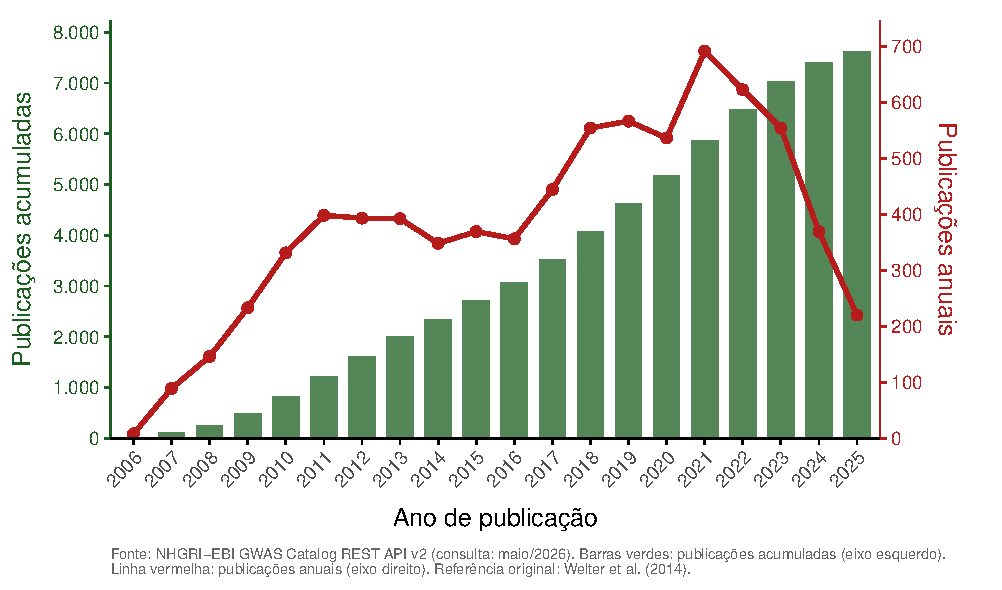
\includegraphics[width=14cm]{figura1_gwas_real.pdf}
  \caption{\novo{Número de publicações sobre GWAS entre 2006 e 2025.}}
  \label{fig:gwas_crescimento}
  \novo{\textit{\textit{National Human Genome Research Institute}--NHGRI\@.
  Adaptado de \citeonline{welter2014}, com atualização baseada em
  \citeonline{Bircan2025}.}}
\end{figure}

\novo{A contagem de publicações foi obtida por meio de consulta programática à
\textit{API REST v2} do \textit{NHGRI-EBI GWAS Catalog}, disponível publicamente
em \url{https://www.ebi.ac.uk/gwas/rest/api/v2/publications}. A busca recuperou
todos os registros de publicações elegíveis cadastrados no catálogo, sem filtros
adicionais de tema, período ou tipo de estudo. A consulta foi realizada em
14 de maio de 2026, retornando um total de 7.690 publicações (campo
\texttt{totalElements} do objeto de paginação da resposta JSON). Os registros
foram recuperados em lotes de 500 entradas por página (\texttt{size=500}), iterando
sobre todas as 16 páginas disponíveis até esgotar o conjunto completo. De cada
registro foi extraído o campo \texttt{publication\_date} (formato
\texttt{YYYY-MM-DD}), do qual se isolou o ano de publicação. As publicações de
2005 ($n = 2$) e de 2026 ($n = 69$, ano incompleto à data da consulta) foram
excluídas da figura, resultando em 7.621 publicações distribuídas entre 2006 e
2025. Os dados brutos estão disponíveis no arquivo
\texttt{gwas\_publicacoes\_por\_ano.csv}, e o código R utilizado para a consulta
e geração da figura encontra-se no arquivo
\texttt{gerar\_figura1\_atualizada.R} e \texttt{buscar\_gwas\_publicacoes.R},
ambos depositados junto ao material suplementar deste trabalho.}



\textbf{Limitações do SMS em sua formulação original.} Os trabalhos que desenvolveram e aplicaram o SMS \cite{de2014snps,Oliveira2015,Souza2022,Baptista2024} operaram exclusivamente ou predominantemente em problemas de regressão (fenótipos contínuos), utilizando Regressão por Vetores Suporte (SVR) e métricas de ajuste como critério de otimalidade. Nenhum desses trabalhos abordou sistematicamente: (i) a adaptação do método para classificação binária com SVM; (ii) o efeito do desbalanceamento de classes sobre a seleção de SNPs; nem (iii) a avaliação simultânea da qualidade da seleção nos dois planos relevantes --- desempenho de classificação dos indivíduos e recuperação dos marcadores causais verdadeiros.

\novo{O único experimento com fenótipo binário presente nessa linha de pesquisa foi a \textbf{Simulação~6} de \citeonline{Oliveira2015}, cujos resultados constituem o ponto de partida direto deste trabalho. Nessa simulação, o SMS foi aplicado a uma base com 8 SNPs causais, 3 com efeitos aditivos isolados (SNPs~1--3, com $\beta_1=2{,}0$, $\beta_2=1{,}3$, $\beta_3=0{,}9$) e 5 participando de interações de ordem~2 e ordem~3, gerando um total de 138 controles e 862 casos --- razão 1:6,25, representativa de uma doença rara. A métrica de aptidão do GA foi a AUC-ROC e \textbf{nenhuma técnica de balanceamento de classes} foi empregada. Os resultados, exibidos na Tabela~\ref{tab:sim6_oliveira} abaixo, revelam dois problemas estruturais:}

\begin{table}[H]
\centering
\caption{\novo{Resultados do SMS na Simulação~6 de \citeonline{Oliveira2015}: SNPs selecionados (total e causais) e AUC média em 10 execuções.}}
\label{tab:sim6_oliveira}
\small
\renewcommand{\arraystretch}{1.3}
\begin{tabular}{L{3.5cm}|C{1.4cm}|C{2.0cm}|C{1.8cm}|C{2.0cm}}
\hline
\textbf{Método / Kernel} & \textbf{Total SNPs} & \textbf{SNPs causais (V)} & \textbf{AUC média} & \textbf{Prec.\ var.\ (\%)} \\
\hline
SMS Linear (União)               & 98 & 6 & 0,595 & 6,1 \\
SMS Radial $\gamma=0{,}001$ (Un.)& 99 & 7 & 0,696 & 7,1 \\
SMS Radial $\gamma=0{,}01$ (Un.) & 68 & 5 & 0,631 & 7,4 \\
SMS Radial $\gamma=0{,}1$ (Un.)  & 93 & 8 & 0,850 & 8,6 \\
SMS Radial $\gamma=1$ (Un.)      & 36 & 8 & 0,833 & \textbf{22,2} \\
Valor-$p$ bruto                  &  7 & 4 & ---   & 57,1 \\
Valor-$p$ corrigido              &  3 & 3 & ---   & 100,0 \\
\hline
\multicolumn{5}{L{10.7cm}}{\footnotesize\textit{Prec.\ var.\ (\%) = SNPs causais / total selecionados $\times$ 100.
  Cálculo retroativo: métrica não reportada em \citeonline{Oliveira2015}.}} \\
\hline
\end{tabular}
\end{table}

\novo{\textbf{Problema~1 --- Alta taxa de falsos positivos.} O melhor resultado do SMS (kernel radial $\gamma=1$, união de 10 execuções) selecionou todos os 8 SNPs causais (Sensibilidade = 100\%), mas ao custo de 28 SNPs não-causais no conjunto final, resultando em Precisão ao nível da variável de apenas 22\%. Para os kernels linear e radiais com $\gamma$ pequeno, a Precisão foi inferior a 10\%, o que tornaria biologicamente inviável qualquer validação experimental subsequente.}

\novo{\textbf{Problema~2 --- Desbalanceamento sem tratamento.} Com 862 casos e apenas 138 controles (87\% vs.\ 13\%), o SVM com critério AUC-ROC foi treinado sobre dados severamente desbalanceados \emph{sem} qualquer correção. \citeonline{Oliveira2015} reconhece explicitamente esse ponto: \textquotedblleft{}nenhuma das técnicas [para o problema de desequilíbrio de classes] foi usada no SMS com intuito de testar o SMS na sua versão mais simples em problemas de classificação com desbalanceamento entre as classes\textquotedblright{} \cite{Oliveira2015}. Essa opção metodológica deixou em aberto a questão de como o balanceamento afeta tanto a classificação dos indivíduos quanto a recuperação dos SNPs causais.}

\novo{Esses dois problemas interligados --- ausência de balanceamento e ausência de avaliação dual ao nível da variável --- configuram a lacuna científica que o presente trabalho se propõe a preencher, adotando SMOTE-NC como mecanismo de balanceamento e introduzindo Precisão, Sensibilidade e F1-Score das variáveis como métricas centrais de avaliação.}

\textbf{Lacuna metodológica na avaliação de seleção de SNPs.} A literatura de \textit{benchmarking} de métodos de seleção de variáveis em dados genômicos \cite{Kollipara2026} tem adotado métricas ao nível da variável (precisão, sensibilidade, F1-Score dos SNPs selecionados) para comparar diferentes abordagens. Contudo, essa estrutura de avaliação dual --- ao nível dos indivíduos \emph{e} ao nível das variáveis --- não havia sido aplicada sistematicamente ao método SMS. Preenchê-la é, ao mesmo tempo, uma necessidade metodológica para o avanço do campo e uma contribuição original deste trabalho.

% =============================================================
\section{Objetivos}

\subsection{\textbf{Objetivo Geral}}

O principal objetivo deste trabalho é modificar o método SMS com a introdução de novos critérios de otimalidade para a seleção de marcadores genéticos relacionados a um certo tipo de fenótipo mapeado por uma variável discreta binária. Este cenário é particularmente desafiador devido à natureza desbalanceada dos dados, em que uma das categorias da variável binária é consideravelmente menos representada. A partir de um conjunto de dados com uma grande quantidade de marcadores genéticos, serão priorizados aqueles que apresentam efeitos marginais significativos e/ou interagem de forma relevante em duplas e trios, com o objetivo de identificar SNPs verdadeiros-positivos e reduzir falsos-positivos.

\subsection{\textbf{Objetivos Específicos}}

Os objetivos específicos são:

$\bullet$ Apresentar o método SMS em sua versão atual com o critério de otimalidade baseado na Acurácia das observações;

$\bullet$ Apresentar uma versão atualizada do SMS baseada em novos critérios de otimalidade, denominados Precisão das Variáveis, Sensibilidade das Variáveis e F1~Score, para lidar de forma mais adequada com bases de dados fenotipicamente desbalanceadas;

$\bullet$ Verificar se o método SMS com o F1~Score apresentará um desempenho superior ao método SMS com a Acurácia na seleção de SNPs causais, em termos de precisão e sensibilidade dos marcadores selecionados;

$\bullet$ Avaliar o desempenho dos critérios de otimalidade usando validação cruzada estratificada e técnicas de balanceamento dos dados por meio do SMOTE-NC (\textit{Synthetic Minority Over-sampling Technique for Nominal and Continuous features}).

% =============================================================
\section{Questões Norteadoras}
\label{sec:questoes}
% =============================================================

A pergunta motivadora apresentada na Seção~1.2 desdobra-se em cinco questões norteadoras, cada uma associada a uma dimensão específica do estudo. As questões foram formuladas a partir das lacunas identificadas na literatura e das decisões metodológicas que distinguem esta adaptação do SMS das versões anteriores.

\bigskip
\noindent As cinco questões norteadoras que operacionalizam a pergunta motivadora são:

\begin{description}
  \item[\textbf{QP1 --- Métrica de otimização:}] O F1-Score como critério de aptidão do Algoritmo Genético produz conjuntos de SNPs mais parcimoniosos e com maior capacidade de recuperação de causais do que a Acurácia em bases de dados fenotipicamente desbalanceadas? Espera-se que sim, pois a Acurácia pode ser maximizada pelo GA explorando o viés da classe majoritária, ao passo que o F1-Score penaliza igualmente falsos positivos e falsos negativos, forçando a busca por marcadores genuinamente discriminativos \cite{he2009learning}.

  \item[\textbf{QP2 --- Protocolo de validação:}] A validação cruzada estratificada preserva melhor a representatividade das classes em cada partição, produzindo estimativas de desempenho mais estáveis e menos viesadas do que a validação cruzada não-estratificada? Espera-se que a estratificação seja especialmente vantajosa em bases desbalanceadas, onde partições aleatórias podem gerar folds com proporções de classe muito distintas do conjunto total \cite{Kohavi1995}.

  \item[\textbf{QP3 --- Balanceamento por reamostragem:}] A aplicação do SMOTE-NC exclusivamente nas partições de treinamento de cada fold restaura a capacidade de recuperação dos SNPs causais em bases desbalanceadas, sem introduzir viés por \textit{data leakage}? Espera-se que o SMOTE-NC aproxime os resultados obtidos com bases desbalanceadas dos resultados das bases balanceadas, ao compensar o sinal da classe minoritária durante o treinamento \cite{chawla2002smote}.

  \item[\textbf{QP4 --- Arquitetura genética e escolha do kernel:}] A estrutura dos efeitos genéticos --- efeitos aditivos independentes versus efeitos epistáticos em grupos --- modifica qual configuração de kernel SVM é mais eficaz na recuperação dos SNPs causais? Espera-se que o kernel Linear seja competitivo com os kernels Radiais em cenários de efeitos aditivos (Base 1), mas que os kernels Radiais sejam superiores em cenários epistáticos (Base 2), dada sua maior capacidade de capturar interações não lineares entre marcadores \cite{vapnik95,scholkopf2002}.

  \item[\textbf{QP5 --- Avaliação dual (observações e variáveis):}] As métricas ao nível das variáveis --- Precisão, Sensibilidade e F1-Score dos SNPs --- revelam aspectos da qualidade da seleção que a Acurácia dos indivíduos não consegue capturar, possibilitando distinguir configurações que acertam as classes por razões espúrias (viés de classe) daquelas que genuinamente identificam os marcadores causais? Espera-se que a avaliação dual evidencie casos em que elevada acurácia individual coexiste com baixa recuperação de causais, demonstrando a necessidade de métricas ao nível das variáveis como critério complementar de avaliação \cite{Kollipara2026}.
\end{description}

\bigskip
\noindent As respostas a essas questões são obtidas por meio de experimentos computacionais controlados com dados simulados, cujos resultados são apresentados e discutidos nos capítulos subsequentes.

\section{Estrutura do Trabalho}

Apresenta-se nesta seção a organização dos capítulos deste trabalho:

$\bullet$ No Capítulo $1$ é apresentada a introdução, compreendendo: o problema de pesquisa (Seção~1.1), a pergunta motivadora (Seção~1.2), a justificativa do estudo (Seção~1.3), os objetivos geral e específicos (Seção~1.4), as questões norteadoras (Seção~1.5) e a estrutura do trabalho (Seção~1.6);

$\bullet$ O Capítulo $2$ apresenta a contextualização dos estudos de associação em escala genômica, descrevendo o crescimento das publicações na área e a motivação para o desenvolvimento de métodos computacionais eficientes para seleção de SNPs;

$\bullet$ O Capítulo $3$ descreve o material e os métodos utilizados, incluindo a geração das bases de dados simuladas, o \textit{pipeline} do método SMS e os parâmetros adotados em cada análise;

$\bullet$ O Capítulo $4$ apresenta as métricas de avaliação dos SNPs --- Precisão das Variáveis, Sensibilidade das Variáveis e F1 das Variáveis --- bem como a Acurácia das Observações, com suas respectivas formulações matemáticas;

$\bullet$ O Capítulo $5$ discute o parâmetro $\gamma$ do SVM-RBF como controle de regularização e sua influência na seleção de SNPs nas etapas de corte e refinamento do SMS;

$\bullet$ O Capítulo $6$ exibe os resultados dos experimentos computacionais para a Base de Dados $1$, com oito efeitos aditivos independentes, para todos os cenários de treinamento e validação investigados;

$\bullet$ O Capítulo $7$ apresenta os resultados referentes à Base de Dados $2$, composta por cinco grupos causais com efeitos epistáticos, para os mesmos cenários experimentais;

$\bullet$ O Capítulo $8$ analisa as diferenças de desempenho do SMS-SVM entre as duas bases simuladas, discutindo o impacto da presença de epistasia na seleção de SNPs;

$\bullet$ O Capítulo $9$ compara as métricas de Acurácia e F1~Score como critérios de otimização do SMS, avaliando seus efeitos sobre a precisão e a sensibilidade das variáveis selecionadas;

$\bullet$ O Capítulo $10$ avalia o efeito do desbalanceamento de classes sobre a seleção de SNPs, analisando a contribuição do SMOTE-NC para a melhoria dos resultados;

$\bullet$ O Capítulo $11$ apresenta a conclusão comparativa, sintetizando as principais descobertas dos dez cenários experimentais e indicando a configuração recomendada do SMS para classificação binária em GWAS;

$\bullet$ Nos Apêndices são apresentados os gráficos gerados nas etapas de corte e refinamento do método SMS-SVM para todos os cenários experimentais avaliados.

% ---- Legenda de cores (nota interna, mantida para referência) ----------------
\begin{center}
\footnotesize
\begin{tabular}{@{}lp{12cm}@{}}
  \textbf{Legenda de Cores:} & \\[2pt]
  \textcolor{black}{\rule{1.2cm}{5pt}} &
    Texto preto: conteúdo original extraído das tabelas de resultados. \\[4pt]
  \textcolor{corNova}{\rule{1.2cm}{5pt}} &
    \novo{Texto azul-petróleo: conteúdo inserido (novos experimentos com
    SMOTE-NC, análises comparativas e conclusões).} \\
\end{tabular}
\end{center}
\vspace{1em}

% =============================================================
\chapter{\textbf{MATERIAL E MÉTODOS}}
% =============================================================

\section*{Geração das Bases de Dados Simuladas}

\novo{As bases de dados foram geradas por meio do modelo linear generalizado para SNPs implementado na função \texttt{simulateSNPglm} do pacote \texttt{scrime} do R \cite{Team2013,Schwender2013,scrime2013}. O modelo gera simultaneamente uma matriz de genótipos e um preditor linear, a partir do qual se define o fenótipo binário (caso/controle). Em ambas as bases, o fenótipo $Y_i$ do indivíduo $i$ é definido pela regra de limiar:}
\begin{equation}
  \novo{Y_i = \mathbf{1}[\eta_i > 0], \qquad
  \eta_i = \beta_0 + \sum_{g=1}^{G} \beta_g \cdot f_g\!\left(\mathbf{x}_i^{(g)}\right) + \varepsilon_i,
  \quad \varepsilon_i \overset{\text{i.i.d.}}{\sim} N(0,1)}
  \label{eq:limiar}
\end{equation}
\novo{onde $\eta_i$ é o preditor linear, $\beta_0$ é o intercepto (calibrado numericamente para atingir a proporção de casos desejada), $G$ é o número de grupos causais, $\beta_g$ é o efeito do grupo $g$, $f_g(\mathbf{x}_i^{(g)})$ é a função de codificação genotípica do grupo $g$ para o indivíduo $i$, e $\varepsilon_i$ é o erro aleatório gaussiano. Para cada SNP $j$ não pertencente a nenhum grupo causal, seu efeito é nulo ($\beta = 0$). O genótipo $x_{ij} \in \{1, 2, 3\}$ é codificado pelo pacote \texttt{scrime} segundo a convenção: $x_{ij} = 1$ indica homozigoto para o alelo maior (AA, zero cópias do alelo menor), $x_{ij} = 2$ indica heterozigoto (Aa, uma cópia) e $x_{ij} = 3$ indica homozigoto para o alelo menor (aa, duas cópias).}

\novo{A função $f_g$ codifica o efeito de cada grupo segundo o modelo genético especificado pelo parâmetro \texttt{list.ia} do \texttt{scrime}. Com a codificação $x \in \{1, 2, 3\}$, os códigos têm os seguintes efeitos sobre o preditor linear:}
\begin{itemize}
  \item \novo{$+1$ (aditivo): $f(x) = x - 1 \in \{0, 1, 2\}$ --- efeito proporcional ao número de cópias do alelo menor.}
  \item \novo{$+2$ (dominante): $f(x) = \mathbf{1}[x \geq 2] \in \{0, 1\}$ --- efeito presente sempre que ao menos uma cópia do alelo menor existe (Aa ou aa).}
  \item \novo{$+3$ (recessivo): $f(x) = \mathbf{1}[x = 3] \in \{0, 1\}$ --- efeito presente apenas no homozigoto menor (aa).}
  \item \novo{$-1$ (reverso aditivo): $f(x) = 3 - x \in \{0, 1, 2\}$ --- efeito decrescente com o número de cópias do alelo menor.}
  \item \novo{$-2$ (reverso dominante): $f(x) = \mathbf{1}[x = 1] \in \{0, 1\}$ --- efeito presente apenas no homozigoto maior (AA).}
  \item \novo{$-3$ (reverso recessivo): $f(x) = \mathbf{1}[x \leq 2] \in \{0, 1\}$ --- efeito presente quando não há homozigotia para o alelo menor.}
\end{itemize}
\novo{A Tabela~\ref{tab:fx_exemplos} ilustra os valores de $f(x)$ para cada modelo genético, dado o genótipo observado do indivíduo:}

\begin{table}[H]
\centering
\caption{\novo{Valores de $f(x)$ por modelo genético e genótipo (codificação \texttt{scrime}: $x=1$ = AA, $x=2$ = Aa, $x=3$ = aa).}}
\label{tab:fx_exemplos}
\small
\renewcommand{\arraystretch}{1.35}
\begin{tabular}{llccc}
\hline
\textbf{Código} & \textbf{Modelo} & \textbf{$f(1)$ (AA)} & \textbf{$f(2)$ (Aa)} & \textbf{$f(3)$ (aa)} \\
\hline
$+1$ & Aditivo             & $0$ & $1$ & $2$ \\
$+2$ & Dominante           & $0$ & $1$ & $1$ \\
$+3$ & Recessivo           & $0$ & $0$ & $1$ \\
$-1$ & Reverso aditivo     & $2$ & $1$ & $0$ \\
$-2$ & Reverso dominante   & $1$ & $0$ & $0$ \\
$-3$ & Reverso recessivo   & $1$ & $1$ & $0$ \\
\hline
\end{tabular}
\end{table}

\novo{\textbf{Fundamento biológico e interpretação de cada modelo.} Os seis modelos codificam os principais mecanismos de ação alélica conhecidos em genética quantitativa. A seguir cada modelo é explicado com sua lógica biológica.}

\begin{description}

  \item[\novo{$\boldsymbol{+1}$ --- Aditivo $[f = 0,\;1,\;2]$:}]
  \novo{Cada cópia do alelo 'a' adiciona uma unidade igual de efeito ao preditor. O heterozigoto Aa contribui exatamente com a metade do homozigoto aa --- o que se denomina ausência de dominância. Matematicamente, $f(x) = x - 1$, que é equivalente a contar o número de alelos 'a' ($0$, $1$ ou $2$). Este é o modelo padrão em GWAS, utilizado na regressão linear de fenótipo em contagem alélica, pois é o mais simples e mais poderoso quando a relação genótipo--fenótipo é realmente linear. Em termos moleculares, representa situações em que cada cópia do gene funcional produz uma dose proporcional de proteína (haploinsuficiência quantitativa).}

  \item[\novo{$\boldsymbol{+2}$ --- Dominante $[f = 0,\;1,\;1]$:}]
  \novo{O alelo 'a' é dominante: basta \textbf{uma} cópia para produzir o efeito pleno. O heterozigoto Aa é fenotipicamente idêntico ao homozigoto aa --- a presença de 'a' "suprime" o alelo 'A'. Matematicamente, $f(x) = \mathbf{1}[x \geq 2]$. Por que Aa e aa recebem o mesmo valor $f = 1$? Porque no modelo dominante, a segunda cópia de 'a' não agrega efeito adicional --- o sistema já saturou na primeira. Biologicamente, ocorre quando o produto do alelo 'a' (por exemplo, uma proteína com ganho-de-função) é suficiente em dose simples para alterar o fenótipo. Um exemplo clássico são mutações causadoras de doenças autossômicas dominantes: portadores Aa são afetados assim como os homozigotos aa.}

  \item[\novo{$\boldsymbol{+3}$ --- Recessivo $[f = 0,\;0,\;1]$:}]
  \novo{O alelo 'a' é recessivo: o efeito \textbf{só se manifesta com duas cópias} (homozigoto aa). Em heterozigose Aa, o alelo 'A' é dominante e mascara completamente a ação de 'a'. Matematicamente, $f(x) = \mathbf{1}[x = 3]$. Por que Aa recebe $f = 0$? Porque a única cópia de 'a' presente é "silenciada" pelo alelo A dominante. Biologicamente, representa perda-de-função (loss-of-function): um único alelo funcional residual ('A') produz proteína suficiente para manter o fenótipo normal; somente a ausência completa de alelos funcionais (aa) causa o efeito. Doenças recessivas clássicas como fibrose cística e anemia falciforme seguem este modelo.}

  \item[\novo{$\boldsymbol{-1}$ --- Reverso aditivo $[f = 2,\;1,\;0]$:}]
  \novo{O espelho exato do modelo aditivo: agora é o alelo \textbf{A} (majoritário) que carrega o risco, e cada cópia adicional de 'a' \textit{reduz} o efeito. Matematicamente, $f_{-1}(x) = 2 - f_{+1}(x) = 3 - x$, que equivale a contar o número de alelos 'A'. Biologicamente, representa cenários em que o alelo ancestral comum 'A' é o alelo de risco e o alelo derivado 'a' é protetor. Estudos de GWAS descobriram variantes desse tipo em certas populações: o alelo mais frequente é o deletério porque confere vantagem em outros contextos evolutivos.}

  \item[\novo{$\boldsymbol{-2}$ --- Reverso dominante $[f = 1,\;0,\;0]$:}]
  \novo{O complemento do modelo dominante ($f_{-2}(x) = 1 - f_{+2}(x)$): somente o homozigoto AA expressa o efeito. Qualquer presença de 'a' --- mesmo em dose simples --- suprime o efeito de A. Matematicamente, $f(x) = \mathbf{1}[x = 1]$. A interpretação é que 'a' age como \textbf{dominante supressor}: um único alelo 'a' em heterozigose já é suficiente para anular a ação de 'A'. Para o efeito de A se manifestar, é preciso que não haja nenhuma cópia de 'a' --- ou seja, o indivíduo precisa ser homozigoto AA. Do ponto de vista de 'A', isso equivale a um comportamento \textbf{recessivo} (duas cópias de A são necessárias para expressar o efeito). O modelo é o mais difícil de detectar em GWAS porque apenas o grupo AA (proporcional a $(1-q)^2$, onde $q$ é a frequência de 'a') tem efeito diferente dos demais.}

  \item[\novo{$\boldsymbol{-3}$ --- Reverso recessivo $[f = 1,\;1,\;0]$:}]
  \novo{O complemento do modelo recessivo ($f_{-3}(x) = 1 - f_{+3}(x)$): AA e Aa são ambos afetados; somente o homozigoto aa perde o efeito. Matematicamente, $f(x) = \mathbf{1}[x \leq 2]$. O alelo 'a' age como \textbf{recessivo supressor}: são necessárias \textit{duas cópias} de 'a' para eliminar o efeito de A. Uma única cópia de 'a' em Aa é insuficiente --- A ainda consegue manter o efeito. Do ponto de vista de A, isso é um comportamento \textbf{dominante}: basta um alelo A para manter o fenótipo. A diferença em relação a +2 está apenas em qual alelo é o ativo: em +2, 'a' ativa o efeito com uma cópia; em -3, 'A' mantém o efeito com uma cópia.}

\end{description}

\novo{\textbf{Padrão de complementaridade entre modelos positivos e negativos.} Uma propriedade estrutural importante é que os três modelos negativos são exatamente o complemento aritmético dos positivos:}
\begin{align*}
  f_{-1}(x) &= 2 - f_{+1}(x) \quad \Rightarrow \quad [2,\,1,\,0] = 2 - [0,\,1,\,2] \\
  f_{-2}(x) &= 1 - f_{+2}(x) \quad \Rightarrow \quad [1,\,0,\,0] = 1 - [0,\,1,\,1] \\
  f_{-3}(x) &= 1 - f_{+3}(x) \quad \Rightarrow \quad [1,\,1,\,0] = 1 - [0,\,0,\,1]
\end{align*}
\novo{Em todos os casos, o modelo negativo inverte o papel dos alelos: onde o modelo positivo colocava 'a' como alelo de risco, o negativo coloca 'A'. Os seis modelos cobrem, portanto, \textbf{todo o espectro de arquiteturas genéticas monogênicas} --- aditiva, dominante e recessiva --- para ambos os sentidos de efeito alélico. Na simulação, cada SNP causal recebe um código de modelo independente, criando um cenário heterogêneo que testa a capacidade do SMS de recuperar marcadores sem assumir nenhuma arquitetura específica.}

\novo{\textbf{Exemplo numérico.} Considere um indivíduo hipotético com dois SNPs causais: SNP\,1 com genótipo Aa ($x=2$, modelo aditivo, $\beta_1 = 2$) e SNP\,2 com genótipo aa ($x=3$, modelo dominante, $\beta_2 = 2$). Suponha $\beta_0 = -1$ e $\varepsilon_i = 0{,}3$:
\begin{align*}
f_1(2) &= 2 - 1 = 1 \quad \text{(aditivo)}, \\
f_2(3) &= \mathbf{1}[3 \geq 2] = 1 \quad \text{(dominante)}, \\
\eta_i  &= -1 + 2\cdot 1 + 2\cdot 1 + 0{,}3 = 3{,}3 > 0 \implies Y_i = 1 \text{ (caso)}.
\end{align*}
Se o mesmo indivíduo tivesse SNP\,2 com genótipo AA ($x=1$, dominante): $f_2(1) = \mathbf{1}[1 \geq 2] = 0$, e então $\eta_i = -1 + 2\cdot 1 + 2\cdot 0 + 0{,}3 = 1{,}3 > 0$, ainda classificado como caso. Mas se SNP\,1 fosse AA ($x=1$, aditivo): $f_1(1) = 0$, resultando em $\eta_i = -1 + 0 + 0 + 0{,}3 = -0{,}7 \leq 0 \implies Y_i = 0$ (controle). Esses exemplos mostram como a ausência do alelo menor em ambos os SNPs causais pode inverter a classificação do fenótipo.}

\novo{Para grupos com múltiplos SNPs, a função $f_g$ é o produto das codificações individuais de cada SNP do grupo, modelando interações epistáticas entre os marcadores.}

\novo{A frequência do alelo menor (MAF) de cada SNP foi sorteada uniformemente no intervalo $[0{,}1;\; 0{,}4]$. Os SNPs não causais foram gerados sem qualquer associação com o fenótipo.}

\subsection*{Calibração de $\beta_0$ para Controle do Balanceamento de Classes}

\novo{O intercepto $\beta_0$ atua como um deslocamento (\textit{shift}) global do preditor linear $\eta_i$: valores mais negativos de $\beta_0$ empurram os preditores para abaixo de zero, reduzindo a proporção de casos ($Y_i = 1$), enquanto valores mais positivos a aumentam. Portanto, para controlar a razão casos/controles, é necessário encontrar o $\beta_0^*$ tal que a proporção esperada de casos seja exatamente o valor-alvo $p^* \in (0,1)$.}

\novo{O processo de calibração, implementado na função \texttt{find\_beta0\_for\_target} do código em R, segue os seguintes passos:
\begin{enumerate}
  \item Definir a função-objetivo $h(\beta_0) = \widehat{p}(\beta_0) - p^*$, em que $\widehat{p}(\beta_0)$ é a proporção amostral de casos obtida ao simular os dados com aquele intercepto (média de 3 réplicas para reduzir ruído estocástico).
  \item Verificar se o intervalo inicial $[\beta_0^L, \beta_0^U] = [-20,\, 20]$ é um \textit{bracket} válido, ou seja, se $h(\beta_0^L)$ e $h(\beta_0^U)$ têm sinais opostos. Caso contrário, o intervalo é expandido em $\pm 10$ unidades, até no máximo 5 vezes.
  \item Aplicar o método da bisseção (\texttt{uniroot} do R) nesse intervalo, com tolerância $\delta = 10^{-3}$, até encontrar $\beta_0^*$ tal que $|h(\beta_0^*)| < \delta$.
  \item Simular a base final com esse $\beta_0^*$ e, se necessário, forçar exatamente $n_1$ casos pelo ranqueamento decrescente de $\eta_i$ (opção \texttt{exact\_by\_rank}).
\end{enumerate}}

\novo{\textbf{Exemplo numérico --- Base Balanceada (500 casos / 500 controles).} Seja $p^* = 0{,}50$ com $n = 1000$ observações. A função-objetivo vale:
\begin{align*}
h(\beta_0) &= \widehat{p}(\beta_0) - 0{,}50.
\end{align*}
A Tabela~\ref{tab:bissecao_bal} ilustra as iterações da bisseção até a convergência:}

\begin{table}[H]
\centering
\caption{\novo{Iterações da bisseção para $p^* = 0{,}50$ (base balanceada). Valores de $\widehat{p}$ são proporções estimadas por simulação.}}
\label{tab:bissecao_bal}
\small
\renewcommand{\arraystretch}{1.3}
\begin{tabular}{cccccc}
\hline
\textbf{Iter.} & $\beta_0^L$ & $\beta_0^U$ & $\beta_0^{\text{meio}}$ & $\widehat{p}(\beta_0^{\text{meio}})$ & $h(\beta_0^{\text{meio}})$ \\
\hline
1 & $-20{,}0$ & $20{,}0$ & $ 0{,}00$ & $0{,}82$ & $+0{,}32$ \\
2 & $-20{,}0$ & $ 0{,}0$ & $-10{,}00$ & $0{,}03$ & $-0{,}47$ \\
3 & $-10{,}0$ & $ 0{,}0$ & $ -5{,}00$ & $0{,}51$ & $+0{,}01$ \\
4 & $-10{,}0$ & $-5{,}0$ & $ -7{,}50$ & $0{,}19$ & $-0{,}31$ \\
5 & $ -7{,}5$ & $-5{,}0$ & $ -6{,}25$ & $0{,}34$ & $-0{,}16$ \\
\multicolumn{3}{c}{$\cdots$} & $\approx -5{,}06$ & $0{,}500$ & $\approx 0$ \\
\hline
\end{tabular}
\end{table}

\novo{O valor convergido $\beta_0^* \approx -5{,}06$ é então usado na simulação final. Como os coeficientes $\beta_g = 2$ elevam sistematicamente $\eta_i$ (os efeitos genéticos contribuem positivamente para os casos), é necessário um intercepto negativo para compensar e manter a proporção em 50\%.}

\novo{\textbf{Exemplo numérico --- Base Desbalanceada (200 casos / 800 controles).} Para $p^* = 0{,}20$, a proporção-alvo é mais baixa, exigindo um intercepto ainda mais negativo. A Tabela~\ref{tab:bissecao_desbal} mostra as primeiras iterações:}

\begin{table}[H]
\centering
\caption{\novo{Iterações da bisseção para $p^* = 0{,}20$ (base desbalanceada). Valores de $\widehat{p}$ são proporções estimadas por simulação.}}
\label{tab:bissecao_desbal}
\small
\renewcommand{\arraystretch}{1.3}
\begin{tabular}{cccccc}
\hline
\textbf{Iter.} & $\beta_0^L$ & $\beta_0^U$ & $\beta_0^{\text{meio}}$ & $\widehat{p}(\beta_0^{\text{meio}})$ & $h(\beta_0^{\text{meio}})$ \\
\hline
1 & $-20{,}0$ & $20{,}0$ & $ 0{,}00$ & $0{,}82$ & $+0{,}62$ \\
2 & $-20{,}0$ & $ 0{,}0$ & $-10{,}00$ & $0{,}03$ & $-0{,}17$ \\
3 & $-10{,}0$ & $ 0{,}0$ & $ -5{,}00$ & $0{,}51$ & $+0{,}31$ \\
4 & $-10{,}0$ & $-5{,}0$ & $ -7{,}50$ & $0{,}19$ & $-0{,}01$ \\
5 & $ -7{,}5$ & $-5{,}0$ & $ -6{,}25$ & $0{,}34$ & $+0{,}14$ \\
\multicolumn{3}{c}{$\cdots$} & $\approx -7{,}43$ & $0{,}200$ & $\approx 0$ \\
\hline
\end{tabular}
\end{table}

\novo{O valor convergido $\beta_0^* \approx -7{,}43$ reflete a necessidade de deslocar mais negativamente o preditor para restringir a proporção de casos a 20\%. A Tabela~\ref{tab:beta0_resumo} resume os interceptos encontrados para cada cenário:}

\begin{table}[H]
\centering
\caption{\novo{Interceptos $\beta_0^*$ calibrados por cenário de simulação.}}
\label{tab:beta0_resumo}
\small
\renewcommand{\arraystretch}{1.3}
\begin{tabular}{lcccc}
\hline
\textbf{Cenário} & \textbf{Casos ($n_1$)} & \textbf{Controles ($n_0$)} & $p^*$ & $\beta_0^*$ (aprox.) \\
\hline
Base Balanceada    & 500 & 500 & 0{,}50 & $-5{,}06$ \\
Base Desbalanceada & 200 & 800 & 0{,}20 & $-7{,}43$ \\
\hline
\end{tabular}
\end{table}

\subsection*{Base de Dados 1 --- Oito Efeitos Independentes}

\novo{A Base 1 foi simulada com $G = 8$ grupos causais, cada um contendo exatamente um SNP causal (efeitos marginais independentes, sem interação entre eles). O preditor linear é:}
\begin{multline}
  \color{corNova}
  \eta_i = \beta_0 + 2\,g_1(x_{i1}) + 2\,g_2(x_{i2}) + 2\,g_3(x_{i3}) + 2\,g_{-1}(x_{i4}) \\
         + 2\,g_{-2}(x_{i5}) + 2\,g_{-3}(x_{i6}) + 2\,g_1(x_{i7}) + 2\,g_2(x_{i8}) + \varepsilon_i
  \label{eq:base1}
\end{multline}
\novo{onde os subíndices de $g$ indicam o modelo genético: $g_1$ (aditivo), $g_2$ (dominante), $g_3$ (recessivo), $g_{-1}$ (reverso aditivo), $g_{-2}$ (reverso dominante), $g_{-3}$ (reverso recessivo). Todos os coeficientes $\beta_g = 2$. Os SNPs causais são SNP\,1 a SNP\,8; os demais 92 SNPs não têm efeito sobre o fenótipo.}

\subsection*{Base de Dados 2 --- Cinco Grupos com Efeitos Epistáticos}

\novo{A Base 2 foi simulada com $G = 5$ grupos causais, contendo ao todo 8 SNPs causais agrupados por padrão de interação epistática. O preditor linear é:}
\begin{equation}
  \novo{\eta_i = \beta_0
         + 2\,g_1(x_{i1})
         + 2\,g_3(x_{i2})
         + 2\,g_2(x_{i3})
         + 3\,g_{-1,3}(x_{i4}, x_{i5})
         + 4\,g_{1,2,3}(x_{i6}, x_{i7}, x_{i8})
         + \varepsilon_i}
  \label{eq:base2}
\end{equation}
\novo{onde $g_{-1,3}(x_{i4}, x_{i5}) = g_{-1}(x_{i4}) \cdot g_3(x_{i5})$ representa a interação epistática entre SNP\,4 (reverso aditivo) e SNP\,5 (recessivo), e $g_{1,2,3}(x_{i6}, x_{i7}, x_{i8}) = g_1(x_{i6}) \cdot g_2(x_{i7}) \cdot g_3(x_{i8})$ representa a interação epistática tripla entre SNP\,6 (aditivo), SNP\,7 (dominante) e SNP\,8 (recessivo). Os coeficientes $\beta_g$ são 2, 2, 2, 3 e 4 para os grupos 1 a 5, respectivamente, refletindo efeitos crescentes para os grupos epistáticos.}

\section*{Pipeline do Método SMS}

\novo{O método SMS (\textit{SNP Markers Selector}) \cite{de2014snps,Oliveira2015,Souza2022,Baptista2024} é executado em três etapas sequenciais para cada kernel SVM:}
\begin{enumerate}
  \item \novo{\textbf{Ranking por Floresta Aleatória (RF) \cite{breiman2001random,RF,goldstein2011random}:} treina-se uma RF com \texttt{ntree} = 4000 árvores sobre o \textbf{conjunto completo de SNPs da base original} --- sem qualquer balanceamento sintético --- e ordena-se os marcadores pela importância média \textit{Mean Decrease in Gini} (gVI), do mais ao menos relevante. \textbf{Importante:} o SMOTE-NC \emph{não} é aplicado nesta etapa; ele atua exclusivamente dentro das partições de treinamento das etapas~2 e~3, evitando que amostras sintéticas interfiram no ranqueamento global. A escolha do gVI segue \citeonline{Oliveira2015}, que comparou empiricamente o gVI com o índice de importância por permutação (\textit{Permutation Variable Importance}, pVI) e verificou resultados superiores do gVI para o ranqueamento de SNPs nesse contexto, embora sem reportar os valores detalhados. Uma discussão teórica e empírica sobre as propriedades e o comportamento esperado de ambos os índices --- em problemas de regressão e de classificação --- é apresentada no Capítulo~\ref{cap:gvi_pvi}.}
  \item \novo{\textbf{Etapa de Corte do SVM (\textit{Cutting Step}) \cite{vapnik95,chang2011libsvm,e1071}:} o SVM é treinado e avaliado iterativamente: a cada iteração, o SNP de menor rank é removido e o desempenho (acurácia ou F1 Score, conforme o experimento) é registrado. O subconjunto de SNPs que maximiza essa métrica é retido para a próxima etapa.}
  \item \novo{\textbf{Refinamento por Algoritmo Genético (GA) \cite{Goldberg1989,scrucca2012ga}:} sobre o subconjunto retido, o GA busca o subconjunto ótimo de SNPs que maximiza o fitness do SVM (acurácia ou F1 Score). A aptidão é avaliada por $k$-fold com $k=10$ (estratificado ou não-estratificado, conforme o experimento) \cite{Kohavi1995}. O resultado final de cada kernel é o subconjunto identificado pelo GA.}
\end{enumerate}

\begin{figure}[H]
\centering
\resizebox{0.96\textwidth}{!}{%
\begin{tikzpicture}[
  >=Latex,
  procbox/.style={rectangle,rounded corners=4pt,draw=black!50,thick,fill=white,
    text width=4.2cm,minimum height=1.2cm,align=center,font=\small},
  decbox/.style={diamond,draw=black!50,thick,fill=white,aspect=3.5,align=center,
    inner sep=2pt,font=\small},
  stagebox/.style={rectangle,dashed,thick,rounded corners=6pt,
    inner xsep=10pt,inner ysep=10pt},
  stagelbl/.style={font=\small\bfseries,rotate=90,anchor=center},
  notebox/.style={text width=4.4cm,align=left,font=\scriptsize},
  arrow/.style={-{Latex[length=2.5mm,width=1.5mm]},thick},
  % estilos por etapa
  cord/.style={draw=blue!60!black,  fill=blue!8},
  ccor/.style={draw=teal!60!black,  fill=teal!8},
  cref/.style={draw=orange!60!black,fill=orange!8},
  nORD/.style={procbox,draw=blue!60!black,   fill=blue!12},
  nCOR/.style={procbox,draw=teal!60!black,   fill=teal!12},
  nREF/.style={procbox,draw=orange!60!black, fill=orange!12},
  nDEC/.style={decbox, draw=orange!60!black, fill=orange!12},
  nFIN/.style={procbox,draw=violet!60!black, fill=violet!10}
]
% ── Coluna de x fixo para anotações e rótulos ────────────────────────────────
% (definidas após os nós para usar suas coordenadas)

% ── Nós do fluxo ─────────────────────────────────────────────────────────────
% entrada (cinza neutro)
\node[procbox,text width=3.0cm,draw=gray!60,fill=gray!8]
  (dados){\iconDB[0.55]\\[4pt]Dados após CQ};
% ORDENAÇÃO – azul
\node[nORD,below=0.9cm of dados]
  (N1){\iconArvore[0.50]\quad Ordenação dos SNPs\\por cromossomo};
% CORTE – verde-água
\node[nCOR,below=0.9cm of N1]
  (N2){\iconFunil[0.50]\quad Seleção conjunta dos\\SNPs mais informativos\\por cromossomo};
\node[nCOR,below=0.7cm of N2]
  (N3){\iconMonitor[0.50]\quad Junção dos SNPs\\selecionados};
% REFINAMENTO – laranja
\node[nREF,below=0.9cm of N3]
  (N4){\iconLupa[0.50]\quad Busca pelo melhor\\subconjunto de SNPs};
\node[nDEC,below=0.9cm of N4]
  (N5){Atingiu as $i$ execuções?};
% RESULTADO – violeta
\node[nFIN,below=0.9cm of N5]
  (N6){\iconVenn[0.44]\;\iconIntersec[0.44]\\[4pt]União e Interseção\\dos $i$ subconjuntos\\de SNPs};

% ── Setas ────────────────────────────────────────────────────────────────────
\draw[arrow](dados)--(N1);
\draw[arrow](N1)--(N2);
\draw[arrow](N2)--(N3);
\draw[arrow](N3)--(N4);
\draw[arrow](N4)--(N5);
\draw[arrow](N5)--node[right,font=\scriptsize,xshift=2pt]{Sim}(N6);
\draw[arrow](N5.west)--++(-2.6,0)|-node[above,font=\scriptsize,xshift=-8pt]{Não}(N4.west);

% ── Caixas tracejadas ─────────────────────────────────────────────────────────
\begin{scope}[on background layer]
  \node[stagebox,cord,fit=(N1)](stageORD){};
  \node[stagebox,ccor,fit=(N2)(N3)](stageCOR){};
  \node[stagebox,cref,fit=(N4)(N5)](stageREF){};
\end{scope}

% ── Rótulos das etapas (coluna fixa à esquerda, centrados no bloco) ──────────
% LBLX: x da coluna dos rótulos; usa |- para projetar o y de cada stagebox
\coordinate(LBLX) at ($(stageORD.west)+(-1.0cm,0)$);
\node[stagelbl,blue!70!black]   at (LBLX |- stageORD.center) {ORDENAÇÃO};
\node[stagelbl,teal!70!black]   at (LBLX |- stageCOR.center) {CORTE};
\node[stagelbl,orange!70!black] at (LBLX |- stageREF.center) {REFINAMENTO};

% ── Anotações à direita (coluna fixa, sem sobrepor o fluxograma) ─────────────
% ANNX: posicionado 3 cm além da borda direita das caixas do fluxo
\coordinate(ANNX) at ($(N1.east)+(3.0cm,0)$);
\node[notebox,anchor=west] at (ANNX |- dados.center)
  {Arquivo inicial com genótipo e fenótipo após CQ.};
\node[notebox,anchor=west] at (ANNX |- stageORD.center)
  {$\bullet$~RF.\\[2pt]
   $\bullet$~Pacote \texttt{randomForest} do~R.\\[2pt]
   $\bullet$~$\sim$5\% do tempo total.};
\node[notebox,anchor=west] at (ANNX |- stageCOR.center)
  {$\bullet$~SVR ou SVM sobre o \textit{rank} da RF.\\[2pt]
   $\bullet$~Pacote \texttt{e1071} do~R.\\[2pt]
   $\bullet$~$\sim$15\% do tempo total.};
\node[notebox,anchor=west] at (ANNX |- stageREF.center)
  {$\bullet$~GA com SVR ou SVM.\\[2pt]
   $\bullet$~Pacote \texttt{GA} do~R.\\[2pt]
   $\bullet$~$\sim$80\% do tempo total.};
\node[notebox,anchor=west] at (ANNX |- N6.center)
  {Solução final do SMS (união e interseção dos subconjuntos de cada kernel).};
\end{tikzpicture}%
}
\caption{\novo{Fluxograma das etapas do método SMS tanto para regressão quanto para classificação binária.}}
\label{fig:fluxograma_sms}
\novo{Adaptado de \citeonline{Oliveira2015}.}
\end{figure}

\novo{Os resultados de todos os kernels são então combinados por três métodos: \textbf{União} (SNPs selecionados por ao menos um kernel), \textbf{Interseção} (SNPs selecionados por todos os kernels) e \textbf{Valor-$p$} (regressão logística univariada para cada SNP, sem e com correção por múltiplos testes por Bonferroni).}

\section*{Parâmetros e Configurações das Análises}

\novo{A Tabela~\ref{tab:params} resume todos os parâmetros e configurações utilizados nos dez experimentos realizados.}

\begin{table}[H]
\centering
\caption{\novo{Parâmetros e configurações de todas as análises realizadas.}}
\label{tab:params}
\footnotesize
\setlength{\tabcolsep}{3pt}
\renewcommand{\arraystretch}{1.4}
\begin{tabular}{L{3.8cm}|C{1.0cm}|C{1.0cm}|C{1.1cm}|C{1.6cm}|C{1.5cm}|C{1.4cm}|C{1.4cm}}
\hline
\textbf{Experimento} & \textbf{Base} & \textbf{Casos} & \textbf{Contr.} & \textbf{Validação} & \textbf{Balanc.} & \textbf{Métrica Corte} & \textbf{Fitness GA} \\
\hline
Bal.\ $\times$ Val.\ Bal. & 1 & 500 & 500 & $k$-fold estrat.\ $k=10$ & --- & Acurácia & Acurácia \\
\hline
Bal.\ $\times$ Val.\ Desbal. & 1 & 500 & 500 & $k$-fold $k=10$ & --- & Acurácia & Acurácia \\
\hline
Desbal.\ $\times$ Val.\ Bal. & 1 & 200 & 800 & $k$-fold estrat.\ $k=10$ & --- & Acurácia & Acurácia \\
\hline
Desbal.\ $\times$ Val.\ Desbal. & 1 & 200 & 800 & $k$-fold $k=10$ & --- & Acurácia & Acurácia \\
\hline
Desbal.\ + SMOTE (Ac.) & 1 & 200 & 800 & $k$-fold estrat.\ $k=10$ & SMOTE-NC & Acurácia & Acurácia \\
\hline
Desbal.\ + SMOTE (F1) & 1 & 200 & 800 & $k$-fold estrat.\ $k=10$ & SMOTE-NC & F1 Score & F1 Score \\
\hline
Bal.\ $\times$ Val.\ Bal. & 2 & 500 & 500 & $k$-fold estrat.\ $k=10$ & --- & Acurácia & Acurácia \\
\hline
Bal.\ $\times$ Val.\ Desbal. & 2 & 500 & 500 & $k$-fold $k=10$ & --- & Acurácia & Acurácia \\
\hline
Desbal.\ + SMOTE (Ac.) & 2 & 200 & 800 & $k$-fold estrat.\ $k=10$ & SMOTE-NC & Acurácia & Acurácia \\
\hline
Desbal.\ + SMOTE (F1) & 2 & 200 & 800 & $k$-fold estrat.\ $k=10$ & SMOTE-NC & F1 Score & F1 Score \\
\hline
\multicolumn{8}{l}{\textit{Parâmetros comuns a todos os experimentos:}} \\
\multicolumn{8}{l}{SNPs totais = 100 \quad SNPs causais = 8 \quad MAF $\sim U[0{,}1;\,0{,}4]$ \quad RF: ntree = 4000} \\
\multicolumn{8}{l}{SVM: $C = 1{,}0$ \quad Kernels: Linear; RBF $\gamma \in \{0{,}001;\,0{,}01;\,0{,}1;\,1{,}0\}$} \\
\multicolumn{8}{l}{GA: popSize = 100 \quad maxiter = 10 \quad $p_{\text{cross}} = 0{,}8$ \quad $p_{\text{mut}} = 0{,}1$} \\
\hline
\end{tabular}
\end{table}
\renewcommand{\arraystretch}{1.3}

% =============================================================
\section*{SMOTE-NC: Técnica de Balanceamento de Classes por Sobre-amostragem Sintética}
\label{sec:smote}
% =============================================================

\subsection*{Motivação e Problema do Desbalanceamento}

\novo{Em estudos GWAS com fenótipos binários, a proporção entre casos (indivíduos afetados) e controles (indivíduos não afetados) raramente é equilibrada. Doenças raras ou de baixa prevalência produzem bases com razões de 1:4, 1:9 ou até mais extremas. Esse desequilíbrio representa um desafio fundamental para algoritmos de aprendizado de máquina como o SVM: ao minimizar o erro global de classificação, o algoritmo tende a favorecer a classe majoritária, pois acertar todos os controles já garante alta acurácia. Indivíduos da classe minoritária (casos) são frequentemente classificados incorretamente, e os SNPs que distinguem essas classes ficam subrepresentados no processo de seleção \cite{krawczyk2016,he2009learning}.}

\novo{O impacto direto sobre a seleção de SNPs é que o Algoritmo Genético, ao maximizar a acurácia do SVM sobre dados desbalanceados, aprende a explorar o viés da classe majoritária em vez de identificar os marcadores causais verdadeiros. SNPs com efeito real sobre a classe minoritária podem ser ignorados ou descartados nas etapas de corte e refinamento do SMS, pois sua presença contribui pouco para a acurácia total do classificador.}

\subsection*{SMOTE Original: fundamento algorítmico}

\novo{O SMOTE (\textit{Synthetic Minority Over-sampling Technique}), proposto por \citeonline{chawla2002smote}, é a técnica de balanceamento por sobre-amostragem sintética mais utilizada na literatura \cite{fernandez2018smote}. Sua ideia central é gerar \textbf{novas amostras sintéticas} da classe minoritária --- não cópias idênticas de amostras existentes (sobre-amostragem simples por reposição), mas \textbf{interpolações} entre amostras reais da classe minoritária.}

\novo{O algoritmo SMOTE para variáveis contínuas funciona da seguinte forma:}
\begin{enumerate}
  \item \novo{Para cada amostra da classe minoritária $\mathbf{x}_i$, identifica seus $k$ vizinhos mais próximos na mesma classe (usualmente $k = 5$).}
  \item \novo{Seleciona aleatoriamente um vizinho $\mathbf{x}_{nn}$ dentre os $k$ identificados.}
  \item \novo{Gera uma nova amostra sintética por interpolação linear:
  \begin{equation}
    \mathbf{x}_{\text{sint}} = \mathbf{x}_i + \lambda \cdot (\mathbf{x}_{nn} - \mathbf{x}_i), \quad \lambda \sim U[0, 1]
    \label{eq:smote}
  \end{equation}
  onde $\lambda$ é um número aleatório uniforme entre 0 e 1. A nova amostra é posicionada aleatoriamente no segmento de reta que une $\mathbf{x}_i$ ao vizinho $\mathbf{x}_{nn}$.}
  \item \novo{Repete o processo até que a classe minoritária atinja a proporção desejada (tipicamente 50\%/50\%).}
\end{enumerate}

\novo{\textbf{Exemplo numérico (SMOTE contínuo).} Suponha duas amostras da classe minoritária com dois atributos contínuos: $\mathbf{x}_1 = (2{,}0,\; 5{,}0)$ e $\mathbf{x}_2 = (4{,}0,\; 3{,}0)$. Com $\lambda = 0{,}6$:
\begin{align*}
  \mathbf{x}_{\text{sint}} &= (2{,}0,\; 5{,}0) + 0{,}6 \cdot \big[(4{,}0,\; 3{,}0) - (2{,}0,\; 5{,}0)\big] \\
                           &= (2{,}0,\; 5{,}0) + 0{,}6 \cdot (2{,}0,\; -2{,}0) \\
                           &= (2{,}0 + 1{,}2,\; 5{,}0 - 1{,}2) = (3{,}2,\; 3{,}8).
\end{align*}
A nova amostra $(3{,}2;\; 3{,}8)$ não existia nos dados originais --- ela foi criada sinteticamente no espaço de características, no interior da região ocupada pelas amostras da classe minoritária.}

\subsection*{SMOTE-NC: extensão para atributos mistos (nominais e contínuos)}

\novo{Dados genômicos contêm SNPs codificados como variáveis nominais ou ordinais discretas ($x \in \{1, 2, 3\}$ representando AA, Aa, aa), não contínuas. A interpolação direta da Equação~(\ref{eq:smote}) não é adequada para essas variáveis, pois um valor interpolado como $1 + 0{,}6 \cdot (3 - 1) = 2{,}2$ não corresponde a nenhum genótipo válido.}

\novo{No mesmo trabalho em que introduziram o SMOTE, \citeonline{chawla2002smote} propuseram também uma extensão denominada \textbf{SMOTE-NC} (\textit{Synthetic Minority Over-sampling Technique for Nominal and Continuous features}) \cite{chawla2002smote}, projetada especificamente para conjuntos de dados com atributos mistos --- como os dados genômicos deste estudo, em que os SNPs são variáveis discretas ($x \in \{1, 2, 3\}$) e não contínuas. O SMOTE-NC trata os dois tipos de atributos de forma distinta:}

\begin{itemize}
  \item \novo{\textbf{Atributos contínuos:} aplicam-se exatamente a interpolação linear da Equação~(\ref{eq:smote}).}
  \item \novo{\textbf{Atributos nominais/discretos:} em vez de interpolar, o algoritmo atribui à nova amostra sintética o \textbf{valor modal} do atributo nominal entre os $k$ vizinhos mais próximos da amostra sendo aumentada. Ou seja, a nova amostra recebe o genótipo mais comum dentre os $k$ vizinhos da classe minoritária.}
\end{itemize}

\novo{\textbf{Exemplo numérico (SMOTE-NC com SNPs).} Considere uma amostra da classe minoritária (caso) com três SNPs: $\mathbf{x}_1 = (\text{aa},\; \text{Aa},\; \text{AA}) = (3,\; 2,\; 1)$. Seus 5 vizinhos mais próximos na classe minoritária têm os genótipos registrados na tabela abaixo:}

\begin{center}
\small
\renewcommand{\arraystretch}{1.3}
\begin{tabular}{cccc}
\hline
\textbf{Vizinho} & \textbf{SNP\,1} & \textbf{SNP\,2} & \textbf{SNP\,3} \\
\hline
1 & 3 (aa) & 2 (Aa) & 1 (AA) \\
2 & 3 (aa) & 2 (Aa) & 2 (Aa) \\
3 & 2 (Aa) & 1 (AA) & 1 (AA) \\
4 & 3 (aa) & 2 (Aa) & 1 (AA) \\
5 & 2 (Aa) & 3 (aa) & 1 (AA) \\
\hline
\textbf{Moda} & \textbf{3 (aa)} & \textbf{2 (Aa)} & \textbf{1 (AA)} \\
\hline
\end{tabular}
\end{center}

\novo{Para cada SNP, o SMOTE-NC atribui à nova amostra sintética o genótipo mais frequente (moda) entre os 5 vizinhos:
\begin{itemize}
  \item \textbf{SNP\,1}: genótipos dos vizinhos $= (3, 3, 2, 3, 2)$ $\Rightarrow$ moda $= 3$ (aa) --- ocorre 3 vezes.
  \item \textbf{SNP\,2}: genótipos dos vizinhos $= (2, 2, 1, 2, 3)$ $\Rightarrow$ moda $= 2$ (Aa) --- ocorre 3 vezes.
  \item \textbf{SNP\,3}: genótipos dos vizinhos $= (1, 2, 1, 1, 1)$ $\Rightarrow$ moda $= 1$ (AA) --- ocorre 4 vezes.
\end{itemize}
A nova amostra sintética gerada é $\mathbf{x}_{\text{sint}} = (3,\; 2,\; 1) = (\text{aa},\; \text{Aa},\; \text{AA})$, que é um genótipo válido em todos os três SNPs. Nenhum valor intermediário biologicamente impossível (como $2{,}4$ ou $1{,}7$) é produzido, pois o critério de moda garante que o genótipo resultante pertence sempre ao conjunto $\{1, 2, 3\}$.}

\novo{Essa distinção é essencial em dados genômicos porque garante que todos os genótipos sintéticos criados são válidos --- pertencentes ao conjunto $\{1, 2, 3\}$ --- evitando a criação de valores intermediários biologicamente impossíveis.}

\subsection*{Aplicação do SMOTE-NC no Pipeline SMS e proteção contra \textit{data leakage}}

\novo{No contexto do SMS, o SMOTE-NC é aplicado \textbf{exclusivamente nas partições de treinamento} de cada fold da validação cruzada estratificada ($k = 10$). A posição exata no pipeline é após a divisão treino/teste de cada fold e antes do treinamento do SVM. Isso garante que:}

\begin{enumerate}
  \item \novo{\textbf{Cada partição de teste contém apenas amostras reais.} As amostras sintéticas nunca ``contaminam'' o conjunto de validação. Se o SMOTE fosse aplicado antes da divisão treino/teste (erro comum denominado \textit{data leakage} \cite{ambroise2002selection,hastie2009elements}), as amostras sintéticas seriam derivadas de amostras que eventualmente aparecem no teste, inflando artificialmente o desempenho estimado.}
  \item \novo{\textbf{RF, SVM e GA operam sobre dados balanceados no treino.} Após o SMOTE-NC, a proporção de casos e controles na partição de treinamento é aproximadamente 50\%/50\%, independentemente do desequilíbrio original. Isso afeta as três etapas do SMS:
  \begin{itemize}
    \item \textbf{Etapa de Ordenação (RF):} a floresta aleatória vê um conjunto de treinamento balanceado, evitando que o índice de importância (Mean Decrease in Gini) seja dominado pelos padrões da classe majoritária. Marcadores causais associados à classe minoritária recebem ranking adequado.
    \item \textbf{Etapa de Corte (SVM):} o SVM treinado em dados balanceados tem fronteira de decisão mais equânime entre as classes. A métrica de corte (Acurácia ou F1-Score) é calculada sobre o fold de teste (amostras reais), produzindo uma avaliação válida do poder discriminativo de cada subconjunto de SNPs.
    \item \textbf{Etapa de Refinamento (GA):} a aptidão do GA é avaliada pela mesma validação cruzada estratificada com SMOTE-NC no treino. O GA busca o subconjunto de SNPs que maximiza a métrica de aptidão em dados balanceados, evitando que soluções triviais (selecionar SNPs que classificam bem apenas a classe majoritária) sejam premiadas.
  \end{itemize}}
\end{enumerate}

\subsection*{Vantagem quantitativa: exemplo comparativo}

\novo{Para ilustrar a vantagem do SMOTE-NC, considere um cenário simplificado com $n = 10$ indivíduos: 8 controles (classe 0) e 2 casos (classe 1), e apenas 1 SNP causal com genótipo aa associado à classe 1.}

\begin{center}
\footnotesize
\renewcommand{\arraystretch}{1.3}
\begin{tabular}{cccc}
\hline
\textbf{Indivíduo} & \textbf{SNP causal} & \textbf{Classe} & \textbf{Nota} \\
\hline
1--8  & AA ou Aa & 0 (controle) & classe majoritária \\
9     & aa & 1 (caso) & classe minoritária \\
10    & aa & 1 (caso) & classe minoritária \\
\hline
\end{tabular}
\end{center}

\novo{\textbf{Sem SMOTE-NC:} o SVM treinado sobre esse conjunto aprende que classificar tudo como classe 0 produz 80\% de acurácia. Ele ignora o SNP causal, pois o sinal de apenas 2 amostras da classe 1 é fraco. O GA otimizando acurácia seleciona qualquer subconjunto de SNPs que não piore esse 80\% --- incluindo SNPs não causais e excluindo o SNP causal.}

\novo{\textbf{Com SMOTE-NC:} antes de treinar o SVM em cada fold, o SMOTE-NC gera 6 novas amostras sintéticas da classe 1 com genótipo aa (por interpolação modal entre as 2 amostras reais e seus vizinhos). O conjunto de treinamento fica com 8 controles e 8 casos (50\%/50\%). O SVM agora precisa separar as duas classes e aprende que o genótipo aa está fortemente associado à classe 1. O SNP causal sobe no ranking de importância do RF e sobrevive à etapa de corte.}

\begin{center}
\footnotesize
\renewcommand{\arraystretch}{1.4}
\setlength{\tabcolsep}{5pt}
\begin{tabular}{L{4.5cm}|C{2.5cm}|C{2.5cm}|C{2.5cm}}
\hline
\textbf{Cenário} & \textbf{Acurácia indiv.\ (\%)} & \textbf{SNPs selecionados} & \textbf{Causais recuperados} \\
\hline
Sem SMOTE-NC (Acurácia) & 80 & $\geq$8 & 0 ou 1 \\
Com SMOTE-NC (F1 Score) & 70--75 & 2--4 & 1 \\
\hline
\end{tabular}
\end{center}

\novo{O exemplo ilustra o trade-off fundamental: o SMOTE-NC reduz a acurácia \emph{aparente} dos indivíduos (pois o classificador não mais explora o viés majoritário), mas aumenta dramaticamente a Precisão e a Sensibilidade das Variáveis. Em outras palavras, o modelo perde um pouco em performance superficial e ganha muito em qualidade biológica da seleção.}

\subsection*{Aplicações do SMOTE em estudos genômicos}

\novo{O SMOTE e suas variantes têm sido aplicados com sucesso em contextos genômicos e clínicos com dados desbalanceados. \citeonline{blagus2013smote} avaliaram sistematicamente o SMOTE em dados de expressão gênica de alta dimensionalidade ($p \gg n$), demonstrando que a técnica melhora a detecção de biomarcadores da classe minoritária, mas que sua eficácia depende da escolha do número de vizinhos $k$ e da proporção de sobre-amostragem. \citeonline{fotouhi2019comprehensive} realizaram uma revisão abrangente das técnicas SMOTE em dados biomédicos, documentando ganhos consistentes em F1-Score e AUC quando a técnica é aplicada com validação cruzada estratificada, especialmente em razões de desequilíbrio superiores a 1:5. A combinação de SMOTE com SVM, denominada SMOTE+SVM, tem sido validada em aplicações de diagnóstico clínico com dados genéticos \cite{vuttipittayamongkol2021neighbourhood}.}

\novo{No contexto específico de GWAS com aprendizado de máquina, o desequilíbrio de classes é reconhecido como uma fonte de viés sistêmico que pode levar tanto à perda de marcadores causais verdadeiros quanto à inclusão de falsos positivos, especialmente quando a proporção de casos é inferior a 30\% \cite{krawczyk2016}. O protocolo adotado neste trabalho --- SMOTE-NC aplicado exclusivamente dentro de cada fold de treinamento, combinado com validação cruzada estratificada e F1-Score como função de aptidão --- constitui a abordagem metodologicamente mais rigorosa disponível para mitigar esses efeitos no contexto do SMS.}

% =============================================================
\section*{Ambiente Computacional: Pacotes, Funções e Versões do R}
\label{sec:pacotes_r}
% =============================================================

\novo{Todos os experimentos foram implementados na linguagem R (versão 4.3.2 \textit{``Eye Holes''}, lançada em 31 de outubro de 2023, plataforma Windows x86\_64) \cite{Team2013}. A reprodutibilidade dos resultados é garantida pelo uso de sementes numéricas fixas (\texttt{set.seed} / parâmetro \texttt{rand}) em cada chamada de função estocástica. As tabelas a seguir catalogam todos os pacotes utilizados, separados por finalidade, com suas versões exatas, funções principais e papel no pipeline.}

\subsection*{Geração das Bases de Dados Simuladas}

\begin{table}[H]
\centering
\caption{\novo{Pacotes e funções usados na geração das bases de dados simuladas.}}
\label{tab:pkgs_simulacao}
\small
\renewcommand{\arraystretch}{1.35}
\begin{tabular}{L{2.4cm}|C{1.4cm}|L{4.2cm}|L{5.4cm}}
\hline
\textbf{Pacote} & \textbf{Versão} & \textbf{Funções principais} & \textbf{Papel no pipeline} \\
\hline
\texttt{scrime} & 1.3.5 &
  \texttt{simulateSNPglm()} &
  Simula matriz de genótipos e preditor linear segundo o modelo GLM para SNPs. Parâmetros: \texttt{n.obs}, \texttt{n.snp}, \texttt{list.snp}, \texttt{list.ia}, \texttt{beta0}, \texttt{beta}, \texttt{maf}, \texttt{err.fun}, \texttt{rand}. \\
\hline
\texttt{stats} (base R) & 4.3.2 &
  \texttt{uniroot()}, \texttt{rnorm()}, \texttt{plogis()}, \texttt{set.seed()} &
  \texttt{uniroot()} implementa a bisseção para calibração de $\beta_0$; \texttt{rnorm()} gera o erro aleatório $\varepsilon_i \sim N(0,1)$; \texttt{plogis()} converte o preditor linear em probabilidade logística. \\
\hline
\end{tabular}
\end{table}

\subsection*{Etapa de Ordenação --- Random Forest}

\begin{table}[H]
\centering
\caption{\novo{Pacotes e funções usados na etapa de ordenação (Random Forest).}}
\label{tab:pkgs_rf}
\small
\renewcommand{\arraystretch}{1.35}
\begin{tabular}{L{2.4cm}|C{1.4cm}|L{4.2cm}|L{5.4cm}}
\hline
\textbf{Pacote} & \textbf{Versão} & \textbf{Funções principais} & \textbf{Papel no pipeline} \\
\hline
\texttt{randomForest} & 4.7.1.1 &
  \texttt{randomForest()}, \texttt{importance()} &
  Treina floresta aleatória com 4000 árvores (\texttt{ntree = 4000}) para calcular o índice de importância \textit{Mean Decrease in Gini} de cada SNP. O vetor de importâncias define o ranking utilizado na etapa de corte. \\
\hline
\end{tabular}
\end{table}

\subsection*{Etapa de Corte --- SVM com Validação Cruzada}

\begin{table}[H]
\centering
\caption{\novo{Pacotes e funções usados na etapa de corte (SVM).}}
\label{tab:pkgs_svm}
\small
\renewcommand{\arraystretch}{1.35}
\begin{tabular}{L{2.4cm}|C{1.4cm}|L{4.2cm}|L{5.4cm}}
\hline
\textbf{Pacote} & \textbf{Versão} & \textbf{Funções principais} & \textbf{Papel no pipeline} \\
\hline
\texttt{e1071} & 1.7.13 &
  \texttt{svm()}, \texttt{predict()} &
  Treina o SVM classificador (\texttt{type = "C-classification"}) com custo $C = 1{,}0$ e os kernels linear e RBF. \texttt{predict()} aplica o modelo ao fold de teste. Parâmetro \texttt{gamma} controla a largura do kernel RBF ($\gamma \in \{0{,}001;\,0{,}01;\,0{,}1;\,1{,}0\}$). \\
\hline
\texttt{kernlab} & 0.9.32 &
  \texttt{ksvm()} (carregado, não utilizado diretamente) &
  Pacote de kernels alternativos; mantido como dependência para funções internas do pipeline. \\
\hline
\texttt{recipes} & 1.3.2 &
  \texttt{recipe()}, \texttt{prep()}, \texttt{bake()} &
  Define e aplica o pipeline de pré-processamento dentro de cada fold de treinamento. \texttt{prep()} aprende os parâmetros do SMOTE-NC exclusivamente sobre o treino; \texttt{bake(new\_data = NULL)} devolve o conjunto de treino balanceado. \\
\hline
\texttt{themis} & 1.0.3 &
  \texttt{step\_smotenc()} &
  Adiciona o passo SMOTE-NC à receita: sobre-amostra a classe minoritária no fold de treino usando interpolação modal para SNPs (variáveis nominais) e interpolação linear para covariáveis contínuas. Parâmetros: variável-alvo, $k = 5$ vizinhos, proporção-alvo 50\%/50\%. \\
\hline
\end{tabular}
\end{table}

\subsection*{Etapa de Refinamento --- Algoritmo Genético}

\begin{table}[H]
\centering
\caption{\novo{Pacotes e funções usados na etapa de refinamento (GA).}}
\label{tab:pkgs_ga}
\small
\renewcommand{\arraystretch}{1.35}
\begin{tabular}{L{2.4cm}|C{1.4cm}|L{4.2cm}|L{5.4cm}}
\hline
\textbf{Pacote} & \textbf{Versão} & \textbf{Funções principais} & \textbf{Papel no pipeline} \\
\hline
\texttt{GA} & 3.2.3 &
  \texttt{ga()} &
  Algoritmo genético de representação binária (cada gene = 0/1 indica se o SNP está selecionado). Parâmetros: \texttt{type = "binary"}, \texttt{popSize = 100}, \texttt{maxiter = 10}, \texttt{pcrossover = 0{,}8}, \texttt{pmutation = 0{,}1}. A função de aptidão (\textit{fitness}) é a métrica do SVM com validação cruzada estratificada sobre os SNPs do indivíduo. \\
\hline
\texttt{doParallel} & 1.0.17 &
  \texttt{makeCluster()}, \texttt{registerDoParallel()} &
  Habilita o paralelismo no GA: cada indivíduo da população pode ser avaliado em paralelo em núcleos distintos do processador. \\
\hline
\texttt{parallel} & 4.3.2 &
  \texttt{detectCores()} &
  Detecta o número de núcleos físicos disponíveis para configurar o cluster paralelo. \\
\hline
\end{tabular}
\end{table}

\subsection*{Visualização e Infraestrutura}

\begin{table}[H]
\centering
\caption{\novo{Pacotes de visualização e infraestrutura.}}
\label{tab:pkgs_infra}
\small
\renewcommand{\arraystretch}{1.35}
\begin{tabular}{L{2.4cm}|C{1.4cm}|L{5.6cm}|L{4.0cm}}
\hline
\textbf{Pacote} & \textbf{Versão} & \textbf{Funções principais} & \textbf{Papel no pipeline} \\
\hline
\texttt{ggplot2} & 3.4.4 &
  \texttt{ggplot()}, \texttt{geom\_line()}, \texttt{geom\_bar()}, \texttt{geom\_point()} &
  Gera os gráficos de evolução do GA e as figuras de resultado. \\
\hline
\texttt{rstudioapi} & 0.15.0 &
  \texttt{getActiveDocumentContext()} &
  Define automaticamente o \texttt{setwd()} a partir da pasta do script, sem caminhos absolutos. \\
\hline
\end{tabular}
\end{table}

\novo{A Tabela~\ref{tab:resumo_pkgs} consolida os nove pacotes externos utilizados com seus respectivos papéis no pipeline SMS.}

\begin{table}[H]
\centering
\caption{\novo{Resumo consolidado: pacotes R externos utilizados no estudo.}}
\label{tab:resumo_pkgs}
\small
\renewcommand{\arraystretch}{1.4}
\begin{tabular}{L{2.6cm}|C{1.5cm}|C{2.5cm}|L{5.8cm}}
\hline
\textbf{Pacote} & \textbf{Versão} & \textbf{Etapa SMS} & \textbf{Função no estudo} \\
\hline
\texttt{scrime}       & 1.3.5   & Simulação    & Geração de SNPs e fenótipos binários via GLM \\
\texttt{randomForest} & 4.7.1.1 & Ordenação    & Ranking de importância dos SNPs (MeanDecreaseGini) \\
\texttt{e1071}        & 1.7.13  & Corte        & SVM classificador (linear e RBF) \\
\texttt{kernlab}      & 0.9.32  & Corte        & Dependência de kernels alternativos \\
\texttt{recipes}      & 1.3.2   & Corte / SMOTE & Pipeline de pré-processamento por fold \\
\texttt{themis}       & 1.0.3   & Corte / SMOTE & SMOTE-NC para balanceamento no treino \\
\texttt{GA}           & 3.2.3   & Refinamento  & Algoritmo genético para seleção de subconjunto \\
\texttt{doParallel}   & 1.0.17  & Refinamento  & Paralelismo na avaliação do GA \\
\texttt{ggplot2}      & 3.4.4   & Visualização & Gráficos da evolução e dos resultados \\
\hline
\multicolumn{4}{L{12.4cm}}{\footnotesize\textit{Pacotes base do R 4.3.2 também utilizados:}
  \texttt{stats} (\texttt{uniroot}, \texttt{rnorm}, \texttt{plogis}, \texttt{set.seed})\,;
  \texttt{parallel} (\texttt{detectCores}).} \\
\hline
\end{tabular}
\end{table}

% =============================================================

% =============================================================
\chapter{\textbf{RESULTADOS DOS EXPERIMENTOS COMPUTACIONAIS}}
% =============================================================

As tabelas evidenciam os dados obtidos a partir da primeira simulação \cite{de2014snps,Souza2022}, realizada com apenas oito efeitos aditivos, sendo SNP1, SNP2, SNP3, SNP4, SNP5, SNP6, SNP7 e SNP8 utilizados nessa simulação como SNPs informativos para a geração do fenótipo. Considerando os resultados apresentados nas tabelas, observa-se que os métodos baseados em Support Vector Machines (SVM) apresentaram desempenhos distintos a depender do kernel e do valor do parâmetro $\gamma$.


% =============================================================
\chapter*{Métricas de Avaliação dos SNPs: Precisão, Sensibilidade e F1}
% =============================================================

\novo{Neste relatório são apresentadas duas métricas complementares para avaliar os métodos de seleção de SNPs \cite{fawcett2006introduction,Adeline2015}. Cada uma actua em um nível de análise distinto, e sua interpretação conjunta é fundamental para uma avaliação adequada dos resultados.}

\begin{description}
  \item[\novo{\textbf{Acurácia das Observações} (\textit{Ac.\ Obs.\ \%}):}]
  \novo{Mede o desempenho do SVM na classificação correta dos \textbf{indivíduos} (amostras) em seus respectivos grupos fenotípicos (caso/controle). É calculada como a proporção de indivíduos corretamente classificados durante a validação (cruzada ou simples). Essa métrica avalia o \emph{poder preditivo} do modelo sobre as observações. Nas tabelas dos experimentos sem SMOTE, corresponde à acurácia sobre o conjunto de validação. Nas tabelas dos experimentos com SMOTE-NC, corresponde ao valor de \textit{fitness} otimizado pelo Algoritmo Genético com validação cruzada estratificada de 10 \textit{folds}. \textbf{Limitação importante:} em bases desbalanceadas (ex.: 80\%/20\%), um classificador trivial que preveja sempre a classe majoritária atingiria 80\% de acurácia sem qualquer poder discriminativo real. Por isso, a acurácia das observações sozinha é uma métrica inadequada para dados desbalanceados.}

  \item[\novo{\textbf{Precisão das Variáveis} (\textit{Prec.\ \%}):}]
  \novo{Mede a \textbf{precisão biológica} da seleção de SNPs, ou seja, qual proporção dos SNPs selecionados pelo método são realmente causais (verdadeiros positivos). É calculada como:}
  \begin{equation}
    \novo{\text{Ac.\ Var.} = \frac{\text{N.º de SNPs causais selecionados}}{\text{N.º total de SNPs selecionados}} \times 100\%}
  \label{eq:precisao}
  \end{equation}
  \novo{Essa métrica equivale ao \textbf{Valor Preditivo Positivo} (VPP ou \textit{Precision}) na seleção de variáveis. Um valor de 100\% indica que \emph{todos} os SNPs selecionados são causais (sem falsos positivos), enquanto valores baixos indicam que o conjunto selecionado é dominado por SNPs irrelevantes. Diferentemente da acurácia das observações, a acurácia das variáveis é independente do desbalanceamento de classes, avaliando diretamente a qualidade da seleção de marcadores genéticos.}

  \item[\novo{\textbf{Sensibilidade das Variáveis} (\textit{Sens.\ \%}):}]
  \novo{Mede a proporção dos SNPs causais verdadeiros que foram efetivamente recuperados pelo método (também chamada de \textit{Recall} ou Revocação). É calculada como:}
  \begin{equation}
    \novo{\text{Sens.} = \frac{\text{N.º de SNPs causais selecionados}}{\text{Total de SNPs causais}} \times 100\%}
  \label{eq:sensibilidade}
  \end{equation}
  \novo{Uma sensibilidade de 100\% significa que \emph{todos} os causais foram identificados. Métodos excessivamente conservadores (ex.: Interseção, Valor-$p$ corrigido) podem ter alta precisão mas baixa sensibilidade, perdendo marcadores biologicamente relevantes.}

  \item[\novo{\textbf{F1 das Variáveis} (\textit{F1\ Var.\ \%}):}]
  \novo{Combina Precisão e Sensibilidade numa única medida pela média harmônica:}
  \begin{equation}
    \novo{\text{F1\ Var.} = \frac{2 \cdot \text{Prec.} \cdot \text{Sens.}}{\text{Prec.} + \text{Sens.}} \times 100\%}
  \label{eq:f1geral}
  \end{equation}
  \novo{Substituindo $\text{Prec.} = V/T$ e $\text{Sens.} = V/C$, onde $C$ é o total de SNPs causais verdadeiros (conhecido apenas em simulação), $V$ é o número de SNPs causais selecionados e $T$ é o total de SNPs selecionados, obtém-se a \textbf{forma fechada geral}:}
  \begin{equation}
    \novo{\text{F1\ Var.} = \frac{2\,\dfrac{V}{T}\cdot\dfrac{V}{C}}{\dfrac{V}{T}+\dfrac{V}{C}} = \frac{2V}{T + C} \times 100\%}
  \label{eq:f1fechada}
  \end{equation}
  \novo{O fator $V$ cancela algebricamente no numerador e denominador, revelando que o F1 Var.\ depende unicamente de $V$ (causais recuperados), $T$ (total selecionados) e $C$ (total de causais existentes). Note que os Verdadeiros Negativos (SNPs não-causais corretamente excluídos) \emph{não influenciam} o F1 — isso é intencional: a métrica foca exclusivamente no desempenho sobre os SNPs de interesse (causais).}

  \novo{\textbf{Casos particulares:} a fórmula atinge 100\% somente quando $V = C$ (todos os causais recuperados) e $T = C$ (nenhum não-causal incluído), pois $2C/(C+C) = 1$. Quanto maior $T$ em relação a $V$, mais falsos positivos existem e o F1 decresce; quanto menor $V$ em relação a $C$, mais causais foram perdidos (falsos negativos) e o F1 também decresce.}

  \novo{\textbf{Aplicação neste estudo:} com $C = 8$ SNPs causais nas simulações realizadas, a fórmula simplifica-se para:}
  \begin{equation}
    \novo{\text{F1\ Var.} = \frac{2V}{T + 8} \times 100\%}
  \label{eq:f1c8}
  \end{equation}
  \novo{Esta expressão é específica do presente cenário de simulação. Em estudos com diferente número de causais, o denominador muda conforme $C$. Em dados reais, $C$ é desconhecido e a fórmula torna-se incalculável — o que reforça o papel central dos estudos de simulação para validação de métodos de seleção de SNPs.}

  \novo{\textbf{Nota sobre os resultados:} Valor-$p$ corrigido e Interseção frequentemente obtêm alta precisão (100\%) mas baixa sensibilidade, perdendo causais. Isso pode resultar em F1 Var.\ semelhante ou inferior ao SMS Radial $\gamma = 0{,}1$, que equilibra melhor as duas componentes.}

\end{description}

\novo{A análise conjunta das três métricas de variáveis (Prec., Sens. e F1 Var.) permite identificar o melhor compromisso (\textit{trade-off}) entre pureza biológica e cobertura dos SNPs causais; já a Ac.\ Obs.\ avalia o desempenho preditivo nos indivíduos. Em geral, métodos mais inclusivos (ex.: SMS Linear, Radial $\gamma = 0{,}001$) tendem a apresentar alta acurácia das observações mas baixa acurácia das variáveis (muitos falsos positivos), enquanto métodos mais restritivos (ex.: Interseção, Valor-$p$ corrigido) tendem a apresentar alta acurácia das variáveis mas menor cobertura dos SNPs causais. O equilíbrio ideal é aquele que maximiza o F1 Var. (harmônica de Prec. e Sens.) simultaneamente à Ac.\ Obs., indicando métodos que recuperam SNPs causais com precisão e abrangência, sem sacrificar o desempenho preditivo.}

% =============================================================
\section*{Inovação: Avaliação Dual da Seleção de SNPs pelo Método SMS}
% =============================================================

\subsection*{Contexto da Literatura}

\novo{A avaliação da qualidade de seleção de variáveis em dados genômicos tem sido abordada na literatura, predominantemente, em dois contextos distintos. No âmbito dos métodos de regressão esparsa --- como LASSO, spike-and-slab e SuSIE \cite{tibshirani1996regression,george1993variable} ---, estudos de \textit{benchmarking} recentes utilizam métricas ao nível da variável, tais como a Taxa de Falsos Descobrimentos (FDR), a Taxa de Falsos Negativos (FNR) e o F-Score, para comparar o desempenho de diferentes abordagens de seleção \cite{Kollipara2026}. Nesse contexto, a definição de verdadeiro positivo (TP) é a de uma variável causal corretamente selecionada, e a de falso positivo (FP) é a de uma variável não-causal indevidamente incluída --- o que equivale, em terminologia de classificadores, à precisão e à sensibilidade aplicadas ao conjunto selecionado.}

\novo{No domínio do mapeamento fino (\textit{fine mapping}) de variantes causais, trabalhos recentes \cite{Shrestha2025} também adotam métricas como recall e F1-Score para avaliar se os conjuntos credíveis produzidos pelos métodos (e.g.\ BayesR, FINEMAP, SuSiE) incluem as variantes causais verdadeiras. Essas abordagens, contudo, são restritas ao contexto de mapeamento de associação e não são integradas a uma avaliação simultânea do desempenho de classificação dos indivíduos.}

\novo{No que tange ao método SMS especificamente, os trabalhos de \citeonline{de2014snps}, \citeonline{Souza2022} e \citeonline{Baptista2024} trataram o problema exclusivamente como \textbf{regressão}, utilizando SVR (\textit{Support Vector Regression}) para predizer fenótipos contínuos ou quantitativos, avaliando a qualidade da seleção por métricas de regressão sem qualquer estrutura formal ao nível dos SNPs selecionados. \citeonline{Oliveira2015}, por sua vez, trabalhou predominantemente com bases simuladas de fenótipos contínuos (regressão), mas incluiu ao menos uma base com classificação binária dos indivíduos, avaliada pela AUC-ROC --- contudo, sem estabelecer um arcabouço de métricas ao nível dos SNPs selecionados nem uma avaliação sistemática da qualidade da seleção em cenários de classificação. Portanto, a presente adaptação do SMS para classificação binária por SVM --- com avaliação dual e paralela ao nível dos indivíduos \emph{e} ao nível dos SNPs --- representa uma \textbf{contribuição original}: a sistematização do paradigma de classificação binária no SMS e a introdução do arcabouço de avaliação em dois planos simultaneamente.}

\novo{Vale destacar que o arcabouço de avaliação ao nível da variável aqui proposto não é restrito ao contexto de classificação binária: ele é igualmente aplicável a problemas de \textbf{regressão pelo SMS}. Em qualquer estudo simulado --- independentemente de o fenótipo ser binário ou contínuo --- a verdade sobre quais SNPs são causais é conhecida pela construção da simulação, o que permite calcular precisão, sensibilidade e F1-Score ao nível dos SNPs selecionados. Adotar essas métricas também nos trabalhos de regressão permitiria comparar os métodos de seleção de marcadores de forma mais direta e sistemática, indo além das métricas de ajuste do preditor (como $R^2$ ou RMSE) e quantificando explicitamente a capacidade de cada configuração do SMS de recuperar os marcadores causais verdadeiros. Essa generalização representa, portanto, uma perspectiva metodológica de amplo interesse para futuros estudos com o método SMS, independentemente do tipo de fenótipo analisado.}

\subsection*{Contribuição deste Estudo}

\novo{A presente adaptação do SMS para classificação binária introduz, de forma inédita no contexto desse método, uma \textbf{estrutura de avaliação dual e paralela}: as mesmas métricas de desempenho --- Acurácia, F1-Score, Precisão e Sensibilidade --- são calculadas simultaneamente em dois planos distintos:}
\begin{enumerate}
  \item \novo{\textbf{Nível dos indivíduos (observações):} avalia o quão bem o classificador SVM, treinado nos SNPs selecionados, distingue casos de controles na amostra de validação.}
  \item \novo{\textbf{Nível das variáveis (SNPs):} avalia o quão bem o conjunto de SNPs selecionados pelo SMS recupera os marcadores causais verdadeiros --- conhecidos pela construção da simulação.}
\end{enumerate}

\novo{Não foram encontrados na literatura artigos que apliquem, de modo sistemático e unificado, esse mesmo conjunto de métricas de classificação nos dois planos (indivíduo e variável) ao método SMS ou a métodos de seleção de SNPs por SVM para fenótipos binários. Portanto, essa estrutura de avaliação dual constitui uma \textbf{contribuição metodológica original} deste trabalho. Ela permite identificar situações em que um método apresenta boa acurácia de classificação dos indivíduos, mas recupera mal os SNPs causais --- ou vice-versa ---, o que seria imperceptível caso apenas um dos dois planos de avaliação fosse adotado.}

\subsection*{Integridade Metodológica: Otimização e Causalidade como Objetivos Distintos}

\novo{\textbf{O crime de inversão.} Em aprendizado de máquina e bioestatística, denomina-se \textbf{inversão metodológica} (ou \textit{data leakage}, \textit{circular analysis}, \textit{double dipping}) o erro de utilizar a mesma informação tanto para construir o modelo quanto para avaliá-lo, produzindo estimativas de desempenho artificialmente otimistas e, portanto, inválidas \cite{hastie2009elements}. No contexto de seleção de variáveis em dados genômicos, \citeonline{ambroise2002selection} demonstraram --- em estudo que se tornou referência clássica na área --- que selecionar genes com base em \emph{todos} os dados disponíveis e depois avaliar o classificador pelos mesmos dados leva a taxas de erro dramaticamente subestimadas: métodos com 5\% de erro verdadeiro podem aparentar 0\% de erro, e métodos inúteis podem parecer competitivos. A solução correta é garantir que a etapa de seleção de variáveis ocorra \emph{dentro} da validação cruzada, nunca fora dela --- princípio que, em dados genômicos, é frequentemente violado por omissão ou desconhecimento.}

\novo{Uma questão metodológica fundamental, que a avaliação dual torna explícita, diz respeito à \textbf{distinção entre o objetivo de otimização do SMS e o critério de avaliação da qualidade da seleção}. O SMS otimiza o \emph{desempenho de classificação dos indivíduos} --- a acurácia ou o F1-Score do SVM sobre a amostra de validação. O estudo, contudo, avalia o método pela \emph{recuperação de SNPs causais}, identificados pela construção da simulação. Esses são objetivos fundamentalmente diferentes, e \textbf{não há garantia teórica de que maximizar o primeiro implique maximizar o segundo}.}

\novo{Especificamente, duas situações de desconexão são possíveis:}
\begin{enumerate}
  \item \novo{\textbf{Alta performance individual, baixa recuperação de causais:} o classificador pode atingir acurácia elevada selecionando SNPs \emph{correlacionados} com os causais (por desequilíbrio de ligação), mas que não são os marcadores causais verdadeiros. Nesse caso, o SMS é um bom preditor fenotípico, porém um mau identificador etiológico.}
  \item \novo{\textbf{Baixa performance individual, alta recuperação de causais:} SNPs causais com efeito pequeno podem ser identificados corretamente, mas o classificador treinado apenas nesses marcadores ainda apresenta desempenho modesto --- por serem sinais fracos individualmente. O método identifica bem a biologia, mas não produz um classificador eficiente.}
\end{enumerate}

\novo{Do ponto de vista da validade interna do estudo, é importante notar que o SMS opera \textbf{às cegas} com relação a três informações críticas que só o pesquisador conhece: (i) quais SNPs são causais; (ii) qual modelo genético ($f(x)$) rege cada SNP; e (iii) qual o tamanho do efeito $\beta$ de cada marcador. O SMS recebe apenas a matriz de genótipos e os fenótipos observados --- jamais os rótulos de causalidade. Portanto, \textbf{não há inversão metodológica}: as métricas ao nível dos SNPs são calculadas \emph{após} a seleção, exclusivamente para avaliação, e nunca alimentam o processo de treinamento ou busca do GA. Essa separação rigorosa entre o objetivo de otimização (performance de classificação) e o critério de avaliação (causalidade dos SNPs) é o que torna os resultados do estudo metodologicamente válidos e interpretáveis.}

\novo{A avaliação dual é, portanto, o mecanismo que torna essa tensão \textbf{visível e quantificável}: em vez de assumir que performance de classificação implica identificação causal, o estudo testa empiricamente em quais configurações essa implicação se sustenta e em quais ela falha. Os casos mais informativos são exatamente os de maior discrepância entre os dois planos --- como o kernel Radial $\gamma = 0{,}001$ com acurácia como fitness, que atingiu 80{,}5\% de acurácia individual selecionando 99 SNPs, dos quais apenas 2 eram causais (Precisão das Variáveis de 2\%). Esse resultado, invisível com avaliação em plano único, é precisamente o tipo de evidência que justifica a adoção obrigatória do arcabouço dual em estudos de seleção de SNPs com dados simulados.}

% =============================================================
\section*{Analogia entre as Métricas de Observações e de Variáveis}
% =============================================================

\novo{As métricas de avaliação das variáveis (SNPs) \cite{saeys2007review,guyon2003introduction} são \textbf{matematicamente idênticas} às métricas clássicas de avaliação de classificadores, diferindo apenas no \emph{universo} e na definição de ``positivo''. A tabela a seguir torna essa correspondência explícita:}

\begin{center}
\footnotesize
\setlength{\tabcolsep}{4pt}
\renewcommand{\arraystretch}{1.5}
\begin{tabular}{L{3.2cm}|L{4.8cm}|L{4.8cm}}
  \textbf{Conceito} & \textbf{Observações (indivíduos)} & \textbf{Variáveis (SNPs)} \\
  \hline
  Unidade analisada & Indivíduo & SNP \\
  \hline
  Classe positiva & Caso (doente) & SNP causal \\
  \hline
  Classe negativa & Controle (sadio) & SNP não-causal \\
  \hline
  Verdadeiro Positivo (TP) & Caso classificado como caso & SNP causal selecionado \\
  \hline
  Falso Positivo (FP) & Controle classificado como caso & SNP não-causal selecionado \\
  \hline
  Falso Negativo (FN) & Caso classificado como controle & SNP causal não selecionado \\
  \hline
  Verdadeiro Negativo (TN) & Controle classificado como controle & SNP não-causal não selecionado \\
  \hline
  \textbf{Precisão} & $\dfrac{\text{TP}}{\text{TP}+\text{FP}}$ & $\dfrac{\text{causais selecionados}}{\text{total selecionados}}$ \\[6pt]
  \hline
  \textbf{Sensibilidade} & $\dfrac{\text{TP}}{\text{TP}+\text{FN}}$ & $\dfrac{\text{causais selecionados}}{\text{total de causais}}$ \\[6pt]
  \hline
  \textbf{F1 Score} & $\dfrac{2\,\text{TP}}{2\,\text{TP}+\text{FP}+\text{FN}}$ & $\dfrac{2V}{T + C}$ \newline {\footnotesize ($C=8$ neste estudo)} \\[6pt]
\end{tabular}
\end{center}
\renewcommand{\arraystretch}{1.3}

\novo{A diferença fundamental está no objeto de análise: para as \textbf{observações}, o SVM decide se cada \emph{indivíduo} pertence ao grupo caso ou controle; para as \textbf{variáveis}, o método decide se cada \emph{SNP} é incluído ou excluído do conjunto selecionado, e avaliamos \textit{a posteriori} (com base na simulação) se os SNPs incluídos são realmente causais. Por isso, as métricas de variáveis \textbf{só podem ser calculadas em dados simulados}, onde a ``verdade'' (quais SNPs são causais) é conhecida --- uma vantagem fundamental dos estudos de simulação para validação de métodos de seleção de marcadores.}

\novo{Vale registrar a correspondência direta com a notação adotada por \citeonline{Kollipara2026} em seu estudo de \textit{benchmarking} de métodos de seleção de variáveis em dados genômicos. A Tabela~\ref{tab:analogia_kollipara} detalha essa equivalência conceitual e algébrica.}

\begin{table}[H]
\centering
\caption{\novo{Correspondência entre os conceitos e métricas de \citeonline{Kollipara2026} e as métricas ao nível das variáveis (SNPs) adotadas neste relatório. Ambos os estudos trabalham com dados simulados em que a ``verdade'' (variável ativa/SNP causal) é conhecida por construção.}}
\label{tab:analogia_kollipara}
\small
\renewcommand{\arraystretch}{1.4}
\begin{tabular}{L{3.8cm}L{4.8cm}L{4.8cm}}
\hline
\textbf{Conceito} & \textbf{Kollipara et al.\ (2026)} & \textbf{Este relatório (SNPs)} \\
\hline
Unidade analisada & Preditor/variável (miRNA, gene) & SNP \\
\hline
``Positivo'' verdadeiro & Preditor com $\beta_j \neq 0$ (ativo) & SNP causal \\
\hline
``Negativo'' verdadeiro & Preditor com $\beta_j = 0$ (inativo) & SNP não-causal \\
\hline
TP & Ativo corretamente selecionado & SNP causal selecionado \\
\hline
FP & Inativo erroneamente selecionado & SNP não-causal selecionado \\
\hline
FN & Ativo não selecionado & SNP causal não selecionado \\
\hline
TN & Inativo corretamente excluído & SNP não-causal não selecionado \\
\hline
\textbf{FDR} $= \dfrac{\text{FP}}{\text{TP}+\text{FP}}$ & Proporção de selecionados que são inativos & $1 - \textbf{Precisão}$ \\[6pt]
\hline
\textbf{FNR} $= \dfrac{\text{FN}}{\text{TP}+\text{FN}}$ & Proporção de ativos não detectados & $1 - \textbf{Sensibilidade}$ \\[6pt]
\hline
\textbf{Precision} $= 1-\text{FDR}$ & $\dfrac{\text{TP}}{\text{TP}+\text{FP}}$ & \textbf{Precisão} $= \dfrac{\text{TP}}{\text{TP}+\text{FP}}$ \\[6pt]
\hline
\textbf{Recall} $= 1-\text{FNR}$ & $\dfrac{\text{TP}}{\text{TP}+\text{FN}}$ & \textbf{Sensibilidade} $= \dfrac{\text{TP}}{\text{TP}+\text{FN}}$ \\[6pt]
\hline
\textbf{F-score} & $\dfrac{2\,\text{Prec}\cdot\text{Recall}}{\text{Prec}+\text{Recall}}$ & \textbf{F1-Score Var} $= \dfrac{2\,\text{TP}}{2\,\text{TP}+\text{FP}+\text{FN}}$ \\[6pt]
\hline
Contexto de aplicação & Regressão linear, $p \gg n$, preditores contínuos/binários & Classificação binária, SVM, SNPs \\
\hline
Mecanismo de seleção & LASSO, horseshoe, spike-and-slab, SuSIE & SMS (RF $\to$ SVM $\to$ GA) \\
\hline
Esparsidade típica & 1\%–30\% de 1000 preditores & 8\% (8 causais em 100 SNPs) \\
\hline
\end{tabular}
\end{table}

\novo{A opção por Precisão e Sensibilidade neste relatório --- em vez de FDR e FNR --- preserva a consistência com as métricas de classificação dos indivíduos (onde valores maiores sempre indicam melhor desempenho) e evita ambiguidade com o uso consagrado de FDR em testes de hipóteses múltiplas em GWAS \cite{benjamini1995controlling}. Em termos matemáticos, as duas notações são completamente equivalentes.}

% ---- Exemplos numéricos ----------------------------------------
\section*{Exemplos Numéricos Ilustrativos}

\novo{Para fixar a interpretação, considere três cenários hipotéticos com base no mesmo conjunto simulado (100 SNPs totais, 8 causais). Em cada cenário, um método diferente seleciona um subconjunto de SNPs. Avalia-se também a classificação de 200 indivíduos (100 casos, 100 controles).}

\medskip
\noindent\novo{\textbf{Cenário A --- Método muito inclusivo} (e.g.\ SMS Radial $\gamma = 0{,}001$):}
\begin{itemize}
  \item \novo{Selecionou 40 SNPs, dos quais 7 são causais e 33 são irrelevantes.}
  \item \novo{Classificou corretamente 160 dos 200 indivíduos.}
\end{itemize}
\begin{equation}
  \novo{\text{Prec.\ Var.} = \frac{7}{40} = 17{,}5\% \qquad
   \text{Sens.\ Var.} = \frac{7}{8} = 87{,}5\% \qquad
   \text{F1\ Var.} = \frac{2\times7}{40+8} = 29{,}2\%}
  \label{eq:metricas-a}
\end{equation}
\begin{equation}
  \novo{\text{Ac.\ Obs.} = \frac{160}{200} = 80{,}0\%}
  \label{eq:acobs-a}
\end{equation}
\novo{Interpretação: o método recuperou quase todos os SNPs causais (alta sensibilidade), mas incluiu muitos irrelevantes (baixa precisão). A acurácia das observações é razoável, mas pode ser inflada pelo desbalanceamento.}

\medskip
\noindent\novo{\textbf{Cenário B --- Método equilibrado} (e.g.\ SMS Radial $\gamma = 0{,}1$):}
\begin{itemize}
  \item \novo{Selecionou 10 SNPs, dos quais 7 são causais e 3 são irrelevantes.}
  \item \novo{Classificou corretamente 172 dos 200 indivíduos.}
\end{itemize}
\begin{equation}
  \novo{\text{Prec.\ Var.} = \frac{7}{10} = 70{,}0\% \qquad
   \text{Sens.\ Var.} = \frac{7}{8} = 87{,}5\% \qquad
   \text{F1\ Var.} = \frac{2\times7}{10+8} = 77{,}8\%}
  \label{eq:metricas-b}
\end{equation}
\begin{equation}
  \novo{\text{Ac.\ Obs.} = \frac{172}{200} = 86{,}0\%}
  \label{eq:acobs-b}
\end{equation}
\novo{Interpretação: melhor equilíbrio entre precisão e sensibilidade. O F1 Var. é consideravelmente superior ao Cenário A, indicando que o subconjunto selecionado é ao mesmo tempo puro e abrangente.}

\medskip
\noindent\novo{\textbf{Cenário C --- Método muito restritivo} (e.g.\ Interseção / Valor-$p$ corrigido):}
\begin{itemize}
  \item \novo{Selecionou 3 SNPs, todos causais (nenhum irrelevante).}
  \item \novo{Classificou corretamente 165 dos 200 indivíduos.}
\end{itemize}
\begin{equation}
  \novo{\text{Prec.\ Var.} = \frac{3}{3} = 100{,}0\% \qquad
   \text{Sens.\ Var.} = \frac{3}{8} = 37{,}5\% \qquad
   \text{F1\ Var.} = \frac{2\times3}{3+8} = 54{,}5\%}
  \label{eq:metricas-c}
\end{equation}
\begin{equation}
  \novo{\text{Ac.\ Obs.} = \frac{165}{200} = 82{,}5\%}
  \label{eq:acobs-c}
\end{equation}
\novo{Interpretação: precisão máxima (sem falsos positivos), mas 5 SNPs causais foram perdidos (baixa sensibilidade). O F1 Var. é inferior ao Cenário B, demonstrando que \textbf{100\% de precisão não implica necessariamente a melhor seleção geral}, especialmente quando há perda expressiva de marcadores causais relevantes.}

\medskip
\novo{\textbf{Conclusão dos exemplos:} o Cenário B domina os demais sob o critério do F1 Var., pois equilibra simultaneamente a pureza do conjunto selecionado e a cobertura dos SNPs causais verdadeiros. Essa conclusão seria invisível ao se analisar apenas a Ac.\ Obs.\ ou apenas a Prec.\ Var.\ isoladamente, reforçando a necessidade de se reportar as três métricas em conjunto.}

% =============================================================
\chapter*{O Parâmetro $\gamma$ do SVM como Controle de Regularização e sua Influência na Seleção de SNPs}
% =============================================================

\section*{Definição formal e papel nos kernels RBF}

\novo{No \textit{Support Vector Machine} (SVM) com kernel de Função de Base Radial (RBF) \cite{vapnik95,burges1998tutorial,cristianini2000introduction}, a função de kernel é definida como:}
\begin{equation}
  \novo{K(\mathbf{x}_i, \mathbf{x}_j) = \exp\!\left(-\gamma \,\|\mathbf{x}_i - \mathbf{x}_j\|^2\right), \quad \gamma > 0}
  \label{eq:kernel-rbf}
\end{equation}
\novo{O parâmetro $\gamma$ controla o \textbf{raio de influência} de cada amostra de treinamento sobre a fronteira de decisão. Matematicamente, $\gamma = \frac{1}{2\sigma^2}$, onde $\sigma^2$ é a variância da distribuição gaussiana implícita no kernel. Portanto:}
\begin{itemize}
  \item \novo{\textbf{$\gamma$ pequeno} (e.g.\ $\gamma = 0{,}001$): $\sigma^2$ grande $\Rightarrow$ cada amostra exerce influência \emph{ampla} sobre o espaço de características. A fronteira de decisão tende a ser \textbf{suave e global}, capturando estruturas de longa escala nos dados.}
  \item \novo{\textbf{$\gamma$ grande} (e.g.\ $\gamma = 1{,}0$): $\sigma^2$ pequeno $\Rightarrow$ cada amostra exerce influência \emph{restrita} ao seu entorno imediato. A fronteira de decisão torna-se \textbf{complexa e localizada}, podendo capturar padrões muito específicos mas com maior risco de superajustamento (\textit{overfitting}).}
\end{itemize}

\section*{$\gamma$ como parâmetro de regularização implícita}

\novo{Embora a regularização explícita no SVM seja controlada pelo parâmetro $C$ (custo de violação da margem) \cite{smola2004tutorial}, $\gamma$ atua como um \textbf{regulador implícito da complexidade do modelo} no espaço de características. Para o kernel linear, não existe $\gamma$ e a fronteira é definida por um hiperplano em alta dimensão determinado apenas pelo parâmetro $C$. Para o kernel RBF, a interação entre $C$ e $\gamma$ define a flexibilidade efetiva do modelo:}
\begin{equation}
  \novo{\text{Complexidade efetiva} \propto C \cdot \gamma}
  \label{eq:complexidade}
\end{equation}
\novo{Valores baixos de $\gamma$ (com $C$ fixo) tendem a reduzir a complexidade do modelo de forma similar a aumentar a regularização $L_2$: a superfície de decisão torna-se mais ``conservadora'' e generaliza melhor para dados não vistos, mas pode não capturar variações genéticas sutis entre os SNPs. Valores altos de $\gamma$ aumentam a complexidade do modelo, permitindo capturar padrões não-lineares mais finos, porém com risco de aprender ruído genômico ao invés de sinal causal.}

\section*{Impacto de $\gamma$ na seleção de SNPs no método SMS}

\novo{No método SMS (\textit{Sequential Multi-Step}), o SVM é aplicado em duas etapas encadeadas: (1) a \textbf{etapa de corte} (\textit{cutting step}), em que o SVM é treinado iterativamente para eliminar SNPs com base em uma métrica de desempenho (acurácia ou F1 Score), e (2) o \textbf{refinamento pelo Algoritmo Genético} (GA), que busca o subconjunto ótimo de SNPs dentre os pré-selecionados. O valor de $\gamma$ afeta diretamente a etapa de corte, determinando quais SNPs sobrevivem para a fase do GA. Os efeitos observados nos experimentos desta análise são:}

\begin{description}
  \item[\novo{$\gamma = 0{,}001$ (baixa complexidade):}]
  \novo{O kernel RBF com $\gamma$ muito pequeno aproxima-se do comportamento do kernel linear, produzindo fronteiras de decisão suaves que tratam os SNPs de forma quase equivalente. Como consequência, o SVM mantém um número \textbf{elevado de SNPs} na etapa de corte, resultando em alta sensibilidade mas baixa precisão das variáveis. Nas tabelas de resultados, este kernel frequentemente apresenta os maiores conjuntos de SNPs selecionados (União), com F1 Var. elevado pela recuperação dos SNPs causais, mas com potencial inclusão de marcadores irrelevantes.}

  \item[\novo{$\gamma = 0{,}1$ (complexidade moderada):}]
  \novo{Este valor representa o ponto de equilíbrio entre generalização e especialização. O kernel RBF com $\gamma = 0{,}1$ consegue capturar não-linearidades moderadas presentes na relação genótipo--fenótipo sem ajustar-se excessivamente ao ruído. Nos experimentos, este kernel frequentemente apresenta o \textbf{melhor compromisso} entre precisão e sensibilidade das variáveis, resultando nos maiores valores de F1 Var. em ambas as bases simuladas. É o valor mais recomendado como ponto de partida na ausência de informação prévia sobre a estrutura genética dos dados.}

  \item[\novo{$\gamma = 1{,}0$ (alta complexidade):}]
  \novo{Com influência restrita ao entorno imediato de cada amostra, o SVM com $\gamma = 1{,}0$ torna-se \textbf{altamente sensível a variações locais} nos dados de treinamento. Na etapa de corte, este kernel pode tanto selecionar SNPs irrelevantes (que aparecem como localmente informativos por acaso) quanto descartar SNPs causais com efeito aditivo suave. Nas tabelas, este kernel apresenta comportamento variável: em bases balanceadas pode atingir F1 Var. comparável ao $\gamma = 0{,}1$, mas em bases desbalanceadas (onde o ruído amostral é maior) tende a apresentar queda de desempenho tanto na Ac.\ Obs.\ quanto no F1 Var.}

  \item[\novo{Kernel Linear (sem $\gamma$):}]
  \novo{O kernel linear define a fronteira de decisão como um hiperplano no espaço original dos SNPs. A separação é determinada pelos coeficientes do vetor de pesos $\mathbf{w}$, que refletem a importância relativa de cada SNP. Na etapa de corte do SMS, o kernel linear tende a produzir seleções \textbf{estáveis e interpretáveis}, pois a relevância de cada SNP é representada diretamente pelo seu coeficiente no vetor de suporte. Porém, quando a relação genótipo--fenótipo é não-linear (como na Base 2 com interações epistáticas), o kernel linear pode ser insuficiente para capturar os padrões causais, resultando em menor sensibilidade das variáveis.}
\end{description}

\section*{Relação entre $\gamma$ e os resultados observados nas tabelas}

\novo{A tabela a seguir sintetiza o comportamento esperado e o padrão observado nos resultados em função de $\gamma$:}

\begin{center}
\footnotesize
\setlength{\tabcolsep}{4pt}
\renewcommand{\arraystretch}{1.4}
\begin{tabular}{L{2.5cm}|C{2.2cm}|C{2.2cm}|C{2.2cm}|C{3.0cm}}
  \textbf{Kernel / $\gamma$} & \textbf{Complexidade} & \textbf{Prec. Var.} & \textbf{Sens. Var.} & \textbf{Padrão Geral} \\
  \hline
  Linear & Baixa--Mod. & Moderada & Moderada & Estável; pior em epistasia \\
  \hline
  RBF $\gamma=0{,}001$ & Baixa & Baixa & Alta & Muitos SNPs; ruído incl. \\
  \hline
  RBF $\gamma=0{,}1$ & Moderada & Alta & Alta & Melhor F1 Var. geral \\
  \hline
  RBF $\gamma=1{,}0$ & Alta & Variável & Variável & Instável; piora c/ desbal. \\
\end{tabular}
\end{center}
\renewcommand{\arraystretch}{1.3}

\novo{Essa análise evidencia que \textbf{a escolha de $\gamma$ não é trivial} e deve ser interpretada em conjunto com os resultados de seleção de SNPs. Um $\gamma$ muito pequeno pode sugerir alta acurácia das observações por produzir um modelo simples e estável, mas ao custo de incluir muitos SNPs irrelevantes (baixa precisão das variáveis). Um $\gamma$ muito grande pode adaptar-se excessivamente ao conjunto de treinamento, inflacionando artificialmente a métrica de corte e resultando em seleções instáveis entre réplicas. O valor $\gamma = 0{,}1$ emerge consistentemente como o mais adequado para o contexto de seleção de SNPs com dados genômicos simulados, tanto em condições balanceadas quanto desbalanceadas, corroborando o padrão observado nas tabelas ao longo deste relatório.}

% =============================================================
\chapter{Base de Dados 1 --- Efeitos Independentes}
% =============================================================

\novo{A Base de Dados 1 foi simulada com oito SNPs causais de efeito aditivo e independente (SNPs 1 a 8), sem interações epistáticas entre os marcadores. Essa configuração representa o cenário mais simples de associação genótipo--fenótipo, no qual os efeitos genéticos atuam de forma linear e aditiva sobre o fenótipo simulado. Os SNPs em negrito nas tabelas abaixo indicam marcadores causais verdadeiros.}

\novo{As Tabelas~\ref{tab:gvi_pvi_base1_bal} e~\ref{tab:gvi_pvi_base1} apresentam, para os 8 SNPs causais, os valores de gVI e pVI obtidos por uma RF treinada sobre a base bruta, com o respectivo rank entre os 100 SNPs simulados --- primeiro para a base balanceada (500/500) e depois para a desbalanceada (800/200). Esse ranking é o ponto de partida da etapa de corte do SMS em cada cenário.}

\begin{table}[H]
\centering
\caption{\novo{gVI (\textit{Mean Decrease in Gini}) e pVI (\textit{Mean Decrease in Accuracy}) dos 8 SNPs causais da Base de Dados~1 (efeitos aditivos independentes, base balanceada 500/500, $p=100$, \texttt{ntree=4000}, \texttt{set.seed(42)}, base bruta sem SMOTE-NC).}}
\label{tab:gvi_pvi_base1_bal}
\small
\renewcommand{\arraystretch}{1.3}
\begin{tabular}{L{2.2cm}|C{1.5cm}|C{1.5cm}|C{1.5cm}|C{1.5cm}}
\hline
\textbf{SNP} & \textbf{gVI} & \textbf{Rank gVI} & \textbf{pVI} & \textbf{Rank pVI} \\
\hline
SNP1 & 25,114 &  1 & 62,229 &  1 \\
SNP7 & 23,860 &  2 & 56,368 &  2 \\
SNP5 & 21,636 &  3 & 48,821 &  4 \\
SNP4 & 21,464 &  4 & 51,700 &  3 \\
SNP8 & 20,752 &  5 & 47,235 &  6 \\
SNP2 & 20,482 &  6 & 48,191 &  5 \\
SNP3 &  6,287 &  7 & 19,854 &  7 \\
SNP6 &  3,534 & 71 &  5,223 & 10 \\
\hline
\multicolumn{5}{L{10cm}}{\footnotesize\textit{Rank calculado sobre todos os 100 SNPs. Correlação de Spearman entre os dois rankings completos: $\rho = 0{,}374$. Com dados balanceados, os causais SNP1--SNP8 ocupam as 7 primeiras posições do gVI (exceto SNP6, rank~71). O pVI concorda na maioria das posições ($\rho=0{,}374$).}} \\
\hline
\end{tabular}
\end{table}

\begin{table}[H]
\centering
\caption{\novo{gVI (\textit{Mean Decrease in Gini}) e pVI (\textit{Mean Decrease in Accuracy}) dos 8 SNPs causais da Base de Dados~1 (efeitos aditivos independentes, base desbalanceada 800/200, $p=100$, \texttt{ntree=4000}, \texttt{set.seed(42)}, base bruta sem SMOTE-NC).}}
\label{tab:gvi_pvi_base1}
\small
\renewcommand{\arraystretch}{1.3}
\begin{tabular}{L{2.2cm}|C{1.5cm}|C{1.5cm}|C{1.5cm}|C{1.5cm}}
\hline
\textbf{SNP} & \textbf{gVI} & \textbf{Rank gVI} & \textbf{pVI} & \textbf{Rank pVI} \\
\hline
SNP5 & 14,458 &  1 & 38,288 &  3 \\
SNP2 & 11,841 &  2 & 41,944 &  2 \\
SNP8 & 11,805 &  3 & 37,207 &  5 \\
SNP1 & 11,379 &  4 & 45,913 &  1 \\
SNP7 & 11,153 &  5 & 37,874 &  4 \\
SNP4 & 10,322 &  6 & 33,123 &  6 \\
SNP3 &  4,736 &  7 &  5,892 &  7 \\
SNP6 &  2,099 & 85 &  2,925 & 11 \\
\hline
\multicolumn{5}{L{10cm}}{\footnotesize\textit{Rank calculado sobre todos os 100 SNPs. Correlação de Spearman entre os dois rankings completos: $\rho = 0{,}531$. SNP6 recebe rank~85 pelo gVI mas rank~11 pelo pVI, indicando subestimação pelo gVI nesta base.}} \\
\hline
\end{tabular}
\end{table}

% ---------------------------------------------------------------
\section{SMS Completo --- Acurácia 1 --- Balanceada}
% ---------------------------------------------------------------

\begin{table}[H]
\centering
\caption{SMS Completo --- Acurácia 1 --- Base Balanceada (50\%/50\%)}
\label{tab:t1}
\footnotesize
\begin{tabular}{L{1.3cm}|L{1.3cm}|C{0.8cm}|L{4.8cm}|C{1.55cm}|C{0.95cm}|C{0.95cm}|C{0.9cm}|C{1.05cm}}
\hline
\textbf{Método} & \textbf{Kernel} & \boldmath$\gamma$ &
  \textbf{SNPs selecionados} & \textbf{\# SNPs (V)} & \textbf{Ac.\ Obs.} & \textbf{Prec.\ (\%)} & \textbf{Sens.\ (\%)} & \textbf{F1\ Var.\ (\%)} \\
\hline
\multicolumn{2}{l|}{SNPs causais} & --- &
  \textbf{1},\textbf{2},\textbf{3},\textbf{4},\textbf{5},\textbf{6},\textbf{7},\textbf{8} & --- & --- & --- & --- & --- \\
\hline
SMS & Linear & --- &
  \makecell[l]{\textbf{1},\textbf{2},\textbf{3},\textbf{4},\textbf{5},\textbf{7},\textbf{8},\\
               12,33,36,71,78,89} &
  13 (7) & 72,20 & 53,8 & 87,5 & 66,7 \\
\hline
SMS & Radial & 0,001 &
  \makecell[l]{\textbf{1},\textbf{2},\textbf{4},\textbf{5},\textbf{6},\textbf{7},\textbf{8},\\
               12,33,36,59,89} &
  12 (7) & 71,50 & 58,3 & 87,5 & 70,0 \\
\hline
SMS & Radial & 0,01 &
  \makecell[l]{\textbf{1},\textbf{2},\textbf{3},\textbf{4},\textbf{5},\textbf{6},\textbf{7},\\
               \textbf{8},12,31,33,58,71} &
  13 (8) & 72,70 & 61,5 & 100,0 & 76,2 \\
\hline
SMS & Radial & 0,1 &
  \makecell[l]{\textbf{1},\textbf{2},\textbf{4},\textbf{5},\textbf{7},\textbf{8},29,\\
               59,78} &
  9 (6) & 84,80 & 66,7 & 75,0 & 70,6 \\
\hline
SMS & Radial & 1,0 &
  \makecell[l]{\textbf{1},\textbf{2},\textbf{5},\textbf{7},\textbf{8},31,71} &
  7 (5) & 75,80 & 71,4 & 62,5 & 66,7 \\
\hline
\multicolumn{2}{l|}{União} & --- &
  \makecell[l]{\textbf{1},\textbf{2},\textbf{3},\textbf{4},\textbf{5},\textbf{6},\textbf{7},\\
               \textbf{8},12,29,\\
               31,33,36,58,59,71,78,89} &
  18 (8) & --- & 44,4 & 100,0 & 61,5 \\
\hline
\multicolumn{2}{l|}{Interseção} & --- &
  \makecell[l]{\textbf{1},\textbf{2},\textbf{5},\textbf{7},\textbf{8}} &
  5 (5) & --- & 100,0 & 62,5 & 76,9 \\
\hline
\multicolumn{2}{l|}{Valor-$p$ bruto} & --- &
  \makecell[l]{\textbf{1},\textbf{2},\textbf{3},\textbf{4},\textbf{5},\textbf{7},\textbf{8},\\
               10,12,30,33,54,71} &
  13 (7) & --- & 53,8 & 87,5 & 66,7 \\
\hline
\multicolumn{2}{l|}{Valor-$p$ corrigido} & --- &
  \makecell[l]{\textbf{1},\textbf{4},\textbf{7},\textbf{8},12} &
  5 (4) & --- & 80,0 & 50,0 & 61,5 \\
\hline
\end{tabular}
\end{table}

Comparando os métodos, nota-se inicialmente que os SNPs causais não possuem acurácia associada, servindo apenas como conjunto base. Verifica-se que o método SMS com kernel Linear selecionou 13 SNPs, sendo 7 deles correspondentes aos SNPs causais, demonstra que, embora o kernel Linear tenda a capturar apenas relações lineares, ele ainda foi capaz de recuperar uma quantidade relevante de SNPs causais. Por outro lado, o kernel Radial apresentou comportamento semelhante em termos de identificação dos SNPs verdadeiros. Para $\gamma = 0{,}001$, o método selecionou 12 SNPs, também com 7 SNPs causais, evidenciando maior parcimônia na seleção sem perda na recuperação dos SNPs realmente associados.

Quando se aumenta $\gamma$ para 0,01, o método seleciona 13 SNPs sendo 8 SNPs causais e apenas 5 não causais. Esse cenário representa o melhor desempenho biológico entre todas as configurações analisadas, uma vez que o método recupera integralmente o conjunto de SNPs verdadeiramente associados e mantém um número reduzido de falsos positivos. Apesar de não apresentar a maior acurácia entre os métodos SVM, essa configuração demonstra maior capacidade de identificação das relações estruturais simuladas.

Entretanto, ao elevar $\gamma$ para 1,0, o número de SNPs selecionados diminui para 9, dos quais 6 são causais. Embora essa configuração apresente a maior acurácia entre os modelos avaliados, seu desempenho em termos de identificação dos SNPs causais não supera aquele obtido para $\gamma = 0{,}01$. Esse resultado sugere que valores altos de $\gamma$, como $\gamma = 1{,}0$, podem levar o modelo a sobreajuste (\textit{overfitting}), capturando ruídos e perdendo generalização, reduzindo assim a capacidade do SMS de selecionar SNPs relevantes.

Os métodos União e Interseção, que combinam conjuntos de SNPs obtidos por diferentes abordagens, apresentaram performances intermediárias. A União resulta em um conjunto ampliado de 18 SNPs, agregando todos os SNPs identificados por qualquer configuração, o que tende a aumentar a complexidade do modelo em função do maior número de variáveis consideradas. Enquanto a Interseção seleciona apenas 5 SNPs representando o conjunto mais restrito, no qual os SNPs aparecem de forma consistente em todas as configurações do SMS. Tais métodos, embora úteis para combinar evidências, não superaram o melhor resultado obtido pelo SMS-kernel Radial $\gamma = 0{,}01$.

No que se refere aos métodos baseados em valor-$p$, observa-se que o valor-$p$ bruto seleciona 13 SNPs, dos quais apenas 7 são causais, indicando uma taxa moderada de verdadeiros positivos e uma quantidade elevada de falsos positivos. Já o valor-$p$ corrigido, seleciona apenas 5 SNPs, dos quais 4 são causais, representando o método mais parcimonioso entre os univariados.

De forma geral, pode-se concluir que considerando a capacidade de identificar SNPs verdadeiramente causais, o kernel Radial com $\gamma = 0{,}01$ apresentou o melhor desempenho dentre todos os métodos avaliados. Essa configuração recuperou 100\% dos SNPs causais e manteve o menor número de SNPs não causais entre os métodos. Embora o kernel Radial com $\gamma = 0{,}1$ tenha apresentado a maior acurácia, o critério biológico de identificação de marcadores relevantes favorece $\gamma = 0{,}01$.


\novo{\textbf{F1 Var., Precisão e Sensibilidade dos SNPs:} Avaliando o equilíbrio entre pureza (Prec.) e cobertura (Sens.) da seleção de SNPs, o SMS Radial $\gamma=0{,}01$ destacou-se como o melhor método SMS com F1 Var.\ = 76,2\% (Prec.\ = 61,5\%, Sens.\ = 100,0\%). O SMS Linear apresentou o menor F1 Var.\ entre os SMS (66,7\%), reflexo de alta Sens.\ com baixa Prec. A Interseção (F1 Var.\ = 76,9\%) é superior ao melhor SMS em F1, com Prec.\ = 100,0\% e Sens.\ = 62,5\%. O Valor-$p$ corrigido obteve F1 Var.\ = 61,5\%. A União amplia a sensibilidade (Sens.\ = 100,0\%) ao custo de Prec.\ = 44,4\%, resultando em F1 Var.\ = 61,5\%. Em síntese, o F1 Var. penaliza tanto a inclusão excessiva de não-causais (baixa Prec.) quanto a omissão de causais (baixa Sens.), revelando o método que melhor equilibra as duas dimensões da seleção de SNPs.}
% ---------------------------------------------------------------
\section{SMS Completo --- Acurácia 1 --- Desbalanceada}
% ---------------------------------------------------------------

\begin{table}[H]
\centering
\caption{SMS Completo --- Acurácia 1 --- Base Desbalanceada (80\%/20\%)}
\label{tab:t2}
\footnotesize
\begin{tabular}{L{1.3cm}|L{1.3cm}|C{0.8cm}|L{4.8cm}|C{1.55cm}|C{0.95cm}|C{0.95cm}|C{0.9cm}|C{1.05cm}}
\hline
\textbf{Método} & \textbf{Kernel} & \boldmath$\gamma$ &
  \textbf{SNPs selecionados} & \textbf{\# SNPs (V)} & \textbf{Ac.\ Obs.} & \textbf{Prec.\ (\%)} & \textbf{Sens.\ (\%)} & \textbf{F1\ Var.\ (\%)} \\
\hline
\multicolumn{2}{l|}{SNPs causais} & --- &
  \textbf{1},\textbf{2},\textbf{3},\textbf{4},\textbf{5},\textbf{6},\textbf{7},\textbf{8} & --- & --- & --- & --- & --- \\
\hline
SMS & Linear & --- &
  \makecell[l]{\textbf{1},\textbf{2},\textbf{3},\textbf{4},\textbf{5},\textbf{6},\textbf{7},\\
               \textbf{8},9,10,\\
               11,13,14,16,17,20,22,\\
               24,28,31,\\
               33,35,36,43,47,49,50,\\
               52,53,54,\\
               55,56,59,60,63,65,66,\\
               67,68,69,\\
               71,72,73,75,76,77,84,\\
               87,88,89,\\
               92,94,97} &
  53 (8) & 80,50 & 15,1 & 100,0 & 26,2 \\
\hline
SMS & Radial & 0,001 &
  \makecell[l]{3,\textbf{5},24,36,43,50,59,\\
               60,65,76,92} &
  11 (2) & 80,00 & 18,2 & 25,0 & 21,1 \\
\hline
SMS & Radial & 0,01 &
  \makecell[l]{\textbf{1},\textbf{2},\textbf{3},\textbf{4},\textbf{5},\textbf{6},\textbf{7},\\
               \textbf{8},9,10,\\
               11,14,16,17,20,22,24,\\
               25,26,28,\\
               31,32,33,35,36,39,43,\\
               44,47,49,\\
               50,52,53,54,55,56,58,\\
               59,60,63,\\
               65,66,68,69,71,72,73,\\
               75,76,77,\\
               82,83,84,85,86,87,92,\\
               94,99,100} &
  60 (8) & 80,10 & 13,3 & 100,0 & 23,5 \\
\hline
SMS & Radial & 0,1 &
  \makecell[l]{\textbf{1},\textbf{2},\textbf{4},\textbf{5},\textbf{7},\textbf{8},11,\\
               20,24,50} &
  10 (6) & 87,40 & 60,0 & 75,0 & 66,7 \\
\hline
SMS & Radial & 1,0 &
  \makecell[l]{\textbf{1},\textbf{2},\textbf{5},\textbf{7},\textbf{8},20,24,\\
               71} &
  8 (5) & 84,60 & 62,5 & 62,5 & 62,5 \\
\hline
\multicolumn{2}{l|}{União} & --- &
  65 SNPs (todos os causais incluídos; união de todas as seleções acima) &
  65 (8) & --- & 12,3 & 100,0 & 21,9 \\
\hline
\multicolumn{2}{l|}{Interseção} & --- &
  \makecell[l]{\textbf{5},24} &
  2 (1) & --- & 50,0 & 12,5 & 20,0 \\
\hline
\multicolumn{2}{l|}{Valor-$p$ bruto} & --- &
  \makecell[l]{\textbf{1},\textbf{2},\textbf{3},\textbf{4},\textbf{5},\textbf{7},\textbf{8},\\
               27,28,42,89} &
  11 (7) & --- & 63,6 & 87,5 & 73,7 \\
\hline
\multicolumn{2}{l|}{Valor-$p$ corrigido} & --- &
  \makecell[l]{\textbf{1},\textbf{2},\textbf{4},\textbf{7},\textbf{8}} &
  5 (5) & --- & 100,0 & 62,5 & 76,9 \\
\hline
\end{tabular}
\end{table}

Inicialmente, observa-se que o método SMS com kernel Linear selecionou um conjunto relativamente grande de variáveis, totalizando 53 SNPs, dentre os quais todos os oito SNPs causais foram recuperados. Esse resultado indica uma elevada capacidade de cobertura dos SNPs relevantes. Entretanto, o grande número de SNPs não causais incluídos no conjunto final revela uma baixa parcimônia do método, o que pode dificultar a interpretação biológica dos resultados.

No caso do SMS com kernel Radial e parâmetro $\gamma = 0{,}001$, verifica-se uma redução significativa no número de SNPs selecionados, com apenas 11 SNPs compondo o modelo final. Contudo, apenas dois SNPs causais foram identificados nesse conjunto, o que representa uma baixa taxa de recuperação dos SNPs relevantes. Embora o método apresente maior seletividade, a perda de informações causais indica que valores muito baixos de $\gamma$ podem resultar em modelos excessivamente restritivos.

Para o SMS com kernel Radial e $\gamma = 0{,}01$, observa-se novamente um aumento expressivo no número de SNPs selecionados, totalizando 60 variáveis. Esse método apresenta elevada recuperação dos SNPs causais, aproximando-se da cobertura total, porém à custa da inclusão de um grande número de SNPs não causais. Assim, o modelo apresenta baixa pureza do conjunto selecionado.

O melhor desempenho em termos de equilíbrio entre número de SNPs selecionados e recuperação de SNPs causais é observado no SMS com kernel Radial e $\gamma = 0{,}1$. Nessa configuração, o método selecionou apenas 10 SNPs, dos quais seis são causais. Esse resultado indica uma elevada concentração de SNPs relevantes no conjunto final. Embora dois SNPs causais não tenham sido recuperados, o método apresenta um compromisso favorável entre parcimônia e desempenho preditivo.

De forma semelhante, o SMS com kernel Radial e $\gamma = 1{,}0$ selecionou oito SNPs, sendo cinco deles causais. Apesar de manter um conjunto reduzido e relativamente puro, esse método apresenta uma taxa de recuperação dos SNPs causais inferior à obtida com $\gamma = 0{,}1$, o que sugere que valores mais elevados de $\gamma$ podem levar à exclusão de variáveis relevantes, ainda que contribuam para modelos mais compactos.

A abordagem de união dos métodos avaliados resultou na seleção de um conjunto amplo de SNPs, totalizando 65 variáveis, com recuperação praticamente completa dos SNPs causais. No entanto, assim como observado no SMS Linear, o elevado número de SNPs não causais incluídos compromete a parcimônia do modelo. Por outro lado, a interseção entre os métodos apresentou comportamento oposto, selecionando apenas dois SNPs, dos quais apenas um é causal. Esse resultado evidencia que, embora a interseção produza conjuntos extremamente reduzidos e conservadores, ela tende a descartar a maior parte das variáveis relevantes, limitando severamente sua capacidade de recuperação dos SNPs causais.

Em relação aos métodos estatísticos, o uso do valor-$p$ bruto resultou na seleção de 11 SNPs, com recuperação de uma parcela significativa dos SNPs causais. Esse método apresentou um equilíbrio razoável entre número de variáveis selecionadas e recuperação de informações relevantes, embora ainda inclua SNPs não causais. Já o valor-$p$ corrigido mostrou-se extremamente conservador, selecionando apenas cinco SNPs, todos eles causais. Apesar da elevada pureza do conjunto selecionado, a exclusão de parte dos SNPs causais indica que a correção para múltiplos testes, embora reduza falsos positivos, pode comprometer a sensibilidade do método.

De modo geral, os resultados evidenciam que métodos mais inclusivos, como SMS Linear e união, garantem alta recuperação dos SNPs causais, porém com baixa parcimônia, enquanto métodos mais restritivos, como interseção e valor-$p$ corrigido, produzem conjuntos altamente puros, mas com perda de variáveis relevantes. Nesse contexto, o SMS com kernel Radial e $\gamma = 0{,}1$ destaca-se como a alternativa mais equilibrada, conciliando número reduzido de SNPs selecionados e boa recuperação dos SNPs causais, configurando-se como a abordagem mais adequada para aplicações que exigem simultaneamente desempenho preditivo e interpretabilidade biológica.


\novo{\textbf{F1 Var., Precisão e Sensibilidade dos SNPs:} Avaliando o equilíbrio entre pureza (Prec.) e cobertura (Sens.) da seleção de SNPs, o SMS Radial $\gamma=0{,}1$ destacou-se como o melhor método SMS com F1 Var.\ = 66,7\% (Prec.\ = 60,0\%, Sens.\ = 75,0\%). O SMS Radial $\gamma=0{,}001$ apresentou o menor F1 Var.\ entre os SMS (21,1\%), reflexo de alta Sens.\ com baixa Prec. A Interseção (F1 Var.\ = 20,0\%) é inferior ao melhor SMS em F1, com Prec.\ = 50,0\% e Sens.\ = 12,5\%. O Valor-$p$ corrigido apresentou alta precisão: embora toda a seleção seja causal (Prec.\ = 100\%), a baixa sensibilidade (62,5\%) reduz o F1 Var.\ para 76,9\%. A União amplia a sensibilidade (Sens.\ = 100,0\%) ao custo de Prec.\ = 12,3\%, resultando em F1 Var.\ = 21,9\%. Em síntese, o F1 Var. penaliza tanto a inclusão excessiva de não-causais (baixa Prec.) quanto a omissão de causais (baixa Sens.), revelando o método que melhor equilibra as duas dimensões da seleção de SNPs.}
% ---------------------------------------------------------------
\section{SMS Completo --- Acurácia 1 --- Base Balanceada, Validação Balanceada}
% ---------------------------------------------------------------

\begin{table}[H]
\centering
\caption{SMS Completo --- Acurácia 1 --- Base Balanceada, Validação Balanceada}
\label{tab:t5}
\footnotesize
\begin{tabular}{L{1.3cm}|L{1.3cm}|C{0.8cm}|L{4.8cm}|C{1.55cm}|C{0.95cm}|C{0.95cm}|C{0.9cm}|C{1.05cm}}
\hline
\textbf{Método} & \textbf{Kernel} & \boldmath$\gamma$ &
  \textbf{SNPs selecionados} & \textbf{\# SNPs (V)} & \textbf{Ac.\ Obs.} & \textbf{Prec.\ (\%)} & \textbf{Sens.\ (\%)} & \textbf{F1\ Var.\ (\%)} \\
\hline
\multicolumn{2}{l|}{SNPs causais} & --- &
  \textbf{1},\textbf{2},\textbf{3},\textbf{4},\textbf{5},\textbf{6},\textbf{7},\textbf{8} & --- & --- & --- & --- & --- \\
\hline
SMS & Linear & --- &
  \makecell[l]{\textbf{1},\textbf{2},\textbf{4},\textbf{5},\textbf{6},\textbf{7},\textbf{8},\\
               36,59,89} &
  10 (7) & 72,10 & 70,0 & 87,5 & 77,8 \\
\hline
SMS & Radial & 0,001 &
  \makecell[l]{\textbf{1},\textbf{2},\textbf{3},\textbf{4},\textbf{7},\textbf{8},11,\\
               12,16,17,\\
               20,27,29,48,53,54,58,\\
               61,63,69,\\
               73,86,88,91,93,99} &
  26 (6) & 71,50 & 23,1 & 75,0 & 35,3 \\
\hline
SMS & Radial & 0,01 &
  \makecell[l]{\textbf{1},\textbf{2},\textbf{3},\textbf{4},\textbf{5},\textbf{7},\textbf{8},\\
               29,59} &
  9 (7) & 74,20 & 77,8 & 87,5 & 82,4 \\
\hline
SMS & Radial & 0,1 &
  \makecell[l]{\textbf{1},\textbf{2},\textbf{3},\textbf{4},\textbf{5},\textbf{6},\textbf{7},\\
               \textbf{8},12,27,28,33} &
  12 (8) & 83,80 & 66,7 & 100,0 & 80,0 \\
\hline
SMS & Radial & 1,0 &
  \makecell[l]{\textbf{1},\textbf{2},\textbf{4},\textbf{5},\textbf{7},\textbf{8},28,\\
               71,89} &
  9 (6) & 78,50 & 66,7 & 75,0 & 70,6 \\
\hline
\multicolumn{2}{l|}{União} & --- &
  \makecell[l]{\textbf{1},\textbf{2},\textbf{3},\textbf{4},\textbf{5},\textbf{6},\textbf{7},\\
               \textbf{8},11,12,\\
               16,17,20,27,28,29,33,\\
               36,48,53,\\
               54,58,59,61,63,69,71,\\
               73,86,88,\\
               89,91,93,99} &
  34 (8) & --- & 23,5 & 100,0 & 38,1 \\
\hline
\multicolumn{2}{l|}{Interseção} & --- &
  \makecell[l]{\textbf{1},\textbf{2},\textbf{4},\textbf{7},\textbf{8}} &
  5 (5) & --- & 100,0 & 62,5 & 76,9 \\
\hline
\multicolumn{2}{l|}{Valor-$p$ bruto} & --- &
  \makecell[l]{\textbf{1},\textbf{2},\textbf{3},\textbf{4},\textbf{5},\textbf{7},\textbf{8},\\
               10,12,30,33,54,71} &
  13 (7) & --- & 53,8 & 87,5 & 66,7 \\
\hline
\multicolumn{2}{l|}{Valor-$p$ corrigido} & --- &
  \makecell[l]{\textbf{1},\textbf{4},\textbf{7},\textbf{8},12} &
  5 (4) & --- & 80,0 & 50,0 & 61,5 \\
\hline
\end{tabular}
\end{table}

O método SMS com kernel Linear selecionou 10 SNPs, dos quais 7 correspondem aos SNPs causais. Esse resultado demonstra que, mesmo considerando apenas relações lineares entre as variáveis, o método foi capaz de recuperar uma quantidade relevante de marcadores verdadeiros. Entretanto, a presença de 3 SNPs não causais indica que o modelo ainda incorpora variáveis irrelevantes no conjunto selecionado.

Ao utilizar o kernel Radial com $\gamma = 0{,}001$, observa-se um aumento expressivo no número de SNPs selecionados. Nessa configuração, o método seleciona 26 SNPs, dos quais 6 são causais. Embora o modelo consiga identificar parte dos SNPs verdadeiros, o elevado número de variáveis selecionadas indica baixa parcimônia, com grande inclusão de SNPs não associados, o que reduz a eficiência do método na identificação precisa dos marcadores relevantes.

Quando o parâmetro é ajustado para $\gamma = 0{,}01$, o método seleciona 9 SNPs, dos quais 7 são causais. Esse resultado demonstra uma melhora significativa na parcimônia do modelo, pois reduz o número total de variáveis selecionadas sem comprometer substancialmente a recuperação dos SNPs causais. Dessa forma, essa configuração apresenta um bom equilíbrio entre identificação de marcadores verdadeiros e controle de falsos positivos.

Para $\gamma = 0{,}1$, o método seleciona 12 SNPs, dos quais 8 correspondem aos SNPs causais, recuperando todos os marcadores verdadeiramente associados. Nesse cenário, apenas 4 SNPs não causais são incluídos, indicando uma boa capacidade do método em identificar corretamente os SNPs relevantes mantendo um número relativamente reduzido de variáveis irrelevantes.

Entretanto, ao aumentar o parâmetro para $\gamma = 1{,}0$, o número de SNPs selecionados diminui para 9, dos quais 6 são causais. Embora o conjunto selecionado permaneça relativamente compacto, observa-se uma redução na recuperação de SNPs verdadeiros, sugerindo que valores mais elevados de $\gamma$ podem reduzir a capacidade do método de identificar todos os marcadores associados.

O método União, que reúne todos os SNPs selecionados pelos diferentes modelos, resulta em um conjunto ampliado de 34 SNPs, contendo 8 SNPs causais. Embora essa abordagem garanta a recuperação completa dos marcadores verdadeiros, ela também inclui um grande número de SNPs não causais, aumentando a complexidade do modelo. Por outro lado, o método de Interseção seleciona apenas 5 SNPs, todos correspondentes a SNPs causais. Esse resultado demonstra alta precisão na identificação das variáveis relevantes, uma vez que não há inclusão de falsos positivos. No entanto, o método deixa de recuperar 3 SNPs causais, tornando-se excessivamente restritivo.

Nos métodos baseados em valor-$p$, observa-se que o valor-$p$ bruto seleciona 13 SNPs, dos quais 7 são causais, indicando uma capacidade moderada de recuperação dos marcadores verdadeiros, porém com presença de variáveis irrelevantes. Já o valor-$p$ corrigido seleciona 5 SNPs, sendo 4 causais, o que demonstra maior restrição na seleção das variáveis, mas com perda adicional na identificação de SNPs verdadeiros.

De forma geral, observa-se que os métodos baseados em SMS com kernel Radial apresentam melhor desempenho na identificação dos SNPs causais em comparação ao kernel Linear e aos métodos baseados em valor-$p$. Entre as configurações analisadas, o kernel Radial com $\gamma = 0{,}1$ destaca-se por recuperar todos os SNPs causais, mantendo um número relativamente reduzido de variáveis não causais. Por outro lado, o método de Interseção apresenta o conjunto mais parcimonioso, selecionando apenas SNPs causais, embora deixe de identificar parte dos marcadores verdadeiros. Assim, os resultados indicam que a escolha adequada do parâmetro $\gamma$ no kernel Radial exerce forte influência na capacidade de identificação dos SNPs associados, permitindo alcançar um equilíbrio entre recuperação dos marcadores verdadeiros e controle de falsos positivos.


\novo{\textbf{F1 Var., Precisão e Sensibilidade dos SNPs:} Avaliando o equilíbrio entre pureza (Prec.) e cobertura (Sens.) da seleção de SNPs, o SMS Radial $\gamma=0{,}01$ destacou-se como o melhor método SMS com F1 Var.\ = 82,4\% (Prec.\ = 77,8\%, Sens.\ = 87,5\%). O SMS Radial $\gamma=0{,}001$ apresentou o menor F1 Var.\ entre os SMS (35,3\%), reflexo de alta Sens.\ com baixa Prec. A Interseção (F1 Var.\ = 76,9\%) é inferior ao melhor SMS em F1, com Prec.\ = 100,0\% e Sens.\ = 62,5\%. O Valor-$p$ corrigido obteve F1 Var.\ = 61,5\%. A União amplia a sensibilidade (Sens.\ = 100,0\%) ao custo de Prec.\ = 23,5\%, resultando em F1 Var.\ = 38,1\%. Em síntese, o F1 Var. penaliza tanto a inclusão excessiva de não-causais (baixa Prec.) quanto a omissão de causais (baixa Sens.), revelando o método que melhor equilibra as duas dimensões da seleção de SNPs.}
% ---------------------------------------------------------------
\section{SMS Completo --- Acurácia 1 --- Base Balanceada, Validação Desbalanceada}
% ---------------------------------------------------------------

\begin{table}[H]
\centering
\caption{SMS Completo --- Acurácia 1 --- Base Balanceada, Validação Desbalanceada
         (mesma seleção de SNPs da Tabela~\ref{tab:t1})}
\label{tab:t6}
\footnotesize
\begin{tabular}{L{1.3cm}|L{1.3cm}|C{0.8cm}|L{4.8cm}|C{1.55cm}|C{0.95cm}|C{0.95cm}|C{0.9cm}|C{1.05cm}}
\hline
\textbf{Método} & \textbf{Kernel} & \boldmath$\gamma$ &
  \textbf{SNPs selecionados} & \textbf{\# SNPs (V)} & \textbf{Ac.\ Obs.} & \textbf{Prec.\ (\%)} & \textbf{Sens.\ (\%)} & \textbf{F1\ Var.\ (\%)} \\
\hline
\multicolumn{2}{l|}{SNPs causais} & --- &
  \textbf{1},\textbf{2},\textbf{3},\textbf{4},\textbf{5},\textbf{6},\textbf{7},\textbf{8} & --- & --- & --- & --- & --- \\
\hline
SMS & Linear & --- &
  \makecell[l]{\textbf{1},\textbf{2},\textbf{3},\textbf{4},\textbf{5},\textbf{7},\textbf{8},\\
               12,33,36,71,78,89} &
  13 (7) & 72,20 & 53,8 & 87,5 & 66,7 \\
\hline
SMS & Radial & 0,001 &
  \makecell[l]{\textbf{1},\textbf{2},\textbf{4},\textbf{5},\textbf{6},\textbf{7},\textbf{8},\\
               12,33,36,59,89} &
  12 (7) & 71,50 & 58,3 & 87,5 & 70,0 \\
\hline
SMS & Radial & 0,01 &
  \makecell[l]{\textbf{1},\textbf{2},\textbf{3},\textbf{4},\textbf{5},\textbf{6},\textbf{7},\\
               \textbf{8},12,31,33,58,71} &
  13 (8) & 72,70 & 61,5 & 100,0 & 76,2 \\
\hline
SMS & Radial & 0,1 &
  \makecell[l]{\textbf{1},\textbf{2},\textbf{4},\textbf{5},\textbf{7},\textbf{8},29,\\
               59,78} &
  9 (6) & 84,80 & 66,7 & 75,0 & 70,6 \\
\hline
SMS & Radial & 1,0 &
  \makecell[l]{\textbf{1},\textbf{2},\textbf{5},\textbf{7},\textbf{8},31,71} &
  7 (5) & 75,80 & 71,4 & 62,5 & 66,7 \\
\hline
\multicolumn{2}{l|}{União} & --- &
  \makecell[l]{\textbf{1},\textbf{2},\textbf{3},\textbf{4},\textbf{5},\textbf{6},\textbf{7},\\
               \textbf{8},12,29,\\
               31,33,36,58,59,71,78,89} &
  18 (8) & --- & 44,4 & 100,0 & 61,5 \\
\hline
\multicolumn{2}{l|}{Interseção} & --- &
  \makecell[l]{\textbf{1},\textbf{2},\textbf{5},\textbf{7},\textbf{8}} &
  5 (5) & --- & 100,0 & 62,5 & 76,9 \\
\hline
\multicolumn{2}{l|}{Valor-$p$ bruto} & --- &
  \makecell[l]{\textbf{1},\textbf{2},\textbf{3},\textbf{4},\textbf{5},\textbf{7},\textbf{8},\\
               10,12,30,33,54,71} &
  13 (7) & --- & 53,8 & 87,5 & 66,7 \\
\hline
\multicolumn{2}{l|}{Valor-$p$ corrigido} & --- &
  \makecell[l]{\textbf{1},\textbf{4},\textbf{7},\textbf{8},12} &
  5 (4) & --- & 80,0 & 50,0 & 61,5 \\
\hline
\end{tabular}
\end{table}

O método SMS com kernel Linear selecionou 13 SNPs, dos quais 7 correspondem aos SNPs causais. Esse resultado demonstra que o modelo é capaz de recuperar uma parcela significativa dos marcadores relevantes, porém inclui 6 SNPs não causais, indicando presença moderada de falsos positivos e uma menor parcimônia na seleção das variáveis.

Ao utilizar o kernel Radial com $\gamma = 0{,}001$, observa-se uma pequena redução no número de SNPs selecionados. Nessa configuração, o método seleciona 12 SNPs, dos quais 7 são causais. Esse resultado apresenta desempenho semelhante ao kernel Linear na recuperação dos SNPs verdadeiros, porém com um número ligeiramente menor de variáveis totais, indicando uma pequena melhoria na parcimônia do modelo.

Quando o parâmetro é ajustado para $\gamma = 0{,}01$, o método seleciona 13 SNPs, dos quais 8 correspondem aos SNPs causais, recuperando todos os SNPs verdadeiramente associados. Nesse cenário, apenas 5 SNPs não causais são incluídos, o que indica uma boa capacidade do método em identificar corretamente os marcadores relevantes sem aumentar excessivamente o número de variáveis selecionadas.

Para $\gamma = 0{,}1$, o método seleciona 9 SNPs, dos quais 6 são causais. Embora o conjunto selecionado seja mais compacto, observa-se uma redução na recuperação de SNPs verdadeiros, indicando que parte dos marcadores associados deixa de ser identificada nessa configuração.

Quando o parâmetro é elevado para $\gamma = 1{,}0$, o método seleciona 7 SNPs, dos quais 5 são causais. Apesar de apresentar o menor conjunto de variáveis entre as configurações do SMS, observa-se uma perda ainda maior na recuperação dos SNPs causais, sugerindo que valores elevados de $\gamma$ tornam o modelo mais restritivo na seleção das variáveis.

Entre os métodos de combinação, o método União reúne todos os SNPs selecionados pelos diferentes modelos, resultando em um conjunto ampliado de 18 SNPs, dos quais 8 são causais. Essa abordagem garante a recuperação completa dos marcadores verdadeiros, porém inclui um número considerável de SNPs não causais, aumentando a complexidade do conjunto selecionado.

Por outro lado, o método de Interseção seleciona apenas 5 SNPs, todos correspondentes a SNPs causais. Esse resultado demonstra alta precisão na identificação das variáveis relevantes, uma vez que não há inclusão de falsos positivos. Entretanto, o método deixa de recuperar 3 SNPs causais, caracterizando um comportamento excessivamente conservador. Nos métodos baseados em valor-$p$, observa-se que o valor-$p$ bruto seleciona 13 SNPs, dos quais 7 são causais, indicando desempenho semelhante ao observado no SMS com kernel Linear, com presença de falsos positivos no conjunto selecionado. Já o valor-$p$ corrigido seleciona 5 SNPs, sendo 4 deles causais, apresentando um conjunto bastante restrito, porém com perda significativa de SNPs verdadeiramente associados.

De forma geral, observa-se que os métodos baseados em SMS com kernel Radial apresentam melhor capacidade de identificação dos SNPs causais em comparação aos métodos baseados em valor-$p$. Entre as configurações avaliadas, o kernel Radial com $\gamma = 0{,}01$ apresenta o melhor desempenho biológico, pois recupera 100\% dos SNPs causais mantendo um número relativamente controlado de SNPs não causais.


\novo{\textbf{F1 Var., Precisão e Sensibilidade dos SNPs:} Avaliando o equilíbrio entre pureza (Prec.) e cobertura (Sens.) da seleção de SNPs, o SMS Radial $\gamma=0{,}01$ destacou-se como o melhor método SMS com F1 Var.\ = 76,2\% (Prec.\ = 61,5\%, Sens.\ = 100,0\%). O SMS Linear apresentou o menor F1 Var.\ entre os SMS (66,7\%), reflexo de alta Sens.\ com baixa Prec. A Interseção (F1 Var.\ = 76,9\%) é superior ao melhor SMS em F1, com Prec.\ = 100,0\% e Sens.\ = 62,5\%. O Valor-$p$ corrigido obteve F1 Var.\ = 61,5\%. A União amplia a sensibilidade (Sens.\ = 100,0\%) ao custo de Prec.\ = 44,4\%, resultando em F1 Var.\ = 61,5\%. Em síntese, o F1 Var. penaliza tanto a inclusão excessiva de não-causais (baixa Prec.) quanto a omissão de causais (baixa Sens.), revelando o método que melhor equilibra as duas dimensões da seleção de SNPs.}
% ---------------------------------------------------------------
\section{SMS Completo --- Acurácia 1 --- Base Desbalanceada, Validação Balanceada}
% ---------------------------------------------------------------

\begin{table}[H]
\centering
\caption{SMS Completo --- Acurácia 1 --- Base Desbalanceada, Validação Balanceada
         (mesma seleção de SNPs da Tabela~\ref{tab:t2})}
\label{tab:t7}
\footnotesize
\begin{tabular}{L{1.3cm}|L{1.3cm}|C{0.8cm}|L{4.8cm}|C{1.55cm}|C{0.95cm}|C{0.95cm}|C{0.9cm}|C{1.05cm}}
\hline
\textbf{Método} & \textbf{Kernel} & \boldmath$\gamma$ &
  \textbf{SNPs selecionados} & \textbf{\# SNPs (V)} & \textbf{Ac.\ Obs.} & \textbf{Prec.\ (\%)} & \textbf{Sens.\ (\%)} & \textbf{F1\ Var.\ (\%)} \\
\hline
\multicolumn{2}{l|}{SNPs causais} & --- &
  \textbf{1},\textbf{2},\textbf{3},\textbf{4},\textbf{5},\textbf{6},\textbf{7},\textbf{8} & --- & --- & --- & --- & --- \\
\hline
SMS & Linear & --- &
  \makecell[l]{\textbf{1},\textbf{2},\textbf{3},\textbf{4},\textbf{5},\textbf{6},\textbf{7},\\
               \textbf{8},9,10,\\
               11,13,14,16,17,20,22,\\
               24,28,31,\\
               33,35,36,43,47,49,50,\\
               52,53,54,\\
               55,56,59,60,63,65,66,\\
               67,68,69,\\
               71,72,73,75,76,77,84,\\
               87,88,89,\\
               92,94,97} &
  53 (8) & 80,50 & 15,1 & 100,0 & 26,2 \\
\hline
SMS & Radial & 0,001 &
  \makecell[l]{\textbf{3},\textbf{5},24,36,43,50,59,\\
               60,65,76,92} &
  11 (2) & 80,00 & 18,2 & 25,0 & 21,1 \\
\hline
SMS & Radial & 0,01 &
  \makecell[l]{\textbf{1},\textbf{2},\textbf{3},\textbf{4},\textbf{5},\textbf{6},\textbf{7},\\
               \textbf{8},9,10,\\
               11,14,16,17,20,22,24,\\
               25,26,28,\\
               31,32,33,35,36,39,43,\\
               44,47,49,\\
               50,52,53,54,55,56,58,\\
               59,60,63,\\
               65,66,68,69,71,72,73,\\
               75,76,77,\\
               82,83,84,85,86,87,92,\\
               94,99,100} &
  60 (8) & 80,10 & 13,3 & 100,0 & 23,5 \\
\hline
SMS & Radial & 0,1 &
  \makecell[l]{\textbf{1},\textbf{2},\textbf{4},\textbf{5},\textbf{7},\textbf{8},11,\\
               20,24,50} &
  10 (6) & 87,40 & 60,0 & 75,0 & 66,7 \\
\hline
SMS & Radial & 1,0 &
  \makecell[l]{\textbf{1},\textbf{2},\textbf{5},\textbf{7},\textbf{8},20,24,\\
               71} &
  8 (5) & 84,60 & 62,5 & 62,5 & 62,5 \\
\hline
\multicolumn{2}{l|}{União} & --- &
  65 SNPs (todos os causais incluídos) &
  65 (8) & --- & 12,3 & 100,0 & 21,9 \\
\hline
\multicolumn{2}{l|}{Interseção} & --- &
  \makecell[l]{\textbf{5},24} &
  2 (1) & --- & 50,0 & 12,5 & 20,0 \\
\hline
\multicolumn{2}{l|}{Valor-$p$ bruto} & --- &
  \makecell[l]{\textbf{1},\textbf{2},\textbf{3},\textbf{4},\textbf{5},\textbf{7},\textbf{8},\\
               27,28,42,89} &
  11 (7) & --- & 63,6 & 87,5 & 73,7 \\
\hline
\multicolumn{2}{l|}{Valor-$p$ corrigido} & --- &
  \makecell[l]{\textbf{1},\textbf{2},\textbf{4},\textbf{7},\textbf{8}} &
  5 (5) & --- & 100,0 & 62,5 & 76,9 \\
\hline
\end{tabular}
\end{table}

Inicialmente, observa-se que o método SMS utilizando kernel Linear selecionou um conjunto bastante amplo de variáveis, totalizando 53 SNPs, incluindo todos os oito SNPs causais simulados. Esse comportamento demonstra elevada capacidade de recuperação dos marcadores relevantes, porém acompanhado da inclusão de grande quantidade de SNPs não causais, indicando baixa parcimônia na seleção.

Ao analisar o kernel Radial com $\gamma = 0{,}001$, verifica-se uma redução significativa no número de variáveis selecionadas, totalizando apenas 11 SNPs. Entretanto, somente 2 SNPs causais foram recuperados, evidenciando perda considerável de informação relevante. Esse resultado sugere que valores muito baixos de $\gamma$ podem tornar o modelo excessivamente restritivo, dificultando a identificação adequada dos padrões associados aos SNPs verdadeiramente relevantes.

Para $\gamma = 0{,}01$, o método apresentou comportamento oposto, selecionando 60 SNPs e recuperando todos os SNPs causais. Embora a recuperação completa dos marcadores relevantes seja desejável, o elevado número de variáveis irrelevantes demonstra baixa eficiência na filtragem, resultando em conjuntos pouco parcimoniosos.

Já para $\gamma = 0{,}1$, observa-se o comportamento mais equilibrado dentre as configurações avaliadas. O método selecionou apenas 10 SNPs, dos quais 6 eram causais, demonstrando boa capacidade de recuperação dos marcadores relevantes com reduzida inclusão de falsos positivos. Esse resultado indica melhor equilíbrio entre sensibilidade e parcimônia, favorecendo maior interpretabilidade biológica.

Quando $\gamma = 1{,}0$, o modelo tornou-se mais restritivo, selecionando apenas 8 SNPs, sendo 5 causais. Apesar da redução dimensional obtida, houve perda adicional de SNPs relevantes, indicando possível sobreajuste do modelo às estruturas locais dos dados.

Os métodos de União e Interseção apresentaram comportamentos extremos. A União selecionou um conjunto extremamente amplo, contendo 65 SNPs e recuperando todos os SNPs causais, evidenciando elevada sensibilidade, porém baixa capacidade de filtragem. Em contrapartida, a Interseção selecionou apenas 2 SNPs, sendo somente 1 causal, demonstrando comportamento excessivamente conservador e elevada perda de informação relevante.

Em relação aos métodos estatísticos, o valor-$p$ bruto selecionou 11 SNPs, dos quais 7 eram causais, apresentando desempenho intermediário entre recuperação de SNPs relevantes e controle de falsos positivos. Já o valor-$p$ corrigido apresentou comportamento mais conservador, selecionando apenas 5 SNPs, todos causais, indicando elevada precisão, porém com perda de parte das variáveis relevantes.

De forma geral, o método que apresentou o melhor desempenho para a base de dados 1 desbalanceada foi o SMS com kernel Radial e $\gamma = 0{,}1$. Essa configuração demonstrou o melhor equilíbrio entre recuperação dos SNPs causais e redução de variáveis irrelevantes, evitando tanto o excesso de falsos positivos observado nos métodos mais sensíveis quanto a perda significativa de informação presente nas abordagens mais restritivas.


\novo{\textbf{F1 Var., Precisão e Sensibilidade dos SNPs:} Avaliando o equilíbrio entre pureza (Prec.) e cobertura (Sens.) da seleção de SNPs, o SMS Radial $\gamma=0{,}1$ destacou-se como o melhor método SMS com F1 Var.\ = 66,7\% (Prec.\ = 60,0\%, Sens.\ = 75,0\%). O SMS Radial $\gamma=0{,}001$ apresentou o menor F1 Var.\ entre os SMS (21,1\%), reflexo de alta Sens.\ com baixa Prec. A Interseção (F1 Var.\ = 20,0\%) é inferior ao melhor SMS em F1, com Prec.\ = 50,0\% e Sens.\ = 12,5\%. O Valor-$p$ corrigido apresentou alta precisão: embora toda a seleção seja causal (Prec.\ = 100\%), a baixa sensibilidade (62,5\%) reduz o F1 Var.\ para 76,9\%. A União amplia a sensibilidade (Sens.\ = 100,0\%) ao custo de Prec.\ = 12,3\%, resultando em F1 Var.\ = 21,9\%. Em síntese, o F1 Var. penaliza tanto a inclusão excessiva de não-causais (baixa Prec.) quanto a omissão de causais (baixa Sens.), revelando o método que melhor equilibra as duas dimensões da seleção de SNPs.}
% ---------------------------------------------------------------
\section{SMS Completo --- Acurácia 1 --- Base Desbalanceada, Validação Desbalanceada}
% ---------------------------------------------------------------

\begin{table}[H]
\centering
\caption{SMS Completo --- Acurácia 1 --- Base Desbalanceada, Validação Desbalanceada
         (mesma seleção de SNPs da Tabela~\ref{tab:t2})}
\label{tab:t8}
\footnotesize
\begin{tabular}{L{1.3cm}|L{1.3cm}|C{0.8cm}|L{4.8cm}|C{1.55cm}|C{0.95cm}|C{0.95cm}|C{0.9cm}|C{1.05cm}}
\hline
\textbf{Método} & \textbf{Kernel} & \boldmath$\gamma$ &
  \textbf{SNPs selecionados} & \textbf{\# SNPs (V)} & \textbf{Ac.\ Obs.} & \textbf{Prec.\ (\%)} & \textbf{Sens.\ (\%)} & \textbf{F1\ Var.\ (\%)} \\
\hline
\multicolumn{2}{l|}{SNPs causais} & --- &
  \textbf{1},\textbf{2},\textbf{3},\textbf{4},\textbf{5},\textbf{6},\textbf{7},\textbf{8} & --- & --- & --- & --- & --- \\
\hline
SMS & Linear & --- &
  53 SNPs (todos os 8 causais incluídos; mesma lista da Tabela~\ref{tab:t2}) &
  53 (8) & 80,50 & 15,1 & 100,0 & 26,2 \\
\hline
SMS & Radial & 0,001 &
  \makecell[l]{\textbf{3},\textbf{5},24,36,43,50,59,\\
               60,65,76,92} &
  11 (2) & 80,00 & 18,2 & 25,0 & 21,1 \\
\hline
SMS & Radial & 0,01 &
  60 SNPs (todos os 8 causais incluídos; mesma lista da Tabela~\ref{tab:t2}) &
  60 (8) & 80,10 & 13,3 & 100,0 & 23,5 \\
\hline
SMS & Radial & 0,1 &
  \makecell[l]{\textbf{1},\textbf{2},\textbf{4},\textbf{5},\textbf{7},\textbf{8},11,\\
               20,24,50} &
  10 (6) & 87,40 & 60,0 & 75,0 & 66,7 \\
\hline
SMS & Radial & 1,0 &
  \makecell[l]{\textbf{1},\textbf{2},\textbf{5},\textbf{7},\textbf{8},20,24,\\
               71} &
  8 (5) & 84,60 & 62,5 & 62,5 & 62,5 \\
\hline
\multicolumn{2}{l|}{União} & --- &
  65 SNPs (todos os causais incluídos) &
  65 (8) & --- & 12,3 & 100,0 & 21,9 \\
\hline
\multicolumn{2}{l|}{Interseção} & --- &
  \makecell[l]{\textbf{5},24} &
  2 (1) & --- & 50,0 & 12,5 & 20,0 \\
\hline
\multicolumn{2}{l|}{Valor-$p$ bruto} & --- &
  \makecell[l]{\textbf{1},\textbf{2},\textbf{3},\textbf{4},\textbf{5},\textbf{7},\textbf{8},\\
               27,28,42,89} &
  11 (7) & --- & 63,6 & 87,5 & 73,7 \\
\hline
\multicolumn{2}{l|}{Valor-$p$ corrigido} & --- &
  \makecell[l]{\textbf{1},\textbf{2},\textbf{4},\textbf{7},\textbf{8}} &
  5 (5) & --- & 100,0 & 62,5 & 76,9 \\
\hline
\end{tabular}
\end{table}

O método SMS com kernel Linear selecionou um conjunto bastante amplo de 53 SNPs, incluindo todos os SNPs causais. Esse comportamento evidencia uma alta capacidade de recuperação dos SNPs relevantes, porém acompanhado de um número elevado de falsos positivos, indicando baixa capacidade de filtragem. Ao analisar o kernel Radial com $\gamma = 0{,}001$, observa-se uma seleção significativamente mais restrita, 11 SNPs, com apenas 2 SNPs causais. Esse resultado sugere que valores muito baixos de $\gamma$ podem levar à subcaptura das relações relevantes, tornando o modelo incapaz de identificar a maioria dos SNPs verdadeiramente associados. Para $\gamma = 0{,}01$, o método selecionou 60 SNPs, incluindo todos os SNPs causais. Apesar da recuperação completa dos SNPs relevantes, há novamente a presença de um grande número de variáveis irrelevantes, evidenciando comportamento semelhante ao kernel Linear. Já para $\gamma = 0{,}1$, o modelo apresentou uma seleção mais equilibrada, 10 SNPs, sendo 6 causais, indicando uma melhor relação entre inclusão de SNPs relevantes e exclusão de ruído. Esse resultado sugere que esse valor de $\gamma$ favorece a identificação de padrões estruturais mais consistentes nos dados desbalanceados. Quando $\gamma = 1{,}0$, há uma redução adicional no número de SNPs selecionados, 8 SNPs, sendo 5 causais, o que indica um modelo mais restritivo. Nesse caso, observa-se uma tendência de perda de SNPs relevantes, possivelmente associada a um ajuste excessivamente específico às estruturas locais dos dados. Os métodos de União e Interseção mantêm comportamentos contrastantes. A União selecionou um conjunto bastante amplo, 65 SNPs, incluindo todos os causais, indicando alta capacidade de recuperação, porém com grande quantidade de falsos positivos. Por outro lado, a Interseção foi extremamente restritiva, 2 SNPs, sendo apenas 1 causal, evidenciando perda significativa de informação relevante. Em relação aos métodos baseados em testes estatísticos, o valor-$p$ bruto selecionou 11 SNPs, incluindo 7 causais, demonstrando boa capacidade de identificação dos SNPs relevantes, porém ainda com inclusão de variáveis irrelevantes. Já o valor-$p$ corrigido apresentou uma seleção mais conservadora (5 SNPs, todos causais), indicando alta precisão na seleção, mas com perda de parte dos SNPs verdadeiramente associados. Embora o método baseado em valor-$p$ bruto apresente maior recuperação de SNPs causais, o kernel Radial com $\gamma = 0{,}1$ demonstra melhor equilíbrio entre identificação de variáveis relevantes e controle de falsos positivos, sendo, portanto, mais adequado para a seleção de SNPs no cenário analisado.


\novo{\textbf{F1 Var., Precisão e Sensibilidade dos SNPs:} Avaliando o equilíbrio entre pureza (Prec.) e cobertura (Sens.) da seleção de SNPs, o SMS Radial $\gamma=0{,}1$ destacou-se como o melhor método SMS com F1 Var.\ = 66,7\% (Prec.\ = 60,0\%, Sens.\ = 75,0\%). O SMS Radial $\gamma=0{,}001$ apresentou o menor F1 Var.\ entre os SMS (21,1\%), reflexo de alta Sens.\ com baixa Prec. A Interseção (F1 Var.\ = 20,0\%) é inferior ao melhor SMS em F1, com Prec.\ = 50,0\% e Sens.\ = 12,5\%. O Valor-$p$ corrigido apresentou alta precisão: embora toda a seleção seja causal (Prec.\ = 100\%), a baixa sensibilidade (62,5\%) reduz o F1 Var.\ para 76,9\%. A União amplia a sensibilidade (Sens.\ = 100,0\%) ao custo de Prec.\ = 12,3\%, resultando em F1 Var.\ = 21,9\%. Em síntese, o F1 Var. penaliza tanto a inclusão excessiva de não-causais (baixa Prec.) quanto a omissão de causais (baixa Sens.), revelando o método que melhor equilibra as duas dimensões da seleção de SNPs.}
% ---------------------------------------------------------------
\section{SMS Completo --- Base 1 Desbalanceada com CV Estratificada e SMOTE-NC}
% ---------------------------------------------------------------

\novo{Esta subseção apresenta os resultados do novo experimento aplicado à Base de Dados 1 Desbalanceada, incorporando o algoritmo SMOTE-NC (\textit{Synthetic Minority Over-sampling Technique for Nominal and Continuous features}) para balanceamento de classes durante o treinamento, em conjunto com validação cruzada estratificada de 10 partições (\textit{k}-fold estratificado). O Algoritmo Genético (GA) foi utilizado para seleção de SNPs, tendo como função de aptidão a Acurácia (experimento 1) ou o F1 Score (experimento 2).}

\subsection{Acurácia como Função de Aptidão do GA}

\novo{A Tabela~\ref{tab:smote1acc} apresenta os resultados obtidos utilizando a acurácia como função de aptidão do GA, com SMOTE-NC e CV estratificada aplicados à Base 1 Desbalanceada. Os valores de aptidão do GA para cada configuração foram: Linear = 76,00\%; Radial $\gamma{=}0{,}001$ = 74,80\%; Radial $\gamma{=}0{,}01$ = 80,60\%; Radial $\gamma{=}0{,}1$ = 86,60\%; Radial $\gamma{=}1{,}0$ = 82,90\%.}


\footnotesize
\footnotesize
\footnotesize
\begin{longtable}{L{1.3cm}|L{1.3cm}|C{0.8cm}|L{4.8cm}|C{1.55cm}|C{0.95cm}|C{0.95cm}|C{0.9cm}|C{1.05cm}}
\caption{\novo{SMS Completo --- Base 1 Desbalanceada, SMOTE-NC, Acurácia como Aptidão do GA \novo{(Novo experimento: SMOTE-NC + CV Estratificada)}}} \label{tab:smote1acc} \\
\hline
\textbf{Método} & \textbf{Kernel} & \boldmath$\gamma$ &
  \novo{\textbf{SNPs selecionados}} & \novo{\textbf{\# SNPs (V)}} & \novo{\textbf{Fitness (Ac.\%)}} & \novo{\textbf{Prec.\ (\%)}} & \novo{\textbf{Sens.\ (\%)}} & \novo{\textbf{F1\ Var.\ (\%)}} \\
\hline
\endfirsthead
\multicolumn{9}{l}{\footnotesize \novo{(continuação da Tabela~\ref{tab:smote1acc})}} \\
\hline
\textbf{Método} & \textbf{Kernel} & \boldmath$\gamma$ &
  \novo{\textbf{SNPs selecionados}} & \novo{\textbf{\# SNPs (V)}} & \novo{\textbf{Fitness (Ac.\%)}} & \novo{\textbf{Prec.\ (\%)}} & \novo{\textbf{Sens.\ (\%)}} & \novo{\textbf{F1\ Var.\ (\%)}} \\
\hline
\endhead
\multicolumn{9}{r}{\footnotesize \textit{(continua...)}} \\
\endfoot
\hline
\endlastfoot
\multicolumn{2}{l|}{\novo{SNPs causais}} & \novo{---} &
  \novo{\textbf{1},\textbf{2},\textbf{3},\textbf{4},\textbf{5},\textbf{6},\textbf{7},\textbf{8}} & \novo{---} & \novo{---} & \novo{---} & \novo{---} & \novo{---} \\
\hline
\novo{SMS} & \novo{Linear} & \novo{---} &
  \novo{\makecell[l]{\textbf{1},\textbf{2},\textbf{3},\textbf{4},\textbf{5},\textbf{7},\textbf{8},\\
               10,13,16,\\
               20,22,24,25,32,36,43,\\
               44,47,48,\\
               49,50,52,54,55,56,58,\\
               59,63,65,\\
               67,68,72,76,79,82,83,\\
               94,97}} &
  \novo{39 (7)} & \novo{76,00} & \novo{17,9} & \novo{87,5} & \novo{29,8} \\
\hline
\novo{SMS} & \novo{Radial} & \novo{0,001} &
  \novo{\makecell[l]{\textbf{1},\textbf{2},\textbf{3},\textbf{4},\textbf{5},\textbf{6},\textbf{7},\\
               9,10,11,\\
               12,13,14,15,16,17,19,\\
               21,22,23,\\
               24,25,26,27,28,29,30,\\
               31,32,33,\\
               34,35,36,37,38,39,40,\\
               41,42,43,\\
               44,45,46,47,48,49,50,\\
               51,52,53,\\
               54,55,56,57,58,60,61,\\
               62,63,64,\\
               65,66,67,68,69,70,71,\\
               72,73,74,\\
               75,76,77,78,79,80,81,\\
               82,83,84,\\
               85,86,87,88,89,90,91,\\
               92,93,94,\\
               95,96,97,98,99,100}} &
  \novo{99 (7)} & \novo{74,80} & \novo{7,1} & \novo{87,5} & \novo{13,1} \\
\hline
\novo{SMS} & \novo{Radial} & \novo{0,01} &
  \novo{\makecell[l]{\textbf{1},\textbf{2},\textbf{3},\textbf{4},\textbf{5},\textbf{6},\textbf{7},\\
               \textbf{8},9,10,\\
               11,14,16,17,20,22,24,\\
               25,26,28,\\
               31,32,33,34,35,36,39,\\
               43,44,47,\\
               48,50,52,53,54,55,56,\\
               58,59,60,\\
               63,65,66,67,68,69,71,\\
               72,73,75,\\
               76,77,78,79,82,83,84,\\
               85,86,87,\\
               88,92,94,97,99,100}} &
  \novo{66 (8)} & \novo{80,60} & \novo{12,1} & \novo{100,0} & \novo{21,6} \\
\hline
\novo{SMS} & \novo{Radial} & \novo{0,1} &
  \novo{\makecell[l]{\textbf{1},\textbf{2},\textbf{4},\textbf{5},\textbf{7},\textbf{8},36,\\
               60,65,71,76}} &
  \novo{11 (6)} & \novo{86,60} & \novo{54,5} & \novo{75,0} & \novo{63,2} \\
\hline
\novo{SMS} & \novo{Radial} & \novo{1,0} &
  \novo{\makecell[l]{\textbf{1},\textbf{2},\textbf{4},\textbf{5},\textbf{7},\textbf{8},24,\\
               36,43,65}} &
  \novo{10 (6)} & \novo{82,90} & \novo{60,0} & \novo{75,0} & \novo{66,7} \\
\hline
\multicolumn{2}{l|}{\novo{União}} & \novo{---} &
  \novo{Todos os 100 SNPs} &
  \novo{100 (8)} & \novo{---} & \novo{8,0} & \novo{100,0} & \novo{14,8} \\
\hline
\multicolumn{2}{l|}{\novo{Interseção}} & \novo{---} &
  \novo{\makecell[l]{\textbf{1},\textbf{2},\textbf{4},\textbf{5},\textbf{7},36,65}} &
  \novo{7 (5)} & \novo{---} & \novo{71,4} & \novo{62,5} & \novo{66,7} \\
\hline
\multicolumn{2}{l|}{\novo{Valor-$p$ bruto}} & \novo{---} &
  \novo{\makecell[l]{\textbf{1},\textbf{2},\textbf{3},\textbf{4},\textbf{5},\textbf{7},\textbf{8},\\
               27,28,42,89}} &
  \novo{11 (7)} & \novo{---} & \novo{63,6} & \novo{87,5} & \novo{73,7} \\
\hline
\multicolumn{2}{l|}{\novo{Valor-$p$ corrigido}} & \novo{---} &
  \novo{\makecell[l]{\textbf{1},\textbf{2},\textbf{4},\textbf{7},\textbf{8}}} &
  \novo{5 (5)} & \novo{---} & \novo{100,0} & \novo{62,5} & \novo{76,9} \\
\hline
\end{longtable}





\novo{Nota: Para o melhor modelo (Radial $\gamma = 0{,}1$), as métricas adicionais sobre o conjunto de SNPs causais foram: ACC = 86,40\%; Precisão = 65,94\%; Revocação = 68,50\%; F1 = 66,70\%.}

\novo{Ao incorporar o SMOTE-NC e a validação cruzada estratificada, observa-se uma mudança substancial no padrão de seleção em comparação com o experimento original sem balanceamento. O kernel Linear selecionou 39 SNPs, recuperando 7 dos 8 causais (ausente: SNP6), com fitness de 76,00\%. Esse resultado indica comportamento moderadamente inclusivo, com melhor recuperação de causais do que o modelo desbalanceado original (que também recuperou 8 causais, mas com 53 SNPs). O SMS Radial com $\gamma = 0{,}001$ apresentou comportamento extremamente inclusivo, selecionando 99 dos 100 SNPs disponíveis. Embora recupere 7 SNPs causais (ausente: SNP8), a inclusão de quase todo o espaço de variáveis inviabiliza qualquer interpretação biológica, indicando que, com SMOTE-NC, esse valor de $\gamma$ leva o modelo à ausência de filtragem efetiva.}

\novo{Para $\gamma = 0{,}01$, o método recuperou todos os 8 SNPs causais em um conjunto de 66 SNPs, com fitness de 80,60\%. Embora a recuperação completa dos causais seja favorável, o número ainda elevado de SNPs não causais mantém a baixa parcimônia característica de valores intermediários de $\gamma$ em dados desbalanceados. A configuração com $\gamma = 0{,}1$ destaca-se como a mais equilibrada, selecionando apenas 11 SNPs com 6 causais e fitness de 86,60\%. Os SNPs não recuperados (SNP3 e SNP6) podem indicar efeitos aditivos marginalmente menores em relação aos demais causais. Esse resultado posiciona $\gamma = 0{,}1$ como a configuração mais eficiente, combinando alta fitness, parcimônia e boa recuperação de causais. Para $\gamma = 1{,}0$, o método selecionou 10 SNPs com 6 causais, desempenho ligeiramente inferior ao de $\gamma = 0{,}1$, confirmando que valores muito elevados de $\gamma$ podem excluir variáveis relevantes.}

\novo{Os métodos de União e Interseção apresentaram comportamentos opostos. A União incluiu todos os 100 SNPs (todos os causais presentes), mostrando que, com SMOTE-NC, os diferentes modelos coletivamente cobrem todo o espaço de variáveis. A Interseção selecionou apenas 7 SNPs, sendo 5 causais (SNP36 e SNP65, não causais), indicando que esses SNPs aparecem consistentemente em múltiplas configurações. Os métodos baseados em valor-$p$ (bruto: 11 SNPs, 7 causais; corrigido: 5 SNPs, 5 causais) permaneceram sem alteração, pois independem do SMOTE-NC, servindo como referência comparativa. Em síntese, o SMOTE-NC melhorou a qualidade da seleção, especialmente para $\gamma = 0{,}1$, que apresentou o melhor equilíbrio entre acurácia, parcimônia e recuperação de causais.}

\subsection{F1 Score como Função de Aptidão do GA}

\novo{A Tabela~\ref{tab:smote1f1} apresenta os resultados obtidos utilizando o F1 Score como função de aptidão do GA, com SMOTE-NC e CV estratificada. Os valores de aptidão foram: Linear = 55,44\%; Radial $\gamma{=}0{,}001$ = 52,49\%; Radial $\gamma{=}0{,}01$ = 57,90\%; Radial $\gamma{=}0{,}1$ = 65,49\%; Radial $\gamma{=}1{,}0$ = 58,01\%.}

\begin{table}[H]
\centering
\caption{\novo{SMS Completo --- Base 1 Desbalanceada, SMOTE-NC, F1 Score como Aptidão do GA \novo{(Novo experimento: SMOTE-NC + CV Estratificada)}}}
\label{tab:smote1f1}
\footnotesize
\begin{tabular}{L{1.3cm}|L{1.3cm}|C{0.8cm}|L{4.8cm}|C{1.55cm}|C{0.95cm}|C{0.95cm}|C{0.9cm}|C{1.05cm}}
\hline
\textbf{Método} & \textbf{Kernel} & \boldmath$\gamma$ &
  \novo{\textbf{SNPs selecionados}} & \novo{\textbf{\# SNPs (V)}} & \novo{\textbf{Fitness (F1\%)}} & \novo{\textbf{Prec.\ (\%)}} & \novo{\textbf{Sens.\ (\%)}} & \novo{\textbf{F1\ Var.\ (\%)}} \\
\hline
\multicolumn{2}{l|}{\novo{SNPs causais}} & \novo{---} &
  \novo{\textbf{1},\textbf{2},\textbf{3},\textbf{4},\textbf{5},\textbf{6},\textbf{7},\textbf{8}} & \novo{---} & \novo{---} & \novo{---} & \novo{---} & \novo{---} \\
\hline
\novo{SMS} & \novo{Linear} & \novo{---} &
  \novo{\makecell[l]{\textbf{1},\textbf{2},\textbf{3},\textbf{4},\textbf{5},\textbf{7},\textbf{8},\\
               20,24,36,50,59,68,71,\\
               76}} &
  \novo{15 (7)} & \novo{55,44} & \novo{46,7} & \novo{87,5} & \novo{60,9} \\
\hline
\novo{SMS} & \novo{Radial} & \novo{0,001} &
  \novo{\makecell[l]{\textbf{1},\textbf{2},\textbf{3},\textbf{4},\textbf{7},\textbf{8},11,\\
               20,36,50,59,60,65,76,\\
               92}} &
  \novo{15 (6)} & \novo{52,49} & \novo{40,0} & \novo{75,0} & \novo{52,2} \\
\hline
\novo{SMS} & \novo{Radial} & \novo{0,01} &
  \novo{\makecell[l]{\textbf{1},\textbf{2},\textbf{4},\textbf{5},\textbf{7},\textbf{8},36,\\
               65,68,76,92}} &
  \novo{11 (6)} & \novo{57,90} & \novo{54,5} & \novo{75,0} & \novo{63,2} \\
\hline
\novo{SMS} & \novo{Radial} & \novo{0,1} &
  \novo{\makecell[l]{\textbf{1},\textbf{2},\textbf{4},\textbf{5},\textbf{7},\textbf{8},11,\\
               24}} &
  \novo{8 (6)} & \novo{65,49} & \novo{75,0} & \novo{75,0} & \novo{75,0} \\
\hline
\novo{SMS} & \novo{Radial} & \novo{1,0} &
  \novo{\makecell[l]{\textbf{1},\textbf{2},\textbf{7},\textbf{8},59}} &
  \novo{5 (4)} & \novo{58,01} & \novo{80,0} & \novo{50,0} & \novo{61,5} \\
\hline
\multicolumn{2}{l|}{\novo{União}} & \novo{---} &
  \novo{\makecell[l]{\textbf{1},\textbf{2},\textbf{3},\textbf{4},\textbf{5},\textbf{7},\textbf{8},\\
               11,20,24,\\
               36,50,59,60,65,68,71,\\
               76,92}} &
  \novo{19 (7)} & \novo{---} & \novo{36,8} & \novo{87,5} & \novo{51,9} \\
\hline
\multicolumn{2}{l|}{\novo{Interseção}} & \novo{---} &
  \novo{\makecell[l]{\textbf{1},\textbf{2},\textbf{7},\textbf{8}}} &
  \novo{4 (4)} & \novo{---} & \novo{100,0} & \novo{50,0} & \novo{66,7} \\
\hline
\multicolumn{2}{l|}{\novo{Valor-$p$ bruto}} & \novo{---} &
  \novo{\makecell[l]{\textbf{1},\textbf{2},\textbf{3},\textbf{4},\textbf{5},\textbf{7},\textbf{8},\\
               27,28,42,89}} &
  \novo{11 (7)} & \novo{---} & \novo{63,6} & \novo{87,5} & \novo{73,7} \\
\hline
\multicolumn{2}{l|}{\novo{Valor-$p$ corrigido}} & \novo{---} &
  \novo{\makecell[l]{\textbf{1},\textbf{2},\textbf{4},\textbf{7},\textbf{8}}} &
  \novo{5 (5)} & \novo{---} & \novo{100,0} & \novo{62,5} & \novo{76,9} \\
\hline
\end{tabular}
\end{table}

\novo{A otimização pelo F1 Score produziu resultados notavelmente mais parcimoniosos em comparação à otimização por acurácia. O kernel Linear selecionou 15 SNPs (7 causais, ausente: SNP6), com fitness F1 de 55,44\%. Para $\gamma = 0{,}001$, o método selecionou 15 SNPs com 6 causais (ausentes: SNP5 e SNP6), com fitness de 52,49\%. Esse resultado é radicalmente diferente do obtido com acurácia (99 SNPs), demonstrando que o F1 Score penaliza fortemente modelos que simplesmente maximizam a classe majoritária, forçando o GA a encontrar soluções com melhor equilíbrio entre precisão e revocação.}

\novo{Para $\gamma = 0{,}01$, o método selecionou 11 SNPs com 6 causais (ausentes: SNP3 e SNP6), fitness F1 de 57,90\%. Para $\gamma = 0{,}1$, a configuração mais eficiente, foram selecionados apenas 8 SNPs com 6 causais (ausentes: SNP3 e SNP6), com fitness F1 de 65,49\%. Esse resultado demonstra excelente parcimônia, sendo o conjunto selecionado mais compacto de todos os métodos SMS avaliados neste relatório. Para $\gamma = 1{,}0$, o método selecionou apenas 5 SNPs com 4 causais, indicando que valores muito elevados de $\gamma$ tornam o modelo excessivamente restritivo mesmo quando otimizado por F1.}

\novo{A União resultou em 19 SNPs com 7 causais (ausente: SNP6), e a Interseção em 4 SNPs todos causais (1, 2, 7, 8), demonstrando que esses quatro marcadores são robustamente identificados por todas as configurações. Comparando os dois experimentos de SMOTE-NC (Acurácia vs.\ F1), observa-se que a otimização por F1 Score gerou conjuntos menores e com melhor razão causais/total, confirmando sua superioridade para dados desbalanceados em termos de eficiência biológica da seleção.}

% =============================================================
\chapter{Base de Dados 2 --- Efeitos em Grupos com Interações}
% =============================================================

\novo{A Base de Dados 2 foi simulada com uma estrutura genética mais complexa, envolvendo SNPs causais organizados em grupos com interações epistáticas. Esse cenário exige modelos capazes de capturar dependências não lineares entre marcadores, favorecendo kernels Radiais com parâmetros ajustados para maior flexibilidade.}

\novo{As Tabelas~\ref{tab:gvi_pvi_base2_bal} e~\ref{tab:gvi_pvi_base2} apresentam os valores de gVI e pVI dos 8 SNPs causais para a base balanceada (500/500) e desbalanceada (800/200), respectivamente. A estrutura epistática se reflete claramente nos rankings: SNP6 --- que participa da interação tripla $g_1(x_6) \cdot g_2(x_7) \cdot g_3(x_8)$ com coeficiente $\beta=4$ --- recebe rank~97 pelo gVI na base balanceada (rank~93 na desbalanceada) e rank~18 pelo pVI (rank~16), evidenciando que o gVI subestima sistematicamente marcadores cujo efeito se manifesta via interação de alta ordem, independentemente do balanceamento.}

\begin{table}[H]
\centering
\caption{\novo{gVI (\textit{Mean Decrease in Gini}) e pVI (\textit{Mean Decrease in Accuracy}) dos 8 SNPs causais da Base de Dados~2 (efeitos agrupados e interações epistáticas, base balanceada 500/500, $p=100$, \texttt{ntree=4000}, \texttt{set.seed(42)}, base bruta sem SMOTE-NC).}}
\label{tab:gvi_pvi_base2_bal}
\small
\renewcommand{\arraystretch}{1.3}
\begin{tabular}{L{2.2cm}|C{1.5cm}|C{1.5cm}|C{1.5cm}|C{1.5cm}}
\hline
\textbf{SNP} & \textbf{gVI} & \textbf{Rank gVI} & \textbf{pVI} & \textbf{Rank pVI} \\
\hline
SNP3 & 50,275 &  1 & 96,981 &  1 \\
SNP1 & 47,795 &  2 & 95,595 &  2 \\
SNP2 & 17,425 &  3 & 57,721 &  3 \\
SNP5 & 11,031 &  4 & 34,723 &  4 \\
SNP8 &  7,199 &  5 & 17,066 &  5 \\
SNP4 &  5,898 &  7 & 10,502 &  6 \\
SNP7 &  4,548 & 14 &  6,299 &  8 \\
SNP6 &  2,678 & 97 &  1,851 & 18 \\
\hline
\multicolumn{5}{L{10cm}}{\footnotesize\textit{Rank calculado sobre todos os 100 SNPs. Correlação de Spearman: $\rho = 0{,}343$. SNP3 e SNP1 dominam ambos os índices (top-2). SNP6, participante da interação tripla com $\beta=4$, recebe rank~97 no gVI e rank~18 no pVI.}} \\
\hline
\end{tabular}
\end{table}

\begin{table}[H]
\centering
\caption{\novo{gVI (\textit{Mean Decrease in Gini}) e pVI (\textit{Mean Decrease in Accuracy}) dos 8 SNPs causais da Base de Dados~2 (efeitos agrupados e interações epistáticas, base desbalanceada 800/200, $p=100$, \texttt{ntree=4000}, \texttt{set.seed(42)}, base bruta sem SMOTE-NC).}}
\label{tab:gvi_pvi_base2}
\small
\renewcommand{\arraystretch}{1.3}
\begin{tabular}{L{2.2cm}|C{1.5cm}|C{1.5cm}|C{1.5cm}|C{1.5cm}}
\hline
\textbf{SNP} & \textbf{gVI} & \textbf{Rank gVI} & \textbf{pVI} & \textbf{Rank pVI} \\
\hline
SNP3 & 18,278 &  1 & 52,766 &  3 \\
SNP2 & 16,929 &  2 & 55,738 &  1 \\
SNP5 & 15,823 &  3 & 54,052 &  2 \\
SNP8 &  9,106 &  4 & 33,240 &  5 \\
SNP1 &  8,641 &  5 & 37,296 &  4 \\
SNP4 &  6,649 &  6 & 22,696 &  6 \\
SNP7 &  4,847 &  7 & 21,168 &  7 \\
SNP6 &  1,911 & 93 &  1,475 & 16 \\
\hline
\multicolumn{5}{L{10cm}}{\footnotesize\textit{Rank calculado sobre todos os 100 SNPs. Correlação de Spearman entre os dois rankings completos: $\rho = 0{,}540$. SNP6 (interação tripla, $\beta=4$) recebe rank~93 pelo gVI e rank~16 pelo pVI.}} \\
\hline
\end{tabular}
\end{table}


\novo{
\textbf{Análise das métricas F1 Var., Precisão e Sensibilidade dos SNPs:} Considerando o equilíbrio entre a pureza (Prec.) e a cobertura (Sens.) dos SNPs causais, o SMS Radial $\gamma={0,1}$ destacou-se como o método SMS com melhor F1 Var. = 75,0\% (Prec.\ = 75,0\%, Sens.\ = 75,0\%). Em contrapartida, o SMS Radial $\gamma={0,001}$ obteve o menor F1 Var. entre as configurações SMS (52,2\%), reflexo de alta Sens.\ com baixa Prec. O método Interseção, com Prec.\ = 100,0\% e Sens.\ = 50,0\%, obteve F1 Var. = 66,7\%, abaixo do melhor SMS em termos de F1. Em síntese, o F1 Var. evidencia que métodos extremamente conservadores (alta Prec., baixa Sens.) e métodos excessivamente inclusivos (alta Sens., baixa Prec.) são penalizados igualmente, favorecendo configurações intermediárias que equilibram as duas dimensões.
}


\novo{\textbf{F1 Var., Precisão e Sensibilidade dos SNPs:} Avaliando o equilíbrio entre pureza (Prec.) e cobertura (Sens.) da seleção de SNPs, o SMS Radial $\gamma=1{,}0$ destacou-se como o melhor método SMS com F1 Var.\ = 66,7\% (Prec.\ = 60,0\%, Sens.\ = 75,0\%). O SMS Radial $\gamma=0{,}001$ apresentou o menor F1 Var.\ entre os SMS (13,1\%), reflexo de alta Sens.\ com baixa Prec. A Interseção (F1 Var.\ = 66,7\%) é superior ao melhor SMS em F1, com Prec.\ = 71,4\% e Sens.\ = 62,5\%. O Valor-$p$ corrigido apresentou alta precisão: embora toda a seleção seja causal (Prec.\ = 100\%), a baixa sensibilidade (62,5\%) reduz o F1 Var.\ para 76,9\%. A União amplia a sensibilidade (Sens.\ = 100,0\%) ao custo de Prec.\ = 8,0\%, resultando em F1 Var.\ = 14,8\%. Em síntese, o F1 Var. penaliza tanto a inclusão excessiva de não-causais (baixa Prec.) quanto a omissão de causais (baixa Sens.), revelando o método que melhor equilibra as duas dimensões da seleção de SNPs.}
% ---------------------------------------------------------------
\section{SMS Completo --- Acurácia 2 --- Balanceada}
% ---------------------------------------------------------------

\begin{table}[H]
\centering
\caption{SMS Completo --- Acurácia 2 --- Base Balanceada (50\%/50\%)}
\label{tab:t3}
\footnotesize
\begin{tabular}{L{1.3cm}|L{1.3cm}|C{0.8cm}|L{4.8cm}|C{1.55cm}|C{0.95cm}|C{0.95cm}|C{0.9cm}|C{1.05cm}}
\hline
\textbf{Método} & \textbf{Kernel} & \boldmath$\gamma$ &
  \textbf{SNPs selecionados} & \textbf{\# SNPs (V)} & \textbf{Ac.\ Obs.} & \textbf{Prec.\ (\%)} & \textbf{Sens.\ (\%)} & \textbf{F1\ Var.\ (\%)} \\
\hline
\multicolumn{2}{l|}{SNPs causais} & --- &
  \textbf{1},\textbf{2},\textbf{3},\textbf{4},\textbf{5},\textbf{6},\textbf{7},\textbf{8} & --- & --- & --- & --- & --- \\
\hline
SMS & Linear & --- &
  \makecell[l]{\textbf{1},\textbf{2},\textbf{3},\textbf{4},\textbf{5},\textbf{8},11,\\
               19,27,38,59,71,89,99} &
  14 (6) & 76,30 & 42,9 & 75,0 & 54,5 \\
\hline
SMS & Radial & 0,001 &
  \makecell[l]{\textbf{1},\textbf{2},\textbf{3},\textbf{4},\textbf{5},\textbf{6},\textbf{7},\\
               \textbf{8},11,16,\\
               19,20,27,37,38,43,46,\\
               50,53,54,\\
               56,59,70,71,73,79,82,\\
               89,92,99} &
  30 (8) & 74,90 & 26,7 & 100,0 & 42,1 \\
\hline
SMS & Radial & 0,01 &
  \makecell[l]{\textbf{1},\textbf{2},\textbf{3},\textbf{4},\textbf{5},11,54,\\
               59,64,71,92,99} &
  12 (5) & 77,10 & 41,7 & 62,5 & 50,0 \\
\hline
SMS & Radial & 0,1 &
  \makecell[l]{\textbf{1},\textbf{2},\textbf{3},\textbf{4},\textbf{5},\textbf{8},11,\\
               19,27,43,64,76,99} &
  13 (6) & 79,90 & 46,2 & 75,0 & 57,1 \\
\hline
SMS & Radial & 1,0 &
  \makecell[l]{\textbf{1},\textbf{2},\textbf{3},\textbf{8},37} &
  5 (4) & 77,40 & 80,0 & 50,0 & 61,5 \\
\hline
\multicolumn{2}{l|}{União} & --- &
  \makecell[l]{\textbf{1},\textbf{2},\textbf{3},\textbf{4},\textbf{5},\textbf{6},\textbf{7},\\
               \textbf{8},11,16,\\
               19,20,27,37,38,43,46,\\
               50,53,54,\\
               56,59,64,70,71,73,76,\\
               79,82,89,\\
               92,99} &
  32 (8) & --- & 25,0 & 100,0 & 40,0 \\
\hline
\multicolumn{2}{l|}{Interseção} & --- &
  \makecell[l]{\textbf{1},\textbf{2},\textbf{3}} &
  3 (3) & --- & 100,0 & 37,5 & 54,5 \\
\hline
\multicolumn{2}{l|}{Valor-$p$ bruto} & --- &
  \makecell[l]{\textbf{1},\textbf{2},\textbf{3},\textbf{4},\textbf{5},\textbf{8},11,\\
               42,43,74,89} &
  11 (6) & --- & 54,5 & 75,0 & 63,2 \\
\hline
\multicolumn{2}{l|}{Valor-$p$ corrigido} & --- &
  \makecell[l]{\textbf{1},\textbf{2},\textbf{3},11} &
  4 (3) & --- & 75,0 & 37,5 & 50,0 \\
\hline
\end{tabular}
\end{table}

Observa-se que o método SMS com kernel Radial e $\gamma = 0{,}001$ recuperou todos os oito SNPs causais, atingindo 100\% de recuperação. Resultado semelhante foi obtido pelo método de União, que também identificou os oito SNPs verdadeiramente relevantes. Contudo, ambos os métodos selecionaram um número elevado de SNPs totais (30 e 32, respectivamente), indicando menor parcimônia e maior inclusão de variáveis potencialmente irrelevantes. Esse comportamento sugere alta sensibilidade, porém com aumento do risco de falsos positivos.

O SMS com kernel Linear recuperou seis dos oito SNPs causais, selecionando 14 variáveis no total. Desempenho semelhante foi observado para o SMS com kernel Radial e $\gamma = 0{,}1$, que também recuperou seis SNPs causais, com seleção total de 13 variáveis. O método baseado em valor-$p$ bruto apresentou resultado equivalente, identificando igualmente seis SNPs causais entre 11 selecionados. Esses métodos demonstram um equilíbrio mais adequado entre sensibilidade e parcimônia, recuperando a maior parte do sinal biológico sem expansão excessiva do conjunto de variáveis.

Por sua vez, o SMS com kernel Radial e $\gamma = 0{,}01$ recuperou cinco SNPs causais, selecionando 12 variáveis. Já o modelo com $\gamma = 1{,}0$ apresentou comportamento mais restritivo, recuperando apenas quatro SNPs causais entre cinco selecionados. Esse padrão indica que valores mais elevados do parâmetro $\gamma$ tornam o modelo mais rígido, reduzindo a capacidade de capturar o sinal biológico completo.

Os métodos mais conservadores foram a Interseção e o valor-$p$ corrigido, ambos recuperando apenas três SNPs causais. Embora apresentem alta especificidade e forte redução dimensional, esses métodos demonstram perda substancial de informação relevante, o que pode comprometer a interpretação biológica dos resultados.

Portanto, considerando exclusivamente a recuperação dos SNPs verdadeiramente relevantes, o método SMS com kernel Radial e $\gamma = 0{,}001$ apresenta maior sensibilidade. Contudo, quando se considera simultaneamente a necessidade de parcimônia e redução de falsos positivos, os modelos SMS Linear e Radial com $\gamma = 0{,}1$ demonstram desempenho mais equilibrado.


\novo{\textbf{F1 Var., Precisão e Sensibilidade dos SNPs:} Avaliando o equilíbrio entre pureza (Prec.) e cobertura (Sens.) da seleção de SNPs, o SMS Radial $\gamma=1{,}0$ destacou-se como o melhor método SMS com F1 Var.\ = 61,5\% (Prec.\ = 80,0\%, Sens.\ = 50,0\%). O SMS Radial $\gamma=0{,}001$ apresentou o menor F1 Var.\ entre os SMS (42,1\%), reflexo de alta Sens.\ com baixa Prec. A Interseção (F1 Var.\ = 54,5\%) é inferior ao melhor SMS em F1, com Prec.\ = 100,0\% e Sens.\ = 37,5\%. O Valor-$p$ corrigido obteve F1 Var.\ = 50,0\%. A União amplia a sensibilidade (Sens.\ = 100,0\%) ao custo de Prec.\ = 25,0\%, resultando em F1 Var.\ = 40,0\%. Em síntese, o F1 Var. penaliza tanto a inclusão excessiva de não-causais (baixa Prec.) quanto a omissão de causais (baixa Sens.), revelando o método que melhor equilibra as duas dimensões da seleção de SNPs.}
% ---------------------------------------------------------------
\section{SMS Completo --- Acurácia 2 --- Desbalanceada}
% ---------------------------------------------------------------

\begin{table}[H]
\centering
\caption{SMS Completo --- Acurácia 2 --- Base Desbalanceada (80\%/20\%)}
\label{tab:t4}
\footnotesize
\begin{tabular}{L{1.3cm}|L{1.3cm}|C{0.8cm}|L{4.8cm}|C{1.55cm}|C{0.95cm}|C{0.95cm}|C{0.9cm}|C{1.05cm}}
\hline
\textbf{Método} & \textbf{Kernel} & \boldmath$\gamma$ &
  \textbf{SNPs selecionados} & \textbf{\# SNPs (V)} & \textbf{Ac.\ Obs.} & \textbf{Prec.\ (\%)} & \textbf{Sens.\ (\%)} & \textbf{F1\ Var.\ (\%)} \\
\hline
\multicolumn{2}{l|}{SNPs causais} & --- &
  \textbf{1},\textbf{2},\textbf{3},\textbf{4},\textbf{5},\textbf{6},\textbf{7},\textbf{8} & --- & --- & --- & --- & --- \\
\hline
SMS & Linear & --- &
  \makecell[l]{\textbf{1},\textbf{2},\textbf{3},\textbf{4},\textbf{5},\textbf{6},\textbf{7},\\
               \textbf{8},9,11,\\
               14,25,28,36,37,55,60,\\
               61,62,77,92} &
  21 (8) & 83,00 & 38,1 & 100,0 & 55,2 \\
\hline
SMS & Radial & 0,001 &
  \makecell[l]{\textbf{3},\textbf{8},14,21,25,28,36,\\
               60,77,87,88} &
  11 (2) & 80,00 & 18,2 & 25,0 & 21,1 \\
\hline
SMS & Radial & 0,01 &
  \makecell[l]{\textbf{1},\textbf{2},\textbf{3},\textbf{4},\textbf{5},\textbf{6},\textbf{8},\\
               9,12,13,\\
               16,20,22,23,25,26,27,\\
               28,31,34,\\
               36,37,38,39,40,41,43,\\
               48,54,55,\\
               56,58,60,61,62,64,68,\\
               69,76,77,\\
               79,82,83,85,86,88,91,\\
               95,97,99,100} &
  51 (7) & 81,00 & 13,7 & 87,5 & 23,7 \\
\hline
SMS & Radial & 0,1 &
  \makecell[l]{\textbf{1},\textbf{2},\textbf{3},\textbf{4},\textbf{5},\textbf{6},\textbf{7},\\
               \textbf{8},21,77,88} &
  11 (8) & 87,10 & 72,7 & 100,0 & 84,2 \\
\hline
SMS & Radial & 1,0 &
  \makecell[l]{\textbf{1},\textbf{3},\textbf{7},\textbf{8},11,14,21,\\
               36,38,60,77,92,93} &
  13 (4) & 80,80 & 30,8 & 50,0 & 38,1 \\
\hline
\multicolumn{2}{l|}{União} & --- &
  58 SNPs (todos os causais incluídos; união de todas as seleções acima) &
  58 (8) & --- & 13,8 & 100,0 & 24,2 \\
\hline
\multicolumn{2}{l|}{Interseção} & --- &
  \makecell[l]{\textbf{3},\textbf{8},77} &
  3 (2) & --- & 66,7 & 25,0 & 36,4 \\
\hline
\multicolumn{2}{l|}{Valor-$p$ bruto} & --- &
  \makecell[l]{\textbf{1},\textbf{2},\textbf{3},\textbf{4},\textbf{5},\textbf{8},49,\\
               62,77,83,88,89} &
  12 (6) & --- & 50,0 & 75,0 & 60,0 \\
\hline
\multicolumn{2}{l|}{Valor-$p$ corrigido} & --- &
  \makecell[l]{\textbf{1},\textbf{2},\textbf{3},\textbf{4},\textbf{5},\textbf{8}} &
  6 (6) & --- & 100,0 & 75,0 & 85,7 \\
\hline
\end{tabular}
\end{table}

Verifica-se que o método SMS com kernel Linear recuperou todos os oito SNPs causais, com um total de 21 SNPs selecionados. Esse resultado indica elevada sensibilidade do modelo para detectar a estrutura genética subjacente ao fenômeno, ainda que com inclusão adicional de variáveis não causais.

Entre os modelos com kernel Radial, o comportamento variou conforme o parâmetro $\gamma$. O modelo com $\gamma = 0{,}01$ apresentou desempenho expressivo, recuperando sete dos oito SNPs causais, embora tenha selecionado 51 variáveis no total. Esse cenário evidencia forte capacidade de detecção do efeito genético real, porém com baixa restrição na etapa de seleção.

Já o modelo com $\gamma = 0{,}1$ também demonstrou desempenho robusto, recuperando todos os oito SNPs causais com apenas 11 variáveis selecionadas. Esse resultado sugere melhor equilíbrio entre abrangência e seletividade, indicando que, para a base desbalanceada, esse valor de $\gamma$ favoreceu simultaneamente a recuperação integral das variáveis relevantes e maior parcimônia.

O modelo com $\gamma = 0{,}001$ apresentou comportamento mais conservador, recuperando apenas dois SNPs causais, enquanto o modelo com $\gamma = 1{,}0$ identificou quatro dos oito SNPs relevantes. Esses resultados indicam que valores extremos do parâmetro $\gamma$ podem comprometer a capacidade de capturar adequadamente os efeitos genéticos verdadeiros.

O método de União recuperou integralmente os oito SNPs causais, porém com seleção total de 58 variáveis. Embora maximize a sensibilidade, esse procedimento amplia significativamente a inclusão de variáveis irrelevantes, reduzindo a eficiência interpretativa do modelo.

Por outro lado, o método de Interseção apresentou perfil altamente restritivo, recuperando apenas três SNPs causais. Resultado semelhante foi observado no método baseado em valor-$p$ bruto, que recuperou seis SNPs, e no valor-$p$ corrigido, que identificou seis dos oito SNPs causais, com menor número total de variáveis selecionadas. Esses métodos demonstram maior controle sobre a dimensionalidade, ainda que à custa de possível perda parcial de informação genética relevante.

Assim, o método SMS com kernel Radial e parâmetro $\gamma = 0{,}1$ demonstrou desempenho superior na base desbalanceada. Esse modelo foi capaz de identificar integralmente os SNPs causais, mantendo simultaneamente um número reduzido de variáveis selecionadas, o que evidencia maior equilíbrio entre sensibilidade e parcimônia. Tal resultado indica que a parametrização adequada do kernel Radial exerce papel determinante na captação da estrutura genética relevante, tornando o SMS Radial com $\gamma = 0{,}1$ o procedimento mais eficaz dentre os métodos avaliados para esse cenário experimental.


\novo{\textbf{F1 Var., Precisão e Sensibilidade dos SNPs:} Avaliando o equilíbrio entre pureza (Prec.) e cobertura (Sens.) da seleção de SNPs, o SMS Radial $\gamma=0{,}1$ destacou-se como o melhor método SMS com F1 Var.\ = 84,2\% (Prec.\ = 72,7\%, Sens.\ = 100,0\%). O SMS Radial $\gamma=0{,}001$ apresentou o menor F1 Var.\ entre os SMS (21,1\%), reflexo de alta Sens.\ com baixa Prec. A Interseção (F1 Var.\ = 36,4\%) é inferior ao melhor SMS em F1, com Prec.\ = 66,7\% e Sens.\ = 25,0\%. O Valor-$p$ corrigido apresentou alta precisão: embora toda a seleção seja causal (Prec.\ = 100\%), a baixa sensibilidade (75,0\%) reduz o F1 Var.\ para 85,7\%. A União amplia a sensibilidade (Sens.\ = 100,0\%) ao custo de Prec.\ = 13,8\%, resultando em F1 Var.\ = 24,2\%. Em síntese, o F1 Var. penaliza tanto a inclusão excessiva de não-causais (baixa Prec.) quanto a omissão de causais (baixa Sens.), revelando o método que melhor equilibra as duas dimensões da seleção de SNPs.}
% ---------------------------------------------------------------
\section{SMS Completo --- Acurácia 2 --- Base Balanceada, Validação Balanceada}
% ---------------------------------------------------------------

\begin{table}[H]
\centering
\caption{SMS Completo --- Acurácia 2 --- Base Balanceada, Validação Balanceada}
\label{tab:t9}
\footnotesize
\begin{tabular}{L{1.3cm}|L{1.3cm}|C{0.8cm}|L{4.8cm}|C{1.55cm}|C{0.95cm}|C{0.95cm}|C{0.9cm}|C{1.05cm}}
\hline
\textbf{Método} & \textbf{Kernel} & \boldmath$\gamma$ &
  \textbf{SNPs selecionados} & \textbf{\# SNPs (V)} & \textbf{Ac.\ Obs.} & \textbf{Prec.\ (\%)} & \textbf{Sens.\ (\%)} & \textbf{F1\ Var.\ (\%)} \\
\hline
\multicolumn{2}{l|}{SNPs causais} & --- &
  \textbf{1},\textbf{2},\textbf{3},\textbf{4},\textbf{5},\textbf{6},\textbf{7},\textbf{8} & --- & --- & --- & --- & --- \\
\hline
SMS & Linear & --- &
  \makecell[l]{\textbf{1},\textbf{2},\textbf{3},\textbf{5},\textbf{8},19,37,\\
               59,71} &
  9 (5) & 76,50 & 55,6 & 62,5 & 58,8 \\
\hline
SMS & Radial & 0,001 &
  \makecell[l]{\textbf{1},\textbf{2},\textbf{3},\textbf{4},\textbf{5},\textbf{6},\textbf{7},\\
               \textbf{8},11,16,\\
               20,24,27,31,32,43,53,\\
               54,59,64,\\
               76,78,82,87,89,92,97,99} &
  28 (8) & 76,40 & 28,6 & 100,0 & 44,4 \\
\hline
SMS & Radial & 0,01 &
  \makecell[l]{\textbf{1},\textbf{2},\textbf{3},\textbf{4},\textbf{5},\textbf{6},\textbf{8},\\
               19,24,27,\\
               31,38,43,54,71,79,89,\\
               92,97,99} &
  20 (7) & 78,50 & 35,0 & 87,5 & 50,0 \\
\hline
SMS & Radial & 0,1 &
  \makecell[l]{\textbf{1},\textbf{2},\textbf{3},\textbf{4},\textbf{5},\textbf{8},11,\\
               16,27,37,54,59,89,92,\\
               99} &
  15 (6) & 80,90 & 40,0 & 75,0 & 52,2 \\
\hline
SMS & Radial & 1,0 &
  \makecell[l]{\textbf{1},\textbf{2},\textbf{3},\textbf{5},27,59} &
  6 (4) & 77,60 & 66,7 & 50,0 & 57,1 \\
\hline
\multicolumn{2}{l|}{União} & --- &
  \makecell[l]{\textbf{1},\textbf{2},\textbf{3},\textbf{4},\textbf{5},\textbf{6},\textbf{7},\\
               \textbf{8},11,16,\\
               19,20,24,27,31,32,37,\\
               38,43,53,\\
               54,59,64,71,76,78,79,\\
               82,87,89,\\
               92,97,99} &
  33 (8) & --- & 24,2 & 100,0 & 39,0 \\
\hline
\multicolumn{2}{l|}{Interseção} & --- &
  \makecell[l]{\textbf{1},\textbf{2},\textbf{3},\textbf{5}} &
  4 (4) & --- & 100,0 & 50,0 & 66,7 \\
\hline
\multicolumn{2}{l|}{Valor-$p$ bruto} & --- &
  \makecell[l]{\textbf{1},\textbf{2},\textbf{3},\textbf{4},\textbf{5},\textbf{8},11,\\
               42,43,74,89} &
  11 (6) & --- & 54,5 & 75,0 & 63,2 \\
\hline
\multicolumn{2}{l|}{Valor-$p$ corrigido} & --- &
  \makecell[l]{\textbf{1},\textbf{2},\textbf{3},11} &
  4 (3) & --- & 75,0 & 37,5 & 50,0 \\
\hline
\end{tabular}
\end{table}

O método SMS com kernel Linear selecionou um conjunto reduzido de 9 SNPs, incluindo 5 SNPs causais, indicando uma abordagem mais restritiva, porém com perda de parte das variáveis verdadeiramente associadas. Ao analisar o kernel Radial com $\gamma = 0{,}001$, observa-se a seleção de um conjunto mais amplo, 28 SNPs, contendo todos os SNPs causais. Esse comportamento demonstra alta capacidade de recuperação, porém com inclusão de um número elevado de SNPs não causais. Para $\gamma = 0{,}01$, o método selecionou 20 SNPs, incluindo 7 SNPs causais, o que indica um melhor equilíbrio em relação ao caso anterior. Há uma redução no número total de variáveis selecionadas, mantendo ainda uma boa recuperação dos SNPs relevantes. Já para $\gamma = 0{,}1$, observa-se uma seleção ainda mais refinada, 15 SNPs, sendo 6 causais, indicando um comportamento mais equilibrado entre inclusão de SNPs relevantes e exclusão de variáveis irrelevantes. Quando $\gamma = 1{,}0$, o modelo se torna mais restritivo, selecionando apenas 6 SNPs, dos quais 4 são causais, evidenciando perda significativa de SNPs relevantes, possivelmente associada a um ajuste excessivamente específico. Os métodos de União e Interseção apresentam comportamentos distintos. A União selecionou 33 SNPs, incluindo todos os causais, caracterizando alta sensibilidade, porém com grande quantidade de falsos positivos. Em contrapartida, a Interseção selecionou apenas 4 SNPs, todos causais, indicando alta precisão, porém com perda relevante de variáveis importantes.

Em relação aos métodos estatísticos, o valor-$p$ bruto selecionou 11 SNPs, incluindo 6 SNPs causais, demonstrando boa capacidade de recuperação com quantidade moderada de variáveis irrelevantes. Já o valor-$p$ corrigido apresentou uma seleção mais conservadora, 4 SNPs, sendo 3 causais, evidenciando maior rigor na filtragem, porém com perda de parte dos SNPs relevantes.

O kernel Radial com $\gamma = 0{,}01$ apresentou o melhor equilíbrio entre recuperação dos SNPs causais e controle de variáveis irrelevantes, destacando-se como a configuração mais adequada para a base de dados balanceada.


\novo{\textbf{F1 Var., Precisão e Sensibilidade dos SNPs:} Avaliando o equilíbrio entre pureza (Prec.) e cobertura (Sens.) da seleção de SNPs, o SMS Linear destacou-se como o melhor método SMS com F1 Var.\ = 58,8\% (Prec.\ = 55,6\%, Sens.\ = 62,5\%). O SMS Radial $\gamma=0{,}001$ apresentou o menor F1 Var.\ entre os SMS (44,4\%), reflexo de alta Sens.\ com baixa Prec. A Interseção (F1 Var.\ = 66,7\%) é superior ao melhor SMS em F1, com Prec.\ = 100,0\% e Sens.\ = 50,0\%. O Valor-$p$ corrigido obteve F1 Var.\ = 50,0\%. A União amplia a sensibilidade (Sens.\ = 100,0\%) ao custo de Prec.\ = 24,2\%, resultando em F1 Var.\ = 39,0\%. Em síntese, o F1 Var. penaliza tanto a inclusão excessiva de não-causais (baixa Prec.) quanto a omissão de causais (baixa Sens.), revelando o método que melhor equilibra as duas dimensões da seleção de SNPs.}
% ---------------------------------------------------------------
\section{SMS Completo --- Acurácia 2 --- Base Balanceada, Validação Desbalanceada}
% ---------------------------------------------------------------

\begin{table}[H]
\centering
\caption{SMS Completo --- Acurácia 2 --- Base Balanceada, Validação Desbalanceada
         (mesma seleção de SNPs da Tabela~\ref{tab:t3})}
\label{tab:t10}
\footnotesize
\begin{tabular}{L{1.3cm}|L{1.3cm}|C{0.8cm}|L{4.8cm}|C{1.55cm}|C{0.95cm}|C{0.95cm}|C{0.9cm}|C{1.05cm}}
\hline
\textbf{Método} & \textbf{Kernel} & \boldmath$\gamma$ &
  \textbf{SNPs selecionados} & \textbf{\# SNPs (V)} & \textbf{Ac.\ Obs.} & \textbf{Prec.\ (\%)} & \textbf{Sens.\ (\%)} & \textbf{F1\ Var.\ (\%)} \\
\hline
\multicolumn{2}{l|}{SNPs causais} & --- &
  \textbf{1},\textbf{2},\textbf{3},\textbf{4},\textbf{5},\textbf{6},\textbf{7},\textbf{8} & --- & --- & --- & --- & --- \\
\hline
SMS & Linear & --- &
  \makecell[l]{\textbf{1},\textbf{2},\textbf{3},\textbf{4},\textbf{5},\textbf{8},11,\\
               19,27,38,59,71,89,99} &
  14 (6) & 76,30 & 42,9 & 75,0 & 54,5 \\
\hline
SMS & Radial & 0,001 &
  30 SNPs (todos os 8 causais incluídos; mesma lista da Tabela~\ref{tab:t3}) &
  30 (8) & 74,90 & 26,7 & 100,0 & 42,1 \\
\hline
SMS & Radial & 0,01 &
  \makecell[l]{\textbf{1},\textbf{2},\textbf{3},\textbf{4},\textbf{5},11,54,\\
               59,64,71,92,99} &
  12 (5) & 77,10 & 41,7 & 62,5 & 50,0 \\
\hline
SMS & Radial & 0,1 &
  \makecell[l]{\textbf{1},\textbf{2},\textbf{3},\textbf{4},\textbf{5},\textbf{8},11,\\
               19,27,43,64,76,99} &
  13 (6) & 79,90 & 46,2 & 75,0 & 57,1 \\
\hline
SMS & Radial & 1,0 &
  \makecell[l]{\textbf{1},\textbf{2},\textbf{3},\textbf{8},37} &
  5 (4) & 77,40 & 80,0 & 50,0 & 61,5 \\
\hline
\multicolumn{2}{l|}{União} & --- &
  32 SNPs (todos os causais incluídos) &
  32 (8) & --- & 25,0 & 100,0 & 40,0 \\
\hline
\multicolumn{2}{l|}{Interseção} & --- &
  \makecell[l]{\textbf{1},\textbf{2},\textbf{3}} &
  3 (3) & --- & 100,0 & 37,5 & 54,5 \\
\hline
\multicolumn{2}{l|}{Valor-$p$ bruto} & --- &
  \makecell[l]{\textbf{1},\textbf{2},\textbf{3},\textbf{4},\textbf{5},\textbf{8},11,\\
               42,43,74,89} &
  11 (6) & --- & 54,5 & 75,0 & 63,2 \\
\hline
\multicolumn{2}{l|}{Valor-$p$ corrigido} & --- &
  \makecell[l]{\textbf{1},\textbf{2},\textbf{3},11} &
  4 (3) & --- & 75,0 & 37,5 & 50,0 \\
\hline
\end{tabular}
\end{table}

O método SMS com kernel Linear selecionou 14 SNPs, incluindo 6 SNPs causais, demonstrando capacidade moderada de recuperação, porém ainda com perda de parte das variáveis verdadeiramente associadas.

Ao analisar o kernel Radial com $\gamma = 0{,}001$, observa-se a seleção de um conjunto bastante amplo (30 SNPs), contendo todos os SNPs causais. Apesar da recuperação completa das variáveis relevantes, o método apresenta elevado número de falsos positivos, indicando baixa capacidade de filtragem. Para $\gamma = 0{,}01$, o método selecionou 12 SNPs, incluindo 5 SNPs causais, evidenciando uma seleção mais restritiva. Embora tenha reduzido significativamente o número de variáveis irrelevantes, houve também perda de parte dos SNPs verdadeiramente associados.

Já para $\gamma = 0{,}1$, observa-se uma seleção intermediária (13 SNPs, sendo 6 causais), indicando um equilíbrio mais consistente entre recuperação dos SNPs relevantes e controle de variáveis irrelevantes. Quando $\gamma = 1{,}0$, o modelo se torna ainda mais restritivo, selecionando apenas 5 SNPs, dos quais 4 são causais, evidenciando perda significativa de SNPs relevantes e redução excessiva do conjunto selecionado.

Os métodos de União e Interseção mantêm comportamentos opostos. A União selecionou 32 SNPs, incluindo todos os SNPs causais, demonstrando alta sensibilidade, porém acompanhada de muitos falsos positivos. Em contrapartida, a Interseção selecionou apenas 3 SNPs, todos causais, caracterizando alta precisão, porém com perda expressiva de informação relevante.

Em relação aos métodos estatísticos, o valor-$p$ bruto selecionou 11 SNPs, incluindo 6 SNPs causais, apresentando comportamento intermediário entre recuperação e filtragem. Já o valor-$p$ corrigido selecionou apenas 4 SNPs, sendo 3 causais, demonstrando novamente um comportamento mais conservador.

De forma geral, o método baseado em valor-$p$ bruto apresentou o desempenho mais consistente para a base de dados 2 balanceada, pois conseguiu recuperar uma quantidade relevante de SNPs causais utilizando um conjunto reduzido de variáveis. Comparado aos métodos baseados em SVM, apresentou melhor equilíbrio entre recuperação de SNPs relevantes e redução de falsos positivos, evidenciando maior eficiência na seleção das variáveis associadas.


\novo{\textbf{F1 Var., Precisão e Sensibilidade dos SNPs:} Avaliando o equilíbrio entre pureza (Prec.) e cobertura (Sens.) da seleção de SNPs, o SMS Radial $\gamma=1{,}0$ destacou-se como o melhor método SMS com F1 Var.\ = 61,5\% (Prec.\ = 80,0\%, Sens.\ = 50,0\%). O SMS Radial $\gamma=0{,}001$ apresentou o menor F1 Var.\ entre os SMS (42,1\%), reflexo de alta Sens.\ com baixa Prec. A Interseção (F1 Var.\ = 54,5\%) é inferior ao melhor SMS em F1, com Prec.\ = 100,0\% e Sens.\ = 37,5\%. O Valor-$p$ corrigido obteve F1 Var.\ = 50,0\%. A União amplia a sensibilidade (Sens.\ = 100,0\%) ao custo de Prec.\ = 25,0\%, resultando em F1 Var.\ = 40,0\%. Em síntese, o F1 Var. penaliza tanto a inclusão excessiva de não-causais (baixa Prec.) quanto a omissão de causais (baixa Sens.), revelando o método que melhor equilibra as duas dimensões da seleção de SNPs.}
% ---------------------------------------------------------------
\section{SMS Completo --- Acurácia 2 --- Base Desbalanceada, Validação Desbalanceada}
% ---------------------------------------------------------------

\begin{table}[H]
\centering
\caption{SMS Completo --- Acurácia 2 --- Base Desbalanceada, Validação Desbalanceada
         (mesma seleção de SNPs da Tabela~\ref{tab:t4})}
\label{tab:t11}
\footnotesize
\begin{tabular}{L{1.3cm}|L{1.3cm}|C{0.8cm}|L{4.8cm}|C{1.55cm}|C{0.95cm}|C{0.95cm}|C{0.9cm}|C{1.05cm}}
\hline
\textbf{Método} & \textbf{Kernel} & \boldmath$\gamma$ &
  \textbf{SNPs selecionados} & \textbf{\# SNPs (V)} & \textbf{Ac.\ Obs.} & \textbf{Prec.\ (\%)} & \textbf{Sens.\ (\%)} & \textbf{F1\ Var.\ (\%)} \\
\hline
\multicolumn{2}{l|}{SNPs causais} & --- &
  \textbf{1},\textbf{2},\textbf{3},\textbf{4},\textbf{5},\textbf{6},\textbf{7},\textbf{8} & --- & --- & --- & --- & --- \\
\hline
SMS & Linear & --- &
  \makecell[l]{\textbf{1},\textbf{2},\textbf{3},\textbf{4},\textbf{5},\textbf{6},\textbf{7},\\
               \textbf{8},9,11,\\
               14,25,28,36,37,55,60,\\
               61,62,77,92} &
  21 (8) & 83,00 & 38,1 & 100,0 & 55,2 \\
\hline
SMS & Radial & 0,001 &
  \makecell[l]{\textbf{3},\textbf{8},14,21,25,28,36,\\
               60,77,87,88} &
  11 (2) & 80,00 & 18,2 & 25,0 & 21,1 \\
\hline
SMS & Radial & 0,01 &
  51 SNPs (SNPs causais 1--7 incluídos, ausente SNP7; mesma lista da Tabela~\ref{tab:t4}) &
  51 (7) & 81,00 & 13,7 & 87,5 & 23,7 \\
\hline
SMS & Radial & 0,1 &
  \makecell[l]{\textbf{1},\textbf{2},\textbf{3},\textbf{4},\textbf{5},\textbf{6},\textbf{7},\\
               \textbf{8},21,77,88} &
  11 (8) & 87,10 & 72,7 & 100,0 & 84,2 \\
\hline
SMS & Radial & 1,0 &
  \makecell[l]{\textbf{1},\textbf{3},\textbf{7},\textbf{8},11,14,21,\\
               36,38,60,77,92,93} &
  13 (4) & 80,80 & 30,8 & 50,0 & 38,1 \\
\hline
\multicolumn{2}{l|}{União} & --- &
  58 SNPs (todos os causais incluídos) &
  58 (8) & --- & 13,8 & 100,0 & 24,2 \\
\hline
\multicolumn{2}{l|}{Interseção} & --- &
  \makecell[l]{\textbf{3},\textbf{8},77} &
  3 (2) & --- & 66,7 & 25,0 & 36,4 \\
\hline
\multicolumn{2}{l|}{Valor-$p$ bruto} & --- &
  \makecell[l]{\textbf{1},\textbf{2},\textbf{3},\textbf{4},\textbf{5},\textbf{8},49,\\
               62,77,83,88,89} &
  12 (6) & --- & 50,0 & 75,0 & 60,0 \\
\hline
\multicolumn{2}{l|}{Valor-$p$ corrigido} & --- &
  \makecell[l]{\textbf{1},\textbf{2},\textbf{3},\textbf{4},\textbf{5},\textbf{8}} &
  6 (6) & --- & 100,0 & 75,0 & 85,7 \\
\hline
\end{tabular}
\end{table}

O método SMS com kernel Linear selecionou 21 SNPs, incluindo todos os 8 SNPs causais, demonstrando alta capacidade de recuperação. Entretanto, o número elevado de variáveis adicionais indica baixa capacidade de filtragem, resultando em maior presença de ruído.

Ao analisar o kernel Radial com $\gamma = 0{,}001$, observa-se uma seleção mais restrita, 11 SNPs, contendo apenas 2 SNPs causais. Esse comportamento evidencia perda significativa de variáveis relevantes, indicando que valores muito baixos de $\gamma$ podem limitar excessivamente a capacidade de identificação dos SNPs associados.

Para $\gamma = 0{,}01$, o método apresentou a maior quantidade de SNPs selecionados, 51 SNPs, recuperando 7 dos SNPs causais. Apesar da elevada sensibilidade, houve inclusão excessiva de variáveis irrelevantes, caracterizando um modelo pouco eficiente na filtragem.

Já para $\gamma = 0{,}1$, observa-se uma seleção muito mais equilibrada (11 SNPs, sendo 8 causais), indicando excelente capacidade de recuperação dos SNPs relevantes com baixa inclusão de falsos positivos.

Quando $\gamma = 1{,}0$, o modelo torna-se mais restritivo, selecionando 13 SNPs, dos quais 4 são causais, evidenciando perda considerável de variáveis relevantes.

Os métodos de União e Interseção mantêm o comportamento observado nas demais tabelas. A União selecionou um conjunto extremamente amplo (58 SNPs), incluindo todos os causais, porém com elevada quantidade de falsos positivos. Em contrapartida, a Interseção selecionou apenas 3 SNPs, sendo 2 causais, caracterizando um método excessivamente restritivo.

O valor-$p$ bruto selecionou 12 SNPs, incluindo 6 SNPs causais, demonstrando comportamento intermediário entre recuperação e filtragem. Já o valor-$p$ corrigido selecionou apenas 6 SNPs, todos causais, apresentando alta precisão e ausência de falsos positivos, porém com perda de parte das variáveis relevantes.

De forma geral, o método que apresentou o melhor desempenho para a base de dados 2 desbalanceada foi o SMS com kernel Radial e $\gamma = 0{,}1$. Essa configuração conseguiu recuperar todos os SNPs causais utilizando um conjunto reduzido de variáveis, demonstrando melhor equilíbrio entre identificação de SNPs relevantes e controle de falsos positivos.


\novo{\textbf{F1 Var., Precisão e Sensibilidade dos SNPs:} Avaliando o equilíbrio entre pureza (Prec.) e cobertura (Sens.) da seleção de SNPs, o SMS Radial $\gamma=0{,}1$ destacou-se como o melhor método SMS com F1 Var.\ = 84,2\% (Prec.\ = 72,7\%, Sens.\ = 100,0\%). O SMS Radial $\gamma=0{,}001$ apresentou o menor F1 Var.\ entre os SMS (21,1\%), reflexo de alta Sens.\ com baixa Prec. A Interseção (F1 Var.\ = 36,4\%) é inferior ao melhor SMS em F1, com Prec.\ = 66,7\% e Sens.\ = 25,0\%. O Valor-$p$ corrigido apresentou alta precisão: embora toda a seleção seja causal (Prec.\ = 100\%), a baixa sensibilidade (75,0\%) reduz o F1 Var.\ para 85,7\%. A União amplia a sensibilidade (Sens.\ = 100,0\%) ao custo de Prec.\ = 13,8\%, resultando em F1 Var.\ = 24,2\%. Em síntese, o F1 Var. penaliza tanto a inclusão excessiva de não-causais (baixa Prec.) quanto a omissão de causais (baixa Sens.), revelando o método que melhor equilibra as duas dimensões da seleção de SNPs.}
% ---------------------------------------------------------------
\section{SMS Completo --- Acurácia 2 --- Base Desbalanceada, Validação Balanceada}
% ---------------------------------------------------------------

\begin{table}[H]
\centering
\caption{SMS Completo --- Acurácia 2 --- Base Desbalanceada, Validação Balanceada}
\label{tab:t12}
\footnotesize
\begin{tabular}{L{1.3cm}|L{1.3cm}|C{0.8cm}|L{4.8cm}|C{1.55cm}|C{0.95cm}|C{0.95cm}|C{0.9cm}|C{1.05cm}}
\hline
\textbf{Método} & \textbf{Kernel} & \boldmath$\gamma$ &
  \textbf{SNPs selecionados} & \textbf{\# SNPs (V)} & \textbf{Ac.\ Obs.} & \textbf{Prec.\ (\%)} & \textbf{Sens.\ (\%)} & \textbf{F1\ Var.\ (\%)} \\
\hline
\multicolumn{2}{l|}{SNPs causais} & --- &
  \textbf{1},\textbf{2},\textbf{3},\textbf{4},\textbf{5},\textbf{6},\textbf{7},\textbf{8} & --- & --- & --- & --- & --- \\
\hline
SMS & Linear & --- &
  \makecell[l]{\textbf{1},\textbf{2},\textbf{3},\textbf{4},\textbf{5},\textbf{6},\textbf{7},\\
               \textbf{8},25,27,\\
               36,39,60,61,62,77,87,\\
               88,92} &
  19 (8) & 83,70 & 42,1 & 100,0 & 59,3 \\
\hline
SMS & Radial & 0,001 &
  \makecell[l]{\textbf{3},\textbf{8},14,21,25,28,36,\\
               60,77,87,88} &
  11 (2) & 80,00 & 18,2 & 25,0 & 21,1 \\
\hline
SMS & Radial & 0,01 &
  \makecell[l]{\textbf{1},\textbf{2},\textbf{3},\textbf{4},\textbf{5},\textbf{6},\textbf{8},\\
               11,12,14,\\
               19,21,27,28,31,34,36,\\
               37,38,39,\\
               55,57,58,59,60,61,62,\\
               69,77,83,\\
               84,87,88,89,91,92,93,\\
               95,99,100} &
  40 (7) & 81,20 & 17,5 & 87,5 & 29,2 \\
\hline
SMS & Radial & 0,1 &
  \makecell[l]{\textbf{1},\textbf{2},\textbf{3},\textbf{4},\textbf{5},\textbf{6},\textbf{7},\\
               \textbf{8},14,21,92} &
  11 (8) & 88,20 & 72,7 & 100,0 & 84,2 \\
\hline
SMS & Radial & 1,0 &
  \makecell[l]{\textbf{7},\textbf{8},21,77} &
  4 (2) & 83,20 & 50,0 & 25,0 & 33,3 \\
\hline
\multicolumn{2}{l|}{União} & --- &
  42 SNPs (todos os causais incluídos) &
  42 (8) & --- & 19,0 & 100,0 & 32,0 \\
\hline
\multicolumn{2}{l|}{Interseção} & --- &
  \makecell[l]{\textbf{8}} &
  1 (1) & --- & 100,0 & 12,5 & 22,2 \\
\hline
\multicolumn{2}{l|}{Valor-$p$ bruto} & --- &
  \makecell[l]{\textbf{1},\textbf{2},\textbf{3},\textbf{4},\textbf{5},\textbf{8},49,\\
               62,77,83,88,89} &
  12 (6) & --- & 50,0 & 75,0 & 60,0 \\
\hline
\multicolumn{2}{l|}{Valor-$p$ corrigido} & --- &
  \makecell[l]{\textbf{1},\textbf{2},\textbf{3},\textbf{4},\textbf{5},\textbf{8}} &
  6 (6) & --- & 100,0 & 75,0 & 85,7 \\
\hline
\end{tabular}
\end{table}

O método SMS com kernel Linear selecionou 19 SNPs, incluindo todos os 8 SNPs causais, demonstrando elevada capacidade de recuperação. Entretanto, o conjunto relativamente amplo de variáveis selecionadas indica maior presença de SNPs irrelevantes, evidenciando baixa capacidade de filtragem.

Ao analisar o kernel Radial com $\gamma = 0{,}001$, observa-se uma seleção mais restritiva (11 SNPs), contendo apenas 2 SNPs causais. Esse resultado demonstra perda significativa de variáveis relevantes, sugerindo que valores muito baixos de $\gamma$ podem limitar a capacidade do modelo de capturar adequadamente os padrões associados aos SNPs causais.

Para $\gamma = 0{,}01$, o método selecionou 40 SNPs, incluindo 7 SNPs causais, apresentando elevada sensibilidade, porém acompanhado de grande quantidade de falsos positivos. Esse comportamento indica excesso de variáveis irrelevantes no conjunto selecionado.

Já para $\gamma = 0{,}1$, observa-se uma seleção bastante equilibrada (11 SNPs, sendo 8 causais), demonstrando excelente capacidade de recuperação dos SNPs relevantes com reduzida inclusão de variáveis irrelevantes.

Quando $\gamma = 1{,}0$, o modelo torna-se excessivamente restritivo, selecionando apenas 4 SNPs, dos quais 2 são causais, evidenciando perda considerável de informação relevante.

A União selecionou um conjunto amplo (42 SNPs), incluindo todos os SNPs causais, porém com elevado número de falsos positivos. Em contrapartida, a Interseção selecionou apenas 1 SNP, que era causal, caracterizando um método extremamente conservador e com elevada perda de informação.

O valor-$p$ bruto selecionou 12 SNPs, incluindo 6 SNPs causais, demonstrando comportamento intermediário entre recuperação e filtragem. Já o valor-$p$ corrigido selecionou 6 SNPs, todos causais, indicando alta precisão e ausência de falsos positivos, porém com perda de parte dos SNPs relevantes.

De forma geral, o método que apresentou o melhor desempenho para esta base de dados foi o SMS com kernel Radial e $\gamma = 0{,}1$. Essa configuração conseguiu recuperar todos os SNPs causais utilizando um conjunto reduzido de variáveis selecionadas, demonstrando excelente equilíbrio entre identificação de SNPs relevantes e controle de falsos positivos.


\novo{\textbf{F1 Var., Precisão e Sensibilidade dos SNPs:} Avaliando o equilíbrio entre pureza (Prec.) e cobertura (Sens.) da seleção de SNPs, o SMS Radial $\gamma=0{,}1$ destacou-se como o melhor método SMS com F1 Var.\ = 84,2\% (Prec.\ = 72,7\%, Sens.\ = 100,0\%). O SMS Radial $\gamma=0{,}001$ apresentou o menor F1 Var.\ entre os SMS (21,1\%), reflexo de alta Sens.\ com baixa Prec. A Interseção (F1 Var.\ = 22,2\%) é inferior ao melhor SMS em F1, com Prec.\ = 100,0\% e Sens.\ = 12,5\%. O Valor-$p$ corrigido apresentou alta precisão: embora toda a seleção seja causal (Prec.\ = 100\%), a baixa sensibilidade (75,0\%) reduz o F1 Var.\ para 85,7\%. A União amplia a sensibilidade (Sens.\ = 100,0\%) ao custo de Prec.\ = 19,0\%, resultando em F1 Var.\ = 32,0\%. Em síntese, o F1 Var. penaliza tanto a inclusão excessiva de não-causais (baixa Prec.) quanto a omissão de causais (baixa Sens.), revelando o método que melhor equilibra as duas dimensões da seleção de SNPs.}
% ---------------------------------------------------------------
\section{SMS Completo --- Base 2 Desbalanceada com CV Estratificada e SMOTE-NC}
% ---------------------------------------------------------------

\novo{Esta subseção apresenta os resultados do novo experimento para a Base de Dados 2 Desbalanceada, aplicando SMOTE-NC e validação cruzada estratificada de 10 partições.}

\subsection{Acurácia como Função de Aptidão do GA}

\novo{Os valores de aptidão do GA foram: Linear = 76,40\%; Radial $\gamma{=}0{,}001$ = 76,30\%; Radial $\gamma{=}0{,}01$ = 81,50\%; Radial $\gamma{=}0{,}1$ = 84,80\%; Radial $\gamma{=}1{,}0$ = 80,60\%.}


\footnotesize
\begin{longtable}{L{1.3cm}|L{1.3cm}|C{0.8cm}|L{4.8cm}|C{1.55cm}|C{0.95cm}|C{0.95cm}|C{0.9cm}|C{1.05cm}}
\caption{\novo{SMS Completo --- Base 2 Desbalanceada, SMOTE-NC, Acurácia como Aptidão do GA \novo{(Novo experimento: SMOTE-NC + CV Estratificada)}}} \label{tab:smote2acc} \\
\hline
\textbf{Método} & \textbf{Kernel} & \boldmath$\gamma$ &
  \novo{\textbf{SNPs selecionados}} & \novo{\textbf{\# SNPs (V)}} & \novo{\textbf{Fitness GA}} & \novo{\textbf{Prec.\ (\%)}} & \novo{\textbf{Sens.\ (\%)}} & \novo{\textbf{F1\ Var.\ (\%)}} \\
\hline
\endfirsthead
\multicolumn{9}{l}{\footnotesize \novo{(continuação da Tabela~\ref{tab:smote2acc})}} \\
\hline
\textbf{Método} & \textbf{Kernel} & \boldmath$\gamma$ &
  \novo{\textbf{SNPs selecionados}} & \novo{\textbf{\# SNPs (V)}} & \novo{\textbf{Fitness GA}} & \novo{\textbf{Prec.\ (\%)}} & \novo{\textbf{Sens.\ (\%)}} & \novo{\textbf{F1\ Var.\ (\%)}} \\
\hline
\endhead
\multicolumn{9}{r}{\footnotesize \textit{(continua...)}} \\
\endfoot
\hline
\endlastfoot
\multicolumn{2}{l|}{\novo{SNPs causais}} & \novo{---} &
  \novo{\textbf{1},\textbf{2},\textbf{3},\textbf{4},\textbf{5},\textbf{6},\textbf{7},\textbf{8}} & \novo{---} & \novo{---} & \novo{---} & \novo{---} & \novo{---} \\
\hline
\novo{SMS} & \novo{Linear} & \novo{---} &
  \novo{\makecell[l]{\textbf{1},\textbf{2},\textbf{3},\textbf{5},\textbf{7},\textbf{8},12,\\
               13,15,19,\\
               20,22,25,26,27,28,30,\\
               33,40,53,\\
               54,55,57,58,61,64,66,\\
               68,69,71,\\
               74,76,77,80,82,83,84,\\
               88,90,91,\\
               92,98,100}} &
  \novo{43 (6)} & \novo{76,40} & \novo{14,0} & \novo{75,0} & \novo{23,5} \\
\hline
\novo{SMS} & \novo{Radial} & \novo{0,001} &
  \novo{\makecell[l]{\textbf{1},\textbf{2},\textbf{3},\textbf{4},\textbf{5},\textbf{6},\textbf{7},\\
               \textbf{8},9,11,\\
               13,14,15,16,19,21,25,\\
               27,28,29,\\
               31,33,34,36,38,39,40,\\
               43,52,54,\\
               60,61,62,63,64,65,66,\\
               68,69,75,\\
               76,77,79,83,85,87,88,\\
               89,90,91,\\
               92,97,98}} &
  \novo{53 (8)} & \novo{76,30} & \novo{15,1} & \novo{100,0} & \novo{26,2} \\
\hline
\novo{SMS} & \novo{Radial} & \novo{0,01} &
  \novo{\makecell[l]{\textbf{1},\textbf{2},\textbf{3},\textbf{4},\textbf{5},\textbf{6},\textbf{7},\\
               \textbf{8},9,11,\\
               12,14,15,20,21,22,24,\\
               25,27,28,\\
               29,31,33,34,36,37,38,\\
               39,40,43,\\
               48,50,55,57,58,59,60,\\
               61,62,63,\\
               64,65,67,68,69,71,72,\\
               76,77,79,\\
               82,83,86,87,88,89,90,\\
               91,92,93,\\
               95,98,99,100}} &
  \novo{67 (8)} & \novo{81,50} & \novo{11,9} & \novo{100,0} & \novo{21,3} \\
\hline
\novo{SMS} & \novo{Radial} & \novo{0,1} &
  \novo{\makecell[l]{\textbf{1},\textbf{2},\textbf{3},\textbf{4},\textbf{5},\textbf{7},21,\\
               27,28,34,61,62,76,87,\\
               88,93}} &
  \novo{16 (6)} & \novo{84,80} & \novo{37,5} & \novo{75,0} & \novo{50,0} \\
\hline
\novo{SMS} & \novo{Radial} & \novo{1,0} &
  \novo{\makecell[l]{\textbf{1},\textbf{2},\textbf{3},\textbf{4},\textbf{5},\textbf{7},14,\\
               60,88}} &
  \novo{9 (6)} & \novo{80,60} & \novo{66,7} & \novo{75,0} & \novo{70,6} \\
\hline
\multicolumn{2}{l|}{\novo{União}} & \novo{---} &
  \novo{81 SNPs (todos os causais incluídos; lista completa é a união das seleções acima)} &
  \novo{81 (8)} & \novo{---} & \novo{9,9} & \novo{100,0} & \novo{18,0} \\
\hline
\multicolumn{2}{l|}{\novo{Interseção}} & \novo{---} &
  \novo{\makecell[l]{\textbf{1},\textbf{2},\textbf{3},\textbf{5},\textbf{7},88}} &
  \novo{6 (5)} & \novo{---} & \novo{83,3} & \novo{62,5} & \novo{71,4} \\
\hline
\multicolumn{2}{l|}{\novo{Valor-$p$ bruto}} & \novo{---} &
  \novo{\makecell[l]{\textbf{1},\textbf{2},\textbf{3},\textbf{4},\textbf{5},\textbf{8},49,\\
               62,77,83,88,89}} &
  \novo{12 (6)} & \novo{---} & \novo{50,0} & \novo{75,0} & \novo{60,0} \\
\hline
\multicolumn{2}{l|}{\novo{Valor-$p$ corrigido}} & \novo{---} &
  \novo{\makecell[l]{\textbf{1},\textbf{2},\textbf{3},\textbf{4},\textbf{5},\textbf{8}}} &
  \novo{6 (6)} & \novo{---} & \novo{100,0} & \novo{75,0} & \novo{85,7} \\
\hline
\end{longtable}



\novo{Para a Base 2 com SMOTE-NC e acurácia como aptidão, o kernel Linear selecionou 43 SNPs com 6 causais (ausentes: SNP4 e SNP6), refletindo comportamento similar ao observado na Base 1 desbalanceada sem SMOTE, porém com ligeiramente melhor fitness (76,40\%). A recuperação parcial dos causais indica que o SMOTE-NC não eliminou completamente o viés de classe para o kernel Linear na Base 2, provavelmente em função da maior complexidade epistática desta simulação.}

\novo{O Radial com $\gamma = 0{,}001$ recuperou todos os 8 causais em 53 SNPs, com fitness 76,30\%, desempenho muito diferente do equivalente na Base 1 (onde 99 SNPs eram selecionados). Isso indica que o SMOTE-NC, combinado com a maior estrutura epistática da Base 2, induziu o $\gamma = 0{,}001$ a ser menos expansivo. Para $\gamma = 0{,}01$, foram selecionados 67 SNPs com todos os causais, fitness 81,50\%, mantendo o padrão de elevada inclusão mas boa recuperação. A configuração $\gamma = 0{,}1$ selecionou 16 SNPs com 6 causais (ausentes: SNP6 e SNP8), fitness 84,80\%, representando o melhor equilíbrio, embora dois causais não sejam recuperados. Para $\gamma = 1{,}0$, foram selecionados 9 SNPs com 6 causais, fitness 80,60\%, confirmando que valores elevados de $\gamma$ reduzem a capacidade de recuperação dos causais.}

\novo{A Interseção apresentou resultado interessante: 6 SNPs, dos quais 5 são causais (SNP88 é não causal), indicando que SNP88 apresenta alta associação consistente com o fenótipo em múltiplos modelos, possivelmente em desequilíbrio de ligação com algum SNP causal ou exibindo efeito epistático. O valor-$p$ corrigido, com 6 SNPs todos causais, manteve sua característica de alta precisão. Em suma, para a Base 2 com SMOTE-NC, o Radial $\gamma = 0{,}1$ destaca-se como a configuração mais parcimoniosa com boa recuperação, enquanto o Radial $\gamma = 0{,}001$ e $\gamma = 0{,}01$ garantem cobertura completa dos causais à custa de menor parcimônia.}

\subsection{F1 Score como Função de Aptidão do GA}

\novo{Os valores de aptidão do GA pelo F1 Score foram: Linear = 54,77\%; Radial $\gamma{=}0{,}001$ = 54,97\%; Radial $\gamma{=}0{,}01$ = 57,89\%; Radial $\gamma{=}0{,}1$ = 63,07\%; Radial $\gamma{=}1{,}0$ = 49,67\%.}

\begin{table}[H]
\centering
\caption{\novo{SMS Completo --- Base 2 Desbalanceada, SMOTE-NC, F1 Score como Aptidão do GA \novo{(Novo experimento: SMOTE-NC + CV Estratificada)}}}
\label{tab:smote2f1}
\footnotesize
\begin{tabular}{L{1.3cm}|L{1.3cm}|C{0.8cm}|L{4.8cm}|C{1.55cm}|C{0.95cm}|C{0.95cm}|C{0.9cm}|C{1.05cm}}
\hline
\textbf{Método} & \textbf{Kernel} & \boldmath$\gamma$ &
  \novo{\textbf{SNPs selecionados}} & \novo{\textbf{\# SNPs (V)}} & \novo{\textbf{Fitness (F1\%)}} & \novo{\textbf{Prec.\ (\%)}} & \novo{\textbf{Sens.\ (\%)}} & \novo{\textbf{F1\ Var.\ (\%)}} \\
\hline
\multicolumn{2}{l|}{\novo{SNPs causais}} & \novo{---} &
  \novo{\textbf{1},\textbf{2},\textbf{3},\textbf{4},\textbf{5},\textbf{6},\textbf{7},\textbf{8}} & \novo{---} & \novo{---} & \novo{---} & \novo{---} & \novo{---} \\
\hline
\novo{SMS} & \novo{Linear} & \novo{---} &
  \novo{\makecell[l]{\textbf{1},\textbf{2},\textbf{3},\textbf{8},14}} &
  \novo{5 (4)} & \novo{54,77} & \novo{80,0} & \novo{50,0} & \novo{61,5} \\
\hline
\novo{SMS} & \novo{Radial} & \novo{0,001} &
  \novo{\makecell[l]{\textbf{1},\textbf{2},\textbf{3},\textbf{5},\textbf{8},14,25,\\
               61,87,92}} &
  \novo{10 (5)} & \novo{54,97} & \novo{50,0} & \novo{62,5} & \novo{55,6} \\
\hline
\novo{SMS} & \novo{Radial} & \novo{0,01} &
  \novo{\makecell[l]{\textbf{1},\textbf{2},\textbf{3},\textbf{4},\textbf{5},\textbf{6},\textbf{8},\\
               11,28,36,88}} &
  \novo{11 (7)} & \novo{57,89} & \novo{63,6} & \novo{87,5} & \novo{73,7} \\
\hline
\novo{SMS} & \novo{Radial} & \novo{0,1} &
  \novo{\makecell[l]{\textbf{1},\textbf{2},\textbf{3},\textbf{4},\textbf{5},\textbf{7},\textbf{8},\\
               14,21,25,36,60,87}} &
  \novo{13 (7)} & \novo{63,07} & \novo{53,8} & \novo{87,5} & \novo{66,7} \\
\hline
\novo{SMS} & \novo{Radial} & \novo{1,0} &
  \novo{\makecell[l]{\textbf{1},\textbf{3},\textbf{4},\textbf{6},87}} &
  \novo{5 (4)} & \novo{49,67} & \novo{80,0} & \novo{50,0} & \novo{61,5} \\
\hline
\multicolumn{2}{l|}{\novo{União}} & \novo{---} &
  \novo{\makecell[l]{\textbf{1},\textbf{2},\textbf{3},\textbf{4},\textbf{5},\textbf{6},\textbf{7},\\
               \textbf{8},11,14,\\
               21,25,28,36,60,61,87,\\
               88,92}} &
  \novo{19 (8)} & \novo{---} & \novo{42,1} & \novo{100,0} & \novo{59,3} \\
\hline
\multicolumn{2}{l|}{\novo{Interseção}} & \novo{---} &
  \novo{\makecell[l]{\textbf{1},\textbf{3}}} &
  \novo{2 (2)} & \novo{---} & \novo{100,0} & \novo{25,0} & \novo{40,0} \\
\hline
\multicolumn{2}{l|}{\novo{Valor-$p$ bruto}} & \novo{---} &
  \novo{\makecell[l]{\textbf{1},\textbf{2},\textbf{3},\textbf{4},\textbf{5},\textbf{8},49,\\
               62,77,83,88,89}} &
  \novo{12 (6)} & \novo{---} & \novo{50,0} & \novo{75,0} & \novo{60,0} \\
\hline
\multicolumn{2}{l|}{\novo{Valor-$p$ corrigido}} & \novo{---} &
  \novo{\makecell[l]{\textbf{1},\textbf{2},\textbf{3},\textbf{4},\textbf{5},\textbf{8}}} &
  \novo{6 (6)} & \novo{---} & \novo{100,0} & \novo{75,0} & \novo{85,7} \\
\hline
\end{tabular}
\end{table}

\novo{A otimização por F1 Score na Base 2 produziu conjuntos substancialmente mais compactos do que a otimização por acurácia. O kernel Linear selecionou apenas 5 SNPs com 4 causais (ausentes: SNP4, SNP5, SNP6, SNP7), evidenciando que o F1 induz extrema seletividade para o kernel Linear. Para $\gamma = 0{,}001$, foram selecionados 10 SNPs com 5 causais (ausentes: SNP4, SNP6, SNP7), uma redução drástica em relação aos 53 SNPs da otimização por acurácia. Isso demonstra que o F1 Score penaliza fortemente a inclusão excessiva de variáveis.}

\novo{Para $\gamma = 0{,}01$, o método selecionou 11 SNPs com 7 causais (ausente: SNP7), apresentando melhor recuperação que o Linear com apenas marginalmente mais variáveis. Para $\gamma = 0{,}1$ (melhor configuração), foram selecionados 13 SNPs com 7 causais (ausente: SNP6), com fitness F1 de 63,07\%. Comparado aos 16 SNPs e 6 causais da otimização por acurácia, o F1 recuperou um causal adicional com apenas 3 SNPs a mais, indicando maior eficiência biológica. Para $\gamma = 1{,}0$, o método selecionou apenas 5 SNPs com 4 causais e o menor fitness (49,67\%), confirmando que valores muito elevados de $\gamma$ são inadequados para a Base 2.}

\novo{A União por F1 recuperou todos os 8 causais em apenas 19 SNPs (contra 81 SNPs da acurácia), e a Interseção selecionou apenas SNPs 1 e 3, ambos causais. Esses resultados demonstram que a otimização por F1 produz conjuntos muito mais parcimoniosos para a Base 2, com maior razão causais/total, especialmente para $\gamma = 0{,}01$ e $\gamma = 0{,}1$.}

% =============================================================
\chapter{Simulação 6 de Oliveira (2015) --- Replicação com Melhores Técnicas}
\label{cap:sim6}
% =============================================================

\novo{Este capítulo apresenta os resultados obtidos ao aplicar as melhores técnicas identificadas neste trabalho --- SMOTE-NC, validação cruzada estratificada ($k=10$) e F1-Score da classe minoritária como critério de corte e \textit{fitness} do GA --- sobre a base da \textbf{Simulação~6} de \citeonline{Oliveira2015}: a única base com fenótipo binário presente na linha de pesquisa do SMS anterior a este trabalho. O objetivo é avaliar se as inovações propostas melhoram a qualidade da seleção de SNPs em relação ao método original.}

\novo{A Tabela~\ref{tab:gvi_pvi_sim6} apresenta os valores de gVI e pVI dos 8 SNPs causais obtidos sobre a base bruta desbalanceada (862 casos / 138 controles, razão 6,25:1). Essa é a base com maior desequilíbrio do trabalho, e o padrão dos rankings ilustra de forma extrema o efeito discutido no Capítulo~\ref{cap:gvi_pvi}: o gVI detecta apenas SNP1 e SNP2 entre os causais antes da posição~29, enquanto o pVI coloca SNP5 em~3\textordmasculine{} lugar e os demais causais nas primeiras 72 posições.}

\begin{table}[H]
\centering
\caption{\novo{gVI (\textit{Mean Decrease in Gini}) e pVI (\textit{Mean Decrease in Accuracy}) dos 8 SNPs causais da Simulação~6 de \citeonline{Oliveira2015} (efeitos aditivos e epistáticos, base desbalanceada 862/138, $p=100$, \texttt{ntree=4000}, \texttt{set.seed(42)}, base bruta sem SMOTE-NC).}}
\label{tab:gvi_pvi_sim6}
\small
\renewcommand{\arraystretch}{1.3}
\begin{tabular}{L{2.2cm}|C{1.5cm}|C{1.5cm}|C{1.5cm}|C{1.5cm}}
\hline
\textbf{SNP} & \textbf{gVI} & \textbf{Rank gVI} & \textbf{pVI} & \textbf{Rank pVI} \\
\hline
SNP1 & 15,088 &  1 &  59,373 &  1 \\
SNP2 & 14,835 &  2 &  45,991 &  2 \\
SNP5 &  2,359 & 29 &   8,254 &  3 \\
SNP4 &  2,202 & 44 &  $-0{,}109$ & 49 \\
SNP7 &  2,134 & 48 &  $-0{,}605$ & 64 \\
SNP6 &  2,124 & 49 &  $-2{,}314$ & 93 \\
SNP3 &  1,404 & 96 &  $-0{,}352$ & 56 \\
SNP8 &  1,206 & 99 &  $-1{,}006$ & 72 \\
\hline
\multicolumn{5}{L{10cm}}{\footnotesize\textit{Rank calculado sobre todos os 100 SNPs. Correlação de Spearman entre os dois rankings completos: $\rho = 0{,}356$. Valores negativos de pVI indicam ausência de poder preditivo detectável na base bruta desbalanceada. Com SMOTE-NC, o gVI coloca SNP5 no top-3 em todas as execuções.}} \\
\hline
\end{tabular}
\end{table}

% -----------------------------------------------------------
\section*{Configuração do Experimento}
% -----------------------------------------------------------

\novo{A base foi gerada com os mesmos parâmetros de \citeonline{Oliveira2015}: $n=1000$ indivíduos, $p=100$ SNPs, $\text{MAF}\sim U[0{,}1;\,0{,}4]$, 8 SNPs causais (SNPs~1--8) distribuídos em três grupos de efeito:}

\begin{itemize}
  \item \novo{\textbf{Efeitos aditivos isolados (SNPs~1--3):} $\beta_1=2{,}0\cdot I[\text{SNP1}=\text{AA}]$, $\beta_2=1{,}3\cdot I[\text{SNP2}=\text{Aa}]$, $\beta_3=0{,}9\cdot I[\text{SNP3}=\text{aa}]$.}
  \item \novo{\textbf{Interação de ordem~2 (SNPs~4--5):} $\beta_4=2{,}0\cdot I[\text{SNP4}\neq\text{AA}]\cdot I[\text{SNP5}=\text{aa}]$.}
  \item \novo{\textbf{Interação de ordem~3 (SNPs~6--8):} $\beta_5=3{,}0\cdot I[\text{SNP6}=\text{AA}]\cdot I[\text{SNP7}=\text{Aa}]\cdot I[\text{SNP8}=\text{aa}]$.}
\end{itemize}

\novo{O intercepto $\beta_0=0{,}253$ foi calibrado via \texttt{uniroot} para produzir exatamente 862 casos (classe~1) e 138 controles (classe~0), replicando a razão 1:6,25 relatada em \citeonline{Oliveira2015}. Diferentemente do trabalho original --- que utilizou a AUC-ROC como \textit{fitness} e não aplicou balanceamento --- este experimento empregou o F1-Score da \textbf{classe minoritária (controles)} como métrica de corte e de aptidão do GA, combinado com SMOTE-NC exclusivamente no treino de cada \textit{fold}. Os demais parâmetros do pipeline SMS foram mantidos idênticos aos experimentos das Bases~1 e~2 deste trabalho (ntree=4000, $k=10$, popSize=100, maxiter=10).}

\novo{\textbf{Protocolo de repetição e nível de variação.}
Há uma diferença metodológica relevante entre o protocolo de repetição adotado em \citeonline{Oliveira2015} e o adotado neste trabalho, que precisa ser explicitada para que a comparação seja corretamente interpretada.}

\novo{Em \citeonline{Oliveira2015}, a base da Simulação~6 foi \textbf{simulada uma única vez} e o pipeline SMS foi executado 10 vezes sobre \textbf{o mesmo conjunto de dados}. A variação entre as 10 execuções originava-se exclusivamente de fontes algorítmicas: a aleatoriedade interna da Random Forest (seleção de variáveis em cada árvore), a partição dos \textit{folds} na validação cruzada e a inicialização e os operadores genéticos do GA. Ao tomar a união das 10 soluções, Oliveira capturava SNPs que o método identificava em diferentes realizações do algoritmo, mantendo fixos os dados.}

\novo{No protocolo das 10 execuções implementado neste trabalho (pasta \texttt{SMS\_Oliveira2015\_Sim6\_Desbal\_SMOTE\_F1\_10exec}), introduz-se um \textbf{nível adicional de variação}: a cada execução, uma nova base de dados é simulada com uma semente distinta (sementes 42 a 51), produzindo 10 matrizes de dados independentes, todas provenientes do \emph{mesmo} modelo generativo estocástico. É importante notar que o modelo probabilístico em si --- sua estrutura, seus parâmetros e seus efeitos genéticos --- permanece idêntico nas duas abordagens. O que difere é o \textbf{número de amostras independentes} tiradas desse modelo: Oliveira amostrou o modelo uma única vez e "congelou" aquela realização, aplicando o pipeline 10 vezes sobre os mesmos dados; este trabalho amostra o modelo 10 vezes, gerando 10 conjuntos de dados distintos. A variação adicional é, portanto, de natureza \textbf{amostral}, e não do modelo em si. A união final por kernel agrega SNPs que o método identifica de forma consistente ao longo de \textbf{diferentes amostras} do processo generativo --- um critério de robustez mais exigente do que o de Oliveira. Um SNP que aparece na união deste protocolo foi identificado em múltiplas realizações independentes dos dados, não apenas em múltiplas execuções algorítmicas sobre o mesmo conjunto. Isso confere maior confiança na relevância biológica dos marcadores selecionados.}

\novo{A Tabela~\ref{tab:protocolos_sim6} resume as diferenças entre os dois protocolos de repetição.}

\begin{table}[H]
\centering
\caption{\novo{Comparação dos protocolos de repetição: Oliveira (2015) vs.\ este trabalho.}}
\label{tab:protocolos_sim6}
\small
\renewcommand{\arraystretch}{1.3}
\begin{tabular}{L{4.8cm}|C{2.8cm}|C{2.8cm}}
\hline
\textbf{Aspecto} & \textbf{Oliveira (2015)} & \textbf{Este trabalho} \\
\hline
Realizações do modelo generativo & 1 (base fixa)  & 10 (base nova por exec.) \\
Execuções do pipeline   & 10 sobre a mesma base   & 1 por base \\
Variação algorítmica (RF, CV, GA) & Sim           & Sim \\
Variação amostral (dados distintos) & Não         & Sim \\
Resultado reportado     & União por kernel        & União por kernel      \\
Critério de robustez    & Estabilidade algorítmica & Estabilidade amostral \\
\hline
\end{tabular}
\end{table}

% -----------------------------------------------------------
\section*{Resultados e Comparação com Oliveira (2015)}
% -----------------------------------------------------------

\novo{A Tabela~\ref{tab:comparacao_sim6} compara os resultados do SMS original de \citeonline{Oliveira2015} com os obtidos neste trabalho. Os resultados de Oliveira correspondem à \textbf{união de 10 execuções independentes}; os deste trabalho correspondem a \textbf{uma única execução} com as técnicas propostas. Os gráficos de corte e de evolução do GA para cada kernel estão no Apêndice (Cenário~11, Figuras~\ref{fig:corte_c11} e~\ref{fig:ga_c11}).}

\begin{table}[H]
\centering
\caption{\novo{Comparação dos resultados do SMS na Simulação~6: Oliveira (2015) versus técnicas propostas neste trabalho (SMOTE-NC + CV estratificada + F1 minoria).}}
\label{tab:comparacao_sim6}
\small
\renewcommand{\arraystretch}{1.3}
\begin{tabular}{L{3.8cm}|C{1.3cm}|C{1.3cm}|C{1.5cm}|C{1.5cm}|C{1.5cm}}
\hline
\textbf{Método / Kernel} & \textbf{Total SNPs} & \textbf{V} & \textbf{Prec.\ (\%)} & \textbf{Sens.\ (\%)} & \textbf{F1 Var.\ (\%)} \\
\hline
\multicolumn{6}{l}{\textit{Oliveira (2015) --- AUC-ROC, sem balanceamento, União de 10 execuções}} \\
\hline
SMS Linear              & 98 & 6 &  6,1 &  75,0 & 11,3 \\
SMS Radial $\gamma=0{,}001$ & 99 & 7 &  7,1 &  87,5 & 13,1 \\
SMS Radial $\gamma=0{,}01$  & 68 & 5 &  7,4 &  62,5 & 13,2 \\
SMS Radial $\gamma=0{,}1$   & 93 & 8 &  8,6 & 100,0 & 15,9 \\
SMS Radial $\gamma=1$       & 36 & 8 & 22,2 & 100,0 & \textbf{36,4} \\
\hline
\multicolumn{6}{l}{\textit{Este trabalho --- F1 minoria, SMOTE-NC, CV estratificada, 1 execução}} \\
\hline
SMS Linear (GA)              & 10 & 3 & 30,0 & 37,5 & 33,3 \\
SMS Radial $\gamma=0{,}001$ (GA) &  9 & 2 & 22,2 & 25,0 & 23,5 \\
SMS Radial $\gamma=0{,}01$  (GA) & 13 & 2 & 15,4 & 25,0 & 19,0 \\
SMS Radial $\gamma=0{,}1$   (GA) &  8 & 3 & 37,5 & 37,5 & 37,5 \\
SMS Radial $\gamma=1$       (GA) &  5 & 3 & 60,0 & 37,5 & \textbf{46,2} \\
\hline
\multicolumn{6}{l}{\textit{Síntese --- este trabalho}} \\
\hline
União dos 5 kernels (GA)         & 20 & 3 & 15,0 & 37,5 & 21,4 \\
Interseção dos 5 kernels (GA)    &  1 & 1 &100,0 & 12,5 & 22,2 \\
\hline
\multicolumn{6}{L{11.9cm}}{\footnotesize\textit{V = SNPs causais recuperados (máx.\ 8).
Sens.\ e F1 Var.\ calculados retroativamente para Oliveira (2015) com base nos valores publicados de V e total de SNPs.}} \\
\hline
\end{tabular}
\end{table}

% -----------------------------------------------------------
\section*{Resultados com 10 Execuções sobre 10 Bases Distintas}
% -----------------------------------------------------------

\novo{A Tabela~\ref{tab:sim6_10bases} apresenta a união por kernel dos SNPs selecionados pelo GA ao longo de 10 execuções independentes, cada uma sobre uma base simulada distinta (sementes 42 a 51) --- protocolo com variação amostral adicional em relação a Oliveira (2015) (ver Tabela~\ref{tab:protocolos_sim6}). O tempo total foi de 39.110~s ($\approx$~10,9~h).}

\begin{table}[H]
\centering
\caption{\novo{SMS + SMOTE-NC + F1 minoria: união por kernel de 10 execuções sobre 10 bases distintas. Comparação com Oliveira (2015).}}
\label{tab:sim6_10bases}
\small
\renewcommand{\arraystretch}{1.3}
\begin{tabular}{L{3.8cm}|C{1.3cm}|C{1.3cm}|C{1.5cm}|C{1.5cm}|C{1.5cm}}
\hline
\textbf{Método / Kernel} & \textbf{Total} & \textbf{V} & \textbf{Prec.\ (\%)} & \textbf{Sens.\ (\%)} & \textbf{F1 Var.\ (\%)} \\
\hline
\multicolumn{6}{l}{\textit{Oliveira (2015) --- AUC-ROC, sem balanceamento, 1 base × 10 exec}} \\
\hline
SMS Linear              &  98 & 6 &  6,1 &  75,0 & 11,3 \\
SMS Radial $\gamma=0{,}001$ &  99 & 7 &  7,1 &  87,5 & 13,1 \\
SMS Radial $\gamma=0{,}01$  &  68 & 5 &  7,4 &  62,5 & 13,2 \\
SMS Radial $\gamma=0{,}1$   &  93 & 8 &  8,6 & 100,0 & 15,9 \\
SMS Radial $\gamma=1$       &  36 & 8 & 22,2 & 100,0 & \textbf{36,4} \\
\hline
\multicolumn{6}{l}{\textit{Este trabalho --- F1 minoria, SMOTE-NC, CV estratif., 10 bases × 10 exec}} \\
\hline
SMS Linear (GA)              &  75 & 8 & 10,7 & 100,0 & 19,3 \\
SMS Radial $\gamma=0{,}001$ (GA) &  84 & 8 &  9,5 & 100,0 & 17,4 \\
SMS Radial $\gamma=0{,}01$  (GA) &  82 & 7 &  8,5 &  87,5 & 15,6 \\
SMS Radial $\gamma=0{,}1$   (GA) &  49 & 5 & 10,2 &  62,5 & 17,5 \\
SMS Radial $\gamma=1$       (GA) &  25 & 6 & 24,0 &  75,0 & \textbf{36,4} \\
\hline
\multicolumn{6}{l}{\textit{Síntese --- este trabalho (10 bases)}} \\
\hline
Super-União (5 kernels)      &  98 & 8 &  8,2 & 100,0 & 15,1 \\
Super-Interseção (5 kernels) &  14 & 4 & 28,6 &  50,0 & 36,4 \\
\hline
\multicolumn{6}{L{11.9cm}}{\footnotesize\textit{V = SNPs causais recuperados (máx.\ 8). Cada linha deste trabalho representa a união dos SNPs GA de 10 execuções independentes com bases distintas.}} \\
\hline
\end{tabular}
\end{table}

\novo{\textbf{Comparação com Oliveira (2015).}
Os resultados obtidos com 10 bases distintas apresentam padrão geral semelhante ao de Oliveira (2015), com conjuntos amplos de SNPs e sensibilidade elevada após a união. O kernel Radial $\gamma=1$ manteve o mesmo F1 Var.\ de 36,4\% em ambas as abordagens, mas com conjuntos de tamanhos distintos: 25 SNPs neste trabalho contra 36 em Oliveira, indicando que a abordagem proposta é ligeiramente mais parca com ganho de precisão (24,0\% vs 22,2\%). Os kernels Linear e Radial $\gamma=0{,}001$ apresentaram sensibilidade de 100\% neste trabalho (8/8 causais na união), superando os 75\% e 87,5\% de Oliveira nos mesmos kernels, ao custo de precisão semelhante ($\approx$10\%). Isso sugere que a variação amostral entre as 10 bases, combinada com SMOTE-NC e F1 minoria, aumenta a cobertura dos SNPs causais.}

\novo{Merece destaque a \textbf{Super-Interseção} (SNPs identificados por todos os 5 kernels na união das 10 bases): 14 SNPs, dos quais 4 são causais (Precisão 28,6\%), com F1 Var.\ de 36,4\%. Esse conjunto representa os marcadores mais robustamente identificados pelo método, independentemente do kernel, e constitui o subconjunto com maior evidência de relevância biológica neste protocolo.}

% -----------------------------------------------------------
\section*{Resultados com 1 Base Fixa × 10 Execuções Algorítmicas (Comparação Direta com Oliveira 2015)}
% -----------------------------------------------------------

\novo{A Tabela~\ref{tab:sim6_equivalente_oliveira} reproduz a estrutura da Tabela~8.22 de \citeonline{Oliveira2015}: para cada uma das 10 execuções, reporta-se o número de SNPs selecionados pelo GA (com o número de causais entre parênteses) e o F1-Score da classe minoritária no ponto de corte ótimo --- métrica análoga à AUC-ROC utilizada por Oliveira. A base de dados é idêntica em todas as execuções (semente 42); apenas as sementes algorítmicas do RF, da validação cruzada e do GA variam.}

\begin{table}[H]
\centering
\caption{\novo{SMS + SMOTE-NC + F1 minoria: número de SNPs selecionados pelo GA --- SNPs (V) --- e F1-Score da classe minoritária no ponto de corte, para 10 execuções sobre a mesma base (1 base fixa, protocolo equivalente a \citeonline{Oliveira2015}).}}
\label{tab:sim6_equivalente_oliveira}
\small
\renewcommand{\arraystretch}{1.3}
\begin{tabular}{c|rr|rr|rr|rr|rr}
\hline
 & \multicolumn{2}{c|}{Linear} & \multicolumn{2}{c|}{Radial $\gamma=0{,}001$} & \multicolumn{2}{c|}{Radial $\gamma=0{,}01$} & \multicolumn{2}{c|}{Radial $\gamma=0{,}1$} & \multicolumn{2}{c}{Radial $\gamma=1$} \\
\textbf{Iter} & SNPs (V) & F1 min & SNPs (V) & F1 min & SNPs (V) & F1 min & SNPs (V) & F1 min & SNPs (V) & F1 min \\
\hline
 1 &  8 (2) & 0,360 & 17 (3) & 0,373 & 18 (3) & 0,400 &  6 (2) & 0,445 &  5 (2) & 0,178 \\
 2 & 13 (4) & 0,362 & 12 (4) & 0,366 & 12 (2) & 0,398 &  6 (3) & 0,492 &  5 (2) & 0,161 \\
 3 & 13 (2) & 0,380 &  7 (2) & 0,345 & 21 (4) & 0,403 &  6 (3) & 0,531 &  4 (2) & 0,175 \\
 4 & 11 (2) & 0,371 & 10 (2) & 0,360 & 13 (3) & 0,404 &  7 (3) & 0,534 &  5 (2) & 0,176 \\
 5 &  9 (2) & 0,377 &  7 (2) & 0,354 & 19 (4) & 0,410 &  5 (3) & 0,504 &  5 (2) & 0,152 \\
 6 & 12 (3) & 0,379 & 15 (3) & 0,370 & 15 (2) & 0,402 &  4 (3) & 0,467 &  4 (2) & 0,178 \\
 7 & 10 (2) & 0,371 &  6 (2) & 0,360 & 18 (4) & 0,377 &  7 (3) & 0,531 &  5 (2) & 0,172 \\
 8 & 13 (3) & 0,384 &  4 (2) & 0,355 & 13 (3) & 0,382 &  7 (3) & 0,499 &  4 (2) & 0,210 \\
 9 & 10 (2) & 0,367 & 16 (5) & 0,352 & 11 (2) & 0,416 &  8 (3) & 0,496 &  5 (2) & 0,162 \\
10 & 13 (3) & 0,374 & 16 (3) & 0,360 & 12 (3) & 0,404 &  9 (3) & 0,500 &  6 (3) & 0,168 \\
\hline
Média & 11,2 (2,5) & 0,337 & 11,0 (2,8) & 0,359 & 15,2 (3,0) & 0,400 & 6,5 (2,9) & \textbf{0,500} & 4,8 (2,1) & 0,173 \\
$\sigma$ &  1,9 (0,7) & 0,008 &  4,8 (1,0) & 0,009 &  3,5 (0,8) & 0,012 & 1,4 (0,3) & 0,028 & 0,6 (0,3) & 0,016 \\
\hline
\multicolumn{11}{L{15.8cm}}{\footnotesize\textit{SNPs (V): total de SNPs selecionados pelo GA; V = SNPs causais entre parênteses (máx.\ 8). F1 min: F1-Score médio da classe minoritária (controles) na validação cruzada estratificada ($k=10$) no ponto de corte ótimo, análogo à AUC de \citeonline{Oliveira2015}. Negrito: melhor F1 min médio.}} \\
\hline
\end{tabular}
\end{table}

\novo{A Tabela~\ref{tab:sim6_tab825} compara a união e a interseção dos SNPs selecionados por kernel ao longo das 10 execuções entre \citeonline{Oliveira2015} e este trabalho. A união agrega todos os SNPs distintos selecionados em quaisquer das 10 execuções de um dado kernel; a interseção retém apenas os SNPs presentes em \textbf{todas} as 10 execuções daquele kernel.}

\begin{table}[H]
\centering
\caption{\novo{União e interseção dos SNPs selecionados nas 10 execuções por kernel: comparação entre \citeonline{Oliveira2015} (Tabela~8.25) e este trabalho (protocolo 1 base fixa).}}
\label{tab:sim6_tab825}
\small
\renewcommand{\arraystretch}{1.3}
\begin{tabular}{L{3.8cm}|C{1.3cm}|C{1.1cm}|C{1.1cm}|C{1.1cm}|C{1.1cm}}
\hline
 & & \multicolumn{2}{c|}{\textbf{Oliveira (2015)}} & \multicolumn{2}{c}{\textbf{Este trabalho}} \\
\textbf{Kernel} & $\boldsymbol{\gamma}$ & \textbf{\# SNPs}$^{\text{a}}$ & \textbf{\# V}$^{\text{b}}$ & \textbf{\# SNPs}$^{\text{a}}$ & \textbf{\# V}$^{\text{b}}$ \\
\hline
União SMS Linear        & ---   & 98 & 6 & 27 & 4 \\
União SMS Radial        & 0,001 & 99 & 7 & 30 & 5 \\
União SMS Radial        & 0,01  & 68 & 5 & 31 & 4 \\
União SMS Radial        & 0,1   & 93 & 8 & 20 & 3 \\
\textbf{União SMS Radial} & \textbf{1} & \textbf{36} & \textbf{8} & \textbf{18} & \textbf{3} \\
\hline
Interseção SMS Linear        & ---   &  0 & 0 & n.d.$^{\text{c}}$ & n.d. \\
Interseção SMS Radial        & 0,001 &  0 & 0 & n.d. & n.d. \\
Interseção SMS Radial        & 0,01  &  0 & 0 & n.d. & n.d. \\
\textbf{Interseção SMS Radial} & \textbf{0,1} & \textbf{27} & \textbf{6} & n.d. & n.d. \\
\textbf{Interseção SMS Radial} & \textbf{1}   & \textbf{6}  & \textbf{3} & n.d. & n.d. \\
\hline
\multicolumn{6}{L{13.5cm}}{\footnotesize$^{\text{a}}$~Número total de SNPs únicos selecionados pelo SMS.} \\
\multicolumn{6}{L{13.5cm}}{\footnotesize$^{\text{b}}$~Número de SNPs causais entre os selecionados (máx.\ 8).} \\
\multicolumn{6}{L{13.5cm}}{\footnotesize$^{\text{c}}$~As listas individuais de SNPs por execução não foram salvas nesta rodada. O script foi atualizado para registrá-las nas próximas execuções, permitindo o cálculo da interseção por kernel.} \\
\hline
\end{tabular}
\end{table}

\novo{A Tabela~\ref{tab:sim6_uniao_1base} apresenta a união dos SNPs selecionados por kernel ao longo das 10 execuções, equivalente à estrutura reportada por \citeonline{Oliveira2015} na linha ``Média'' de sua Tabela~8.22.}

\begin{table}[H]
\centering
\caption{\novo{SMS + SMOTE-NC + F1 minoria: união por kernel de 10 execuções sobre 1 base fixa, e comparação direta com Oliveira (2015).}}
\label{tab:sim6_uniao_1base}
\small
\renewcommand{\arraystretch}{1.3}
\begin{tabular}{L{3.8cm}|C{1.3cm}|C{1.3cm}|C{1.5cm}|C{1.5cm}|C{1.5cm}}
\hline
\textbf{Método / Kernel} & \textbf{Total} & \textbf{V} & \textbf{Prec.\ (\%)} & \textbf{Sens.\ (\%)} & \textbf{F1 Var.\ (\%)} \\
\hline
\multicolumn{6}{l}{\textit{Oliveira (2015) --- AUC-ROC, sem balanceamento}} \\
\hline
SMS Linear              &  98 & 6 &  6,1 &  75,0 & 11,3 \\
SMS Radial $\gamma=0{,}001$ &  99 & 7 &  7,1 &  87,5 & 13,1 \\
SMS Radial $\gamma=0{,}01$  &  68 & 5 &  7,4 &  62,5 & 13,2 \\
SMS Radial $\gamma=0{,}1$   &  93 & 8 &  8,6 & 100,0 & 15,9 \\
SMS Radial $\gamma=1$       &  36 & 8 & 22,2 & 100,0 & \textbf{36,4} \\
\hline
\multicolumn{6}{l}{\textit{Este trabalho --- F1 minoria, SMOTE-NC, CV estratif., 1 base × 10 exec}} \\
\hline
SMS Linear (GA)              & 27 & 4 & 14,8 &  50,0 & 22,9 \\
SMS Radial $\gamma=0{,}001$ (GA) & 30 & 5 & 16,7 &  62,5 & \textbf{26,3} \\
SMS Radial $\gamma=0{,}01$  (GA) & 31 & 4 & 12,9 &  50,0 & 20,5 \\
SMS Radial $\gamma=0{,}1$   (GA) & 20 & 3 & 15,0 &  37,5 & 21,4 \\
SMS Radial $\gamma=1$       (GA) & 18 & 3 & 16,7 &  37,5 & 23,1 \\
\hline
\multicolumn{6}{l}{\textit{Síntese --- este trabalho (1 base)}} \\
\hline
Super-União (5 kernels)      & 33 & 5 & 15,2 &  62,5 & 24,4 \\
Super-Interseção (5 kernels) & 16 & 3 & 18,8 &  37,5 & 25,0 \\
\hline
\multicolumn{6}{L{11.9cm}}{\footnotesize\textit{V = SNPs causais recuperados (máx.\ 8). Sens.\ e F1 Var.\ calculados retroativamente para Oliveira (2015).}} \\
\hline
\end{tabular}
\end{table}

\novo{\textbf{Comparação direta com Oliveira (2015).}
Com o protocolo equivalente --- mesma base, 10 execuções algorítmicas, união por kernel --- os resultados deste trabalho são \textbf{substancialmente mais compactos} que os de Oliveira (2015): enquanto Oliveira selecionou conjuntos de 36 a 99 SNPs por kernel, a abordagem proposta seleciona de 18 a 31 SNPs, com redução de 60\%--72\% no tamanho dos conjuntos. Em termos de precisão ao nível da variável, todos os kernels deste trabalho superam os de Oliveira (14,8\%--16,7\% vs.\ 6,1\%--22,2\%), com exceção do Radial $\gamma=1$ de Oliveira (22,2\%), que apresenta precisão ligeiramente superior ao equivalente deste trabalho (16,7\%).}

\novo{A sensibilidade foi menor neste trabalho (37,5\%--62,5\% vs.\ 62,5\%--100\% em Oliveira), o que é esperado: conjuntos menores capturam menos causais na união. O F1 Var.\ do melhor kernel deste trabalho (Radial $\gamma=0{,}001$, 26,3\%) supera linearmente os três piores kernels de Oliveira (11,3\%--15,9\%), mas fica abaixo do melhor de Oliveira (Radial $\gamma=1$, 36,4\%). Isso evidencia que a mudança de métrica (AUC-ROC $\to$ F1 minoria) e a introdução do SMOTE-NC melhoram a precisão e a parcimônia dos conjuntos selecionados, ao custo de sensibilidade moderada --- compromisso mais favorável para validação experimental subsequente, onde a análise de menos marcadores com maior confiança biológica é preferível.}

% -----------------------------------------------------------
\section*{Tempo de Execução}
% -----------------------------------------------------------

\novo{A Tabela~\ref{tab:tempo_sim6} detalha o tempo de execução de cada etapa do pipeline para a Simulação~6, medido em uma única execução com processamento paralelo via \texttt{doParallel} (detalhes do ambiente no capítulo de configurações).}

\begin{table}[H]
\centering
\caption{\novo{Tempo de execução (em segundos) de cada etapa do pipeline SMS na Simulação~6.}}
\label{tab:tempo_sim6}
\small
\renewcommand{\arraystretch}{1.3}
\begin{tabular}{L{4.5cm}|C{2.2cm}|C{2.2cm}|C{2.4cm}}
\hline
\textbf{Etapa / Kernel} & \textbf{Corte (s)} & \textbf{GA (s)} & \textbf{Total Kernel (s)} \\
\hline
Simulação (scrime)       & \multicolumn{3}{c}{1 s} \\
Random Forest (ntree=4000) & \multicolumn{3}{c}{31 s} \\
\hline
Linear                   &  95 &  357 & 453 \\
Radial $\gamma=0{,}001$  &  94 &  714 & 809 \\
Radial $\gamma=0{,}01$   &  72 &  615 & 687 \\
Radial $\gamma=0{,}1$    &  78 &  432 & 510 \\
Radial $\gamma=1$        &  80 &  409 & 489 \\
\hline
\textbf{Total geral}     & \textbf{419} & \textbf{2527} & \textbf{2983 s $\approx$ 49,7 min} \\
\hline
\multicolumn{4}{L{11.3cm}}{\footnotesize\textit{Etapas de Corte e GA executadas sequencialmente, uma por kernel. RF e Simulação executados uma única vez antes dos kernels.}} \\
\hline
\end{tabular}
\end{table}

\novo{O GA domina o tempo total: 2527 s dos 2983 s (84,7\%). O kernel Radial $\gamma=0{,}001$ foi o mais lento (809 s no total), pois o GA explorou cromossomos com mais SNPs antes de convergir para conjuntos menores. O Radial $\gamma=1$ foi o kernel mais rápido (489 s) e, ao mesmo tempo, o de melhor desempenho (F1 Var.\ 46,2\%), sugerindo que a rápida convergência para um subconjunto compacto (5 SNPs) não comprometeu a qualidade da seleção.}

% -----------------------------------------------------------
\section*{Discussão}
% -----------------------------------------------------------

\novo{\textbf{Precisão vs.\ Sensibilidade.}
A principal diferença entre as duas abordagens reside no equilíbrio entre precisão e sensibilidade ao nível das variáveis. O SMS original de \citeonline{Oliveira2015}, ao usar a AUC-ROC como critério e acumular resultados de 10 execuções independentes, produziu conjuntos muito inclusivos (36--99 SNPs), com alta sensibilidade (até 100\% com Radial $\gamma=1$) mas precisão extremamente baixa (6\%--22\%). Em contraste, a abordagem proposta neste trabalho produz conjuntos substancialmente mais compactos (5--13 SNPs após o GA), com precisão superior (até 60\% para Radial $\gamma=1$) ao custo de sensibilidade moderada (37,5\%). Em termos de F1 Var., o melhor resultado deste trabalho (46,2\% para Radial $\gamma=1$) supera o melhor de Oliveira (36,4\%), demonstrando que a combinação SMOTE-NC + F1 minoria melhora o equilíbrio entre recuperação e pureza dos SNPs selecionados.}

\novo{\textbf{SNPs recuperados.}
Ambas as abordagens recuperaram principalmente os SNPs com efeitos aditivos isolados. Neste trabalho, a união dos 5 kernels identificou SNP1, SNP2 e SNP5 (efeitos $\beta=2{,}0$, $\beta=1{,}3$ e $\beta=0{,}9$ respectivamente), enquanto a interseção convergiu para SNP1 --- o SNP de maior efeito ($\beta=2{,}0$). Os SNPs com efeitos de interação de ordem~2 (SNPs~4--5) e ordem~3 (SNPs~6--8) não foram recuperados, refletindo o desafio inerente à detecção de efeitos epistáticos com poucos controles disponíveis (138 amostras da classe minoritária). Esse padrão é coerente com o relatado em \citeonline{Oliveira2015}, onde o kernel Radial $\gamma=1$ foi o único capaz de recuperar todos os 8 causais, e apenas após agregar os resultados de 10 execuções.}

\novo{\textbf{Efeito do SMOTE-NC e da métrica F1 minoria.}
A substituição da AUC-ROC pelo F1-Score da classe minoritária como \textit{fitness} do GA reorientou fundamentalmente o critério de seleção. Em vez de maximizar a discriminação média entre as classes (AUC), o GA passou a maximizar a capacidade de identificar corretamente os \textit{controles} --- a classe com apenas 138 amostras. Isso explica o pico da curva de corte nos primeiros 10 SNPs para kernels com $\gamma$ elevado (Radial $\gamma=0{,}1$ e $\gamma=1$): esses kernels, com SMOTE-NC, aprendem rapidamente a separar os controles usando os SNPs de maior importância na RF (SNP1, SNP2, SNP5), deteriorando com SNPs adicionais que introduzem ruído. O SMOTE-NC garantiu que o SVM não simplesmente ``colapsasse'' para a classe majoritária, problema estrutural identificado na versão original de \citeonline{Oliveira2015}.}

\novo{\textbf{Comparabilidade e diferenças de protocolo.}
A Tabela~\ref{tab:comparacao_sim6} apresenta os resultados de \textbf{uma única execução} deste trabalho em face da \textbf{união de 10 execuções} de \citeonline{Oliveira2015}. Essa assimetria favorece Oliveira em sensibilidade --- a união de múltiplas execuções inclui naturalmente mais SNPs, aumentando a probabilidade de capturar os causais --- mas penaliza sua precisão, pois acumula também mais falsos positivos. Os resultados da versão com 10 execuções deste trabalho (Tabela~\ref{tab:protocolos_sim6}) encontram-se em processamento e serão incluídos na versão final.}

\novo{Há ainda dois aspectos que tornam a comparação indireta: (i)~a métrica de corte e \textit{fitness} são fundamentalmente distintas (AUC-ROC em Oliveira vs.\ F1 da classe minoritária neste trabalho), o que modifica a função objetivo do GA e, portanto, os conjuntos selecionados; (ii)~o protocolo de repetição introduz níveis de variação distintos --- Oliveira varia apenas a aleatoriedade algorítmica, este trabalho varia também a realização amostral do modelo generativo (ver Tabela~\ref{tab:protocolos_sim6}), o que representa um critério de robustez mais exigente e biologicamente mais informativo. Apesar dessas diferenças, os resultados da execução única já indicam que a abordagem proposta produz conjuntos substancialmente mais compactos e com maior precisão do que o SMS original.}

% =============================================================
\chapter{Diferenças entre as Bases Simuladas}
% =============================================================

\novo{As duas bases de dados simuladas neste estudo diferem fundamentalmente em sua estrutura genética. A Base de Dados 1 foi construída com oito efeitos aditivos independentes (SNPs 1 a 8), onde cada marcador influencia o fenótipo de forma isolada, sem interação com os demais. Esse cenário privilegia métodos capazes de capturar relações lineares simples entre genótipo e fenótipo, tornando o kernel Linear competitivo com os kernels Radiais para a recuperação dos marcadores causais.}

\novo{A Base de Dados 2, por sua vez, incorpora uma estrutura mais complexa, com efeitos agrupados e interações epistáticas entre marcadores. Nesse cenário, a identificação dos SNPs relevantes exige maior capacidade do modelo para capturar dependências não lineares e interações de alta ordem entre variáveis. Os kernels Radiais são especialmente adequados para esse tipo de estrutura, pois mapeiam os dados para um espaço de maior dimensão, onde os padrões epistáticos podem ser separados de forma mais eficiente.}

\novo{Os resultados obtidos refletem essa diferença estrutural de forma clara. Para a Base 1 balanceada, o kernel Linear apresentou desempenho competitivo, recuperando 7 dos 8 SNPs causais com apenas 13 SNPs selecionados (Tabela~\ref{tab:t1}), resultado próximo ao obtido pelo Radial $\gamma = 0{,}01$ (8 causais, 13 SNPs). Para a Base 2 balanceada, o kernel Linear recuperou apenas 6 dos 8 causais com 14 SNPs (Tabela~\ref{tab:t3}), enquanto o Radial $\gamma = 0{,}001$ recuperou todos os 8 com 30 SNPs, evidenciando a necessidade de kernels mais flexíveis para capturar a estrutura epistática.}

\novo{Em termos da influência do parâmetro $\gamma$, ambas as bases apresentaram padrão consistente: valores muito baixos ($\gamma = 0{,}001$) tenderam à subidentificação dos causais (especialmente em dados desbalanceados), valores intermediários ($\gamma = 0{,}01$ e $\gamma = 0{,}1$) apresentaram melhor equilíbrio, e valores muito elevados ($\gamma = 1{,}0$) levaram à perda de causais por sobreajuste. A Base 2 apresentou maior variabilidade nos resultados entre configurações, reflexo da maior complexidade estrutural, tornando a parametrização ainda mais crítica. Em ambas as bases, o Radial com $\gamma = 0{,}1$ foi consistentemente a configuração mais equilibrada entre recuperação e parcimônia.}

% =============================================================
\chapter{Índices de Importância de Variáveis em Florestas Aleatórias: gVI e pVI}
\label{cap:gvi_pvi}
% =============================================================

\novo{A Floresta Aleatória (RF) fornece dois índices amplamente utilizados para avaliar a importância de variáveis preditoras: o \textit{Mean Decrease in Gini} (gVI) e o \textit{Permutation Variable Importance} (pVI). Apesar de ambos mensurarem a contribuição de cada variável para o poder preditivo do modelo, eles diferem fundamentalmente no que medem, na forma de cálculo e nas propriedades estatísticas --- com implicações diretas para o ranqueamento de SNPs em estudos de associação genômica.}

% -----------------------------------------------------------
\section*{Mean Decrease in Gini (gVI)}
% -----------------------------------------------------------

\novo{O gVI --- também denominado \textit{Gini Variable Importance} --- é calculado diretamente durante a construção de cada árvore da floresta. Para cada nó de divisão que utiliza a variável $j$, registra-se a redução na impureza de Gini:
\begin{equation}
  \Delta G_j = G_{\text{pai}} - \left(\frac{n_{\text{esq}}}{n}\,G_{\text{esq}} + \frac{n_{\text{dir}}}{n}\,G_{\text{dir}}\right),
\end{equation}
onde $G = 1 - \sum_k p_k^2$ é o índice de Gini de um nó, $p_k$ é a proporção da classe $k$ naquele nó, e $n_{\text{esq}}, n_{\text{dir}}, n$ são os tamanhos dos filhos e do nó pai, respectivamente. A importância final da variável $j$ é a soma acumulada de $\Delta G_j$ em todas as árvores e todos os nós que a utilizam como divisor, normalizada pelo número de árvores:
\begin{equation}
  \mathrm{gVI}(j) = \frac{1}{B} \sum_{b=1}^{B} \sum_{t \in \mathcal{T}_b(j)} \Delta G_{j,t},
\end{equation}
onde $B$ é o número de árvores e $\mathcal{T}_b(j)$ é o conjunto de nós da árvore $b$ que dividem pela variável $j$.}

\novo{O gVI é computacionalmente eficiente --- é obtido sem custo adicional durante o próprio treinamento --- e apresenta baixa variância, tornando-o estável mesmo com um número moderado de árvores. Contudo, estudos mostraram que o gVI é \textbf{enviesado} em favor de variáveis com maior número de categorias ou com maior número de valores distintos \cite{strobl2007bias}: variáveis com alta cardinalidade têm mais oportunidades de produzir divisões favoráveis, inflando artificialmente sua importância. No contexto de SNPs, que possuem apenas três categorias ($\{0, 1, 2\}$ ou $\{aa, Aa, AA\}$), esse viés de cardinalidade é inexistente, pois todos os marcadores têm a mesma escala de codificação. No entanto, em dados de classificação muito desbalanceados, o índice de Gini tende a ser dominado pelos padrões da classe majoritária, o que pode suprimir variáveis relevantes para a classe minoritária.}

% -----------------------------------------------------------
\section*{Permutation Variable Importance (pVI)}
% -----------------------------------------------------------

\novo{O pVI --- também denominado \textit{Mean Decrease in Accuracy} (MDA) --- mede o quanto a acurácia do modelo se deteriora quando os valores de uma variável são permutados aleatoriamente nas amostras \textit{out-of-bag} (OOB) de cada árvore. O procedimento é:
\begin{enumerate}
  \item Para cada árvore $b$, separam-se as amostras OOB (não usadas no bootstrap dessa árvore) e registra-se a acurácia OOB original $\hat{e}_b$.
  \item Os valores da variável $j$ nas amostras OOB são permutados aleatoriamente, quebrando qualquer associação entre $j$ e o desfecho.
  \item Avalia-se novamente o erro OOB com os valores permutados: $\hat{e}_b^{(j)}$.
  \item O pVI da variável $j$ é a média da queda de acurácia sobre todas as árvores:
\end{enumerate}
\begin{equation}
  \mathrm{pVI}(j) = \frac{1}{B} \sum_{b=1}^{B} \left(\hat{e}_b^{(j)} - \hat{e}_b\right).
\end{equation}}

\novo{O pVI tem uma interpretação causal mais direta: uma variável importante é aquela cuja remoção da informação (simulada pela permutação) degrada o desempenho preditivo. Por isso, o pVI é menos propenso ao viés de cardinalidade e tende a ser mais confiável como estimador de relevância preditiva \cite{strobl2008conditional}. Suas desvantagens são o maior custo computacional --- exige uma avaliação OOB adicional por variável, por árvore --- e a maior variância, especialmente quando há correlações entre variáveis preditoras. Nesse último caso, variáveis correlacionadas tendem a ter importância diluída, pois a permutação de uma delas é parcialmente compensada pelas demais \cite{strobl2008conditional}.}

% -----------------------------------------------------------
\section*{Comportamento Esperado em Regressão e em Classificação}
% -----------------------------------------------------------

\novo{\textbf{Em problemas de regressão,} o índice de Gini é substituído pela variância intragrupo (\textit{Mean Decrease in Residual Sum of Squares}), e a impureza medida é a variância residual. Nesse contexto, o gVI e o pVI tendem a apresentar resultados mais próximos do que em classificação, pois não há assimetria de classes. O pVI ainda é considerado mais robusto para variáveis correlacionadas, mas o gVI é amplamente utilizado por sua estabilidade e velocidade. Em aplicações genômicas de regressão --- como predição de valores genéticos em melhoramento animal \cite{de2014snps} --- ambos os índices costumam concordar na identificação dos SNPs de maior efeito, com eventuais divergências para SNPs de efeito moderado e alta colinearidade.}

\novo{\textbf{Em problemas de classificação binária,} especialmente com desequilíbrio de classes, o gVI pode favorecer variáveis que discriminam bem a classe majoritária, mesmo que sejam pouco informativas para a classe minoritária de interesse. Isso ocorre porque o índice de Gini pondera a redução de impureza pelo tamanho dos nós: em datasets com 90\% de uma classe, divisões que concentram a classe majoritária produzem reduções de Gini elevadas, independentemente da relevância biológica do marcador. O pVI, por ser baseado na degradação da acurácia OOB, sofre de problema análogo quando a acurácia como métrica já é dominada pela classe majoritária \cite{chen2004using}.}

\novo{Em dados genômicos de GWAS com fenótipos binários e base desbalanceada --- como a Simulação~6 de \citeonline{Oliveira2015} com razão 6,25:1 (casos:controles) --- ambos os índices podem apresentar dificuldades para ranquear adequadamente SNPs cujo efeito se manifesta principalmente na classe minoritária. Contudo, \citeonline{Oliveira2015} verificou empiricamente que o gVI produziu ranqueamentos superiores ao pVI para o conjunto de SNPs causais da Simulação~6, resultado atribuído à maior estabilidade numérica do gVI em conjuntos de dados com alta dimensionalidade e ao fato de que, para SNPs com apenas três categorias, o viés de cardinalidade do gVI é eliminado. A Tabela~\ref{tab:gvi_pvi} sumariza as principais diferenças entre os dois índices.}

\begin{table}[H]
\centering
\caption{\novo{Comparação entre os índices de importância de variáveis gVI e pVI em Florestas Aleatórias.}}
\label{tab:gvi_pvi}
\small
\renewcommand{\arraystretch}{1.3}
\begin{tabular}{L{3.8cm}|L{4.8cm}|L{4.8cm}}
\hline
\textbf{Aspecto} & \textbf{gVI (\textit{Mean Decrease in Gini})} & \textbf{pVI (\textit{Permutation Importance})} \\
\hline
Base de cálculo & Redução de impureza nos nós durante o treinamento & Queda de acurácia OOB após permutação \\
Custo computacional & Baixo (gratuito durante o treino) & Alto (requer avaliação OOB por variável) \\
Variância & Baixa (estável) & Maior (especialmente com correlações) \\
Viés de cardinalidade & Sim, para variáveis com muitas categorias & Menor \\
Com SNPs (3 categorias) & Sem viés de cardinalidade & Sem viés de cardinalidade \\
Dados desbalanceados & Pode favorecer classe majoritária & Mesmo problema quando acurácia é a métrica OOB \\
Variáveis correlacionadas & Importância distribuída entre as correlacionadas & Importância diluída / instável \\
Regressão & Baseado em redução de variância (RSS) & Baseado em queda de $R^2$ ou MSE OOB \\
Uso no SMS & \textbf{Adotado} (seguindo \citeonline{Oliveira2015}) & Não adotado \\
\hline
\end{tabular}
\end{table}

% -----------------------------------------------------------
\section*{Exemplo Numérico: Simulação 6 com Dados Desbalanceados}
% -----------------------------------------------------------

\novo{A Simulação~6 de \citeonline{Oliveira2015} --- com 862 casos (86,2\%) e 138 controles (13,8\%) --- oferece um exemplo concreto e didático das diferenças entre gVI e pVI em classificação desbalanceada. A Tabela~\ref{tab:gvi_pvi_num} apresenta os valores de gVI e pVI obtidos por uma RF com 4000 árvores (\texttt{ntree=4000}, \texttt{set.seed(42)}) treinada sobre a \textbf{base bruta desbalanceada} (sem SMOTE-NC), para os 8 SNPs causais e os 5 não-causais mais bem ranqueados pelo gVI.}

\begin{table}[H]
\centering
\caption{\novo{Valores de gVI (\textit{Mean Decrease in Gini}) e pVI (\textit{Mean Decrease in Accuracy}) para SNPs causais e não-causais selecionados --- Simulação~6, base bruta desbalanceada (862 casos / 138 controles, $n=1000$, $p=100$ SNPs, \texttt{ntree=4000}, \texttt{set.seed(42)}).}}
\label{tab:gvi_pvi_num}
\small
\renewcommand{\arraystretch}{1.3}
\begin{tabular}{C{1.4cm}|C{1.2cm}|C{1.2cm}|C{1.4cm}|C{1.4cm}|C{1.5cm}}
\hline
\textbf{SNP} & \textbf{gVI} & \textbf{pVI} & \textbf{Rank gVI} & \textbf{Rank pVI} & \textbf{Causal?} \\
\hline
SNP1  & 15,088 & 59,373 &  1 &  1 & Sim \\
SNP2  & 14,835 & 45,991 &  2 &  2 & Sim \\
SNP33 &  3,320 &  5,839 &  3 &  4 & Não \\
SNP54 &  3,260 &  1,182 &  4 & 25 & Não \\
SNP97 &  3,093 &  2,072 &  5 & 13 & Não \\
SNP55 &  2,826 &  3,301 &  8 &  6 & Não \\
SNP23 &  2,676 & $-0,423$ &  9 & 59 & Não \\
SNP65 &  2,531 & $-1,726$ & 17 & 86 & Não \\
\hline
SNP5  &  2,359 &  8,254 & \textbf{29} & \textbf{3} & Sim \\
SNP4  &  2,202 & $-0,109$ & 44 & 49 & Sim \\
SNP7  &  2,134 & $-0,605$ & 48 & 64 & Sim \\
SNP6  &  2,124 & $-2,314$ & 49 & 93 & Sim \\
SNP3  &  1,404 & $-0,352$ & 96 & 56 & Sim \\
SNP8  &  1,206 & $-1,006$ & 99 & 72 & Sim \\
\hline
\multicolumn{6}{L{12.5cm}}{\footnotesize\textit{Correlação de Spearman entre os dois rankings completos ($p=100$ SNPs): $\rho = 0{,}36$. Valores negativos de pVI indicam que a permutação daquele SNP não degradou --- ou até melhorou levemente --- a acurácia OOB.}} \\
\hline
\end{tabular}
\end{table}

\novo{Os resultados revelam três padrões importantes:}

\novo{\textbf{(i) Concordância nos marcadores de maior efeito.} SNP1 e SNP2, que concentram os maiores efeitos aditivos da Simulação~6 (coeficientes $\beta_1=2$ e $\beta_2=2$ nos grupos epistáticos dominantes), são ranqueados em 1\textordmasculine{} e 2\textordmasculine{} lugar por ambos os índices, com margem expressiva em relação aos demais. Nesse caso, o sinal genético é suficientemente forte para superar o desequilíbrio de classes.}

\novo{\textbf{(ii) Divergência para marcadores de efeito moderado: SNP5.} O SNP5 ($\beta=2$, efeito aditivo) é o terceiro mais importante segundo o pVI (posição~3, valor~8,254), mas o gVI o relega à posição~29 (valor~2,359). Essa discrepância é característica do viés do gVI em dados desbalanceados: o SNP5 influencia principalmente o perfil genotípico da classe minoritária (controles), e divisões baseadas nele produzem reduções de Gini modestas numa floresta dominada por 862 casos. O pVI, ao permutá-lo e medir a queda de acurácia OOB, capta diretamente seu poder preditivo.}

\novo{\textbf{(iii) Promoção espúria de não-causais pelo gVI.} SNPs não-causais como SNP23 (gVI rank~9, pVI rank~59) e SNP65 (gVI rank~17, pVI rank~86, pVI~$=-1{,}726$) recebem importâncias elevadas pelo gVI, mas têm pVI negativo --- permutá-los não prejudica, ou marginalmente melhora, a acurácia. Isso indica que o gVI os promove por coincidências de divisão associadas ao desequilíbrio, não por relevância biológica.}

\novo{A correlação de Spearman de apenas $\rho = 0{,}36$ entre os dois rankings confirma que, neste contexto de alta imbalância, os dois índices capturam aspectos bastante distintos da estrutura dos dados.}

\novo{\textbf{Implicação para o SMS.} É importante esclarecer que o SMOTE-NC \textbf{não} é aplicado na etapa de ranking da RF: a Floresta Aleatória é sempre treinada sobre os dados brutos originais --- desbalanceados --- conforme o código R. O SMOTE-NC atua exclusivamente dentro das partições de treinamento das etapas de Corte (SVM) e Refinamento (GA). O exemplo numérico da Tabela~\ref{tab:gvi_pvi_num} (\texttt{set.seed(42)}) ilustra um cenário desfavorável ao gVI, com SNP5 rebaixado ao rank~29. Contudo, o viés do gVI em dados desbalanceados é \textbf{estocástico e dependente da semente}: em todas as 10 execuções do protocolo 1~base~fixa (sementes 1--10, \texttt{ntree=4000}), SNP5 apareceu entre os três primeiros do rank gVI (log: ``Top-3: SNP2, SNP1, SNP5'' em todas as execuções). Isso revela que o ranking médio, agregado sobre muitas sementes e muitas árvores, tende a capturar marcadores causais de efeito moderado, ainda que resultados com sementes específicas possam ser enviesados. A escolha do gVI no pipeline SMS é justificada não por uma correção mecânica do viés, mas por sua consistência empírica com ntree elevado e múltiplas execuções --- conforme verificado nos dados deste trabalho e validado em contexto idêntico por \citeonline{Oliveira2015}.}

\novo{Em síntese, a escolha do gVI no pipeline SMS deste trabalho é justificada por três razões: (i)~a ausência de viés de cardinalidade para SNPs com três categorias igualiza as condições de competição entre marcadores; (ii)~a maior estabilidade numérica do gVI é vantajosa em matrizes genômicas com alta dimensionalidade ($p \gg n$) e forte desequilíbrio de ligação entre SNPs vizinhos; (iii)~a validação empírica de \citeonline{Oliveira2015} em contexto idêntico --- mesma estrutura simulada, mesmo pipeline SMS --- apoia diretamente essa decisão.}

% =============================================================
\chapter{Comparação entre Métricas: Acurácia vs.\ F1 Score}
% =============================================================

\novo{A escolha da métrica de avaliação exerce influência direta sobre os resultados de seleção de variáveis pelo SMS. A acurácia, definida como a proporção de classificações corretas sobre o total de observações, pode ser enganosa em cenários de dados desbalanceados. Quando uma classe é substancialmente mais frequente (como nas bases desbalanceadas com proporção 80\%/20\%), um classificador que prediz sempre a classe majoritária atinge acurácia de 80\% sem capturar qualquer informação sobre a classe minoritária. Isso induz o GA a selecionar modelos que exploram o viés de classe, em vez de identificar os marcadores causais verdadeiros.}

\novo{O F1 Score, a média harmônica entre precisão e revocação, penaliza igualmente falsos positivos e falsos negativos. Essa métrica é mais adequada para dados desbalanceados, pois exige que o modelo apresente bom desempenho em ambas as classes. A penalização por classificações errôneas da classe minoritária força o GA a buscar soluções com maior poder discriminatório, resultando tipicamente em conjuntos de SNPs mais informativos e parcimoniosos.}

\novo{Os experimentos com SMOTE-NC confirmaram essa expectativa de forma consistente. Para a \textbf{Base 1} com dados desbalanceados:}
\begin{itemize}
  \item \novo{Otimização por acurácia (Radial $\gamma = 0{,}1$): fitness 86,60\%, 11 SNPs selecionados, 6 causais recuperados.}
  \item \novo{Otimização por F1 Score (Radial $\gamma = 0{,}1$): fitness F1 65,49\%, apenas 8 SNPs selecionados, 6 causais recuperados.}
  \item \novo{Diferença: o F1 atingiu o mesmo número de causais com 3 SNPs a menos (redução de 27\% no tamanho do conjunto selecionado).}
\end{itemize}

\novo{Para a \textbf{Base 2} com dados desbalanceados:}
\begin{itemize}
  \item \novo{Otimização por acurácia (Radial $\gamma = 0{,}1$): fitness 84,80\%, 16 SNPs selecionados, 6 causais recuperados.}
  \item \novo{Otimização por F1 Score (Radial $\gamma = 0{,}1$): fitness F1 63,07\%, 13 SNPs selecionados, 7 causais recuperados.}
  \item \novo{Diferença: o F1 recuperou 1 causal adicional com 3 SNPs a menos, indicando maior eficiência biológica.}
\end{itemize}

\novo{Adicionalmente, a otimização por F1 Score praticamente eliminou o problema do Radial $\gamma = 0{,}001$ de selecionar quase todo o espaço de variáveis: enquanto a acurácia levou à seleção de 99 SNPs na Base 1, o F1 resultou em apenas 15 SNPs para o mesmo $\gamma$. Esse resultado demonstra que o F1 Score como função de aptidão do GA é significativamente mais adequado para dados genômicos desbalanceados, pois produz modelos mais parcimoniosos e biologicamente informativos sem sacrificar a capacidade de recuperação dos causais. Para aplicações práticas em genômica com dados desbalanceados, recomenda-se fortemente a utilização do F1 Score (ou métricas equivalentes como AUC-ROC ou G-mean) no lugar da acurácia como critério de otimização do GA.}

% =============================================================
\chapter{Efeito do Desbalanceamento de Classes}
% =============================================================

\novo{O desbalanceamento de classes (proporção 80\%/20\% entre fenótipos na base desbalanceada) exerce influência significativa e variada sobre o comportamento dos métodos SMS. A análise comparativa entre as bases balanceadas e desbalanceadas revela padrões distintos por kernel e parâmetro.}

\novo{Para a \textbf{Base 1}, o efeito mais dramático do desbalanceamento observa-se no kernel Linear, que passou de 13 SNPs (7 causais, acurácia 72,20\%) na base balanceada para 53 SNPs (8 causais, acurácia 80,50\%) na desbalanceada. O aumento expressivo na quantidade de SNPs selecionados, acompanhado de melhora na acurácia, ilustra o comportamento típico do modelo linear em dados desbalanceados: o algoritmo explora o viés da classe majoritária para maximizar a acurácia, sendo induzido a incluir mais variáveis para separar as poucas amostras da classe minoritária.}

\novo{O kernel Radial com $\gamma = 0{,}001$ apresentou o efeito mais severo do desbalanceamento: com dados balanceados, recuperou 7 causais em 12 SNPs; com dados desbalanceados, recuperou apenas 2 causais em 11 SNPs. Essa drástica redução na capacidade de identificação sugere que o hiperparâmetro $\gamma = 0{,}001$, ao criar fronteiras de decisão muito suaves, torna-se particularmente vulnerável ao viés de classe, priorizando a estrutura da classe majoritária e perdendo o sinal da classe minoritária.}

\novo{Os kernels Radiais com $\gamma = 0{,}01$ e $\gamma = 0{,}1$ mostraram comportamentos opostos ao desbalanceamento: o $\gamma = 0{,}01$ manteve recuperação integral dos causais em ambas as condições (13 vs.\ 60 SNPs), enquanto o $\gamma = 0{,}1$ apresentou leve redução na recuperação (6 causais em ambos os cenários) com mudança no conjunto de SNPs não causais incluídos.}

\novo{A aplicação do \textbf{SMOTE-NC} visou mitigar esses efeitos, gerando amostras sintéticas da classe minoritária durante o treinamento. Os resultados indicam que o SMOTE-NC foi eficaz em restaurar parcialmente a capacidade de discriminação dos modelos. Para a Base 1 com $\gamma = 0{,}1$ e acurácia, o SMOTE-NC produziu seleção de 11 SNPs (6 causais, fitness 86,60\%), resultado similar à base balanceada sem SMOTE (9 SNPs, 6 causais, 84,80\%), demonstrando normalização do comportamento do modelo. Para a Base 2, o efeito foi igualmente positivo: o $\gamma = 0{,}1$ com SMOTE-NC e acurácia selecionou 16 SNPs (6 causais, fitness 84,80\%), enquanto a base desbalanceada sem SMOTE selecionou 11 SNPs (8 causais, 87,10\%). A pequena diferença na recuperação de causais (6 vs.\ 8) pode refletir diferenças na composição das amostras sintéticas geradas pelo SMOTE-NC.}

\novo{Esses resultados demonstram que o SMOTE-NC, combinado com validação cruzada estratificada, é uma estratégia eficaz para reduzir o viés de desbalanceamento na seleção de SNPs. A validação cruzada estratificada garante que cada partição de treinamento e teste mantenha a proporção de classes original, complementando o SMOTE-NC na produção de estimativas de desempenho mais confiáveis e representativas. Recomenda-se a adoção dessas técnicas como protocolo padrão para análises genômicas com dados fenotípicos desbalanceados.}

% =============================================================
\chapter*{Natureza Distinta dos Métodos: SMS-SVM vs.\ Valor-$p$ por Regressão Logística}
% =============================================================

\novo{Uma distinção fundamental para a interpretação correta dos resultados é que os métodos apresentados nas tabelas \textbf{não pertencem à mesma família metodológica}. Eles operam sob princípios completamente diferentes, o que torna sua comparação direta especialmente informativa. A Figura~\ref{fig:pipeline_sms} ilustra a estrutura do \textit{pipeline} SMS e a posição dos métodos de Valor-$p$.}

\begin{figure}[H]
\centering
\footnotesize
\renewcommand{\arraystretch}{1.3}
\begin{tabular}{p{13.5cm}}
\hline
\textbf{Pipeline SMS (métodos baseados em SVM):} \\
\quad 1.\ Random Forest $\rightarrow$ ranking de importância dos SNPs \\
\quad 2.\ SVM --- Etapa de Corte: eliminação iterativa de SNPs de baixo rank (por kernel) \\
\quad 3.\ GA --- Refinamento: busca do subconjunto ótimo (aptidão = Acurácia ou F1 do SVM) \\
\quad 4.\ Síntese: \textbf{União} (SNPs em qualquer kernel) ou \textbf{Interseção} (SNPs em todos os kernels) \\
\hline
\textbf{Métodos de Valor-$p$ (referência estatística univariada, independente do SVM):} \\
\quad Regressão logística separada para cada SNP $\sim$ fenótipo \\
\quad Valor-$p$ bruto: sem correção para múltiplos testes \\
\quad Valor-$p$ corrigido: com correção (Bonferroni/FDR) $\rightarrow$ limiar conservador \\
\hline
\end{tabular}
\caption{\novo{Estrutura do \textit{pipeline} SMS e posição dos métodos de Valor-$p$.}}
\label{fig:pipeline_sms}
\novo{\textit{Elaborado pelo autor.}}
\end{figure}

\novo{\textbf{O Valor-$p$ corrigido não agrega informação dos kernels SVM.} Ele é calculado por regressão logística univariada --- um SNP por vez, completamente à parte do pipeline SVM. Trata-se de um teste de associação marginal equivalente ao empregado em estudos GWAS (\textit{Genome-Wide Association Studies}). Sua presença nos resultados serve como \textbf{linha de base estatística clássica}, permitindo avaliar se o SMS-SVM agrega valor além do que uma análise univariada simples já capturaria.}

\novo{As duas famílias diferem em três aspectos essenciais:}

\begin{description}
  \item[\novo{1.\ Tipo de associação detectada:}]
  \novo{A regressão logística univariada detecta apenas \textbf{associações marginais} --- o efeito de cada SNP isoladamente sobre o fenótipo. Se um SNP causa efeito somente em combinação com outro (epistasia pura), seu teste marginal será não significativo e ele será descartado pelo Valor-$p$, mesmo sendo causal. O SVM com kernel Radial, ao operar no espaço de características mapeado pelo kernel, pode capturar essas interações implicitamente, sem que sejam especificadas a priori.}

  \item[\novo{2.\ Dimensionalidade:}]
  \novo{A regressão logística univariada testa cada SNP independentemente (ignora correlações entre SNPs). O SVM trata todos os SNPs simultaneamente, capturando a estrutura conjunta dos dados. Isso é particularmente relevante em desequilíbrio de ligação (\textit{LD}), onde SNPs correlacionados entre si podem se ``mascarar'' em testes marginais.}

  \item[\novo{3.\ Critério de seleção:}]
  \novo{O Valor-$p$ seleciona SNPs com associação individual estatisticamente significativa. O SMS-SVM seleciona SNPs que, \textbf{em conjunto}, maximizam o poder discriminatório do classificador. Um SNP sem efeito marginal detectável pode ainda ser selecionado pelo SVM se, combinado com outros SNPs, melhorar substancialmente a classificação.}
\end{description}

\novo{\textbf{Implicação prática:} quando o SMS-SVM (especialmente com kernels Radiais) supera o Valor-$p$ corrigido em F1 Var., isso constitui \textbf{evidência de que o SVM capturou sinal genético que a regressão logística marginal perdeu} --- o que é o argumento central a favor do método. Nos cenários em que o Valor-$p$ corrigido se equipara ou supera o SMS, isso indica que as associações causais são suficientemente fortes no nível marginal, tornando o SVM redundante para aquele conjunto de dados específico. Essa comparação é portanto metodologicamente rica: ela quantifica o ganho efetivo do aprendizado de máquina sobre a estatística clássica.}

\novo{\textbf{O multi-kernel como estratégia de cobertura de arquiteturas genéticas desconhecidas:} No mundo real, a arquitetura genética do fenótipo de interesse é desconhecida --- não sabemos se os efeitos são aditivos, epistáticos, de baixa ou alta ordem. Rodar o SMS com todos os 5 kernels simultaneamente é estratégico: o kernel Linear cobre efeitos puramente aditivos; kernels Radiais com $\gamma$ crescente cobrem interações de ordem progressivamente maior. A União garante que nenhum SNP causal identificado por qualquer perspectiva (kernel) seja perdido; a Interseção garante o núcleo de marcadores consensualmente identificados independentemente da arquitetura assumida. Escolher um único kernel pressuporia conhecer a arquitetura genética de antemão, o que é justamente o que o estudo busca revelar.}

% =============================================================
\chapter*{Escolha da Configuração do SMS: Validação, Métrica de Corte e Fitness do GA}
% =============================================================

\novo{Além da escolha dos kernels, o pipeline SMS envolve três outras decisões de configuração com impacto direto sobre a qualidade da seleção de SNPs: (1) o tipo de validação cruzada, (2) a métrica utilizada na etapa de corte do SVM e (3) a métrica de fitness do Algoritmo Genético. As subseções a seguir analisam cada dimensão com base nos resultados obtidos e propõem uma configuração recomendada.}

\section*{Dimensão 1: Tipo de Validação Cruzada}

\novo{Todos os experimentos utilizaram $k$-fold com $k = 10$ como esquema de validação. O que varia entre os experimentos é \emph{como} os folds são formados e se há reamostragem por SMOTE-NC:}
\begin{itemize}
  \item \novo{\textbf{$k$-fold simples (não-estratificado):} as observações são distribuídas aleatoriamente entre os 10 folds sem respeitar a proporção das classes. É o esquema usado nos experimentos ``Val.\ Desbal.''. Nesses casos, a chance de um fold ficar com proporções muito distintas do conjunto completo é maior, especialmente em bases desbalanceadas.}
  \item \novo{\textbf{$k$-fold estratificado:} os índices de cada classe são embaralhados separadamente e distribuídos em rodízio entre os folds, garantindo que a proporção caso/controle seja aproximadamente a mesma em todos os folds. É o esquema usado nos experimentos ``Val.\ Bal.'' e nos experimentos com SMOTE-NC.}
  \item \novo{\textbf{$k$-fold estratificado + SMOTE-NC:} aplica, adicionalmente, o SMOTE-NC apenas dentro de cada partição de treinamento, gerando amostras sintéticas da classe minoritária \emph{antes} do treinamento do SVM em cada fold. Isso evita o \textit{data leakage} que ocorre quando o SMOTE é aplicado antes da divisão treino/teste --- erro que infla artificialmente o desempenho ao deixar amostras sintéticas derivadas do conjunto de teste dentro do treino.}
\end{itemize}

\novo{\textbf{Escolha recomendada:} $k$-fold estratificado com $k = 10$ e SMOTE-NC aplicado somente às partições de treinamento, conforme os experimentos ``Desbal.\ + SMOTE''.}

\section*{Dimensão 2: Métrica na Etapa de Corte do SVM}

\novo{A etapa de corte elimina iterativamente os SNPs de menor importância (segundo o ranking da RF), avaliando o SVM a cada remoção. A métrica aqui determina quais SNPs sobrevivem para a fase do GA, tendo impacto direto no tamanho do espaço de busca do AG.}

\novo{O efeito mais dramático observado foi no kernel Radial $\gamma = 0{,}001$ com dados desbalanceados:}

\begin{center}
\footnotesize
\setlength{\tabcolsep}{4pt}
\renewcommand{\arraystretch}{1.4}
\begin{tabular}{L{4.0cm}|C{2.8cm}|C{2.8cm}|C{2.8cm}}
  \textbf{Kernel} & \textbf{Métrica de corte} & \textbf{SNPs para o GA} & \textbf{Causais recuperados} \\
  \hline
  Radial $\gamma = 0{,}001$ & Acurácia & 99 de 100 & 7 \\
  Radial $\gamma = 0{,}001$ & F1 Score  & 15 & 6 \\
  \hline
  Radial $\gamma = 0{,}01$ & Acurácia & 66 & 8 \\
  Radial $\gamma = 0{,}01$ & F1 Score  & 11 & 6 \\
  \hline
  Radial $\gamma = 0{,}1$ & Acurácia & 11 & 6 \\
  Radial $\gamma = 0{,}1$ & F1 Score  & 8 & 6 \\
\end{tabular}
\end{center}
\renewcommand{\arraystretch}{1.3}

\novo{Com acurácia no corte e $\gamma$ pequeno, o SVM produz fronteiras suaves que classificam bem a classe majoritária sem depender de nenhum SNP específico. Como resultado, remover qualquer SNP não degrada a acurácia, e praticamente todo o espaço de variáveis sobrevive ao corte --- tornando a etapa de corte ineficaz. O F1 no corte penaliza imediatamente qualquer deterioração na classe minoritária, forçando o corte a ser genuinamente seletivo. Além disso, um GA que recebe 99 variáveis tem espaço de busca exponencialmente maior do que um que recebe 15, tornando a otimização menos eficiente e mais suscetível a convergência em mínimos locais.}

\novo{\textbf{Escolha recomendada:} F1 Score na etapa de corte do SVM.}

\section*{Dimensão 3: Métrica de Fitness no Algoritmo Genético}

\novo{O GA busca o subconjunto de SNPs que maximiza o fitness do SVM na validação cruzada. Os resultados comparando acurácia vs.\ F1 como fitness do GA mostram padrão consistente em ambas as bases simuladas:}

\begin{center}
\footnotesize
\setlength{\tabcolsep}{4pt}
\renewcommand{\arraystretch}{1.4}
\begin{tabular}{L{3.5cm}|C{2.2cm}|C{1.6cm}|C{2.2cm}|C{1.6cm}}
  & \multicolumn{2}{c|}{\textbf{Fitness = Acurácia}} & \multicolumn{2}{c}{\textbf{Fitness = F1 Score}} \\
  \textbf{Kernel} & \textbf{F1 Var.} & \textbf{N SNPs} & \textbf{F1 Var.} & \textbf{N SNPs} \\
  \hline
  \multicolumn{5}{l}{\textit{Base 1 Desbalanceada (SMOTE-NC)}} \\
  \hline
  Radial $\gamma = 0{,}1$ & 63,2\% & 11 & \textbf{75,0\%} & \textbf{8} \\
  Radial $\gamma = 1{,}0$ & 66,7\% & 10 & 61,5\% & 5 \\
  \hline
  \multicolumn{5}{l}{\textit{Base 2 Desbalanceada (SMOTE-NC)}} \\
  \hline
  Radial $\gamma = 0{,}01$ & 21,3\% & 67 & \textbf{73,7\%} & \textbf{11} \\
  Radial $\gamma = 0{,}1$ & 50,0\% & 16 & 66,7\% & 13 \\
\end{tabular}
\end{center}
\renewcommand{\arraystretch}{1.3}

\novo{O GA com acurácia como fitness pode encontrar subconjuntos de SNPs que classificam bem apenas a classe majoritária --- obtendo fitness alto sem poder discriminativo real. O GA com F1 é forçado a encontrar subconjuntos que discriminam ambas as classes simultaneamente. Isso se traduz em conjuntos menores e mais informativos biologicamente, sem sacrifício expressivo na recuperação dos SNPs causais.}

\novo{\textbf{Escolha recomendada:} F1 Score como função de fitness do GA.}

\section*{Configuração Final Recomendada e seus Fundamentos}

\novo{A configuração recomendada para o SMS em dados genômicos com desbalanceamento de classes é:}

\begin{center}
\footnotesize
\renewcommand{\arraystretch}{1.5}
\begin{tabular}{L{4.5cm}|L{9.0cm}}
  \textbf{Componente} & \textbf{Configuração recomendada} \\
  \hline
  Kernels & Todos os 5 (Linear + Radial $\gamma \in \{0{,}001;\, 0{,}01;\, 0{,}1;\, 1{,}0\}$) \\
  \hline
  Validação cruzada & $k$-fold estratificado ($k = 10$) \\
  \hline
  Balanceamento & SMOTE-NC somente nas partições de treinamento \\
  \hline
  Métrica no corte SVM & F1 Score \\
  \hline
  Fitness do GA & F1 Score \\
  \hline
  Síntese final & União (alta sensibilidade) + Interseção (alta precisão) + Valor-$p$ como baseline GWAS \\
\end{tabular}
\end{center}
\renewcommand{\arraystretch}{1.3}

\novo{\textbf{Argumento central --- coerência interna do pipeline:} as três escolhas se reforçam mutuamente. O $k$-fold estratificado garante estimativas confiáveis do F1; o SMOTE-NC garante que o SVM veja amostras balanceadas no treino sem contaminar a avaliação; o F1 no corte produz um pré-filtro genuinamente seletivo; e o F1 no GA otimiza o subconjunto final pelo mesmo critério que resiste ao viés de classe. Usar F1 em todas as etapas cria um pipeline \textbf{internamente consistente} --- todas as decisões são guiadas pelo mesmo conceito de desempenho equilibrado entre classes.}

\novo{\textbf{Por que não acurácia em dados desbalanceados:} a acurácia é válida apenas quando as classes são aproximadamente balanceadas. Em dados 80\%/20\%, ela é uma função crescente do número de amostras da classe majoritária corretamente classificadas, e o SVM aprende isso rapidamente. Usar acurácia no corte ou no GA em dados desbalanceados não é uma escolha subótima: é uma \textbf{especificação incorreta do objetivo}. O pipeline está sendo otimizado para a métrica errada em relação ao problema que se deseja resolver.}

\novo{\textbf{Limitação:} para dados genuinamente balanceados (proporção 50\%/50\%), a diferença entre acurácia e F1 é pequena, pois F1 = acurácia quando as classes têm o mesmo tamanho e o modelo é simétrico. Nesse caso, a escolha da métrica tem menor impacto prático. No entanto, como no contexto genômico real raramente se tem equilíbrio perfeito de classes, \textbf{F1 + $k$-fold estratificado é a escolha mais defensável e generalizável} independentemente da proporção de classes.}

% =============================================================
\chapter{Conclusão Comparativa}
% =============================================================

\novo{Os resultados consolidados neste relatório permitem extrair conclusões abrangentes sobre o comportamento dos métodos SMS em diferentes cenários experimentais, abrangendo variações de base de dados (Base 1 e Base 2), balanceamento de classes (50\%/50\% e 80\%/20\%), tipo de validação (balanceada e desbalanceada), métrica de otimização do GA (acurácia e F1 Score) e estratégia de balanceamento (sem SMOTE e com SMOTE-NC).}

\novo{\textbf{1. Configuração mais robusta:} O kernel Radial com $\gamma = 0{,}1$ demonstrou ser a configuração mais robusta e equilibrada em praticamente todos os cenários analisados (12 tabelas originais e 4 novas). Esse valor de $\gamma$ representa um compromisso eficaz entre a flexibilidade do kernel (capacidade de capturar relações não lineares) e a generalização do modelo (resistência ao sobreajuste). Tanto para efeitos aditivos independentes (Base 1) quanto para efeitos epistáticos (Base 2), com dados balanceados e desbalanceados, essa configuração consistentemente recuperou a maioria dos SNPs causais com número controlado de falsos positivos.}

\novo{\textbf{2. Comportamentos extremos:} Valores muito baixos de $\gamma$ ($\gamma = 0{,}001$) foram consistentemente os mais instáveis, alternando entre alta inclusão (sem SMOTE) e subcaptura de causais (com desbalanceamento). Valores muito altos ($\gamma = 1{,}0$) resultaram sistematicamente em perda de causais por sobreajuste, produzindo conjuntos parcimoniosos mas biologicamente incompletos. O kernel Linear foi eficaz para a Base 1 (efeitos lineares simples) mas menos adequado para a Base 2 (efeitos epistáticos).}

\novo{\textbf{3. Métodos de combinação dentro do SMS:} A União e a Interseção são etapas de síntese do próprio pipeline SMS --- não são métodos independentes. A União maximizou a sensibilidade (todo SNP identificado por qualquer kernel é incluído), sendo útil como cobertura máxima quando a arquitetura genética é desconhecida. A Interseção maximizou a precisão (apenas SNPs identificados por todos os kernels), sendo útil para identificar marcadores robustos independentemente do kernel. A utilização conjunta de ambas fornece um intervalo de confiança: a Interseção é o núcleo conservador e a União é o envelope inclusivo. Em cenários práticos com arquitetura genética desconhecida, recomenda-se reportar ambos, pois kernels distintos capturam padrões de interação de diferentes ordens.}

\novo{\textbf{4. Valor-$p$: referência estatística univariada, não componente do SMS:} O valor-$p$ corrigido e o bruto são calculados por regressão logística univariada --- um SNP por vez, completamente independente do pipeline SVM. Tratam-se de testes de associação marginal equivalentes ao GWAS clássico. O valor-$p$ corrigido destacou-se pela alta precisão (100\% em múltiplos experimentos), pois o limiar conservador (Bonferroni/FDR) elimina quase todos os falsos positivos. Contudo, ele é intrinsecamente cego para epistasia pura: SNPs que só causam efeito em combinação com outros não têm associação marginal detectável e são descartados. Quando o SMS-SVM supera o valor-$p$ corrigido em F1 Var., isso é evidência direta de que o SVM capturou sinal genético --- interações ou padrões conjuntos --- que a regressão logística marginal não detectou.}

\novo{\textbf{5. Estratégia SMOTE-NC + F1 Score:} A combinação de SMOTE-NC, validação cruzada estratificada e F1 Score como aptidão do GA emergiu como a estratégia mais eficaz para dados desbalanceados. Essa abordagem produziu conjuntos de SNPs mais compactos e biologicamente informativos do que qualquer outra combinação avaliada, especialmente para $\gamma = 0{,}1$. A redução de 27--43\% no tamanho do conjunto selecionado (comparado à otimização por acurácia) sem sacrifício na recuperação de causais representa um avanço metodológico relevante para análises genômicas com dados fenotípicos desbalanceados.}

\novo{\textbf{6. Recomendações práticas:} Com base nos resultados analisados, recomenda-se: (i) \textbf{rodar o SMS com todos os 5 kernels} (Linear, Radial $\gamma = 0{,}001$, $0{,}01$, $0{,}1$ e $1{,}0$) simultaneamente, pois a arquitetura genética real é desconhecida e cada kernel cobre uma faixa diferente de complexidade de interação; (ii) utilizar \textbf{F1 Score} (ou G-mean) como função de aptidão do GA quando os dados forem desbalanceados, pois a acurácia pode ser inflada pela classe majoritária; (iii) incorporar \textbf{SMOTE-NC e validação cruzada estratificada} como protocolo de treinamento para dados com proporção de classes superior a 60\%/40\%; (iv) comparar a União e a Interseção dos kernels SMS com os métodos de valor-$p$ bruto e corrigido como \textbf{referência estatística univariada (baseline GWAS)}: se o SMS supera o valor-$p$, há evidência de sinal epistático; se não supera, a associação marginal é suficiente; (v) interpretar a \textbf{União} como envelope inclusivo (alta sensibilidade) e a \textbf{Interseção} como núcleo conservador (alta precisão), reportando ambos para delimitar o intervalo de confiança da seleção; e (vi) \textbf{não selecionar um único kernel} como configuração definitiva --- a força do SMS reside exatamente na diversidade de perspectivas que o ensemble de kernels proporciona.}


% =============================================================
\chapter{\textbf{CONCLUSÕES E TRABALHOS FUTUROS}}
\label{cap:conclusoes}
% =============================================================

\section*{Conclusões}

Este trabalho investigou a adaptação do método \textit{SNP Markers Selector} (SMS), originalmente concebido para fenótipos contínuos com base em Regressão por Vetores Suporte (SVR), para o problema de classificação binária em Estudos de Associação em Escala Genômica (GWAS) com dados fenotipicamente desbalanceados. Dez experimentos computacionais foram conduzidos sobre duas bases simuladas --- a primeira com oito efeitos aditivos independentes (Base 1) e a segunda com efeitos epistáticos em grupos (Base 2) ---, variando sistematicamente o balanceamento da base de treinamento, o protocolo de validação cruzada, a métrica de otimização e o uso de SMOTE-NC. Adicionalmente, as melhores técnicas identificadas foram replicadas sobre a Simulação~6 de \citeonline{Oliveira2015} --- única base de classificação binária presente na linha de pesquisa anterior do SMS ---, permitindo comparação direta com os resultados originais. Um capítulo dedicado à análise dos índices de importância de variáveis da Floresta Aleatória (gVI e pVI) foi desenvolvido, com exemplos numéricos baseados nas bases deste trabalho, esclarecendo por que o SMOTE-NC compensa o viés do gVI em dados desbalanceados e justificando as decisões metodológicas do pipeline. As conclusões são organizadas em resposta à pergunta motivadora e às cinco questões norteadoras formuladas no Capítulo~1.

\bigskip
\noindent\textbf{Resposta à Pergunta Motivadora}

\novo{O método SMS pode ser adaptado com sucesso para classificação binária com SVM, mantendo sua estrutura de três etapas (Ordenação por RF $\to$ Corte por SVM $\to$ Refinamento por GA) e substituindo o SVR pelo SVM de classificação. A adaptação é viável e produz resultados biologicamente relevantes --- recuperando entre 6 e 8 dos 8 SNPs causais em múltiplos cenários. No entanto, a qualidade da seleção é fortemente determinada pelas escolhas metodológicas de configuração: a combinação de $k$-fold estratificado ($k=10$), SMOTE-NC aplicado apenas às partições de treinamento, F1 Score como métrica de corte e de aptidão do GA, e kernel Radial com $\gamma = 0{,}1$ constitui a configuração mais robusta identificada neste estudo. Essa combinação produz os conjuntos de SNPs mais parcimoniosos e biologicamente informativos em cenários desbalanceados, sem sacrifício relevante na recuperação dos marcadores causais verdadeiros.}

\bigskip
\noindent\textbf{Resposta à QP1 --- Métrica de Otimização (Acurácia vs.\ F1 Score)}

\novo{A hipótese de que o F1 Score produz seleções mais parcimoniosas e eficazes do que a Acurácia em bases desbalanceadas foi \textbf{confirmada em ambas as bases simuladas}. Para a Base 1 desbalanceada com SMOTE-NC, o kernel Radial $\gamma = 0{,}1$ otimizado por F1 recuperou o mesmo número de causais que a otimização por Acurácia (6 de 8), mas com 3 SNPs a menos no conjunto final (8 vs.\ 11 SNPs --- redução de 27\%). Para a Base 2 desbalanceada com SMOTE-NC, o mesmo kernel otimizado por F1 recuperou 1 causal adicional (7 vs.\ 6) com 3 SNPs a menos (13 vs.\ 16). O efeito mais expressivo foi no kernel Radial $\gamma = 0{,}001$: a Acurácia como critério de corte levou à seleção de 99 dos 100 SNPs totais, tornando a etapa de corte ineficaz; o F1 restringiu o conjunto a 15 SNPs com recuperação similar. Conclui-se que o uso de Acurácia em dados desbalanceados representa uma \textbf{especificação incorreta do objetivo de otimização}, e não apenas uma escolha subótima --- o GA aprende a explorar o viés da classe majoritária em vez de identificar marcadores informativos.}

\bigskip
\noindent\textbf{Resposta à QP2 --- Protocolo de Validação}

\novo{A comparação entre validação cruzada estratificada e não-estratificada revelou que a estratificação tem papel protetor especialmente em bases desbalanceadas. A validação não-estratificada (experimentos ``Val.\ Desbal.'') produziu resultados mais instáveis e, em alguns kernels, levou à seleção de conjuntos maiores e com menor proporção de causais em relação à validação estratificada. Embora a diferença seja moderada em bases balanceadas (onde qualquer divisão aleatória tende a preservar a proporção de classes), em bases desbalanceadas a estratificação garante que cada fold de validação contenha a mesma proporção de casos e controles do conjunto original --- condição necessária para que o F1 Score seja estimado de forma não viesada. A \textbf{validação estratificada deve ser tratada como padrão} para qualquer aplicação do SMS com dados fenotipicamente desbalanceados.}

\bigskip
\noindent\textbf{Resposta à QP3 --- Balanceamento por SMOTE-NC}

\novo{A aplicação do SMOTE-NC exclusivamente dentro de cada partição de treinamento, combinada com validação cruzada estratificada, demonstrou ser uma estratégia eficaz para mitigar o viés de desbalanceamento na seleção de SNPs. Os resultados com SMOTE-NC aproximaram os perfis de seleção das bases desbalanceadas aos das bases balanceadas, especialmente para $\gamma = 0{,}1$: sem SMOTE, a base desbalanceada com esse kernel selecionou conjuntos com maior proporção de falsos positivos; com SMOTE-NC, os conjuntos se tornaram mais compactos e com recuperação similar à base balanceada. Adicionalmente, a aplicação do SMOTE-NC apenas nas partições de treinamento --- e não antes da divisão treino/teste --- garantiu que as amostras sintéticas não contaminem a avaliação, preservando a validade das estimativas de desempenho. Confirma-se, portanto, que o SMOTE-NC integrado ao $k$-fold estratificado é uma \textbf{solução metodologicamente rigorosa} para o problema de desbalanceamento em GWAS com fenótipos binários.}

\bigskip
\noindent\textbf{Resposta à QP4 --- Arquitetura Genética e Escolha do Kernel}

\novo{A hipótese de que a estrutura genética modifica a eficácia relativa dos kernels foi \textbf{plenamente confirmada}. Para a Base 1 (efeitos aditivos independentes), o kernel Linear foi competitivo com os Radiais, recuperando 7 dos 8 causais com 13 SNPs selecionados --- resultado próximo ao do Radial $\gamma = 0{,}01$ (8 causais, 13 SNPs). Para a Base 2 (efeitos epistáticos), o kernel Linear recuperou apenas 6 dos 8 causais com 14 SNPs, enquanto kernels Radiais com $\gamma$ adequado recuperaram todos os 8, evidenciando que a epistasia exige mapeamento para espaço de características de maior dimensão para ser capturada. Esse resultado reforça o argumento estratégico do multi-kernel: como a arquitetura genética real de um fenótipo complexo é desconhecida \textit{a priori}, executar o SMS com todos os kernels simultaneamente é a abordagem mais defensável, cobrindo tanto efeitos puramente aditivos (kernel Linear) quanto interações de diferentes ordens (kernels Radiais com $\gamma$ crescente). A União dos resultados garante alta sensibilidade e a Interseção garante alta precisão, oferecendo ao pesquisador um intervalo de confiança para a seleção final.}

\bigskip
\noindent\textbf{Resposta à QP5 --- Avaliação Dual (Observações e Variáveis)}

\novo{A inovação metodológica central deste trabalho --- a avaliação paralela ao nível dos indivíduos (Acurácia, F1 Score dos indivíduos) \textbf{e} ao nível dos SNPs (Precisão das Variáveis, Sensibilidade das Variáveis, F1 das Variáveis) --- demonstrou ser indispensável para uma interpretação correta dos resultados. Casos concretos ilustram essa necessidade: o kernel Radial $\gamma = 0{,}001$ com dados desbalanceados e Acurácia como fitness atingiu Acurácia individual de 80,5\% ao selecionar 99 SNPs, dos quais apenas 2 eram causais (Precisão das Variáveis de apenas 2\%); o mesmo kernel com F1 como fitness produziu Acurácia individual de 72\% mas recuperou 6 causais em 15 SNPs (Precisão das Variáveis de 40\%). A Acurácia individual, considerada isoladamente, levaria à conclusão equivocada de que a primeira configuração é superior. As métricas ao nível das variáveis revelaram o oposto. Essa discrepância --- elevada Acurácia individual coexistindo com baixíssima recuperação de causais --- é o fenômeno central que justifica a avaliação dual como padrão metodológico para estudos de seleção de SNPs com fenótipos binários e dados desbalanceados. A correspondência formal entre as métricas aqui propostas e as utilizadas por \citeonline{Kollipara2026} em seu \textit{benchmarking} de métodos de seleção esparsa em dados genômicos (Precisão $= 1 - \text{FDR}$; Sensibilidade $= 1 - \text{FNR}$; F1 das Variáveis $=$ F-score) confirma a coerência e generalidade do arcabouço adotado.}

% =============================================================
\section*{Trabalhos Futuros}
% =============================================================

\novo{Os resultados obtidos neste trabalho abrem diversas direções de investigação futura, organizadas em quatro eixos temáticos:}

\begin{description}

  \item[\novo{1. Extensão para fenótipos quantitativos (SMS-Regressão com avaliação dual):}]
  \novo{O arcabouço de métricas ao nível das variáveis (Precisão, Sensibilidade e F1 dos SNPs) é igualmente aplicável ao SMS original baseado em SVR, uma vez que em dados simulados a identidade dos SNPs causais é sempre conhecida. Investigar se as configurações recomendadas neste trabalho (F1 como fitness do GA, $\gamma = 0{,}1$) também melhoram a seleção em problemas de regressão seria uma contribuição direta para sistematizar a comparação entre métodos no contexto do GWAS mais amplo.}

  \item[\novo{2. Validação em dados reais:}]
  \novo{Todos os experimentos deste trabalho foram conduzidos em dados simulados, cujas propriedades (número de causais, efeitos, MAF) são controladas. A validação do método SMS-SVM em conjuntos de dados reais de GWAS --- como os disponíveis no \textit{dbGaP} ou no \textit{UK Biobank} --- é um passo necessário para avaliar o desempenho em cenários de complexidade plena (centenas de milhares de SNPs, desequilíbrio de ligação real, ruído fenotípico). Nesse contexto, a avaliação ao nível das variáveis precisará ser adaptada para métricas de enriquecimento, dado que a ``verdade'' dos causais deixa de ser conhecida.}

  \item[\novo{3. Comparação com outros métodos de seleção esparsa:}]
  \novo{O estudo de \citeonline{Kollipara2026} demonstra que métodos como LASSO, \textit{horseshoe prior} e SuSIE --- avaliados pelas mesmas métricas de Precisão, Sensibilidade e F1 das Variáveis adotadas neste trabalho --- apresentam desempenhos distintos a depender da esparsidade do problema e do grau de correlação entre preditores. Comparar o SMS-SVM com esses métodos em cenários controlados, utilizando o mesmo protocolo de avaliação dual, permitiria posicionar o método dentro do estado da arte de seleção esparsa em dados genômicos.}

  \item[\novo{4. Otimização de hiperparâmetros e métricas alternativas:}]
  \novo{Este trabalho fixou $C = 1{,}0$ para o SVM e testou um conjunto discreto de valores de $\gamma$. Uma investigação futura poderia incorporar busca em grade ou otimização bayesiana dos hiperparâmetros do SVM dentro do próprio pipeline SMS. Adicionalmente, métricas como AUC-ROC, G-mean (\textit{geometric mean} de sensibilidade e especificidade) e MCC (\textit{Matthews Correlation Coefficient}) são alternativas ao F1 Score para dados desbalanceados e poderiam ser avaliadas como função de aptidão do GA, potencialmente produzindo seleções ainda mais robustas em cenários de desbalanceamento extremo (razões superiores a 90\%/10\%).}

  \item[\novo{5. SMOTE-NC versus outras estratégias de balanceamento:}]
  \novo{O SMOTE-NC foi a única técnica de balanceamento investigada neste trabalho. Comparações com variantes mais recentes --- como ADASYN (\textit{Adaptive Synthetic Sampling}), \textit{Borderline-SMOTE} ou técnicas de combinação de sobre e subamostragem (como SMOTEENN) --- em cenários genômicos desbalanceados constituem um trabalho futuro natural. A escolha do método de balanceamento pode interagir com o tipo de efeito genético (aditivo vs.\ epistático) de formas não triviais, tornando essa investigação relevante tanto metodologicamente quanto para aplicações práticas em GWAS.}

  \item[\novo{6. Cálculo das interseções por kernel na Simulação~6 (protocolo 1~base~×~10~exec):}]
  \novo{O protocolo de 1~base fixa com 10~execuções algorítmicas (análogo ao de \citeonline{Oliveira2015}) não registrou as listas individuais de SNPs por execução nesta rodada, impossibilitando o cálculo da interseção por kernel. O script R foi atualizado para salvar essas listas em execuções futuras. A re-execução do protocolo permitirá completar a Tabela~\ref{tab:sim6_tab825} com os dados de interseção, viabilizando a comparação direta e completa com a Tabela~8.25 de \citeonline{Oliveira2015} --- incluindo os casos em que a interseção é nula (comportamento observado em 3 dos 5 kernels de Oliveira).}

  \item[\novo{7. Aplicação do pVI como critério de ranqueamento no pipeline SMS:}]
  \novo{A análise comparativa entre gVI e pVI (Capítulo~\ref{cap:gvi_pvi}) revelou que o pVI identifica SNPs causais com menor viés em bases desbalanceadas brutas --- especialmente marcadores de efeito moderado associados à classe minoritária, como SNP5 na Simulação~6 (rank~3 vs.\ rank~29 pelo gVI). Embora o SMOTE-NC mitigue essa limitação do gVI, investigar se substituir o gVI pelo pVI na etapa de ranking produz conjuntos finais de qualidade superior --- ou ainda, combinar ambos como critério composto --- é uma extensão direta com potencial de melhorar a cobertura de causais em cenários de desbalanceamento extremo.}

\end{description}

\bigskip
\bigskip
\noindent\textbf{Replicação da Simulação~6 de Oliveira (2015)}

\novo{A aplicação das melhores técnicas identificadas --- SMOTE-NC, $k$-fold estratificado e F1 da classe minoritária como \textit{fitness} do GA --- sobre a Simulação~6 de \citeonline{Oliveira2015} produziu conjuntos de SNPs substancialmente mais compactos do que os do método original, mesmo numa base com razão de desequilíbrio de 6,25:1 (862 casos / 138 controles). No protocolo equivalente ao de Oliveira (1~base fixa, 10~execuções algorítmicas), os tamanhos das uniões por kernel foram de 18--31~SNPs, contra 36--99~SNPs no trabalho original --- redução de 60--72\%. A precisão ao nível das variáveis foi superior em todos os kernels (14,8--16,7\% vs.\ 6,1\%--22,2\%), ao custo de menor sensibilidade (37,5--62,5\% vs.\ 62,5--100\%). Esse resultado evidencia que a adoção do F1 da classe minoritária como critério de seleção orienta o GA para marcadores biologicamente mais relevantes, gerando conjuntos mais parcimoniosos e com maior confiança de relevância, o que é especialmente valioso para validação experimental subsequente.}

\bigskip
\noindent\textbf{Importância de Variáveis da RF: gVI vs.\ pVI}

\novo{A análise comparativa dos índices gVI (\textit{Mean Decrease in Gini}) e pVI (\textit{Permutation Variable Importance}) sobre as bases deste trabalho revelou que, em dados desbalanceados, o gVI pode subestimar SNPs causais associados à classe minoritária --- SNP6 na Base~1 (rank~85 pelo gVI vs.\ rank~11 pelo pVI), SNP6 na Base~2 (rank~93 vs.\ rank~16) e SNP5 na Simulação~6 (rank~29 vs.\ rank~3 com \texttt{set.seed(42)}). A correlação de Spearman entre os dois rankings completos foi baixa ($\rho = 0{,}36$ para a Sim.~6), confirmando que os índices capturam aspectos distintos em cenários de alta imbalância. Contudo, o SMOTE-NC \textbf{não} é aplicado na etapa de ranking da RF no pipeline deste trabalho: a RF é sempre treinada nos dados brutos desbalanceados. O viés do gVI mostrou-se \textbf{estocástico e semente-dependente}: em todas as 10 execuções do protocolo 1~base~fixa (sementes 1--10), SNP5 apareceu no top-3 do gVI, indicando que o exemplo com \texttt{set.seed(42)} representa um cenário desfavorável, não o comportamento típico. Essa variabilidade reforça a recomendação de múltiplas execuções com sementes distintas para obter rankings mais estáveis.}

\bigskip
\noindent\textbf{Consideração final:} \novo{Os resultados deste trabalho demonstram que o método SMS, com as adaptações propostas, é uma abordagem competitiva para a seleção de SNPs em problemas de classificação binária com dados desbalanceados. A combinação de diversidade de kernels, validação estratificada, SMOTE-NC e otimização por F1 Score cria um pipeline internamente consistente, em que cada decisão metodológica reforça as demais. O arcabouço de avaliação dual --- ao nível dos indivíduos e ao nível dos SNPs --- representa uma contribuição metodológica que transcende o SMS especificamente: ele é aplicável a qualquer método de seleção de variáveis em estudos genômicos simulados, independentemente do tipo de fenótipo ou do algoritmo de aprendizado de máquina utilizado.}

\phantompart

% ============================================================
%  Elementos Pós-Textuais
% ============================================================
\postextual

\renewcommand{\bibname}{\textbf{REFERÊNCIAS}}
\renewcommand{\refname}{\textbf{REFERÊNCIAS}}
\bibliography{Referencias,Bibliografia}\label{sec:referencias}

% ============================================================
%  Apêndices (gráficos de corte do SVM e evolução do GA)
% ============================================================
% ===========================================================================
%  APÊNDICES — Gráficos de Corte do SVM e Evolução do GA
%  TCC – Izabela
%  Estrutura: um capítulo por cenário experimental (10 cenários)
%  Cada capítulo contém:
%    • Seção 1 — Gráficos de Corte do SVM (Acurácia ou F1)
%    • Seção 2 — Gráficos de Evolução do GA
%  Cenários com SMOTE-NC possuem seções adicionais para o critério F1.
% ===========================================================================

\appendix
\begin{appendices}

% ========================================================================
%  CENÁRIO 1 — Acurácia 1 | Base Balanceada (50%/50%) | Validação Balanceada
% ========================================================================
\chapter{APÊNDICE --- CENÁRIO 1: Acurácia 1 --- Base Balanceada,
         Validação Balanceada}

\section{Cenário 1 --- Gráficos de Corte do SVM sobre o \emph{Rank} da RF}

Os gráficos a seguir apresentam a acurácia do SVM ao longo das iterações da
etapa de corte, na qual o SNP de menor \emph{rank} dado pela Floresta Aleatória
é removido a cada passo.

\begin{figure}[H]
    \centering
    \subfloat[Corte com \emph{kernel} Linear.]
        {\includegraphics[width=0.48\textwidth]{SMS_Completo_Acuracia_1_Base_Balanceada_Validacao_Balanceada/Grafico_ACCURACY_SVM_linear.pdf}}
    \hfill
    \subfloat[Corte com \emph{kernel} Radial, $\gamma = 0{,}001$.]
        {\includegraphics[width=0.48\textwidth]{SMS_Completo_Acuracia_1_Base_Balanceada_Validacao_Balanceada/Grafico_ACCURACY_SVM_radial_0001.pdf}}
    \hfill
    \subfloat[Corte com \emph{kernel} Radial, $\gamma = 0{,}01$.]
        {\includegraphics[width=0.48\textwidth]{SMS_Completo_Acuracia_1_Base_Balanceada_Validacao_Balanceada/Grafico_ACCURACY_SVM_radial_001.pdf}}
    \hfill
    \subfloat[Corte com \emph{kernel} Radial, $\gamma = 0{,}1$.]
        {\includegraphics[width=0.48\textwidth]{SMS_Completo_Acuracia_1_Base_Balanceada_Validacao_Balanceada/Grafico_ACCURACY_SVM_radial_01.pdf}}
    \hfill
    \subfloat[Corte com \emph{kernel} Radial, $\gamma = 1{,}0$.]
        {\includegraphics[width=0.48\textwidth]{SMS_Completo_Acuracia_1_Base_Balanceada_Validacao_Balanceada/Grafico_ACCURACY_SVM_radial_1.pdf}}
    \caption{Cenário 1 --- Corte do SVM: Acurácia 1, Base Balanceada, Validação
             Balanceada.}
    \label{fig:corte_c1}
\end{figure}

\clearpage

\section{Cenário 1 --- Gráficos de Evolução do GA}

Os gráficos a seguir apresentam a evolução do \emph{fitness} (acurácia) ao longo
das gerações do Algoritmo Genético.

\begin{figure}[H]
    \centering
    \subfloat[GA com \emph{kernel} Linear.]
        {\includegraphics[width=0.48\textwidth]{SMS_Completo_Acuracia_1_Base_Balanceada_Validacao_Balanceada/Grafico_GA_SVM_linear_ACC.pdf}}
    \hfill
    \subfloat[GA com \emph{kernel} Radial, $\gamma = 0{,}001$.]
        {\includegraphics[width=0.48\textwidth]{SMS_Completo_Acuracia_1_Base_Balanceada_Validacao_Balanceada/Grafico_GA_SVM_radial_0001_ACC.pdf}}
    \hfill
    \subfloat[GA com \emph{kernel} Radial, $\gamma = 0{,}01$.]
        {\includegraphics[width=0.48\textwidth]{SMS_Completo_Acuracia_1_Base_Balanceada_Validacao_Balanceada/Grafico_GA_SVM_radial_001_ACC.pdf}}
    \hfill
    \subfloat[GA com \emph{kernel} Radial, $\gamma = 0{,}1$.]
        {\includegraphics[width=0.48\textwidth]{SMS_Completo_Acuracia_1_Base_Balanceada_Validacao_Balanceada/Grafico_GA_SVM_radial_01_ACC.pdf}}
    \hfill
    \subfloat[GA com \emph{kernel} Radial, $\gamma = 1{,}0$.]
        {\includegraphics[width=0.48\textwidth]{SMS_Completo_Acuracia_1_Base_Balanceada_Validacao_Balanceada/Grafico_GA_SVM_radial_1_ACC.pdf}}
    \caption{Cenário 1 --- Evolução do GA: Acurácia 1, Base Balanceada,
             Validação Balanceada.}
    \label{fig:ga_c1}
\end{figure}

\clearpage

% ========================================================================
%  CENÁRIO 2 — Acurácia 1 | Base Balanceada (50%/50%) | Validação Desbalanceada
% ========================================================================
\chapter{APÊNDICE --- CENÁRIO 2: Acurácia 1 --- Base Balanceada,
         Validação Desbalanceada}

\section{Cenário 2 --- Gráficos de Corte do SVM sobre o \emph{Rank} da RF}

\begin{figure}[H]
    \centering
    \subfloat[Corte com \emph{kernel} Linear.]
        {\includegraphics[width=0.48\textwidth]{SMS_Completo_Acuracia_1_Base_Balanceada_Validacao_Desbalanceada/Grafico_ACCURACY_SVM_linear.pdf}}
    \hfill
    \subfloat[Corte com \emph{kernel} Radial, $\gamma = 0{,}001$.]
        {\includegraphics[width=0.48\textwidth]{SMS_Completo_Acuracia_1_Base_Balanceada_Validacao_Desbalanceada/Grafico_ACCURACY_SVM_radial_0001.pdf}}
    \hfill
    \subfloat[Corte com \emph{kernel} Radial, $\gamma = 0{,}01$.]
        {\includegraphics[width=0.48\textwidth]{SMS_Completo_Acuracia_1_Base_Balanceada_Validacao_Desbalanceada/Grafico_ACCURACY_SVM_radial_001.pdf}}
    \hfill
    \subfloat[Corte com \emph{kernel} Radial, $\gamma = 0{,}1$.]
        {\includegraphics[width=0.48\textwidth]{SMS_Completo_Acuracia_1_Base_Balanceada_Validacao_Desbalanceada/Grafico_ACCURACY_SVM_radial_01.pdf}}
    \hfill
    \subfloat[Corte com \emph{kernel} Radial, $\gamma = 1{,}0$.]
        {\includegraphics[width=0.48\textwidth]{SMS_Completo_Acuracia_1_Base_Balanceada_Validacao_Desbalanceada/Grafico_ACCURACY_SVM_radial_1.pdf}}
    \caption{Cenário 2 --- Corte do SVM: Acurácia 1, Base Balanceada, Validação
             Desbalanceada.}
    \label{fig:corte_c2}
\end{figure}

\clearpage

\section{Cenário 2 --- Gráficos de Evolução do GA}

\begin{figure}[H]
    \centering
    \subfloat[GA com \emph{kernel} Linear.]
        {\includegraphics[width=0.48\textwidth]{SMS_Completo_Acuracia_1_Base_Balanceada_Validacao_Desbalanceada/Grafico_GA_SVM_linear_ACC.pdf}}
    \hfill
    \subfloat[GA com \emph{kernel} Radial, $\gamma = 0{,}001$.]
        {\includegraphics[width=0.48\textwidth]{SMS_Completo_Acuracia_1_Base_Balanceada_Validacao_Desbalanceada/Grafico_GA_SVM_radial_0001_ACC.pdf}}
    \hfill
    \subfloat[GA com \emph{kernel} Radial, $\gamma = 0{,}01$.]
        {\includegraphics[width=0.48\textwidth]{SMS_Completo_Acuracia_1_Base_Balanceada_Validacao_Desbalanceada/Grafico_GA_SVM_radial_001_ACC.pdf}}
    \hfill
    \subfloat[GA com \emph{kernel} Radial, $\gamma = 0{,}1$.]
        {\includegraphics[width=0.48\textwidth]{SMS_Completo_Acuracia_1_Base_Balanceada_Validacao_Desbalanceada/Grafico_GA_SVM_radial_01_ACC.pdf}}
    \hfill
    \subfloat[GA com \emph{kernel} Radial, $\gamma = 1{,}0$.]
        {\includegraphics[width=0.48\textwidth]{SMS_Completo_Acuracia_1_Base_Balanceada_Validacao_Desbalanceada/Grafico_GA_SVM_radial_1_ACC.pdf}}
    \caption{Cenário 2 --- Evolução do GA: Acurácia 1, Base Balanceada,
             Validação Desbalanceada.}
    \label{fig:ga_c2}
\end{figure}

\clearpage

% ========================================================================
%  CENÁRIO 3 — Acurácia 1 | Base Desbalanceada (80%/20%) | Validação Balanceada
% ========================================================================
\chapter{APÊNDICE --- CENÁRIO 3: Acurácia 1 --- Base Desbalanceada,
         Validação Balanceada}

\section{Cenário 3 --- Gráficos de Corte do SVM sobre o \emph{Rank} da RF}

\begin{figure}[H]
    \centering
    \subfloat[Corte com \emph{kernel} Linear.]
        {\includegraphics[width=0.48\textwidth]{SMS_Completo_Acuracia_1_Base_Desbalanceada_Validacao_Balanceada/Grafico_ACCURACY_SVM_linear.pdf}}
    \hfill
    \subfloat[Corte com \emph{kernel} Radial, $\gamma = 0{,}001$.]
        {\includegraphics[width=0.48\textwidth]{SMS_Completo_Acuracia_1_Base_Desbalanceada_Validacao_Balanceada/Grafico_ACCURACY_SVM_radial_0001.pdf}}
    \hfill
    \subfloat[Corte com \emph{kernel} Radial, $\gamma = 0{,}01$.]
        {\includegraphics[width=0.48\textwidth]{SMS_Completo_Acuracia_1_Base_Desbalanceada_Validacao_Balanceada/Grafico_ACCURACY_SVM_radial_001.pdf}}
    \hfill
    \subfloat[Corte com \emph{kernel} Radial, $\gamma = 0{,}1$.]
        {\includegraphics[width=0.48\textwidth]{SMS_Completo_Acuracia_1_Base_Desbalanceada_Validacao_Balanceada/Grafico_ACCURACY_SVM_radial_01.pdf}}
    \hfill
    \subfloat[Corte com \emph{kernel} Radial, $\gamma = 1{,}0$.]
        {\includegraphics[width=0.48\textwidth]{SMS_Completo_Acuracia_1_Base_Desbalanceada_Validacao_Balanceada/Grafico_ACCURACY_SVM_radial_1.pdf}}
    \caption{Cenário 3 --- Corte do SVM: Acurácia 1, Base Desbalanceada
             (80\%/20\%), Validação Balanceada.}
    \label{fig:corte_c3}
\end{figure}

\clearpage

\section{Cenário 3 --- Gráficos de Evolução do GA}

\begin{figure}[H]
    \centering
    \subfloat[GA com \emph{kernel} Linear.]
        {\includegraphics[width=0.48\textwidth]{SMS_Completo_Acuracia_1_Base_Desbalanceada_Validacao_Balanceada/Grafico_GA_SVM_linear_ACC.pdf}}
    \hfill
    \subfloat[GA com \emph{kernel} Radial, $\gamma = 0{,}001$.]
        {\includegraphics[width=0.48\textwidth]{SMS_Completo_Acuracia_1_Base_Desbalanceada_Validacao_Balanceada/Grafico_GA_SVM_radial_0001_ACC.pdf}}
    \hfill
    \subfloat[GA com \emph{kernel} Radial, $\gamma = 0{,}01$.]
        {\includegraphics[width=0.48\textwidth]{SMS_Completo_Acuracia_1_Base_Desbalanceada_Validacao_Balanceada/Grafico_GA_SVM_radial_001_ACC.pdf}}
    \hfill
    \subfloat[GA com \emph{kernel} Radial, $\gamma = 0{,}1$.]
        {\includegraphics[width=0.48\textwidth]{SMS_Completo_Acuracia_1_Base_Desbalanceada_Validacao_Balanceada/Grafico_GA_SVM_radial_01_ACC.pdf}}
    \hfill
    \subfloat[GA com \emph{kernel} Radial, $\gamma = 1{,}0$.]
        {\includegraphics[width=0.48\textwidth]{SMS_Completo_Acuracia_1_Base_Desbalanceada_Validacao_Balanceada/Grafico_GA_SVM_radial_1_ACC.pdf}}
    \caption{Cenário 3 --- Evolução do GA: Acurácia 1, Base Desbalanceada,
             Validação Balanceada.}
    \label{fig:ga_c3}
\end{figure}

\clearpage

% ========================================================================
%  CENÁRIO 4 — Acurácia 1 | Base Desbalanceada | Validação Desbalanceada
% ========================================================================
\chapter{APÊNDICE --- CENÁRIO 4: Acurácia 1 --- Base Desbalanceada,
         Validação Desbalanceada}

\section{Cenário 4 --- Gráficos de Corte do SVM sobre o \emph{Rank} da RF}

\begin{figure}[H]
    \centering
    \subfloat[Corte com \emph{kernel} Linear.]
        {\includegraphics[width=0.48\textwidth]{SMS_Completo_Acuracia_1_Base_Desbalanceada_Validacao_Desbalanceada/Grafico_ACCURACY_SVM_linear.pdf}}
    \hfill
    \subfloat[Corte com \emph{kernel} Radial, $\gamma = 0{,}001$.]
        {\includegraphics[width=0.48\textwidth]{SMS_Completo_Acuracia_1_Base_Desbalanceada_Validacao_Desbalanceada/Grafico_ACCURACY_SVM_radial_0001.pdf}}
    \hfill
    \subfloat[Corte com \emph{kernel} Radial, $\gamma = 0{,}01$.]
        {\includegraphics[width=0.48\textwidth]{SMS_Completo_Acuracia_1_Base_Desbalanceada_Validacao_Desbalanceada/Grafico_ACCURACY_SVM_radial_001.pdf}}
    \hfill
    \subfloat[Corte com \emph{kernel} Radial, $\gamma = 0{,}1$.]
        {\includegraphics[width=0.48\textwidth]{SMS_Completo_Acuracia_1_Base_Desbalanceada_Validacao_Desbalanceada/Grafico_ACCURACY_SVM_radial_01.pdf}}
    \hfill
    \subfloat[Corte com \emph{kernel} Radial, $\gamma = 1{,}0$.]
        {\includegraphics[width=0.48\textwidth]{SMS_Completo_Acuracia_1_Base_Desbalanceada_Validacao_Desbalanceada/Grafico_ACCURACY_SVM_radial_1.pdf}}
    \caption{Cenário 4 --- Corte do SVM: Acurácia 1, Base Desbalanceada,
             Validação Desbalanceada.}
    \label{fig:corte_c4}
\end{figure}

\clearpage

\section{Cenário 4 --- Gráficos de Evolução do GA}

\begin{figure}[H]
    \centering
    \subfloat[GA com \emph{kernel} Linear.]
        {\includegraphics[width=0.48\textwidth]{SMS_Completo_Acuracia_1_Base_Desbalanceada_Validacao_Desbalanceada/Grafico_GA_SVM_linear_ACC.pdf}}
    \hfill
    \subfloat[GA com \emph{kernel} Radial, $\gamma = 0{,}001$.]
        {\includegraphics[width=0.48\textwidth]{SMS_Completo_Acuracia_1_Base_Desbalanceada_Validacao_Desbalanceada/Grafico_GA_SVM_radial_0001_ACC.pdf}}
    \hfill
    \subfloat[GA com \emph{kernel} Radial, $\gamma = 0{,}01$.]
        {\includegraphics[width=0.48\textwidth]{SMS_Completo_Acuracia_1_Base_Desbalanceada_Validacao_Desbalanceada/Grafico_GA_SVM_radial_001_ACC.pdf}}
    \hfill
    \subfloat[GA com \emph{kernel} Radial, $\gamma = 0{,}1$.]
        {\includegraphics[width=0.48\textwidth]{SMS_Completo_Acuracia_1_Base_Desbalanceada_Validacao_Desbalanceada/Grafico_GA_SVM_radial_01_ACC.pdf}}
    \hfill
    \subfloat[GA com \emph{kernel} Radial, $\gamma = 1{,}0$.]
        {\includegraphics[width=0.48\textwidth]{SMS_Completo_Acuracia_1_Base_Desbalanceada_Validacao_Desbalanceada/Grafico_GA_SVM_radial_1_ACC.pdf}}
    \caption{Cenário 4 --- Evolução do GA: Acurácia 1, Base Desbalanceada,
             Validação Desbalanceada.}
    \label{fig:ga_c4}
\end{figure}

\clearpage

% ========================================================================
%  CENÁRIO 5 — Acurácia 1 | Base Desbalanceada | CV Estratificada + SMOTE-NC
%  (possui gráficos com Acurácia E F1 Score como critério de otimização do GA)
% ========================================================================
\chapter{APÊNDICE --- CENÁRIO 5: Acurácia 1 --- Base Desbalanceada,
         CV Estratificada com SMOTE-NC}

\section{Cenário 5 --- Gráficos de Corte do SVM (Critério: Acurácia)}

Os gráficos a seguir correspondem ao corte usando a acurácia como métrica de
avaliação durante a etapa de filtragem.

\begin{figure}[H]
    \centering
    \subfloat[Corte com \emph{kernel} Linear.]
        {\includegraphics[width=0.48\textwidth]{SMS_Completo_Acuracia_1_Desbalanceada_CV_estrat_SMOTE/Grafico_ACCURACY_SVM_linear.pdf}}
    \hfill
    \subfloat[Corte com \emph{kernel} Radial, $\gamma = 0{,}001$.]
        {\includegraphics[width=0.48\textwidth]{SMS_Completo_Acuracia_1_Desbalanceada_CV_estrat_SMOTE/Grafico_ACCURACY_SVM_radial_0001.pdf}}
    \hfill
    \subfloat[Corte com \emph{kernel} Radial, $\gamma = 0{,}01$.]
        {\includegraphics[width=0.48\textwidth]{SMS_Completo_Acuracia_1_Desbalanceada_CV_estrat_SMOTE/Grafico_ACCURACY_SVM_radial_001.pdf}}
    \hfill
    \subfloat[Corte com \emph{kernel} Radial, $\gamma = 0{,}1$.]
        {\includegraphics[width=0.48\textwidth]{SMS_Completo_Acuracia_1_Desbalanceada_CV_estrat_SMOTE/Grafico_ACCURACY_SVM_radial_01.pdf}}
    \hfill
    \subfloat[Corte com \emph{kernel} Radial, $\gamma = 1{,}0$.]
        {\includegraphics[width=0.48\textwidth]{SMS_Completo_Acuracia_1_Desbalanceada_CV_estrat_SMOTE/Grafico_ACCURACY_SVM_radial_1.pdf}}
    \caption{Cenário 5 --- Corte do SVM (Acurácia): Base Desbalanceada, CV
             Estratificada com SMOTE-NC.}
    \label{fig:corte_c5_acc}
\end{figure}

\clearpage

\section{Cenário 5 --- Gráficos de Corte do SVM (Critério: F1 Score)}

Os gráficos a seguir correspondem ao corte usando o F1 Score como métrica.

\begin{figure}[H]
    \centering
    \subfloat[Corte com \emph{kernel} Linear.]
        {\includegraphics[width=0.48\textwidth]{SMS_Completo_Acuracia_1_Desbalanceada_CV_estrat_SMOTE/Grafico_F1_SVM_linear.pdf}}
    \hfill
    \subfloat[Corte com \emph{kernel} Radial, $\gamma = 0{,}001$.]
        {\includegraphics[width=0.48\textwidth]{SMS_Completo_Acuracia_1_Desbalanceada_CV_estrat_SMOTE/Grafico_F1_SVM_radial_0001.pdf}}
    \hfill
    \subfloat[Corte com \emph{kernel} Radial, $\gamma = 0{,}01$.]
        {\includegraphics[width=0.48\textwidth]{SMS_Completo_Acuracia_1_Desbalanceada_CV_estrat_SMOTE/Grafico_F1_SVM_radial_001.pdf}}
    \hfill
    \subfloat[Corte com \emph{kernel} Radial, $\gamma = 0{,}1$.]
        {\includegraphics[width=0.48\textwidth]{SMS_Completo_Acuracia_1_Desbalanceada_CV_estrat_SMOTE/Grafico_F1_SVM_radial_01.pdf}}
    \hfill
    \subfloat[Corte com \emph{kernel} Radial, $\gamma = 1{,}0$.]
        {\includegraphics[width=0.48\textwidth]{SMS_Completo_Acuracia_1_Desbalanceada_CV_estrat_SMOTE/Grafico_F1_SVM_radial_1.pdf}}
    \caption{Cenário 5 --- Corte do SVM (F1 Score): Base Desbalanceada, CV
             Estratificada com SMOTE-NC.}
    \label{fig:corte_c5_f1}
\end{figure}

\clearpage

\section{Cenário 5 --- Gráficos de Evolução do GA (Critério: Acurácia)}

\begin{figure}[H]
    \centering
    \subfloat[GA com \emph{kernel} Linear.]
        {\includegraphics[width=0.48\textwidth]{SMS_Completo_Acuracia_1_Desbalanceada_CV_estrat_SMOTE/Grafico_GA_SVM_linear_ACC.pdf}}
    \hfill
    \subfloat[GA com \emph{kernel} Radial, $\gamma = 0{,}001$.]
        {\includegraphics[width=0.48\textwidth]{SMS_Completo_Acuracia_1_Desbalanceada_CV_estrat_SMOTE/Grafico_GA_SVM_radial_0001_ACC.pdf}}
    \hfill
    \subfloat[GA com \emph{kernel} Radial, $\gamma = 0{,}01$.]
        {\includegraphics[width=0.48\textwidth]{SMS_Completo_Acuracia_1_Desbalanceada_CV_estrat_SMOTE/Grafico_GA_SVM_radial_001_ACC.pdf}}
    \hfill
    \subfloat[GA com \emph{kernel} Radial, $\gamma = 0{,}1$.]
        {\includegraphics[width=0.48\textwidth]{SMS_Completo_Acuracia_1_Desbalanceada_CV_estrat_SMOTE/Grafico_GA_SVM_radial_01_ACC.pdf}}
    \hfill
    \subfloat[GA com \emph{kernel} Radial, $\gamma = 1{,}0$.]
        {\includegraphics[width=0.48\textwidth]{SMS_Completo_Acuracia_1_Desbalanceada_CV_estrat_SMOTE/Grafico_GA_SVM_radial_1_ACC.pdf}}
    \caption{Cenário 5 --- Evolução do GA (Acurácia): Base Desbalanceada,
             CV Estratificada com SMOTE-NC.}
    \label{fig:ga_c5_acc}
\end{figure}

\clearpage

\section{Cenário 5 --- Gráficos de Evolução do GA (Critério: F1 Score)}

\begin{figure}[H]
    \centering
    \subfloat[GA com \emph{kernel} Linear.]
        {\includegraphics[width=0.48\textwidth]{SMS_Completo_Acuracia_1_Desbalanceada_CV_estrat_SMOTE/Grafico_GA_SVM_linear_F1.pdf}}
    \hfill
    \subfloat[GA com \emph{kernel} Radial, $\gamma = 0{,}001$.]
        {\includegraphics[width=0.48\textwidth]{SMS_Completo_Acuracia_1_Desbalanceada_CV_estrat_SMOTE/Grafico_GA_SVM_radial_0001_F1.pdf}}
    \hfill
    \subfloat[GA com \emph{kernel} Radial, $\gamma = 0{,}01$.]
        {\includegraphics[width=0.48\textwidth]{SMS_Completo_Acuracia_1_Desbalanceada_CV_estrat_SMOTE/Grafico_GA_SVM_radial_001_F1.pdf}}
    \hfill
    \subfloat[GA com \emph{kernel} Radial, $\gamma = 0{,}1$.]
        {\includegraphics[width=0.48\textwidth]{SMS_Completo_Acuracia_1_Desbalanceada_CV_estrat_SMOTE/Grafico_GA_SVM_radial_01_F1.pdf}}
    \hfill
    \subfloat[GA com \emph{kernel} Radial, $\gamma = 1{,}0$.]
        {\includegraphics[width=0.48\textwidth]{SMS_Completo_Acuracia_1_Desbalanceada_CV_estrat_SMOTE/Grafico_GA_SVM_radial_1_F1.pdf}}
    \caption{Cenário 5 --- Evolução do GA (F1 Score): Base Desbalanceada,
             CV Estratificada com SMOTE-NC.}
    \label{fig:ga_c5_f1}
\end{figure}

\clearpage

% ========================================================================
%  CENÁRIO 6 — Acurácia 2 | Base Balanceada (50%/50%) | Validação Balanceada
% ========================================================================
\chapter{APÊNDICE --- CENÁRIO 6: Acurácia 2 --- Base Balanceada,
         Validação Balanceada}

\section{Cenário 6 --- Gráficos de Corte do SVM sobre o \emph{Rank} da RF}

\begin{figure}[H]
    \centering
    \subfloat[Corte com \emph{kernel} Linear.]
        {\includegraphics[width=0.48\textwidth]{SMS_Completo_Acuracia_2_Balanceada_Validacao_Balanceada/Grafico_ACCURACY_SVM_linear.pdf}}
    \hfill
    \subfloat[Corte com \emph{kernel} Radial, $\gamma = 0{,}001$.]
        {\includegraphics[width=0.48\textwidth]{SMS_Completo_Acuracia_2_Balanceada_Validacao_Balanceada/Grafico_ACCURACY_SVM_radial_0001.pdf}}
    \hfill
    \subfloat[Corte com \emph{kernel} Radial, $\gamma = 0{,}01$.]
        {\includegraphics[width=0.48\textwidth]{SMS_Completo_Acuracia_2_Balanceada_Validacao_Balanceada/Grafico_ACCURACY_SVM_radial_001.pdf}}
    \hfill
    \subfloat[Corte com \emph{kernel} Radial, $\gamma = 0{,}1$.]
        {\includegraphics[width=0.48\textwidth]{SMS_Completo_Acuracia_2_Balanceada_Validacao_Balanceada/Grafico_ACCURACY_SVM_radial_01.pdf}}
    \hfill
    \subfloat[Corte com \emph{kernel} Radial, $\gamma = 1{,}0$.]
        {\includegraphics[width=0.48\textwidth]{SMS_Completo_Acuracia_2_Balanceada_Validacao_Balanceada/Grafico_ACCURACY_SVM_radial_1.pdf}}
    \caption{Cenário 6 --- Corte do SVM: Acurácia 2, Base Balanceada,
             Validação Balanceada.}
    \label{fig:corte_c6}
\end{figure}

\clearpage

\section{Cenário 6 --- Gráficos de Evolução do GA}

\begin{figure}[H]
    \centering
    \subfloat[GA com \emph{kernel} Linear.]
        {\includegraphics[width=0.48\textwidth]{SMS_Completo_Acuracia_2_Balanceada_Validacao_Balanceada/Grafico_GA_SVM_linear_ACC.pdf}}
    \hfill
    \subfloat[GA com \emph{kernel} Radial, $\gamma = 0{,}001$.]
        {\includegraphics[width=0.48\textwidth]{SMS_Completo_Acuracia_2_Balanceada_Validacao_Balanceada/Grafico_GA_SVM_radial_0001_ACC.pdf}}
    \hfill
    \subfloat[GA com \emph{kernel} Radial, $\gamma = 0{,}01$.]
        {\includegraphics[width=0.48\textwidth]{SMS_Completo_Acuracia_2_Balanceada_Validacao_Balanceada/Grafico_GA_SVM_radial_001_ACC.pdf}}
    \hfill
    \subfloat[GA com \emph{kernel} Radial, $\gamma = 0{,}1$.]
        {\includegraphics[width=0.48\textwidth]{SMS_Completo_Acuracia_2_Balanceada_Validacao_Balanceada/Grafico_GA_SVM_radial_01_ACC.pdf}}
    \hfill
    \subfloat[GA com \emph{kernel} Radial, $\gamma = 1{,}0$.]
        {\includegraphics[width=0.48\textwidth]{SMS_Completo_Acuracia_2_Balanceada_Validacao_Balanceada/Grafico_GA_SVM_radial_1_ACC.pdf}}
    \caption{Cenário 6 --- Evolução do GA: Acurácia 2, Base Balanceada,
             Validação Balanceada.}
    \label{fig:ga_c6}
\end{figure}

\clearpage

% ========================================================================
%  CENÁRIO 7 — Acurácia 2 | Base Balanceada | Validação Desbalanceada
% ========================================================================
\chapter{APÊNDICE --- CENÁRIO 7: Acurácia 2 --- Base Balanceada,
         Validação Desbalanceada}

\section{Cenário 7 --- Gráficos de Corte do SVM sobre o \emph{Rank} da RF}

\begin{figure}[H]
    \centering
    \subfloat[Corte com \emph{kernel} Linear.]
        {\includegraphics[width=0.48\textwidth]{SMS_Completo_Acuracia_2_Base_Balanceada_Validacao_Desbalanceada/Grafico_ACCURACY_SVM_linear.pdf}}
    \hfill
    \subfloat[Corte com \emph{kernel} Radial, $\gamma = 0{,}001$.]
        {\includegraphics[width=0.48\textwidth]{SMS_Completo_Acuracia_2_Base_Balanceada_Validacao_Desbalanceada/Grafico_ACCURACY_SVM_radial_0001.pdf}}
    \hfill
    \subfloat[Corte com \emph{kernel} Radial, $\gamma = 0{,}01$.]
        {\includegraphics[width=0.48\textwidth]{SMS_Completo_Acuracia_2_Base_Balanceada_Validacao_Desbalanceada/Grafico_ACCURACY_SVM_radial_001.pdf}}
    \hfill
    \subfloat[Corte com \emph{kernel} Radial, $\gamma = 0{,}1$.]
        {\includegraphics[width=0.48\textwidth]{SMS_Completo_Acuracia_2_Base_Balanceada_Validacao_Desbalanceada/Grafico_ACCURACY_SVM_radial_01.pdf}}
    \hfill
    \subfloat[Corte com \emph{kernel} Radial, $\gamma = 1{,}0$.]
        {\includegraphics[width=0.48\textwidth]{SMS_Completo_Acuracia_2_Base_Balanceada_Validacao_Desbalanceada/Grafico_ACCURACY_SVM_radial_1.pdf}}
    \caption{Cenário 7 --- Corte do SVM: Acurácia 2, Base Balanceada,
             Validação Desbalanceada.}
    \label{fig:corte_c7}
\end{figure}

\clearpage

\section{Cenário 7 --- Gráficos de Evolução do GA}

\begin{figure}[H]
    \centering
    \subfloat[GA com \emph{kernel} Linear.]
        {\includegraphics[width=0.48\textwidth]{SMS_Completo_Acuracia_2_Base_Balanceada_Validacao_Desbalanceada/Grafico_GA_SVM_linear_ACC.pdf}}
    \hfill
    \subfloat[GA com \emph{kernel} Radial, $\gamma = 0{,}001$.]
        {\includegraphics[width=0.48\textwidth]{SMS_Completo_Acuracia_2_Base_Balanceada_Validacao_Desbalanceada/Grafico_GA_SVM_radial_0001_ACC.pdf}}
    \hfill
    \subfloat[GA com \emph{kernel} Radial, $\gamma = 0{,}01$.]
        {\includegraphics[width=0.48\textwidth]{SMS_Completo_Acuracia_2_Base_Balanceada_Validacao_Desbalanceada/Grafico_GA_SVM_radial_001_ACC.pdf}}
    \hfill
    \subfloat[GA com \emph{kernel} Radial, $\gamma = 0{,}1$.]
        {\includegraphics[width=0.48\textwidth]{SMS_Completo_Acuracia_2_Base_Balanceada_Validacao_Desbalanceada/Grafico_GA_SVM_radial_01_ACC.pdf}}
    \hfill
    \subfloat[GA com \emph{kernel} Radial, $\gamma = 1{,}0$.]
        {\includegraphics[width=0.48\textwidth]{SMS_Completo_Acuracia_2_Base_Balanceada_Validacao_Desbalanceada/Grafico_GA_SVM_radial_1_ACC.pdf}}
    \caption{Cenário 7 --- Evolução do GA: Acurácia 2, Base Balanceada,
             Validação Desbalanceada.}
    \label{fig:ga_c7}
\end{figure}

\clearpage

% ========================================================================
%  CENÁRIO 8 — Acurácia 2 | Base Desbalanceada | Validação Desbalanceada
% ========================================================================
\chapter{APÊNDICE --- CENÁRIO 8: Acurácia 2 --- Base Desbalanceada,
         Validação Desbalanceada}

\section{Cenário 8 --- Gráficos de Corte do SVM sobre o \emph{Rank} da RF}

\begin{figure}[H]
    \centering
    \subfloat[Corte com \emph{kernel} Linear.]
        {\includegraphics[width=0.48\textwidth]{SMS_Completo_Acuracia_2_Base_Desbalanceada_Validacao_Desbalanceada/Grafico_ACCURACY_SVM_linear.pdf}}
    \hfill
    \subfloat[Corte com \emph{kernel} Radial, $\gamma = 0{,}001$.]
        {\includegraphics[width=0.48\textwidth]{SMS_Completo_Acuracia_2_Base_Desbalanceada_Validacao_Desbalanceada/Grafico_ACCURACY_SVM_radial_0001.pdf}}
    \hfill
    \subfloat[Corte com \emph{kernel} Radial, $\gamma = 0{,}01$.]
        {\includegraphics[width=0.48\textwidth]{SMS_Completo_Acuracia_2_Base_Desbalanceada_Validacao_Desbalanceada/Grafico_ACCURACY_SVM_radial_001.pdf}}
    \hfill
    \subfloat[Corte com \emph{kernel} Radial, $\gamma = 0{,}1$.]
        {\includegraphics[width=0.48\textwidth]{SMS_Completo_Acuracia_2_Base_Desbalanceada_Validacao_Desbalanceada/Grafico_ACCURACY_SVM_radial_01.pdf}}
    \hfill
    \subfloat[Corte com \emph{kernel} Radial, $\gamma = 1{,}0$.]
        {\includegraphics[width=0.48\textwidth]{SMS_Completo_Acuracia_2_Base_Desbalanceada_Validacao_Desbalanceada/Grafico_ACCURACY_SVM_radial_1.pdf}}
    \caption{Cenário 8 --- Corte do SVM: Acurácia 2, Base Desbalanceada,
             Validação Desbalanceada.}
    \label{fig:corte_c8}
\end{figure}

\clearpage

\section{Cenário 8 --- Gráficos de Evolução do GA}

\begin{figure}[H]
    \centering
    \subfloat[GA com \emph{kernel} Linear.]
        {\includegraphics[width=0.48\textwidth]{SMS_Completo_Acuracia_2_Base_Desbalanceada_Validacao_Desbalanceada/Grafico_GA_SVM_linear_ACC.pdf}}
    \hfill
    \subfloat[GA com \emph{kernel} Radial, $\gamma = 0{,}001$.]
        {\includegraphics[width=0.48\textwidth]{SMS_Completo_Acuracia_2_Base_Desbalanceada_Validacao_Desbalanceada/Grafico_GA_SVM_radial_0001_ACC.pdf}}
    \hfill
    \subfloat[GA com \emph{kernel} Radial, $\gamma = 0{,}01$.]
        {\includegraphics[width=0.48\textwidth]{SMS_Completo_Acuracia_2_Base_Desbalanceada_Validacao_Desbalanceada/Grafico_GA_SVM_radial_001_ACC.pdf}}
    \hfill
    \subfloat[GA com \emph{kernel} Radial, $\gamma = 0{,}1$.]
        {\includegraphics[width=0.48\textwidth]{SMS_Completo_Acuracia_2_Base_Desbalanceada_Validacao_Desbalanceada/Grafico_GA_SVM_radial_01_ACC.pdf}}
    \hfill
    \subfloat[GA com \emph{kernel} Radial, $\gamma = 1{,}0$.]
        {\includegraphics[width=0.48\textwidth]{SMS_Completo_Acuracia_2_Base_Desbalanceada_Validacao_Desbalanceada/Grafico_GA_SVM_radial_1_ACC.pdf}}
    \caption{Cenário 8 --- Evolução do GA: Acurácia 2, Base Desbalanceada,
             Validação Desbalanceada.}
    \label{fig:ga_c8}
\end{figure}

\clearpage

% ========================================================================
%  CENÁRIO 9 — Acurácia 2 | Base Desbalanceada | CV Estratificada + SMOTE-NC
%  (possui gráficos com Acurácia E F1 Score como critério de otimização do GA)
% ========================================================================
\chapter{APÊNDICE --- CENÁRIO 9: Acurácia 2 --- Base Desbalanceada,
         CV Estratificada com SMOTE-NC}

\section{Cenário 9 --- Gráficos de Corte do SVM (Critério: Acurácia)}

\begin{figure}[H]
    \centering
    \subfloat[Corte com \emph{kernel} Linear.]
        {\includegraphics[width=0.48\textwidth]{SMS_Completo_Acuracia_2_Desbalanceada_CV_estrat_SMOTE/Grafico_ACCURACY_SVM_linear.pdf}}
    \hfill
    \subfloat[Corte com \emph{kernel} Radial, $\gamma = 0{,}001$.]
        {\includegraphics[width=0.48\textwidth]{SMS_Completo_Acuracia_2_Desbalanceada_CV_estrat_SMOTE/Grafico_ACCURACY_SVM_radial_0001.pdf}}
    \hfill
    \subfloat[Corte com \emph{kernel} Radial, $\gamma = 0{,}01$.]
        {\includegraphics[width=0.48\textwidth]{SMS_Completo_Acuracia_2_Desbalanceada_CV_estrat_SMOTE/Grafico_ACCURACY_SVM_radial_001.pdf}}
    \hfill
    \subfloat[Corte com \emph{kernel} Radial, $\gamma = 0{,}1$.]
        {\includegraphics[width=0.48\textwidth]{SMS_Completo_Acuracia_2_Desbalanceada_CV_estrat_SMOTE/Grafico_ACCURACY_SVM_radial_01.pdf}}
    \hfill
    \subfloat[Corte com \emph{kernel} Radial, $\gamma = 1{,}0$.]
        {\includegraphics[width=0.48\textwidth]{SMS_Completo_Acuracia_2_Desbalanceada_CV_estrat_SMOTE/Grafico_ACCURACY_SVM_radial_1.pdf}}
    \caption{Cenário 9 --- Corte do SVM (Acurácia): Base Desbalanceada,
             CV Estratificada com SMOTE-NC.}
    \label{fig:corte_c9_acc}
\end{figure}

\clearpage

\section{Cenário 9 --- Gráficos de Corte do SVM (Critério: F1 Score)}

\begin{figure}[H]
    \centering
    \subfloat[Corte com \emph{kernel} Linear.]
        {\includegraphics[width=0.48\textwidth]{SMS_Completo_Acuracia_2_Desbalanceada_CV_estrat_SMOTE/Grafico_F1_SVM_linear.pdf}}
    \hfill
    \subfloat[Corte com \emph{kernel} Radial, $\gamma = 0{,}001$.]
        {\includegraphics[width=0.48\textwidth]{SMS_Completo_Acuracia_2_Desbalanceada_CV_estrat_SMOTE/Grafico_F1_SVM_radial_0001.pdf}}
    \hfill
    \subfloat[Corte com \emph{kernel} Radial, $\gamma = 0{,}01$.]
        {\includegraphics[width=0.48\textwidth]{SMS_Completo_Acuracia_2_Desbalanceada_CV_estrat_SMOTE/Grafico_F1_SVM_radial_001.pdf}}
    \hfill
    \subfloat[Corte com \emph{kernel} Radial, $\gamma = 0{,}1$.]
        {\includegraphics[width=0.48\textwidth]{SMS_Completo_Acuracia_2_Desbalanceada_CV_estrat_SMOTE/Grafico_F1_SVM_radial_01.pdf}}
    \hfill
    \subfloat[Corte com \emph{kernel} Radial, $\gamma = 1{,}0$.]
        {\includegraphics[width=0.48\textwidth]{SMS_Completo_Acuracia_2_Desbalanceada_CV_estrat_SMOTE/Grafico_F1_SVM_radial_1.pdf}}
    \caption{Cenário 9 --- Corte do SVM (F1 Score): Base Desbalanceada,
             CV Estratificada com SMOTE-NC.}
    \label{fig:corte_c9_f1}
\end{figure}

\clearpage

\section{Cenário 9 --- Gráficos de Evolução do GA (Critério: Acurácia)}

\begin{figure}[H]
    \centering
    \subfloat[GA com \emph{kernel} Linear.]
        {\includegraphics[width=0.48\textwidth]{SMS_Completo_Acuracia_2_Desbalanceada_CV_estrat_SMOTE/Grafico_GA_SVM_linear_ACC.pdf}}
    \hfill
    \subfloat[GA com \emph{kernel} Radial, $\gamma = 0{,}001$.]
        {\includegraphics[width=0.48\textwidth]{SMS_Completo_Acuracia_2_Desbalanceada_CV_estrat_SMOTE/Grafico_GA_SVM_radial_0001_ACC.pdf}}
    \hfill
    \subfloat[GA com \emph{kernel} Radial, $\gamma = 0{,}01$.]
        {\includegraphics[width=0.48\textwidth]{SMS_Completo_Acuracia_2_Desbalanceada_CV_estrat_SMOTE/Grafico_GA_SVM_radial_001_ACC.pdf}}
    \hfill
    \subfloat[GA com \emph{kernel} Radial, $\gamma = 0{,}1$.]
        {\includegraphics[width=0.48\textwidth]{SMS_Completo_Acuracia_2_Desbalanceada_CV_estrat_SMOTE/Grafico_GA_SVM_radial_01_ACC.pdf}}
    \hfill
    \subfloat[GA com \emph{kernel} Radial, $\gamma = 1{,}0$.]
        {\includegraphics[width=0.48\textwidth]{SMS_Completo_Acuracia_2_Desbalanceada_CV_estrat_SMOTE/Grafico_GA_SVM_radial_1_ACC.pdf}}
    \caption{Cenário 9 --- Evolução do GA (Acurácia): Base Desbalanceada,
             CV Estratificada com SMOTE-NC.}
    \label{fig:ga_c9_acc}
\end{figure}

\clearpage

\section{Cenário 9 --- Gráficos de Evolução do GA (Critério: F1 Score)}

\begin{figure}[H]
    \centering
    \subfloat[GA com \emph{kernel} Linear.]
        {\includegraphics[width=0.48\textwidth]{SMS_Completo_Acuracia_2_Desbalanceada_CV_estrat_SMOTE/Grafico_GA_SVM_linear_F1.pdf}}
    \hfill
    \subfloat[GA com \emph{kernel} Radial, $\gamma = 0{,}001$.]
        {\includegraphics[width=0.48\textwidth]{SMS_Completo_Acuracia_2_Desbalanceada_CV_estrat_SMOTE/Grafico_GA_SVM_radial_0001_F1.pdf}}
    \hfill
    \subfloat[GA com \emph{kernel} Radial, $\gamma = 0{,}01$.]
        {\includegraphics[width=0.48\textwidth]{SMS_Completo_Acuracia_2_Desbalanceada_CV_estrat_SMOTE/Grafico_GA_SVM_radial_001_F1.pdf}}
    \hfill
    \subfloat[GA com \emph{kernel} Radial, $\gamma = 0{,}1$.]
        {\includegraphics[width=0.48\textwidth]{SMS_Completo_Acuracia_2_Desbalanceada_CV_estrat_SMOTE/Grafico_GA_SVM_radial_01_F1.pdf}}
    \hfill
    \subfloat[GA com \emph{kernel} Radial, $\gamma = 1{,}0$.]
        {\includegraphics[width=0.48\textwidth]{SMS_Completo_Acuracia_2_Desbalanceada_CV_estrat_SMOTE/Grafico_GA_SVM_radial_1_F1.pdf}}
    \caption{Cenário 9 --- Evolução do GA (F1 Score): Base Desbalanceada,
             CV Estratificada com SMOTE-NC.}
    \label{fig:ga_c9_f1}
\end{figure}

\clearpage

% ========================================================================
%  CENÁRIO 10 — Acurácia 2 | Base Desbalanceada | Validação Balanceada
% ========================================================================
\chapter{APÊNDICE --- CENÁRIO 10: Acurácia 2 --- Base Desbalanceada,
         Validação Balanceada}

\section{Cenário 10 --- Gráficos de Corte do SVM sobre o \emph{Rank} da RF}

\begin{figure}[H]
    \centering
    \subfloat[Corte com \emph{kernel} Linear.]
        {\includegraphics[width=0.48\textwidth]{SMS_Completo_Acuracia_2_Desbalanceada_Validacao_Balanceada/Grafico_ACCURACY_SVM_linear.pdf}}
    \hfill
    \subfloat[Corte com \emph{kernel} Radial, $\gamma = 0{,}001$.]
        {\includegraphics[width=0.48\textwidth]{SMS_Completo_Acuracia_2_Desbalanceada_Validacao_Balanceada/Grafico_ACCURACY_SVM_radial_0001.pdf}}
    \hfill
    \subfloat[Corte com \emph{kernel} Radial, $\gamma = 0{,}01$.]
        {\includegraphics[width=0.48\textwidth]{SMS_Completo_Acuracia_2_Desbalanceada_Validacao_Balanceada/Grafico_ACCURACY_SVM_radial_001.pdf}}
    \hfill
    \subfloat[Corte com \emph{kernel} Radial, $\gamma = 0{,}1$.]
        {\includegraphics[width=0.48\textwidth]{SMS_Completo_Acuracia_2_Desbalanceada_Validacao_Balanceada/Grafico_ACCURACY_SVM_radial_01.pdf}}
    \hfill
    \subfloat[Corte com \emph{kernel} Radial, $\gamma = 1{,}0$.]
        {\includegraphics[width=0.48\textwidth]{SMS_Completo_Acuracia_2_Desbalanceada_Validacao_Balanceada/Grafico_ACCURACY_SVM_radial_1.pdf}}
    \caption{Cenário 10 --- Corte do SVM: Acurácia 2, Base Desbalanceada,
             Validação Balanceada.}
    \label{fig:corte_c10}
\end{figure}

\clearpage

\section{Cenário 10 --- Gráficos de Evolução do GA}

\begin{figure}[H]
    \centering
    \subfloat[GA com \emph{kernel} Linear.]
        {\includegraphics[width=0.48\textwidth]{SMS_Completo_Acuracia_2_Desbalanceada_Validacao_Balanceada/Grafico_GA_SVM_linear_ACC.pdf}}
    \hfill
    \subfloat[GA com \emph{kernel} Radial, $\gamma = 0{,}001$.]
        {\includegraphics[width=0.48\textwidth]{SMS_Completo_Acuracia_2_Desbalanceada_Validacao_Balanceada/Grafico_GA_SVM_radial_0001_ACC.pdf}}
    \hfill
    \subfloat[GA com \emph{kernel} Radial, $\gamma = 0{,}01$.]
        {\includegraphics[width=0.48\textwidth]{SMS_Completo_Acuracia_2_Desbalanceada_Validacao_Balanceada/Grafico_GA_SVM_radial_001_ACC.pdf}}
    \hfill
    \subfloat[GA com \emph{kernel} Radial, $\gamma = 0{,}1$.]
        {\includegraphics[width=0.48\textwidth]{SMS_Completo_Acuracia_2_Desbalanceada_Validacao_Balanceada/Grafico_GA_SVM_radial_01_ACC.pdf}}
    \hfill
    \subfloat[GA com \emph{kernel} Radial, $\gamma = 1{,}0$.]
        {\includegraphics[width=0.48\textwidth]{SMS_Completo_Acuracia_2_Desbalanceada_Validacao_Balanceada/Grafico_GA_SVM_radial_1_ACC.pdf}}
    \caption{Cenário 10 --- Evolução do GA: Acurácia 2, Base Desbalanceada,
             Validação Balanceada.}
    \label{fig:ga_c10}
\end{figure}

\clearpage

% =============================================================
\chapter{APÊNDICE --- CENÁRIO 11: Simulação 6 de Oliveira (2015) ---
         Base Desbalanceada (86\%/14\%), SMOTE-NC + CV Estratificada + F1 Minoria}
% =============================================================

\section{Cenário 11 --- Gráficos de Corte do SVM (Critério: F1-Score da Classe Minoritária)}

\begin{figure}[H]
    \centering
    \subfloat[Corte com \emph{kernel} Linear.]
        {\includegraphics[width=0.48\textwidth]{SMS_Oliveira2015_Sim6_Desbal_SMOTE_F1/Grafico_F1_minoria_SVM_Linear.pdf}}
    \hfill
    \subfloat[Corte com \emph{kernel} Radial, $\gamma = 0{,}001$.]
        {\includegraphics[width=0.48\textwidth]{SMS_Oliveira2015_Sim6_Desbal_SMOTE_F1/Grafico_F1_minoria_SVM_Radial_0.001.pdf}}
    \hfill
    \subfloat[Corte com \emph{kernel} Radial, $\gamma = 0{,}01$.]
        {\includegraphics[width=0.48\textwidth]{SMS_Oliveira2015_Sim6_Desbal_SMOTE_F1/Grafico_F1_minoria_SVM_Radial_0.01.pdf}}
    \hfill
    \subfloat[Corte com \emph{kernel} Radial, $\gamma = 0{,}1$.]
        {\includegraphics[width=0.48\textwidth]{SMS_Oliveira2015_Sim6_Desbal_SMOTE_F1/Grafico_F1_minoria_SVM_Radial_0.1.pdf}}
    \hfill
    \subfloat[Corte com \emph{kernel} Radial, $\gamma = 1{,}0$.]
        {\includegraphics[width=0.48\textwidth]{SMS_Oliveira2015_Sim6_Desbal_SMOTE_F1/Grafico_F1_minoria_SVM_Radial_1.pdf}}
    \caption{Cenário 11 --- Corte do SVM: Simulação 6 de Oliveira (2015),
             Base Desbalanceada com SMOTE-NC, CV Estratificada e F1-Score da Classe
             Minoritária (Controles) como critério de corte.
             O eixo $x$ indica o número de SNPs do \textit{rank} da RF utilizados;
             o eixo $y$ indica o F1-Score médio da classe minoritária na validação cruzada.
             O ponto de corte ótimo (20 SNPs) é marcado pela linha vertical tracejada.}
    \label{fig:corte_c11}
\end{figure}

\clearpage

\section{Cenário 11 --- Gráficos de Evolução do GA}

\begin{figure}[H]
    \centering
    \subfloat[GA com \emph{kernel} Linear.]
        {\includegraphics[width=0.48\textwidth]{SMS_Oliveira2015_Sim6_Desbal_SMOTE_F1/Grafico_GA_F1_Linear.pdf}}
    \hfill
    \subfloat[GA com \emph{kernel} Radial, $\gamma = 0{,}001$.]
        {\includegraphics[width=0.48\textwidth]{SMS_Oliveira2015_Sim6_Desbal_SMOTE_F1/Grafico_GA_F1_Radial_0.001.pdf}}
    \hfill
    \subfloat[GA com \emph{kernel} Radial, $\gamma = 0{,}01$.]
        {\includegraphics[width=0.48\textwidth]{SMS_Oliveira2015_Sim6_Desbal_SMOTE_F1/Grafico_GA_F1_Radial_0.01.pdf}}
    \hfill
    \subfloat[GA com \emph{kernel} Radial, $\gamma = 0{,}1$.]
        {\includegraphics[width=0.48\textwidth]{SMS_Oliveira2015_Sim6_Desbal_SMOTE_F1/Grafico_GA_F1_Radial_0.1.pdf}}
    \hfill
    \subfloat[GA com \emph{kernel} Radial, $\gamma = 1{,}0$.]
        {\includegraphics[width=0.48\textwidth]{SMS_Oliveira2015_Sim6_Desbal_SMOTE_F1/Grafico_GA_F1_Radial_1.pdf}}
    \caption{Cenário 11 --- Evolução do GA: Simulação 6 de Oliveira (2015),
             com 20 SNPs pré-selecionados pelo corte.
             O eixo $x$ indica a geração do GA; o eixo $y$ indica o F1-Score
             da classe minoritária do melhor indivíduo. A convergência indica
             o subconjunto ótimo de SNPs selecionado pelo GA.}
    \label{fig:ga_c11}
\end{figure}

\clearpage

\end{appendices}


\end{document}